\documentclass[reqno,12pt,oneside]{report} 
% right-side equation numbering, 12 point font, print one-sided 
%\documentclass[reqno,12pt,twoside,openright]{report} % right-side equation numbering, 12 point font, print two-sided, Chapters start on odd pages. Rackham only accepts one-sided, so this is for personal printings.

\usepackage[LGR,T1]{fontenc}
\newcommand{\textgreek}[1]{\begingroup\fontencoding{LGR}\selectfont#1\endgroup}
\usepackage{CJKutf8}

\usepackage[spanish, es-tabla, es-nosectiondot, es-nolists, es-noindentfirst, es-nodecimaldot]{babel}
\usepackage{rac}         % Use Rackham thesis style file
\usepackage{aas_macros}  % To allow the reading of ADS journal references in the bibliography
\usepackage[intlimits]{amsmath} % Puts the limits of integrals on top and bottom
\usepackage{amsxtra}     % Use various AMS packages
\usepackage{amsthm}
\usepackage{amssymb}
\usepackage{amsfonts}
\usepackage{graphicx}    % Add some packages for figures. Read epslatex.pdf on ctan.tug.org
\usepackage{rotating}
\usepackage[usenames, dvipsnames]{color}
\usepackage{epsfig}
% \usepackage{subfigure}   % To make subfigures. Read subfigure.pdf on ctan.tug.org
\usepackage{verbatim}
\usepackage{natbib}      % Allows you to use BibTeX
\usepackage[printonlyused]{acronym} % For the List of Abbreviations. Read acronym.pdf on ctan.tug.org
\usepackage{setspace}    % Allows you to specify the line spacing
\usepackage{titlesec}
\usepackage[font={small,bf}]{caption}
%\usepackage{bera}% optional: just to have a nice mono-spaced font
\usepackage{listings}
\usepackage{xcolor}

\usepackage{mathtools}
\DeclarePairedDelimiter{\ceil}{\lceil}{\rceil}

\usepackage{courier}
\usepackage{setspace}

\usepackage[bottom]{footmisc}

% ----
% ----

\usepackage{graphicx}

\usepackage{amssymb,amsmath}

\usepackage[spanish]{hyperref}
\renewcommand\UrlFont{\color{ForestGreen}\rmfamily}

% \usepackage{cleveref}
\usepackage{soul}
\usepackage{color}
\usepackage{subcaption}
\usepackage{algorithm, algpseudocode}
% \usepackage{makeidx}
% \makeindex

\usepackage{amsmath}
\DeclareMathOperator*{\argmax}{argmax} % thin space, limits underneath in displays
\usepackage{makecell}
\usepackage{multirow}

% \usepackage{upmath}
\usepackage{minted}
\usepackage{xcolor}

\usepackage{adjustbox}

\usepackage{etoolbox}
\patchcmd{\part}{\thispagestyle{plain}}{\thispagestyle{empty}}{}{}

\definecolor{lightgray}{rgb}{0.95, 0.95, 0.95}
\definecolor{console}{rgb}{0.4, 0.4, 0.4}

\algtext*{EndWhile}% Remove "end while" text
\algtext*{EndIf}% Remove "end if" text
\algtext*{EndFor}% Remove "end for" text

\newcommand{\algorithmautorefname}{Algoritmo}
\floatname{algorithm}{Algoritmo}
\renewcommand{\algorithmicif}{\textbf{si}}
\renewcommand{\algorithmicelse}{\textbf{sino}}
\renewcommand{\algorithmicthen}{\textbf{entonces}}
\renewcommand{\algorithmicend}{\textbf{fin}}
\renewcommand{\algorithmicwhile}{\textbf{mientras}}
\renewcommand{\algorithmicfor}{\textbf{por cada}}
\renewcommand{\algorithmicdo}{\textbf{hacer}}
\renewcommand{\algorithmicprocedure}{\textbf{procedimiento}}
\renewcommand{\algorithmicfunction}{\textbf{función}}
\renewcommand{\Return}{\textbf{retornar} }

\newcommand{\inputindent}{\hspace*{\algorithmicindent}\hspace*{\algorithmicindent}\hspace{.2em} }
\newcommand{\localvarsindent}{\inputindent\inputindent \hspace{.56em} }
\newcommand{\Returns}{\textbf{retorna} }
\newcommand{\Or}{\textbf{o }}
\newcommand{\In}{\textbf{en }}
\newcommand{\Input}{\textbf{entrada: }}
\newcommand{\LocalVariables}{\textbf{variables locales: }}
\newcommand{\GlobalVariables}{\textbf{variables globales: }}
\newcommand{\hlinew}{\rule{\linewidth}{1pt} }

\definecolor{dgreen_100}{RGB}{139, 195, 74}
\definecolor{dgreen_90}{RGB}{150, 200, 91}
\definecolor{dgreen_70}{RGB}{173, 212, 127}
\definecolor{dgreen_50}{RGB}{197, 225, 164}
\definecolor{dgreen_25}{RGB}{226, 240, 210}

\definecolor{cloud_green}{RGB}{58, 182, 78}
\definecolor{could_orange}{RGB}{255, 165, 0}

% ----
% ----

\newcommand{\ttq}{\texttt{\char`\"}}

\newenvironment{dedication}
{\clearpage           % we want a new page
\thispagestyle{empty}% no header and footer
\vspace*{\stretch{1}}% some space at the top 
\slshape             % the text is in italics
\raggedleft          % flush to the right margin
}
{\par % end the paragraph
\vspace{\stretch{3}} % space at bottom is three times that at the top
\clearpage           % finish off the page
}

\newcommand{\tab}[1]{\hspace{.04\textwidth}\rlap{#1}}

\definecolor{lightgray}{rgb}{.9,.9,.9}
\definecolor{darkgray}{rgb}{.4,.4,.4}
\definecolor{purple}{rgb}{0.65, 0.12, 0.82}

\titleformat{\section}{\normalfont\Large\bfseries}{\S\thesection}{1em}{}
\titleformat{\subsection}{\fontsize{15}{15}\bfseries}{\S\thesubsection}{0.5em}{}
\titleformat{\chapter}[display]
        {\normalfont\Large\bfseries\centering}{\chaptertitlename\ \thechapter}{0pt}{\MakeUppercase}

\titlespacing*{\subsection}{0pt}{2\baselineskip}{0.5\baselineskip} % \titlespacing*{<command>}{<left>}{<before-sep>}{<after-sep>}
\titlespacing*{\section}{0pt}{2\baselineskip}{1\baselineskip} % \titlespacing*{<command>}{<left>}{<before-sep>}{<after-sep>}


\doublespacing           % \onehalfspacing for 1.5 spacing, \doublespacing for 2.0 spacing.
\newcommand{\sun}{\ensuremath{\odot}} % sun symbol is \sun

%%%%%%%%%%%%%%%%%%%%%%%%%%%%%%%%%%%%%%%%%%%%%%%%%%%%%%%%%%%%%%%%%%%%%%%%%%%%%%%

\renewcommand{\figurename}{Figura}
\renewcommand{\tablename}{Tabla}

% Various theorem environments. All of the following have the same numbering
% system as theorem.

\theoremstyle{plain}
\newtheorem{theorem}{Theorem}
\newtheorem{prop}[theorem]{Proposition}
\newtheorem{corollary}[theorem]{Corollary}
\newtheorem{lemma}[theorem]{Lemma}
\newtheorem{question}[theorem]{Question}
\newtheorem{conjecture}[theorem]{Conjecture}
\newtheorem{assumption}[theorem]{Assumption}

\theoremstyle{definition}
\newtheorem{definition}[theorem]{Definici\'on}
\newtheorem{notation}[theorem]{Notation}
\newtheorem{condition}[theorem]{Condition}
\newtheorem{example}[theorem]{Example}
\newtheorem{introduction}[theorem]{Introduction}

\theoremstyle{remark}
\newtheorem{remark}[theorem]{Remark}
%%%%%%%%%%%%%%%%%%%%%%%%%%%%%%%%%%%%%%%%%%%%%%%%%%%%%%%%%%%%%%%%%%%%%%%%%%%%%%%

\numberwithin{theorem}{chapter}     % Numbers theorems "x.y" where x
                                    % is the section number, y is the
                                    % theorem number

\renewcommand{\thetheorem}{\arabic{chapter}.\arabic{theorem}}

\makeatletter                      % This sequence of commands will
\let\c@equation\c@theorem          % incorporate equation numbering
\makeatother                       % into the theorem numbering scheme

\renewcommand{\theenumi}{(\roman{enumi})}

%%%%%%%%%%%%%%%%%%%%%%%%%%%%%%%%%%%%%%%%%%%%%%%%%%%%%%%%%%%%%%%%%%%%%%%%%%%%%%

% If printing two-sided, this makes sure that any blank page at the 
% end of a chapter will not have a page number. 
\makeatletter
\def\cleardoublepage{\clearpage\if@twoside \ifodd\c@page\else
\hbox{}
\thispagestyle{empty}
\newpage
\if@twocolumn\hbox{}\newpage\fi\fi\fi}
\makeatother 

%%%%%%%%%%%%%%%%%%%%%%%%%%%%%%%%%%%%%%%%%%%%%%%%%%%%%%%%%%%%%%%%%%%%%%%%%%%%%%

%This command creates a box marked ``To Do'' around text.
%To use type \todo{  insert text here  }.

\newcommand{\todo}[1]{\vspace{5 mm}\par \noindent
\marginpar{\textsc{To Do}}
\framebox{\begin{minipage}[c]{0.95 \textwidth}
\tt\begin{center} #1 \end{center}\end{minipage}}\vspace{5 mm}\par}

%%%%%%%%%%%%%%%%%%%%%%%%%%%%%%%%%%%%%%%%%%%%%%%%%%%%%%%%%%%%%%%%%%%%%%%%%%%%%%%
\begin{document}

\bibliographystyle{plain}    % Set the bibliography style. apalike <- ver de hacerlo funcionar, agu04, plain, alpha, etc.

\titlepage{Determinación del Perfil del Autor en Contextos de Clasificación Anticipada de Texto para Múltiples Dominios}
{Sergio Gastón  Burdisso\\\vspace{20mm}
\includegraphics[scale=0.2]{images/logo_unsl}}{Doctor en ciencias de la computaci\'on}
{Facultad de Ciencias Físico, Matemáticas y Naturales}{2015}
{Marcelo Errecalde, Director$^\star$\\
Manuel Montes-y-Gómez, Co-Director$^{\star\star}$\\
\\
$\star$ \emph{\small{Universidad Nacional de San Luis, Argentina.}}\\
$\star\star$ \emph{\small{Instituto Nacional de Astrofísica, Óptica y Electrónica, México.}}}

\newpage\null\thispagestyle{empty}\newpage

% Begin the front matter as required by Rackham dissertation guidelines
\initializefrontsections

% Optional Frontispiece
%\frontispiece{
\includegraphics[width=6in]{Intro/logo_unsl} Universidad Nacional de San Luis}

% Optional, but recommended, Copyright page
%\copyrightpage{Sergio Burdisso}

% Page numbering. If you don't include a frontispiece or copyright page, you'll need to change this for two-sided printing.
\makeatletter
\if@twoside \setcounter{page}{4} \else \setcounter{page}{1} \fi
\makeatother

% Optional Acknowledgements page
%\startacknowledgementspage
%{\parindent0pt
\begin{em}
% \blindtext
% \noindent
% El presente trabajo materializa el fin de un largo ciclo de formación profesional que comencé a recorrer allá por el año 2006, cuando debí abandonar mi ciudad natal, y junto a ella, a mi amada familia y amigos, para embarcarme en este largo viaje, impulsado por el viento de los sueños de un joven e ingenuo adolescente con hambre de aprender cada vez más y más.
El presente trabajo materializa el fin de un largo ciclo de formación académica que comencé a recorrer desde pequeño, cursando la tecnicatura en informática en el colegio N°20 de Villa Mercedes y que luego, en el año 2006, me llevó a abandonar mi ciudad natal, y junto a ella, a mi amada familia y amigos, para embarcarme en el largo viaje de la formación universitaria, impulsado por el fresco y vigoroso viento de los sueños de un joven e ingenuo adolescente ávido de conocimiento.

\

Agradezco a mi familia y antepasados; por ser parte de mi esencia ---trabajo, esfuerzo, sacrificio, valor, empuje, empatía, solidaridad, modestia, sencillez, austeridad.

\

Agradezco a mis amigos y seres queridos ---regocijo, júbilo, amparo, refugio, apoyo, reflexión, admiración, altruismo, generosidad.

\

Agradezco a los profesores del Colegio N°20, en especial a Luis Savid y a mi padre, por haber sabido despertar y estimular la llama de aquel joven.

\

Agradezco a la Universidad Nacional de San Luis por su excelencia, no sólo técnica sino también humana ---sus educadores e investigadores no sólo son sabios, sino también cálidos y humanos, con excelentes valores.

\

Por último, y no por ello menos importante, quiero agradecer a tres actores que tuvieron un rol clave en la materialización de este trabajo: a mi compañera de vida, Paula Yamanouchi, por el apoyo y el soporte cotidiano tanto en los momentos de estoicismo, como en los de aflicción y de euforia, a lo largo de estos años de doctorado; y a mis directores Marcelo Errecalde y Manuel Montes, quienes supieron guiarme tanto con la luz del conocimiento como la del corazón, con el consuelo, la paciencia, la empatía y los consejos propios de los de un padre a un hijo, estoy en deuda con ustedes.

\


\begin{flushright}
Eternamente agradecido por todo,\\
Sergio.
\end{flushright}

% \blindtext
\end{em}
}



%\label{Acknowledgements}
%\newpage\null\thispagestyle{empty}\newpage
%\newpage\null\thispagestyle{empty}\newpage
% Optional Preface page
%\startprefacepage
%\input{Preface}
%\label{Preface}

% Table of contents, list of figures, etc.
\tableofcontents     % Required
% \listoffigures       % Required if there is more than one figure
% \newpage\null\thispagestyle{empty}\newpage
%\listoftables        % Required if there is more than one table
%\listofmaps          % Required if there is more than one map
% \listofappendices    % Required if there is more than one appendix
% \newpage\null\thispagestyle{empty}\newpage

\listofabbreviations % Optional. Abbreviations should be stored in a file named abbr.tex
\newpage\null\thispagestyle{empty}\newpage

\startthechapters

\part{INTRODUCCIÓN}
\label{part1}

\acresetall
\chapter{Introducción}
\label{cap1}
% Determinac ión Del Perfil Del Autor En Contextos De Clasificación Anticipada De Textos Para múltiples Dominios =>

% 1. Determinación Del Perfil Del Autor
% 2. Redes sociales, Clasificación Anticipada
% 3. múltiples Dominios (de riesgo, depresión, anorexia, self-harm)

% Motivación [plantear el gap: el mismo que el primer paper, "no existe" un modelo que cumpla con esos 3 requisitos de forma natural e integrada]

% (estructurar como la tiene Mike directamente, más fácil + Publicaciones Resultantes de este Trabajo)

% Este capítulo sirve como una introducción general donde se realiza la presentación del problema abordado, 
% se consideran los principales antecedentes relacionados con el tema que han sido encontrados en la bibliografía consultada, 
% se enuncian los objetivos perseguidos y finalmente se presenta la organización del  informe.

Las redes sociales son, en esencia, una plataforma para facilitar que las personas expresen y compartan sus ideas, pensamientos, y opiniones.
Son, además, un lugar de encuentro que permite que las personas se conecten entre sí, como lo hemos hecho durante miles y miles de años, pero eliminando las limitaciones espaciales, y temporales, inherentes a los métodos tradicionales de comunicación.

Durante los últimos años, las redes sociales vienen disfrutando de una gran popularidad que aumenta año a año. Por ejemplo, Facebook, la red social más grande del mundo, posee más de 2.700 millones de usuarios activos mensuales\cite{facebook2020}; Twitter alberga alrededor de 275 millones de usuarios activos mensuales que publican un promedio de 500 millones de tweets por día \cite{twitter2020}; Reddit, superando a Twitter, posee más de 430 millones de usuarios activos mensuales\cite{reddit2020}; además, para el año 2012 ya se estimaba que había más de 181 millones de blogs activos en todo el mundo\cite{nielsen2012}.

En otras palabras, a cada instante las personas están generando contenido propio, en enormes cantidades, expresando y compartiendo sus ideas, pensamientos y opiniones. Sin embargo, más allá de algunos datos puntuales, como ser su nombre de usuario, la mayoría de las veces no se tiene acceso a más información sobre el autor de este contenido.
No obstante, numerosas son las razones por las que muchas veces es fundamental conocer cierta información relevante de los usuarios de estas redes sociales.
Por ejemplo, desde el punto de vista del marketing existe un interés en conocer la identidad y características demográficas de los distintos usuarios, con la intención de orientar la publicidad para que su efectividad sea la mayor posible\cite{bentolila2011system};
en el área de interacción humano-computadora, es fundamental conocer las características específicas de cada persona para poder mostrar una interfaz acorde a la personalidad de cada individuo\cite{andres2015towards};
desde la lingüística forense\cite{aronoff2017handbook}, también es importante hacer uso del conocimiento lingüístico para analizar el contenido de los usuarios con el fin de detectar y prevenir  actos ilícitos o engañosos, como ser extorsiones o, incluso, acosos sexuales\cite{hall2007profile, escalante2015early}.

Debido al volumen abrumador de contenido que minuto a minuto generan millones de usuarios,  realizar este tipo de análisis de forma manual sería completamente impensable. Por este motivo, ha surgido una creciente necesidad de realizar este tipo de análisis utilizando modelos y técnicas científico-computacionales.
Por ejemplo, dentro de las ciencias computacionales, más precisamente dentro del campo denominado como \emph{\ac{PLN}}, se conoce como \emph{análisis de autoría} al estudio de diversas cuestiones vinculadas al autor de un contenido textual\cite{indurkhya2010handbook}.
Más precisamente, el \emph{análisis de autoría} estudia e investiga procesos y técnicas computacionales para examinar las características de un texto con el fin de obtener información y/o conclusiones sobre su autor\cite{el2014authorship}.
A su vez, en la literatura\cite{zheng2003authorship,abbasi2005applying,zheng2006framework}, típicamente se divide el \emph{análisis de autoría} en dos áreas principales de investigación, a saber, \emph{\ac{AA}} y \emph{\ac{DPA}}\footnote{``Author Profiling'' en inglés}.
Si bien ambos parten del análisis del texto, cada área busca responder a distintas preguntas sobre su autor.
Así, la \ac{AA} consiste en determinar, entre un conjunto de posibles autores, quién es efectivamente el autor del mismo\cite{stamatatos2009survey}, mientras que la \ac{DPA} busca determinar diversas características sobre el autor\cite{argamon2009automatically}.
La hipótesis clave detrás de la \ac{DPA} es que la forma en que escribimos revela nuestro comportamiento y nuestra personalidad. 
Un ejemplo clásico de tarea de \ac{DPA} sería la determinación del perfil sociodemográfico del autor en base al contenido que éste genera, como ser su idioma nativo, género, etnia, edad, ubicación, ocupación, o su nivel socio-económico\cite{koppel2005determining,schler2006effects, corney2002gender}.
Sin embargo, también se han realizado esfuerzos para determinar perfiles centrados en otro tipo de aspectos no tan directos, como ser el nivel de bienestar\cite{schwartz2013characterizing}, la ideología política\cite{koppel2009automatically} o, incluso, rasgos de personalidad como la extraversión o el neuroticismo\cite{argamon2005lexical,mairesse2006words,rangel2015overview}.

\section{Planteamiento del Problema}

El lenguaje es un poderoso indicador no sólo de la personalidad y el estado social o emocional de un individuo, sino también de su salud mental. Por ejemplo, desde la Psicología, el vínculo entre el uso del lenguaje y los trastornos clínicos se ha estudiado durante décadas\cite{pennebaker2003psychological}.
En este contexto, una tarea de \ac{DPA} de especial interés, debido al enorme impacto que puede tener en la vida de la persona, es la determinación del perfil psicológico del autor, vinculado a posibles trastornos mentales.
En particular, una problemática que recientemente está ganando mucha atención es la \ac{DAR} en las redes sociales, vinculados a diversos trastornos mentales, como son la depresión, la anorexia o las conductas autodestructivas\cite{losada2016test,losada2017erisk,losada2018overview,losadaetal2019}. %, ya que puede significar la diferencia entre vivir o morir.
Más en detalle, esta tarea de \ac{DAR} consiste en procesar secuencialmente el contenido que cada usuario va generando hasta determinar en algún momento, \emph{lo antes posible},\footnote{De allí  ``anticipada''.} si el usuario está en riesgo debido al padecimiento de algún tipo de trastorno. El objetivo central que impulsa el reconocimiento temprano de estas situaciones de riesgo es garantizar que la persona reciba la atención y el apoyo social que necesita a tiempo, ya que de no ser así, podría incluso hasta costarle la vida.
Sin embargo, abordar esta tarea es extremadamente desafiante ya que, a diferencia de las tareas de \ac{DPA} convencionales, aquí los sistemas no sólo deben determinar el perfil (psicológico) del autor al clasificar su posible trastorno, sino que, además, deben ser capaces de decidir si la información procesada hasta el momento es suficiente para hacerlo con ciertas garantías o, si de lo contrario, se debe esperar a que el usuario genere más contenido, con el riesgo que esto implique.
Más aún, al igual que con cualquier otra aplicación crítica en salud, finanzas o seguridad nacional, este es un dominio que se beneficiaría enormemente con sistemas que no sólo hagan predicciones correctas, sino que también faciliten la comprensión de cómo las llevaron a cabo.
De hecho, desarrollar estos sistemas con técnicas y modelos de aprendizaje automático tradicionales plantea aspectos realmente desafiantes para la Inteligencia Artificial.
En síntesis, podemos identificar al menos tres aspectos que idealmente estos modelos deberían ser capaces de soportar: \emph{capacidad de trabajar incrementalmente}, \emph{soportar algún mecanismo de toma de decisión anticipada} y \emph{capacidad de justificar sus decisiones}.

Sin embargo, como se resaltará y analizará con más detalle en este trabajo, la mayoría de los modelos de aprendizaje automático supervisados resultan no ser adecuados para abordar este tipo de escenarios, ya sea porque o bien funcionan como cajas negras o no son capaces de trabajar incrementalmente. De hecho, y hasta donde sabemos, ningún modelo de clasificación de texto es capaz de soportar los tres aspectos mencionados anteriormente, de una manera natural e integrada.


\section{Preguntas de Investigación}

%[el problema de arriba deben ser los 3 puntos necesarios: incremental, early y interpretabilidad => entonces acá debo preguntar: ¿los clasificadores actuales son aptos? ¿es posible diseñar un nuevo clasificador que cumpla con estos tres aspectos? + preguntas propias de los experimentos]

A lo largo del presente trabajo, intentamos responder a las siguientes preguntas de investigación:

\begin{itemize}
    \item[\textbf{P1:}] \emph{¿Qué características deberían idealmente tener los clasificadores de texto para poder abordar, eficiente e integralmente, tareas de detección anticipada de riesgos en entornos dinámicos, como el de las redes sociales?}
    \item[\textbf{P2:}] \emph{¿Cómo podemos diseñar un nuevo clasificador de texto que naturalmente incorpore dichas características de una forma unificada?}
    \item[\textbf{P3:}] \emph{¿Qué tan efectivo y robusto podría llegar a ser este modelo en determinar anticipadamente el perfil psicológico del autor para distintos dominios, como son anorexia, depresión o conductas autodestructivas?}
\end{itemize}

\section{Objetivos}
\label{sec:objetivos}

\subsection{Objetivo General}

Diseñar, desarrollar y evaluar un nuevo modelo de aprendizaje automático para clasificación de texto que sea naturalmente apto para abordar tareas de detección anticipada de riesgos en entornos dinámicos, como el de las redes sociales, de forma eficiente e integral.

\subsection{Objetivos Específicos}

\begin{itemize}
    \item[\textbf{O1:}] Analizar y detectar las características que  un clasificador de texto debería poseer para poder abordar tareas de detección anticipada de riesgo en ambientes dinámicos y masivos como lo son las redes sociales.
    \item[\textbf{O2:}] Diseñar e implementar un nuevo clasificador de texto que incorpore dichas características de forma natural.
    \item[\textbf{O3:}] Evaluar el desempeño y la robustez del modelo propuesto en tareas de detección anticipada de depresión, anorexia y  conductas autodestructivas.
    % \item[\textbf{O4:}] Analizar, proponer, desarrollar y evaluar al menos una posible mejora del modelo original.
    \item[\textbf{O4:}] Crear un paquete de código libre con la implementación del modelo propuesto y ponerlo a disposición de la comunidad para que pueda ser utilizado libremente.
\end{itemize}

% \section{Justificación de la Solución}
\section{Descripción del Trabajo Propuesto y su Relevancia Científica}

En este trabajo se propone, en concordancia con el objetivo planteado en la sección anterior, un nuevo modelo de aprendizaje automático al cual hemos denominado como SS3. A diferencia de los modelos de clasificación convencionales, SS3 no procesa la entrada completa como un único vector indivisible de atributos, $\pmb{x}=<x_1,x_2,\dots,x_m>$, sino que fue diseñado para procesarla secuencialmente, elemento a elemento.
Esta característica le permite al modelo poder trabajar incrementalmente, dotándole de la capacidad de poder clasificar la entrada, potencialmente, en cualquier instante de tiempo.
En este sentido, uno podría notar que es una característica compartida con otros modelos que también poseen la capacidad de procesar la entrada de esta manera, como son las Redes Neuronales Recurrentes o el clasificador \emph{Multinomial Naïve Bayes}.
Sin embargo, a diferencia de estos últimos, SS3 posee la capacidad de explicar intuitivamente las razones que llevaron a clasificar la entrada como tal.
Esto se debe a que nuestro modelo fue diseñado para aprender, explícitamente, qué tan valioso es cada uno de los elementos de entrada para dicha clasificación.
Más precisamente, SS3 aprende a asignarle un valor a cada elemento de entrada, $w$, en relación a cada categoría, $c$, utilizando una función especial.
Esta función captura el \emph{valor de confianza} con el que se cree que un elemento $w$ ``es importante'' para una categoría $c$.
Por ejemplo, si suponemos que los elementos individuales de entrada son palabras y que, además, las categorías de interés son $C= \{$\emph{tecnología, salud, alimentos}$\}$, entonces, luego de entrenarlo, SS3 aprendería a valorar las palabras ``sushi'' y ``el'' de una manera similar a lo mostrado a continuación:

\vspace{5mm}
\begin{tabular}{l l@{\hskip 1in}l l}
% \begin{tabular}{@{}l@{}l}
$valor(\text{\emph{``sushi''}}, \text{\emph{tecnología}}) $ & $= 0$ & $valor(\text{\emph{``el''}}, \text{\emph{tecnología}}) $ & $= 0$\\
$valor(\text{\emph{``sushi''}}, \text{\emph{salud}}) $ & $= 0.55$ & $valor(\text{\emph{``el''}}, \text{\emph{salud}}) $ & $= 0$\\
$valor(\text{\emph{``sushi''}}, \text{\emph{alimentos}}) $ & $= 0.75$  & $valor(\text{\emph{``el''}}, \text{\emph{alimentos}}) $ & $= 0$\\
\end{tabular}
\vspace{5mm}

Luego, en su versión más simple, la clasificación de la entrada completa se lleva a cabo seleccionando la categoría que tenga el mayor \emph{valor de confianza} acumulado, sumando el valor de todos los elementos leídos hasta el momento. Más formalmente, siendo $C$ el conjunto de todas las categorías de interés, siendo $\oplus$ alguna operación asociativa,\footnote{Como ser la suma.} y siendo $w_1,w_2,\dots,w_n$ una (secuencia de) entrada de $n$ elementos,\footnote{En la práctica, normalmente $n$ es virtualmente infinito.} SS3 asignará a la entrada la categoría $\hat{c}$ tal que:


$$\hat{c}=\argmax_{c\in C} \bigoplus_{i=1}^{n} valor(w_i,c)$$

\

Para ilustrar esta ecuación con un ejemplo, supongamos que se desea clasificar la pequeña oración ``el sushi sabroso'', y que la operación $\oplus$ elegida es la suma, entonces primero se calcularía la suma de los valores de cada palabra para cada categoría, obteniendo así el valor de confianza acumulada para cada una de ellas, del siguiente modo: 

\begin{tabular}{l@{}l}%p{0.5\linewidth}}
$\text{\emph{confianza para tecnología}}$ & $=  valor(\text{\emph{``el''}}, \text{\emph{tecnología}}) + valor(\text{\emph{``sushi''}}, \text{\emph{tecnología}})$ \\
& \ \ \ $ +\ valor(\text{\emph{``sabroso''}}, \text{\emph{tecnología}}) = 0 + 0 + 0 $\\
& $= 0$\\
$\text{\emph{confianza para salud}}$ & $=  valor(\text{\emph{``el''}}, \text{\emph{salud}}) + valor(\text{\emph{``sushi''}}, \text{\emph{salud}})$ \\
& \ \ \ $ +\ valor(\text{\emph{``sabroso''}}, \text{\emph{salud}}) = 0 + 0.55 + 0.10 $\\
& $= 0.65$\\
$\text{\emph{confianza para alimentos}}$ & $=  valor(\text{\emph{``el''}}, \text{\emph{alimentos}}) + valor(\text{\emph{``sushi''}}, \text{\emph{alimentos}})$ \\
& \ \ \ $ +\ valor(\text{\emph{``sabroso''}}, \text{\emph{alimentos}}) = 0 + 0.75 + 0.80$\\
& $= 1.55$ \\
\end{tabular}

\

Luego, SS3 clasificaría la oración con la categoría que obtuvo el mayor valor de confianza acumulada, es decir ``alimentos'', cuyo valor fue de $1.55$.

\


Notar que esta función $valor(w,c)$ fue especialmente diseñada para valorar cada elemento intentando imitar la manera en la que una persona respondería la pregunta ``¿cuánto vale $w$ para la categoría $c$?'' ---en nuestro ejemplo, ``¿cuánto vale la palabra \emph{sushi} para alimentos?'', ``¿cuánto la palabra \emph{el} para alimentos?'',\footnote{Notar que el modelo aprendió que la palabra ``el'', al ser un pronombre, no tiene valor para ninguna categoría en particular. En su lugar, por ejemplo, Multinomial Naïve Bayes respondería esta pregunta asignando los valores más altos, por ejemplo, a todos los pronombres; ya que a diferencia de SS3, MNB valora a las palabras solamente según su probabilidad de ocurrencia, local, en cada categoría.} y así.
Es esta característica de diseño que dota al modelo, a diferencia de los otros modelos existentes, la capacidad de poder explicar natural e intuitivamente\footnote{Ya que el mismo diseño parte de imitar la forma en la que una persona valoraría cada elemento.} las razones que lo llevaron a clasificar la entrada como tal. En la práctica, estas explicaciones pueden ser visuales, coloreando a cada elemento de entrada con una intensidad proporcional a su valor.\footnote{Esto puede apreciarse en las demos que hemos desarrollado para que los lectores interesados puedan probar SS3 en tiempo real, accediendo a  \url{http://tworld.io/ss3/}.}

\

Finalmente, antes de terminar esta sección, creemos conveniente resaltar la relevancia científica del trabajo propuesto, el cual no se restringe a la presentación de un modelo con el que se podrían abordar tareas de detección anticipada de riesgo con cierto grado de eficiencia, sino que también introduce un nuevo modelo de aprendizaje automático supervisado de propósito general que, hasta donde sabemos, sería el primero en integrar todas las características mencionadas anteriormente.
Dada la naturaleza de ``caja blanca'' de SS3, este clasificador podría permitirle a los investigadores y profesionales implementar modelos de clasificación de texto más transparentes y, por lo tanto, más confiables.\footnote{Esto podría ser especialmente útil, por ejemplo, para quienes trabajen con problemas sensibles que involucren a personas.} Lo que, creemos, potencialmente podría llegar a ser un aporte significativo al campo del aprendizaje automático en su forma más general.
% Finalmente, antes de terminar esta sección, creemos conveniente resaltar la relevancia científica del trabajo propuesto, que no se limita a la presentación de un modelo con el que se podrían construir sistemas de detección anticipada de riesgo simples y eficientes, como lo sugieren los resultados experimentales, sino que también introduce un nuevo modelo de aprendizaje automático supervisado de propósito general que, hasta donde sabemos, es el primero en integrar todas las características mencionadas anteriormente.
% Dada la naturaleza de ``caja blanca'' de SS3, este clasificador podría permitirle a los investigadores y profesionales implementar modelos de clasificación de texto más transparentes y, por lo tanto, más confiables.\footnote{Esto podría ser especialmente útil, por ejemplo, para quienes trabajen con problemas sensibles que involucren a personas.} Lo que, creemos, potencialmente puede ser un aporte  significativo al campo del aprendizaje automático como tal.

\section{Publicaciones Resultantes de este Trabajo}

Como consecuencia de esta investigación doctoral se han publicado los siguientes artículos:

\

\noindent
\textbf{Revistas Internacionales (JCR)}

\begin{itemize}
    \item Burdisso, S. G.; Errecalde, M.; Montes-y-Gómez, M. (2019). A text classification framework for simple and effective early depression detection over social media streams. \emph{Expert Systems with Applications}, vol. 133, pp. 182-197. %DOI:  \url{10.1016/j.eswa.2019.05.023}
    \begin{itemize}
        \item \textbf{JCR Impact Factor:} 5.452
        \item \textbf{SJR Quartiles:} Artificial Intelligence (Q1); Computer Science Applications (Q1); Engineering (Q1)
    \end{itemize}
    \item Burdisso, S. G.; Errecalde, M.; Montes-y-Gómez, M. (2020). $\tau$-SS3: a text classifier with dynamic n-grams for early risk detection over text streams. \emph{Pattern Recognition Letters}, vol. 138, pp. 130-137. %DOI: \url{10.1016/j.patrec.2020.07.001}
    \begin{itemize}
        \item \textbf{JCR Impact Factor:} 3.255
        \item \textbf{SJR Quartiles:} Computer Vision and Pattern Recognition (Q1); Software (Q1); Artificial Intelligence (Q2); Signal Processing (Q2)
    \end{itemize}
    % \item Burdisso, S. G.; Errecalde, M.; Montes-y-Gómez, M. (2020). PySS3: A Python package implementing a new model for text classification with visualization tools for Explainable AI. \emph{Computing in Science \& Engineering} (en revisión).
    % \begin{itemize}
    %     \item \textbf{JCR Impact Factor:} 1.935
    %     \item \textbf{SJR Quartiles:} Engineering (Q1); Computer Science (Q2);
    % \end{itemize}
\end{itemize}

\noindent
\textbf{Revistas Nacionales}

\begin{itemize}
    \item Burdisso, S. G.; Errecalde, M.; Montes-y-Gómez, M. (2020). Using Text Classification to Estimate the Depression Level of Reddit Users. \emph{Journal of Computer Science \& Technology}, vol. 21, no. 1, pp. 1–10. %DOI:  \url{10.1016/j.eswa.2019.05.023}
\end{itemize}

\noindent
\textbf{Capítulos de Libro}

\begin{itemize}
    \item Burdisso, S. G.; Cagnina L. C.; Errecalde, M.; Montes-y-Gómez, M. (a ser publicado a mediado del 2021). Two Simple and Domain-independent Approaches for Early Detection of Anorexia. \emph{Early Risk Detection of Psychological Conditions: the eRisk Experience}, Springer.
\end{itemize}

\noindent
\textbf{Conferencias Internacionales}

\begin{itemize}
    \item Burdisso, S. G.; Errecalde, M.; Montes-y-Gómez, M. (2019). UNSL at eRisk 2019: a Unified Approach for Anorexia, Self-harm and Depression Detection in Social Media.  \emph{Working Notes of CLEF 2019}, 2380, 2019, Lugano, Suiza.
    \item Funez, D.; Ucelay M. J.; Villegas M. P.; Burdisso, S. G.; Cagnina L. C.;  Montes-y-Gómez, M.; Errecalde, M. (2018). UNSL's participation at eRisk 2018 Lab. \emph{Working Notes of CLEF 2018}, 2125, Avignon, Francia.
\end{itemize}

\noindent
\textbf{Congresos Nacionales}

\begin{itemize}
    \item Burdisso, S. G.; Errecalde, M.; Montes-y-Gómez, M. (2019).
    Towards Measuring the Severity of Depression in Social Media via Text Classification. \emph{Actas del XXV Congreso Argentino de Ciencias de la Computación (CACIC 2019)}, pp. 577-588. 2019. Río Cuarto, Córdoba, Argentina.
    \item Cagnina L. C.; Ferretti E.; Villegas M. P.; Ucelay M. J.; Burdisso, S. G.; Funez, D.; Errecalde, M. (2016). Minería de Textos y de la Web. \emph{XVIII Workshop de Investigadores en Ciencias de la Computación, WICC 2016}, Entre Ríos, Argentina.
\end{itemize}


\section{Estructura del Documento}

Este documento de tesis consta de un total de ocho capítulos agrupados en cuatro partes en las que, respectivamente, se introduce el trabajo, se revisan los antecedentes teóricos, se presentan las contribuciones realizadas y se brindan las conclusiones. Más detalladamente, luego de este capítulo introductorio, el resto del documento se encuentra estructurado de la siguiente manera:

\begin{itemize}
    \item La \autoref{part2} introduce los antecedentes teóricos necesarios para que este trabajo de tesis sea lo más autocontenido  posible. Esta parte se divide en los siguientes capítulos:
    \begin{itemize}
        \item El \autoref{cap2} sirve a modo de introducción al Aprendizaje Automático Supervisado, en el que se introducen conceptos vinculados a la clasificación, se presentan los clasificadores más populares y se describen las medidas de desempeño utilizadas para evaluar el rendimiento de los clasificadores.
        \item El \autoref{cap3} tiene un propósito doble, servir como una breve introducción a la clasificación de texto y, finalmente, introducir al lector la problemática abordada, esta vez definiéndola dentro de un marco teórico más técnico.
    \end{itemize}
    \item La \autoref{part3} presenta las principales contribuciones de este trabajo de tesis, en relación a los objetivos planteados en la \autoref{sec:objetivos}, y se compone de los siguientes capítulos:
    \begin{itemize}
        \item El \autoref{cap:ss3} introduce, en el contexto de detección anticipada de depresión, el nuevo modelo de aprendizaje automático desarrollado en relación al objetivo general de esta tesis doctoral.
        \item El \autoref{cap:tss3} propone una extensión del modelo original y luego la evalúa, junto al original, en tareas de detección anticipada de depresión y anorexia.
        \item El \autoref{cap:eRisk2019} describe nuestra participación, utilizando el modelo propuesto, en el eRisk 2019 del CLEF, específicamente en las tareas de detección anticipada de anorexia y conductas autodestructivas.
        \item El \autoref{cap:pyss3} introduce y describe el paquete Python creado con el fin de que la comunidad pueda utilizar, de una manera sencilla y transparente, el modelo desarrollado.
    \end{itemize}
    \item La \autoref{part4} contiene el \autoref{cap:conclusion}, en el que se resumen las principales conclusiones derivadas de este trabajo y se sugieren posibles lineas de trabajo a futuro.
    \hfill$\square$
\end{itemize}


%\part{REVISIÓN DE ANTECEDENTES TEÓRICOS}
%\label{part2}

%\acresetall
%\chapter{Aprendizaje Automático Supervisado}
%\label{cap2}
%Una entidad aprende si mejora su desempeño en tareas futuras en base a lo experimentado en el pasado. El aprendizaje puede variar desde lo simple, como lo exhibido al reconocer que ciertos objetos son peligrosos, hasta lo profundo, como lo exhibido al reflexionar sobre la mismísima existencia. En este capítulo hablaremos sobre una clase particular de aprendizaje, denominada como \ac{AS}, que si bien puede parecer a simple vista limitada, en realidad tiene amplia aplicabilidad: \emph{a partir de un conjunto de pares entrada-salida, aprender una función que infiera la salida para nuevas entradas}.

Más precisamente, este capítulo tiene como objetivo el de servir como una introducción al \ac{AS}. Introduciremos  el concepto de clasificación, presentaremos los modelos más populares utilizadas para llevarla a cabo, y describiremos cómo se lleva a cabo la evaluación en este tipo de tarea.
Por este motivo, los lectores ya familiarizados con la temática pueden pasarlo por alto y continuar su lectura directamente a partir del siguiente capítulo.

\section{Clasificación}
\label{sec:clasificacion}

Como se describe al inicio de la Sección 18.2 del conocido libro ``Artificial Intelligence: A Modern Approach'' de Stuart Russell y Peter Norving\cite{RussNorv10}, el \ac{AS} puede definirse más formalmente del siguiente modo:

\begin{quote}
    Dado un \textbf{conjunto de entrenamiento} con $N$ ejemplos de pares $(entrada,salida)$:
    $$(\pmb{x}_1,y_1),(\pmb{x}_2,y_2),\dots(\pmb{x}_N,y_N),$$
    donde cada $y_i$ fue generado por una función desconocida $y=\mathcal{F}(\pmb{x})$,\
    
    encontrar una función $h$ que aproxime la función desconocida $\mathcal{F}$.
\end{quote}

En este contexto, el aprendizaje puede verse como una búsqueda sobre el espacio de posibles funciones $h$ por una que se desempeñe bien, incluso con nuevas entradas más allá de las presentes en este conjunto de entrenamiento.
% Así, para medir el desempeño de una posible función $h$, es una práctica común el utilizar un \textbf{conjunto de prueba} con ejemplos que son distintos a los presentes en el conjunto de entrenamiento.
De hecho, se dice que la función $h$ \emph{generaliza bien} si predice correctamente los valores de $y$ para ejemplos nuevos, nunca antes vistos.

En la práctica, cada instancia de entrada $\pmb{x}$ estará normalmente representada por un vector de $m$ atributos, $\pmb{x}=\langle x_1,x_2,\dots,x_m\rangle$.
Tanto $\pmb{x}$ como $y$ podrían tener cualquier valor, no necesariamente numérico, sin embargo, cuando $y$ toma un valor de entre un conjunto finito de valores, al problema de aprendizaje supervisado se lo denomina como \textbf{clasificación} ---\emph{i.e.}, cuando $y\in C$ siendo $C=\{c_i,c_2,\dots,c_k\}$ y $k$ un entero positivo.
De este modo, cuando se trabaja con un problema de clasificación, a cada elemento $c_i$ del conjunto $C$ se lo denomina como ``clase'', ``categoría'' o simplemente ``etiqueta''.\footnote{En la práctica estas clases no serán más que simples etiquetas simbólicas, como ser ``spam'', ``no spam'', ``positivo'', ``negativo'', ``deportes'', ``tecnología'', etc.}
Así, un ejemplo de una tarea de clasificación sería, dado como entrada la reseña escrita por un usuario sobre un producto, predecir la etiqueta correcta de entre ``positiva'', ``negativa'' o ``neutra''.
Por lo tanto, y en resumen, dado una entrada $x$, clasificación es la tarea de predecir la etiqueta correcta para dicha entrada, habiendo previamente aprendido a realizar dicha tarea en base a un conjunto de entradas previamente etiquetadas, denominado como \textbf{conjunto de entrenamiento}.

Finalmente, en el problema de clasificación, es muy común referirse a la función $h$ que usamos para aproximar la función desconocida $\mathcal{F}$ como \textbf{modelo de clasificación} o simplemente como \textbf{clasificador}. En la siguiente sección se introducirán los clasificadores más conocidos.

\section{Modelos de Aprendizaje Automático para Clasificación}

Existe una gran variedad de modelos de aprendizaje automático que pueden ser empleados como clasificadores, en esta sección se describen brevemente los más ampliamente utilizados.

\subsection{Máquinas de Vectores Soporte}

\begin{figure}[t]
    \begin{subfigure}{0.5\textwidth}
        \centering
        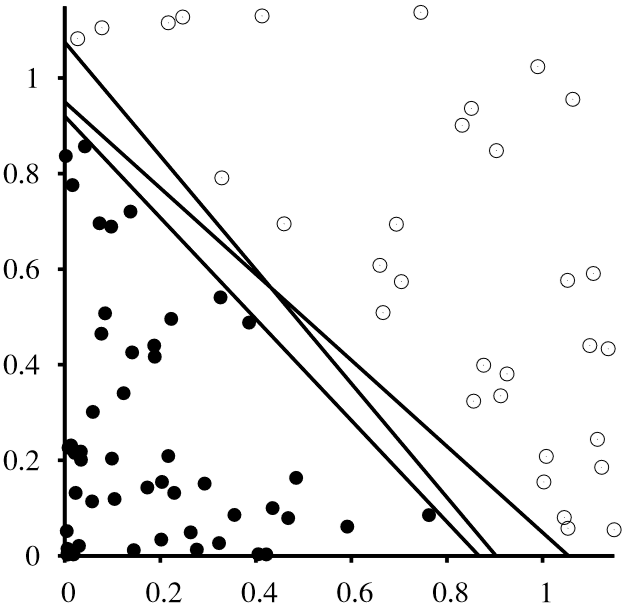
\includegraphics[width=\textwidth]{images/svm0}
        \caption{}
        \label{fig:svm_a}
    \end{subfigure}
    \begin{subfigure}{0.5\textwidth}
        \centering
        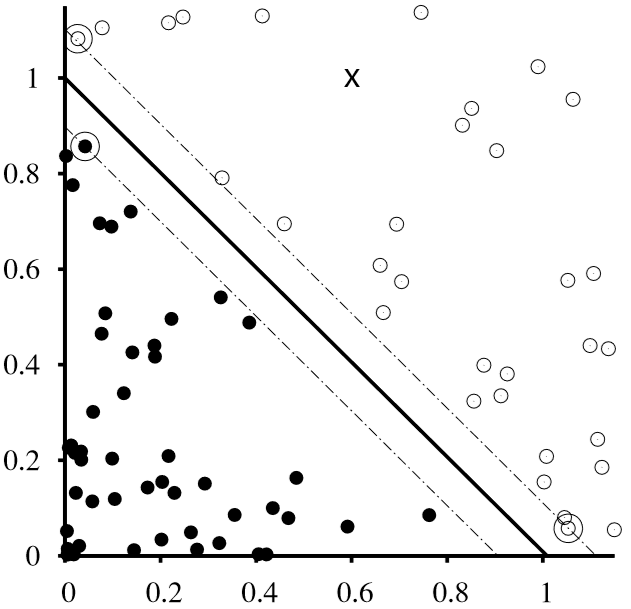
\includegraphics[width=\textwidth]{images/svm1}
        \caption{}
        \label{fig:svm_b}
    \end{subfigure}
\caption{
    Ejemplo sencillo de entrenamiento y clasificación con máquina de vectores soporte con dos clases, blanco y negro.
    (a) Instancias de entrenamiento etiquetadas (puntos blancos y negros) con tres separadores lineales candidatos de ejemplo.
    (b) Separador óptimo con máximo margen (linea sólida) encontrado luego del entrenamiento, el cual está justo en el punto medio del margen entre las dos clases (área entre las lineas puntadas).
    Los \emph{vectores soporte} de dicho separador son señalados con círculos grandes.
    Luego en (a), durante la clasificación, la nueva instancia $\langle 0.6, 1\rangle$ es ingresada (cruz negra), clasificándose como ``blanca'' por ubicarse por encima del separador, en la zona asociada a dicha clase.
}
\label{fig:svm}
\end{figure}

Desarrollado en AT\&T Bell Laboratories por Vapnik \emph{et al.}\cite{boser1992training,guyon1993automatic,cortes1995support,drucker1997support}, la Máquina de Vectores Soporte, o más popularmente conocida por su nombre en inglés como \ac{SVM}, es uno de los mejores, e incluso muchos creen que es el mejor, algoritmo de aprendizaje supervisado ``que viene listo para ser usado'': si uno no tiene ningún conocimiento previo especializado sobre un dominio, \ac{SVM} suele ser un excelente método para probar primero\cite{hsu2003practical}.

De forma abstracta, \ac{SVM} ve a cada instancia $\pmb{x}=\langle x_1,x_2,\dots,x_m\rangle$ como un punto en un espacio $m$-dimensional. Luego, durante el entrenamiento, utiliza todas las instancias de entrenamiento para encontrar el hiperplano óptimo que mejor divida las clases en ese espacio $m$-dimensional, es decir, el que tenga el máximo margen entre las dos clases.\footnote{\ac{SVM}, al ser un clasificador lineal, en principio sólo puede trabajar con dos clases. Sin embargo, esto no es una limitante ya que para trabajar con un número $k$ de clases mayor a 2, simplemente se utilizan $k$ modelos \ac{SVM} distintos, uno por cada clase.}
Así, al finalizar el entrenamiento, se tiene un hiperplano óptimo que divide el espacio $m$-dimensional en dos zonas, una asociada a cada clase. Finalmente, la clasificación se lleva a cabo simplemente viendo en cuales de esas dos zonas se ubica la instancia de entrada, $\pmb{x}$, al proyectarse en ese espacio $m$-dimensional.
Una característica particular de \ac{SVM} es que la solución al problema de clasificación está representada simplemente por los denominados como ``vectores soporte'', que no son otra cosa que las instancias de entrenamiento\footnote{Recordemos que cada instancia está representada como un vector de $m$ atributos, $\pmb{x}=\langle x_1,x_2,\dots,x_m\rangle$, de allí el nombre \emph{vectores} soporte.} más cercanas al separador óptimo.
Por ejemplo, suponiendo que nuestras instancias tuvieran sólo dos atributos, esto es $\pmb{x}=\langle x_1,x_2\rangle$, y pertenecieran a alguna de dos clases, digamos ``blanco'' o ``negro'', la \autoref{fig:svm} ilustra un posible ejemplo de entrenamiento, con el ``hiperplano óptimo'' (o en este caso ``línea óptima'') y sus respectivos vectores soporte, y un ejemplo de clasificación para una nueva instancia de entrada, $\langle 0.6, 1\rangle$.

\ac{SVM} también se pueden utilizar para problemas de clasificación no linealmente separables. En tales casos se utiliza lo que se conoce generalmente como el ``truco del kernel''\cite{scholkopf2001kernel}, en donde, haciendo uso de una función denominada como ``kernel'', las instancias son proyectadas a un nuevo espacio, de mayor dimensión, en donde las clases sí son  linealmente separables.


\subsection{Clasificadores Bayesianos Naïve}
\label{sec:mnb}

Los clasificadores bayesianos son una familia de clasificadores estadísticos que se basan en el teorema de Bayes, los cuales pueden predecir la probabilidad de pertenencia de una instancia dada a cada una de las clases\cite{murphy2006naive, rish2001empirical}. Más precisamente, dada una instancia de entrada a ser clasificada, la cual nuevamente está representada por un vector de $m$ atributos, $\pmb{x}=\langle x_1,x_2,\dots,x_m\rangle$, un clasificador bayesiano es un modelo capaz de calcular la probabilidad condicional, $P(c|\pmb{x})$, para cada una de las posibles clases $c$, clasificando finalmente a $\pmb{x}$ con la clase $c$ más probable de todas. Dado que, a diferencia de $P(c|\pmb{x})$, $P(\pmb{x}|c)$ puede aproximarse de forma directa utilizando todas las instancias $\pmb{x}$ disponibles en el conjunto de entrenamiento, la probabilidad condicional $P(c|\pmb{x})$ se calcula en base a $P(\pmb{x}|c)$ utilizando el teorema de Bayes del siguiente modo:

$$P(c|\pmb{x})=\frac{P(c)P(\pmb{x}|c)}{P(\pmb{x})}$$

Sin embargo, como para clasificar sólo es necesario encontrar la clase más probable, siendo $P(\pmb{x})$ independiente de cualquier clase $c$ y, por lo tanto, constante, para clasificar se prescinde del denominador, llevando a:

\begin{equation}
P(c|\pmb{x})\propto P(c)P(\pmb{x}|c)
\label{eq:mnb0}
\end{equation}


Los tipos de clasificadores bayesianos más ampliamente utilizados son los llamados como ``clasificadores bayesianos naïve'', los cuales suponen \emph{ingenuamente}\footnote{De allí que se utilice el término ``naïve''.} que, dada una categoría $c$, cada atributo $x_i$ de $\pmb{x}$ es condicionalmente independiente de todos los demás atributos $x_j$, con $i\ne j$.
Esta suposición se llama independencia condicional de clase\cite{lewis1998naive} y se utiliza con el fin de simplificar el cálculo de la clasificación, ya que al aplicarla se cumple que:

\begin{equation}
P(\pmb{x}|c)=P(x_1,x_2,\dots,x_m|c) = P(x_1|c)P(x_2|c)\dots P(x_m|c)
\label{eq:mnb1}
\end{equation}

Lo que permite, reemplazando \autoref{eq:mnb1} en \autoref{eq:mnb0}, realizar el cálculo involucrado simplemente en términos del producto de las probabilidades condicionales individuales de cada atributo, tal que así:

$$P(c|\pmb{x}) \propto P(c)P(x_1|c)P(x_2|c)\dots P(x_m|c) = P(c)\displaystyle\prod_{i=1}^{m}P(x_i|c)$$

Por lo que, finalmente, un clasificador bayesiano naïve clasificará a una instancia de entrada $\pmb{x}=\langle x_1,x_2,\dots,x_m\rangle$ calculando dicho producto para todas las clases y  seleccionado la que produzca el mayor resultado. En símbolos, siendo $C$ el conjunto de todas las clases, el clasificador seleccionará la clase $\hat{c}$ tal que:

\begin{equation}
\hat{c}=\argmax_{c\in C} P(c)\displaystyle\prod_{i=1}^{m}P(x_i|c)
\label{eq:mnb-prod}
\end{equation}

Sin embargo, una dificultad fundamental al realizar matemáticas continuas en una computadora digital es la necesidad de representar infinitos números reales con un número finito de bits. Esto significa que para casi todos los números reales se incurrirá en algún error de aproximación cuando sean representados en la computadora.\footnote{Típicamente utilizando números de puntos flotantes.} Una forma de error de redondeo, que es particularmente devastadora, es el \emph{underflow}, el cual ocurre cuando los números cercanos a cero se redondean a cero.
Por ese motivo, el cómputo de la \autoref{eq:mnb-prod} en la práctica falla convergiendo rápidamente a cero, ya que se trata de productos sucesivos de probabilidades (números reales pequeños positivos menores a uno). 
% Desde un punto de vista computacional, debido a la limitada precisión que las computadoras poseen para representar a los números reales utilizando sólo un número finito de bits,\footnote{Típicamente utilizando números de puntos flotantes.} el cómputo de productos sucesivos de números reales positivos menores a $1$ converge rápidamente a $0$.
Afortunadamente, cuando sólo interesa encontrar un valor máximo, como en esta ecuación, este problema normalmente se evita aplicando el logaritmo sobre la secuencia de productos, que de este modo se transforma en una secuencia de sumas.\footnote{Notar que al ser el logaritmo una función monótona creciente, este cambio no altera el resultado final de la ecuación, $\hat{c}$.}
Como consecuencia, los clasificadores bayesianos naïve en la práctica clasifican las instancias de entrada utilizando, en lugar de la \autoref{eq:mnb-prod}, la siguiente ecuación:

% $\log{\Big(P(c)\displaystyle\prod_{i=1}^{m}P(x_i|c)\Big)}$

\begin{equation}
\hat{c}=\argmax_{c\in C} \log{P(c)}+\sum_{i=1}^{m}\log{P(x_i|c)}
\label{eq:mnb-log}
\end{equation}

Finalmente, dependiendo de la tarea a abordar y la distribución de probabilidad que se asuma, será el clasificador en concreto con el que se trabaje y la manera concreta de calcular/aproximar las probabilidades.
Así, si se asume una distribución multinomial, el clasificador en concreto es denominado como ``clasificador bayesiano naïve multinomial'', o más popularmente conocido por su nombre en inglés como clasificador \ac{MNB}.
Por ejemplo, cuando se utiliza \ac{MNB} para abordar tareas de clasificación de texto, cada atributo $x_i$ suele corresponderse con una palabra $w_i$ del vocabulario aprendido, en cuyo caso las probabilidades de la \autoref{eq:mnb-log}, en la práctica, suelen calcularse utilizando la frecuencia de las palabras (estimación por máxima verosimilitud) del siguiente modo:

$$\hat{P}(w_i|c) = \frac{fr_{w_i,c}}{\sum_{w\in V}fr_{w,c}}$$

$$\hat{P}(c) = \frac{N_c}{N}$$

Donde $fr_{w_i,c}$ denota la frecuencia de la palabra $w_i$ en la clase $c$,\footnote{O la frecuencia más uno, en el caso de que se utilice un suavizado Laplace para evitar probabilidades igual a 0 para palabras desconocidas.} $V$ el vocabulario formado por todas las palabras presentes en el conjunto de entrenamiento, $N$ el número total de documentos en el conjunto de entrenamiento, y $N_c$ el número de documentos pertenecientes a la clase $c$. 
El clasificador \ac{MNB} es prácticamente el clasificador bayesiano por antonomasia en tareas de clasificación de texto, ya que al hacer corresponder cada atributo $x_i$ con cada palabra $w_i$, cada cual ocurriendo con una probabilidad $P(w_i|c)$, cada instancia $\pmb{x}=\langle x_1,x_2,\dots,x_m\rangle$ puede verse como una muestra generadas por, o tomada desde, una multinomial $(P(w_1|c),P(w_2|c),\dots,P(w_m|c))$.



\subsection{Redes Neuronales}

\begin{figure}[t]
    \centering
    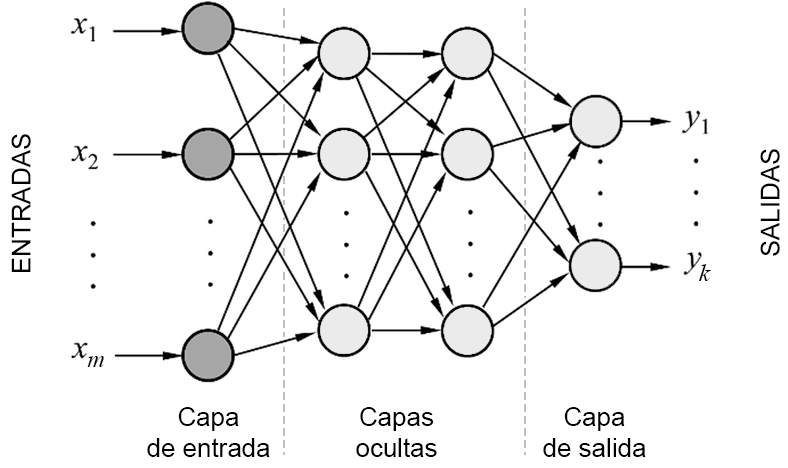
\includegraphics[width=120mm]{images/nn}
    \caption{Ejemplo de red neuronal de $m$ entradas y $k$ salidas. La red está compuesta por una capa de entrada con $m$ nodos de entradas, dos capas ocultas, y una capa de salida con $k$ nodos de salidas.}
    \label{fig:nn}
\end{figure}

Las redes neuronales artificiales, en inglés, \ac{ANN}, son modelos computacionales inspirados en el cerebro humano. Se denominan neuronales porque sus orígenes se encuentran en la ``neurona McCulloch-Pitts'' \cite{mcculloch1943logical}, un modelo simplificado de la neurona humana como una especie de elemento de cómputo que podría describirse en términos de lógica proposicional. Una \ac{ANN} es, en esencia, una red de pequeñas unidades de cómputo denominados como ``nodos'', ``neuronas'' o simplemente ``unidades'', las cuales típicamente se agrupan en distintos niveles, denominados como ``capas''\cite{basheer2000artificial,goodfellow2016deep}. Como se ilustra en la \autoref{fig:nn}, las redes neuronales tiene tres tipos de capas, a saber, de entrada, ocultas y de salida: la capa de entrada está compuesta por todos los nodos que reciben la entrada propiamente dicha, y cuya función es simplemente la de propagar la entrada hacia los nodos internos, sin modificarla; la capa de salida está compuesta por todos los nodos que generan la salida de la red, propiamente dicha; y finalmente, todas las otras capas, entre la entrada y la salida, son denominadas como capas ocultas.

\begin{figure}[t]
    \centering
    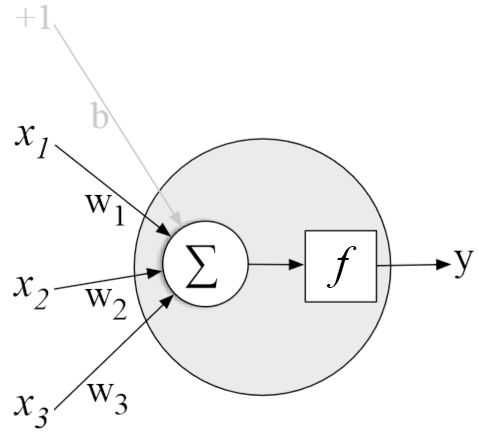
\includegraphics[width=60mm]{images/nn-node}
    \caption{Ejemplo de nodo con 3 entradas, $x_1$, $x_2$ y $x_3$.}
    \label{images/nn-node}
\end{figure}

Como se ilustra en la \autoref{images/nn-node}, cada nodo de una red neuronal toma un vector de valores de entrada, $\langle x_0,x_1,\dots,x_m\rangle$, y produce un único valor de salida, $y$, aplicando una función $f$ al producto punto entre el vector de entrada y un vector de pesos, $\langle w_0,w_1,\dots,w_m\rangle$, que cada nodo tiene asociado. Más precisamente, y en símbolos, la salida $y$ de un nodo se obtiene por:

$$y =  f\left(b + \sum_{i=0}^m w_i x_i\right)$$

La función $f$ se denomina como ``función de activación'' y su rol es determinar si el resultado del producto punto es suficiente como para que dicho nodo ``se active'' o no, esto es, si se propaga un valor de salida positivo ($y>0$) hacia los siguientes nodos o, de lo contrario, no se propaga ningún valor ($y=0$).\footnote{Algunas funciones de activación, como ser $\tanh$, pueden producir valores negativos ($y\leq0$).}
Tres de las funciones de activaciones más utilizadas son la función $softmax$, $tanh$, y $ReLu$\cite{ramachandran2017searching}.

El entrenamiento consiste en encontrar los valores adecuados para los pesos asociados a todos los nodos de la red. Existen distintos métodos para encontrar dichos valores, siendo ``backpropagation''\cite{chauvin1995backpropagation} el algoritmo más ampliamente utilizado actualmente. 
Cuando una \ac{ANN} es utilizada como un clasificador, habrá una nodo de entrada por cada atributo $x_i$ de la instancia de entrada, $\pmb{x}=\langle x_1,x_2,\dots,x_m\rangle$, y un nodo de salida por cada clase de interés. La clasificación se lleva a cabo alimentando a la red con la instancia de entrada, $\pmb{x}$, y asignando la etiqueta asociada al nodo de salida que produce el mayor valor.

\

En la actualidad, con el aumento del poder de cómputo basado en el uso de GPU y la masiva disponibilidad de datos, las redes neuronales normalmente llegan a ser considerablemente profundas, con un gran número de capas ocultas y miles de nodos, lo que permite que se desempeñen asombrosamente bien en una gran variedad de tareas, como ser en el reconocimiento de voz y en el reconocimiento de imágenes. Esto produjo una gran proliferación de distintas arquitecturas de redes profundas, denominadas como ``arquitecturas de aprendizaje profundo''\cite{goodfellow2016deep}. %, tales como redes neuronales recurrentes, redes neuronales convoluciones o redes de creencias profundas.

\subsection{K Vecinos Más Próximos}

El \ac{ABI} es una familia de algoritmos de aprendizaje que, en lugar de realizar una generalización explícita, compara las nuevas instancias de entrada directamente con las instancias disponibles en el conjunto de entrenamiento.
Esto es, en lugar de llevar a cabo una fase de entrenamiento para construir una abstracción con las instancias de entrenamiento, en \ac{ABI} se representa cada instancia de entrada $\pmb{x}$ como un punto en un espacio $m$-dimensional ---en otras palabras, cada instancia es representada por un vector de $m$ atributos, $\pmb{x}=\langle x_1,x_2,\dots,x_m\rangle$. Luego, las nuevas instancias de entradas serán clasificadas directamente en base a las etiquetas que tienen asignadas las instancias de entrenamiento más cercanas, en ese espacio $m$-dimensional.

La idea principal detrás de estos algoritmos es que instancias similares deben pertenecer a categorías similares, es decir, la etiqueta para la entrada debería ser la misma que tienen las instancias cercanas. El concepto de ``cercanía'' implícitamente conlleva la necesidad de definir formalmente el concepto de ``similitud'' entre pares de instancias. Para ello, es necesario utilizar una \emph{función de similitud} que calcula la distancia entre instancias. Además, los modelos basados en \ac{ABI} también tienen que definir una función, o política de clasificación, que especifique cómo se clasificará efectivamente la entrada en base a las etiquetas de las instancias cercanas.

Existen varios clasificadores basados en \ac{ABI} tales como el ``k Vecinos Más Próximos'' y el algoritmo K*, entre otros\cite{witten2002data}. De entre estos, el más ampliamente utilizado es el primero, ``k Vecinos Más Próximos'', que es más conocido por su nombre en inglés como \ac{k-NN}.

\ac{k-NN} se basa en el algoritmo ``Vecino Más Próximo''\cite{cover1967nearest}, el cual usando alguna función de distancia dada\cite{prasatha2017effects},\footnote{Típicamente distancia coseno, euclidiana, o Manhattan.} determina cuál de todas las instancias del conjunto de entrenamiento es la más similar a la instancia dada, clasificando a esta última con la misma etiqueta que tiene asignada esta instancia más cercana.
\ac{k-NN} generaliza este algoritmo, encontrando no sólo la instancia más cercana, sino las $k$ instancias más cercanas a la nueva, clasificándola, finalmente, en base a la etiqueta que predomina entre todas ellas\cite{zhang2017efficient}.


\subsection{Árboles de Decisión}


\begin{figure}
    \centering
    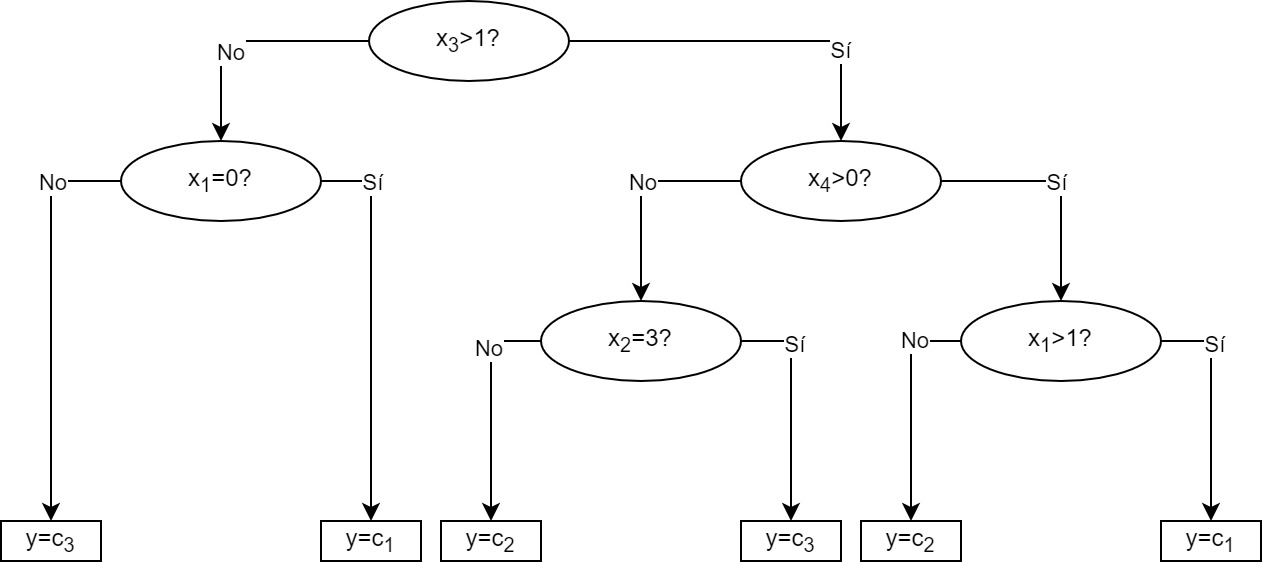
\includegraphics[width=\textwidth]{images/dt}
    \caption{Ejemplo sencillo de un árbol de decisión.}
    \label{fig:ad}
\end{figure}


Los \ac{AD} fueron aplicados por primera vez al modelado del lenguaje por Bahl \emph{et al.} para estimar la probabilidad de las palabras habladas\cite{bahl1989tree}.
Un árbol de decisión es una representación gráfica en la que cada nodo interno está asociado a una decisión sobre uno de los atributos que conforman la entrada, y los nodos terminales (hojas) están asociados con una etiqueta de clase.
Más en concreto, cada nodo interno está normalmente asociado a una condición lógica, la cual puede ser verdadera o falsa, sobre un atributo en particular de la entrada\cite{breslow1997simplifying}.%, que a su vez se enlaza con nuevos nodos en relación a cada posible respuesta a dicha decisión.
Por ejemplo, suponiendo que la entrada está conformada por 4 atributos, en símbolos, $\pmb{x}=\langle x_1,x_2,x_3,x_4\rangle$, y la salida $y$ puede tomar valores de etiqueta, $y\in\{c_1,c_2,c_3\}$, entonces un ejemplo de árbol de decisión podría ser el mostrado en \autoref{fig:ad}.

La construcción de los \ac{AD} generalmente implica un proceso recursivo de división del conjunto de entrenamiento para elegir el atributo de cada nodo interno. Así, se comienza seleccionando el atributo más relevante/discriminativo para todo el conjunto de entrenamiento como raíz del árbol.
Luego se crea un nuevo subárbol hijo por cada posible respuesta a la condición lógica de este nodo raíz. Finalmente, cada subárbol se construye recursivamente siguiendo este mismo proceso, usando sólo un subconjunto del conjunto de entrenamiento, obtenido al dividirlo según la condición lógica asociada a dicho subárbol.
Uno de los principales problemas a la hora de construir un árbol de decisiones es determinar qué atributo debe elegirse como ``el más relevante''. Un atributo relevante debe poder dividir, tanto como sea posible, las instancias de entrenamiento entre las diferentes clases.
Para llevar a cabo esto, en la práctica se utilizan medidas provenientes de la Teoría de la Información\cite{shannon1948mathematical}, como la entropía, la entropía relativa, la complejidad de Kolmogorov, entre otras\cite{chandola2009anomaly}.

Los \ac{AD} representan el ``estándar de oro'' de los modelos basados en el paradigma ``divide y vencerás''. Sin embargo, el tamaño, la complejidad y la dispersión de datos suelen conducir a clasificaciones erróneas cuando los árboles se vuelven lo suficientemente grandes.



\section{Evaluación de Clasificadores}

Una vez seleccionado el modelo de clasificación a utilizar, y de entrenarlo con los datos disponibles en el conjunto de entrenamiento, es necesario poder saber si realmente el modelo funciona, es decir ¿es posible confiar en sus predicciones? ¿Podría el modelo simplemente haber memorizado los datos con los que se lo entrenó y, por lo tanto, en la práctica no desempeñarse adecuadamente con nuevas instancias?
La capacidad de un modelo de clasificar correctamente nuevas instancias desconocidas se denomina como \emph{capacidad de generalización}\cite{schmidhuber1997discovering,xu2017information}.
Así, en el aprendizaje automático, es crucial poder evaluar cada modelo para poder cuantificar qué tan buena es su capacidad de generalización en el problema en particular que está siendo abordado.
Evaluar el modelo con los datos utilizados para el entrenamiento no es aceptable, ya que puede generar fácilmente modelos sobreoptimistas y sobreajustados, por lo que la evaluación siempre debe utilizar un conjunto de instancias nunca antes vistas.
Existen dos métodos para llevar esto a cabo como parte del proceso de desarrollo del modelo, ``retención'' y ``validación cruzada''.
El primer método consiste en dividir aleatoriamente el conjunto de datos etiquetados completo en tres subconjuntos, denominados como ``entrenamiento'', ``validación'' y ``prueba'', utilizando sólo el primero para entrenar y reteniendo los últimos dos para utilizarlos del siguiente modo:

\begin{itemize}
    \item \textbf{Conjunto de validación}: se utiliza para ajustar y evaluar el rendimiento del modelo durante la fase de entrenamiento. Es decir, proporciona una plataforma de prueba para ajustar los hiperparámetros del modelo, permitiendo seleccionar los mejores posibles.\footnote{Por lo tanto, los modelos sin parámetros pueden prescindir de este conjunto de validación.}
    \item \textbf{Conjunto de prueba}: como está formado por instancias nunca vistas y que, a diferencia del anterior, no interfieren en el entrenamiento, este conjunto se utiliza para evaluar efectivamente el (probable) rendimiento futuro del modelo. Por ejemplo, si el modelo se desempeña mucho mejor con el conjunto de validación que con este conjunto, el modelo no generaliza bien y probablemente la causa sea que la combinación de hiperparámetros seleccionada estén sobreajustados a los datos de entrenamiento.
\end{itemize}

Finalmente, el método ``validación cruzada'' también implica dividir el conjunto de datos etiquetados completo en subconjuntos, pero esta división forma parte de un proceso iterativo. El modelo se entrena y se evalúa con distintos subconjuntos complementarios en cada iteración y, una vez finalizado el proceso, los resultados obtenidos en cada iteración se promedian para dar una estimación del rendimiento general del modelo\cite{seni2010ensemble}.

La técnica de validación cruzada más común es la llamada ``validación cruzada de $k$ iteraciones'', en donde el conjunto de datos original se divide en $k$ subconjuntos de igual tamaño, denominados como ``pliegos''. El valor de $k$ es especificado por el usuario, siendo 3, 4, 5 o 10 los más usados, típicamente dependiendo del tamaño total del conjunto de datos.
Luego, en cada una de las $k$ iteraciones, se selecciona un nuevo pliego para ser utilizado como conjunto de prueba,\footnote{O validación, dependiendo de si se haya reservado un conjunto aparte para ser usado como conjunto de prueba luego de la validación cruzada o no.} y el conjunto de entrenamiento se forma juntando los $k-1$ pliegos restantes.
La ``validación cruzada de $k$ iteraciones'' es una técnica extremadamente popular debido a su robustez, ya que cada instancia de dato llega a estar en un conjunto de prueba exactamente una vez, y llega a estar en un conjunto de entrenamiento $k-1$ veces. Esto reduce significativamente el riesgo de sesgo y sobreajuste, debido a que se utilizan la mayoría de los datos tanto para entrenar como para probar el modelo. 

\

Hasta aquí hemos hablado sobre los métodos para evaluar los modelos dentro del proceso de desarrollo de los mismos, pero no se ha hablado sobre cómo se mide efectivamente su desempeño.
En la siguiente subsección se describen brevemente las medidas de evaluación más ampliamente utilizadas para llevar a cabo dicha tarea.


\subsection{Medidas de Desempeño}
\label{sec:medidas}

Una medida de desempeño cuantifica el rendimiento de un modelo predictivo e implica comparar la etiqueta de clase esperada con la etiqueta de clase predicha.
Existen una gran variedad de métricas estándares que se utilizan ampliamente para evaluar modelos de clasificación\cite{ferri2009experimental}, diseñadas para obtener la fracción, la proporción o la tasa con la que la clase predicha no coincide con la esperada en un conjunto de datos de prueba/evaluación.

Quizás una de las métricas más utilizada es el ``accuracy'', la cual nos indica la proporción de instancias que fueron correctamente clasificadas, esto es:

\begin{equation}
accuracy = \frac{clasificaciones\ correctas}{clasificaciones\ totales}
\label{eq:accuracy}
\end{equation}

El \emph{accuracy} parece lo bastante adecuado, sencillo e intuitivo como para ser usado en cualquier problema a abordar. Sin embargo, esta medida no hace distinciones entre clases, es decir, las respuestas correctas se tratan por igual independientemente de la clase. A veces esto no es adecuado ya que es posible que se desee conocer cuántas instancias fallaron en cada clase. Éste sería el caso si el costo de una clasificación errónea varía según la clase o si se tienen muchos más datos de prueba para una clase que para otra. Por ejemplo, clasificar a un usuario de Twitter como ``depresivo'' cuando no lo es (falso positivo) tiene consecuencias muy distintas a clasificarlo como ``no depresivo'' cuando en realidad sí lo es (falso negativo).

Es por este motivo que muchas veces una manera mucho más adecuada de evaluar el desempeño de un clasificador es utilizando la denominada ``matriz de confusión'', cuya idea general es contar el número de veces que las instancias de cierta clase se clasifican como otra o no.\footnote{Es por esto que se denomina ``matriz de confusión'', ya que hace que sea fácil ver si el clasificador \emph{confunde} las clases, etiquetando incorrectamente con frecuencia a una como otra.}

Más precisamente, una matriz de confusión es una tabla en la que cada fila se corresponde con una clase y contiene el número de instancias predichas para esa clase, desagregadas, a su vez, en columnas, según la clase real de dichas instancias\cite{powers2011evaluation}.
Esto permite visualizar rápidamente el número total de falsos positivos, falsos negativos, verdaderos positivos y verdaderos negativos. Por ejemplo, la siguiente tabla muestra dónde se ubicarían estos valores en una matriz de confusión de $2\times2$ para dos clases hipotéticas, ``Positivo'' y ``Negativo'':

\

\begin{tabular}{l l|c|c|c}
\multicolumn{2}{c}{}&\multicolumn{2}{c}{Realidad}&\\
% \cline{3-4}
\multicolumn{2}{c|}{} & Positivo & Negativo\\
\cline{2-4}
\multirow{2}{*}{Predicción}& Positivo & \begin{tabular}{@{}c@{}}Número de \\ Verdaderos Positivos \\ (\#VP)\end{tabular} &  \begin{tabular}{@{}c@{}}Número de \\ Falsos Positivos \\ (\#FP)\end{tabular} \\
\cline{2-4}
& Negativo & \begin{tabular}{@{}c@{}}Número de \\ Falsos Negativos \\ (\#FN)\end{tabular} & \begin{tabular}{@{}c@{}}Número de \\ Verdaderos Negativos \\ (\#VN)\end{tabular}\\
\cline{2-4}
\end{tabular}

\

La matriz de confusión habilita un análisis más detallado que la mera proporción de clasificaciones correctas dada por el \emph{accuracy}, ya que,  además, brinda información sobre qué clases se predicen correctamente, cuáles incorrectamente y qué tipo de errores se están cometiendo.
Sin embargo, en lugar de utilizar la matriz de confusión completa, a menudo es conveniente utilizar medidas de desempeño que capturen, y resuman en un único valor, cierta información específica presente en la matriz que sea de especial interés para el problema abordado.
Dentro de estas medidas, las más ampliamente conocidas y utilizadas son ``precision'', ``recall'', y ``$F_\beta$''. La primera responde a la pregunta ``de las instancias que el clasificador predijo como de cierta clase, ¿cuántas realmente lo fueron?''; la segunda responde a ``de todas las instancias que pertenecen a cierta clase, ¿cuántos fueron efectivamente clasificadas como tal?''; mientras que la tercera simplemente combina estas dos primeras en una sola, intentando equilibrar ambos aspectos.

Más precisamente, la \emph{precision}, a veces denotada por $\pi$\cite{sebastiani2002machine}, puede interpretarse como la probabilidad de que una predicción positiva\footnote{Por ``positiva'', ``positivo'' o ``clase positiva'' entenderemos aquí, y hasta el final del capítulo, como la clase de nuestro interés, es decir, aquella que estemos interesados en medir.} realmente lo sea. Esta métrica nos sintetiza el porcentaje de instancias clasificadas como positivas que efectivamente lo fueron, en fórmula:

\begin{equation}
precision = \frac{\#VP}{\#VP + \#FP}
\label{eq:precision}
\end{equation}


De igual modo, el \emph{recall}, a veces denotada por $\rho$\cite{sebastiani2002machine}, sintetiza el porcentaje de todas las instancias positivas que fueron, efectivamente, clasificadas correctamente, calculándose como:

\begin{equation}
recall = \frac{\#VP}{\#VP + \#FN}
\label{eq:recall}
\end{equation}

Finalmente, como se mencionó anteriormente, la medida $F_\beta$ busca combinar \emph{precision} y \emph{recall} a través de una media armónica que mide la efectividad de la clasificación teniendo en cuenta que se le da, proporcional a $\beta$, una importancia  mayor al \emph{recall} que a la \emph{precision}. Más precisamente, y en símbolos, se tiene que:

\begin{equation}
F_\beta = (1 + \beta^2) \times \frac{precision\times recall}{\beta^2 \times precision + recall}
\label{eq:fbeta}
\end{equation}


Dado que $\beta=1$ indicaría que se da igual importancia tanto a \emph{recall} como a \emph{precision}, $F_1$ es con frecuencia la medida $F$ más ampliamente utilizada:

\begin{equation}
F_1 = 2 \times \frac{precision\times recall}{precision + recall}
\label{eq:f1}
\end{equation}

Notar que el valor $F_1$ será pequeño si alguno de los dos, \emph{precision} o \emph{recall}, lo son, ya que, a diferencia de la media aritmética, la media armónica tiende hacia el menor de los valores ---por lo tanto, su valor se maximiza sólo cuando los valores están ``en armonía'', \emph{i.e.} cuando ambos valores son cercanos entre sí.
\hfill$\square$


%\acresetall
%\chapter{Clasificación de Texto}
%\label{cap3}
%A la fecha, la \emph{World Wide Web (WWW)} contiene más de 5.470 millones de páginas Web indexadas\cite{www2020}, en su gran mayoría, conteniendo información escrita en lenguaje natural. Si tuviéramos que imprimir todo este contenido en papel, y siendo muy conservadores,\footnote{Suponiendo, ingenuamente, que cada página web requiere, en promedio, de 30 hojas para imprimirse\cite{harwood2015much}.} requeriríamos al menos de 164.100 millones de páginas A4 para lograrlo.
En este contexto, es beneficioso contar con sistemas computacionales que sean capaces de procesar, adquirir, extraer información útil y realizar tareas valiosas, a partir del texto en crudo.
El diseño y desarrollo de dichos sistemas es uno de los problemas más desafiantes dentro de la \ac{IA}, ya que estos sistemas necesitan entender, en cierta medida, el lenguaje ambiguo, desordenado, y poco estructurado usado por nosotros, los humanos.
Tal es la relevancia de este desafiante problema que su origen puede rastrearse incluso hasta los orígenes de la \ac{IA} como tal, ya que, cuando Alan Turing propone su famoso ``test de Turing''\cite{turing2009computing}\footnote{Originalmente llamado ``The Imitation Game''.} como definición pragmática de inteligencia, lo hace en relación a la capacidad de los sistemas para procesar y comprender el lenguaje natural de su interlocutor.
En este capítulo, nos restringiremos a examinar una tarea específica dentro de esta problemática, denominada como \emph{clasificación de texto}, que, si bien tal vez pueda parecer acotada, en la práctica tiene una amplia aplicabilidad.



\section{Introducción}

En la \autoref{sec:clasificacion} del capítulo anterior se introdujo el concepto de \emph{clasificación} dentro del marco del aprendizaje automático supervisado. Aquí nos centraremos en una tarea de clasificación específica, conocida como clasificación de texto:\footnote{También conocida como \emph{categorización de texto}.} \emph{dado un texto de entrada, decidir a cuál de un conjunto predefinido de clases pertenece}.
Algunos ejemplos de aplicaciones reales de clasificación de texto serían el análisis de sentimientos en reseñas de películas o productos (clasificar una reseña como positiva o negativa), filtrado de spam (clasificar un e-mail como ``spam'' o ``no spam''), identificación automática de idiomas, categorización temática (clasificar documentos de acuerdo a su temática), así como también, la tarea abordada en este trabajo doctoral, esto es, la detección anticipada de riesgos, tales como depresión, anorexia o conductas autodestructivas, en base al contenido generado por el usuario en redes sociales.

En el capítulo anterior también vimos que los modelos de clasificación trabajan con instancias de entrada representadas por vectores de $m$ atributos, $\pmb{x}=\langle x_1,x_2,\dots,x_m\rangle$.
Esto implica que, en principio, el texto no puede ser interpretado directamente por los modelos, no sin antes ser procesado y transformado adecuadamente. Para llevar esto a cabo, normalmente se sigue un proceso que puede ser dividido en, al menos, dos etapas principales: una etapa encargada de preprocesar el texto y otra relacionada a la transformación del mismo a una representación vectorial propiamente dicha. Así, este capítulo se organiza de la siguiente manera: en la siguiente sección, \autoref{sec:preprocesado}, se describe brevemente esta primer etapa de preprocesamiento, mientras que la segunda es abordada en la \autoref{sec:representacion}, en donde se examinan distintos enfoques para representar el texto como un vector de atributos. Finalmente, la \autoref{sec:EC} introduce formalmente la problemática abordada en este trabajo de investigación, enmarcándolo como un escenario particular de clasificación de texto.
Por este motivo, los lectores ya familiarizados con la clasificación de textos, pero no con la problemática abordada, pueden continuar su lectura directamente a partir de la última sección.

\section{Preprocesamiento}
\label{sec:preprocesado}

% En clasificación de texto, a cada instancia de entrada se la denomina típicamente como documento de entrada.
El preprocesamiento consiste básicamente en la preparación del texto para su posterior procesamiento.
De forma general, preprocesar el texto simplemente significa llevarlo a una forma ``estándar'' que sea predecible y analizable, lo que ``estándar'' realmente signifique dependerá de  la tarea abordada y, muchas veces, también del clasificador utilizado.
La elección del preprocesamiento adecuado puede mejorar significativamente el desempeño de la clasificación\cite{uysal2014impact,hacohen2020influence}.
Sin embargo, el preprocesamiento de texto no es directamente transferible ni de una tarea a otra, ni de un modelo a otro ---puede ocurrir que el preprocesamiento ideal para una tarea, o para un modelo, se convierta en la peor opción para otro.

Existen diferentes tipos de técnicas de preprocesamiento de texto que pueden aplicarse en simultáneo sobre el texto de entrada. Estas técnicas pueden variar desde lo simple, como ser una sencilla conversión del texto a letras minúsculas, hasta lo elaborado, como ser la corrección automática de errores ortográficos o el enriquecimiento del texto usando etiquetadores gramaticales.
Sin embargo, ya que el preprocesamiento consta típicamente de tres etapas bien definidas, las técnicas estarán asociadas a cada una de estas etapas del siguiente modo: 

\begin{itemize}
    \item\textbf{Eliminación de ruido:} como su nombre lo indica, esta etapa se encarga de la eliminación del ruido en el texto de entrada con el fin de obtener el texto crudo. De entre todas, esta etapa es la que más depende del problema específico que está siendo abordado, ya que dependerá del dominio en el que se esté trabajando y el formato del texto de entrada, lo que implique ruido o no.
    Ejemplos de eliminación de ruido podrían ser la eliminación de palabras clave específicas al dominio, como ser ``RT'' para retweet, la eliminación de metadatos, tales como encabezados específicos de ciertos archivos, o la eliminación de información de formato o presentación, como las etiquetas HTML/XML.
    
    \item\textbf{Tokenización:} en es
    ta etapa se divide el texto en partes más pequeñas o ``tokens''. Por ejemplo, trozos grandes de texto pueden tokenizarse en oraciones y las oraciones tokenizarse en palabras.
    %En ocasiones, a la tokenización también se la suele conocer como ``segmentación de texto'' o ``análisis léxico''.
    Muy a menudo se suele reservar el término ``tokenización'' exclusivamente para la división del texto en palabras individuales, y el término ``segmentación'' para la división en bloques más grandes, como ser párrafos u oraciones.
    En esta etapa se pueden utilizar distintas técnicas, tanto para identificar los límites de los distintos segmentos como para determinar qué hacer una vez se los identifica.
    En cualquier caso, una vez que el texto ha sido tokenizado adecuadamente, generalmente, se procede con el resto del preprocesamiento.\footnote{En ciertos idiomas, por ejemplo, idiomas aglutinantes como el alemán o el japonés, esta etapa también tiene que ver con separar palabras compuestas en sus monemas independientes.}
    
    \item\textbf{Normalización:} esta etapa se refiere, generalmente, a la aplicación de una serie de tareas con el fin de dejar a todo el texto en ``igualdad de condiciones''.
    De este modo, la normalización permite que el procesamiento de las entradas proceda de manera uniforme, independientemente de cómo eran dichas entradas originalmente.
    Esta etapa, normalmente, involucra alguna(s) de las siguientes tareas: convertir todo el texto a minúsculas (o mayúsculas), eliminar las signos de puntuación, eliminar o convertir los números a su equivalente en palabras, eliminar las \emph{palabras vacías},\footnote{En el campo del \ac{PLN}, se utiliza el término ``palabra vacía'', en inglés ``stop word'', para referirse a una palabra que carece de semántica en relación al problema abordado. A excepción de problemas muy específicos, las palabras vacías se corresponden con las ``palabras funcionales'' en lingüística, \emph{i.e.} palabras que desempeñan un papel dentro del lenguaje en sí mismo sin referir a la realidad extralingüística. Por este motivo, en la práctica es habitual la utilización del término ``palabra vacía'' para referirse a palabras tales como artículos, preposiciones o conjunciones.} eliminar palabras de muy baja frecuencia, enriquecer/aumentar el texto con información valiosa para el problema abordado y reemplazar palabras por su raíz.
    Siendo \emph{stemming} y \emph{lemmatization} las dos técnicas más utilizadas para llevar a cabo esta última tarea.
    El primero construye la raíz simplemente eliminando los afijos (típicamente los sufijos) de las palabras,\footnote{Por ejemplo, ``pensaba'' se reemplazaría por ``pens'' tras la eliminación del sufijo ``aba''.} mientras que el segundo, más elaborado, usa el lema de la palabra como su raíz.\footnote{Por ejemplo, las tres palabras, ``pensaba'', ``pensábamos'' y ``pensando'' se reemplazarían por el lema, ``pensar''.}
\end{itemize}


En la práctica, dependiendo de la tarea, cualquiera de estas etapas podrá o no aplicarse. De hecho, estas etapas no necesariamente representan un proceso lineal cuyos pasos deben aplicarse exclusivamente en el orden dado.

\section{Representación}
\label{sec:representacion}

Como se mencionó al comienzo, típicamente, el texto no puede ser interpretado directamente por un clasificador, por lo que una vez preprocesado, el siguiente paso a definir es cómo se lo representará para poder ser efectivamente ingresado al modelo de clasificación.
Esto es, se debe definir qué procedimiento se utilizará para mapear el texto de un documento, $d$, a una representación vectorial de su contenido, $d=\langle w_1,\dots,w_m\rangle$.
La elección de una representación adecuada suele ser uno de los aspectos más imperantes, sino el más, de la creación de un buen clasificador.
A su vez, los distintos tipos de representaciones dependen principalmente de lo que se consideren como las unidades significativas del texto y la semántica de cada una de ellas~\cite{turney2010frequency}.
Así, de acuerdo a los objetivos de esta tesis, nos limitaremos a identificar y describir dos tipos de representaciones fundamentales: representaciones dadas por léxico y representaciones dadas por contexto.
En la primera, el texto es modelado como una secuencia de unidades léxicas, mientras que la segunda intenta capturar el significado de las palabras en base al contexto en el que éstas aparecen. El resto de esta sección está destinada a examinar brevemente estos dos grupos de representaciones.


\subsection{Representaciones dadas por Léxico}


Según la Real Academia Española, se define a léxico como el conjunto de palabras que conforman un determinado vocabulario.
En este contexto, las representaciones dadas por léxico hacen referencia a las representaciones que se basan en la construcción de un vocabulario utilizando los documentos del conjunto de entrenamiento.
Este vocabulario no necesariamente estará formado por palabras, sino que, de forma general, estará formado por cualquier tipo de unidades léxicas, tales como trozos de palabras, palabras individuales o, incluso, cadenas de palabras.
En la clasificación de texto, a estas unidades léxicas se las conoce como \textbf{términos}, por lo que es habitual denominar a este vocabulario como ``vocabulario de términos''.

De esta forma, para construir la representación de un documento $d$, primero se procesa el texto como una secuencia de términos\footnote{Este secuencia de términos normalmente se crea dividiéndolo durante la etapa de tokenización del preprocesamiento.} y luego se lo convierte en un vector $d=\langle w_1,\dots,w_m\rangle$, donde $m$ es el número total de términos en el vocabulario, y $w_i$ es el valor, denominado como ``peso'', asociado al $i$-ésimo término del vocabulario.
Este peso representa, hablando vagamente, cuánto contribuye cada término en particular a la semántica del documento $d$.
Por lo que, distintas representaciones particulares surgirán de las diferentes formas de entender qué es un término y de las diferentes formas de calcular el pesado de los mismos. En las siguientes dos subsecciones, tituladas ``Tipos de Términos'' y ``Pesado de Términos'', se examinan respectivamente ambos aspectos.

\subsubsection{Tipos de Términos}
\label{sec:tipo-termino}

A la hora de representar documentos, sin duda, la elección más ampliamente utilizada es identificar a los términos con las palabras individuales. A esta representación se la conoce con el nombre particular de \textbf{bolsa de palabras} o simplemente como \emph{BoW}, del inglés \emph{Bag of Words}. 
Este nombre surge de que, bajo esta suposición, se puede pensar a cada documento como una bolsa en la que se han puesto todas sus palabras, una a una, y, luego, se utilizará esta última para construir la representación, en lugar del documento original.
A pesar de su simpleza, la representación de bolsa de palabras es uno de los  enfoques más efectivos \cite{nguyen2013old,stamatatos2009survey,sebastiani2002machine}, y en la práctica es muy común encontrar que representaciones más sofisticadas no produzcan una mejora significativa de rendimiento \cite{apte1994automated,dumais1998inductive,lewis1992evaluation}.
Sin embargo, a pesar de su amplio uso y efectividad, existen algunos inconvenientes que pueden provocar que su aplicabilidad no sea adecuada en algunos escenarios.
Por ejemplo, al utilizar esta representación, la noción de orden entre las palabras se pierde y, por lo tanto, el modelo clasificará de la misma manera a cualquier permutación posible del texto original y será incapaz de capturar secuencias de palabras importantes ---lo que para algunas tareas sí puede ser relevante. Además, en escenarios donde hay grandes vocabularios, pero pocos documentos de entrenamiento y clases desequilibradas, esta representación puede contribuir a favorecer a las clases mayoritarias por sobre las demás\cite{stamatatos2008author}.

Una de las formas más habituales para intentar mitigar algunas de las limitaciones de la representación de bolsa de palabras es identificar a los términos con secuencias de palabras, en lugar de con palabras individuales. De esta forma, la representación mantiene, en cada término, alguna noción local del orden de las palabras del documento original.
Dado que una secuencia de símbolos de longitud $n$ se llama como \emph{n-grama}, del griego \textgreek{γραμμα} (\emph{gramma}) letra o escrito, a esta representación se la conoce con el nombre de \textbf{representación de \emph{n-grama} de palabras}, siendo casos especiales ``unigrama'' para \emph{1-grama},\footnote{De aquí que a la representación de bolsa de palabras también se la pueda llamar como representación de unigrama de palabras.} ``bigrama'' para \emph{2-grama} y ``trigrama'' para \emph{3-grama}.
Si bien esta representación puede tener cualidades semánticas superiores con respecto a la representación de bolsa de palabras, también sufre de cualidades estadísticas inferiores, ya que, conforme mayor sea el orden del \emph{n-grama}, menor será la frecuencia con la que aparezcan los términos (\emph{i.e.} los \emph{n-gramas de palabras}) en los documentos de entrenamiento\cite{lewis1992evaluation}.\footnote{La probabilidad con la que aparece una secuencia de palabras nunca será mayor que la probabilidad individual de cada palabra.}

Finalmente, en última instancia, un texto escrito no es más que una secuencia de caracteres, por lo que tiene sentido representarlo como tal. Así, otra elección, también muy habitual, es identificar a los términos con secuencias de caracteres, en cuyo caso la representación es denominada como \textbf{representación de \emph{n-gramas} de caracteres}.
Por medio de esta representación, los clasificadores son capaces de capturar no sólo contenido \emph{per se}, sino también información estilística y contextual\cite{stamatatos2009survey}.
Además, también suelen ser más resistentes a los errores ortográficos que las representaciones basadas en palabras completas. Por ejemplo, las palabras ``Paris'' y ``Pariz'' serán consideradas como dos términos completamente distintos por estos últimos, mientras que utilizando una representación de, digamos, trigrama de caracteres, ambas palabras aportarían, en gran medida, el mismo valor a la clasificación final, ya que ambas serán vistas como los términos ``Par''  y ``ari'', más una discrepancia en los términos finales (``ris'' y ``riz'') dada por el error ortográfico.
Sin embargo, a pesar de estas ventajas, también existen algunas desventajas con respecto a las representaciones basadas en palabras completas, como ser la alta dimensionalidad en la representación vectorial final.

\

Antes de finalizar esta subsección, es adecuado resaltar nuevamente que, en las tareas de clasificación de textos, cada problema específico tendrá sus propias particularidades, por lo que podrá ocurrir que la representación ideal para una tarea no sea conveniente para otra.
Por ejemplo, mientras que en tareas de clasificación de tópicos los términos más valiosos suelen ser las palabras temáticas, capturadas fácilmente por representaciones de bolsa de palabras, en tareas de atribución de autoría o detección de plagio, lo suelen ser los n-gramas de caracteres capturando información estilística, ya que el objetivo principal es modelar el estilo de escritura de un autor\cite{stamatatos2009survey}.
 
\subsubsection{Pesado de Términos}

Hasta aquí se han visto los distintos tipos de términos que se pueden utilizar para representar a los documentos, en esta subsección examinaremos brevemente aspectos relacionados a cómo pesarlos, \emph{i.e.} vinculados a cómo calcular los valores $w_i$ asociados a cada término, en el vector que representa al documento, $d=\langle w_1,\dots,w_m\rangle$.

En la práctica, por diversos motivos, tales como herencia por legado del campo de la \emph{Recuperación de Información},\footnote{En las ciencias computacionales, es el campo que históricamente se encarga de la búsqueda y recuperación de documentos que son relevantes en relación a la información necesitada por un usuario dado.} conveniencia matemática y  eficiencia computacional, el cálculo de los pesos, $w_i$, de cada término se calcula en primera instancia construyendo una matriz, denominada como \textbf{matriz documento-término}, que agrupa los vectores de todos los documentos del conjunto de entrenamiento, uno encima del otro.
De esta manera, si se tienen $n$ documentos de entrenamiento y el tamaño del vocabulario es de $m$ términos, la matriz resultante será de $n\times m$, ya que las filas se corresponden a los documentos y las columnas a los términos del vocabulario, como se ilustra en la siguiente figura:

\begin{center}
\begin{tabular}{c|c|c|c|c|c|}
\multicolumn{1}{c}{} & \multicolumn{1}{c}{$t_1$} & \multicolumn{1}{c}{$t_2$} & \multicolumn{1}{c}{$\dots$} & \multicolumn{1}{c}{$t_{m-1}$} & \multicolumn{1}{c}{$t_m$} \\
\cline{2-6}
$d_1$ & & & & & \\
\cline{2-6}
$d_2$ & & & & & \\
\cline{2-6}
$\vdots$ & & & & & \\
\cline{2-6}
$d_{n-1}$ & & & & & \\
\cline{2-6}
$d_n$ & & & & & \\
\cline{2-6}
% \cline{2-6}
% $d_1$ & $w_{1,1}$ & $w_{1,2}$ & $\dots$ & $w_{1,m-1}$ & $w_{1,m}$\\
% \cline{2-6}
% $d_2$ & $w_{2,1}$ & $w_{2,2}$ & $\dots$ &  $w_{2,m-1}$ & $w_{2,m}$\\
% \cline{2-6}
% $\vdots$ & $\vdots$ & $\vdots$ & $\vdots$ & $\vdots$ & $\vdots$ \\
% \cline{2-6}
% $d_{n-1}$ & $w_{n-1,1}$ & $w_{n-1,2}$ & $\dots$ & $w_{n-1,m-1}$ & $w_{n-1,m}$\\
% \cline{2-6}
% $d_n$ & $w_{n,1}$ & $w_{n,2}$ & $\dots$ & $w_{n,m-1}$ & $w_{n,m}$\\
% \cline{2-6}
\end{tabular}
\end{center}

Donde $d_i$ y $t_j$ denotan los índices asociados, respectivamente, al $i$-ésimo documento y al $j$-ésimo término.
Esta matriz permite visualizar claramente la relación entre los términos y los documentos, ya que utilizando sus índices se puede obtener el valor $w_{i,j}$ para cualquier par documento-término.
% Naturalmente, la mayoría de los documentos no contendrán a la mayoría de los términos, por lo que esta matriz no será densa, sino dispersa.\footnote{Es decir, la mayor parte de sus elementos serán cero.}

Luego, distintos tipos de pesados de términos surgen de distintas maneras de completar esta matriz documento-término.
Así, una primera opción es asignarle un 1, o un 0, a cada posición, dependiendo de si el término está presente, o no, en el documento; en cuyo caso a la matriz se la denomina como \emph{matriz documento-término binaria}.
Una segunda opción de granulo más fino sería, en lugar de valorar a cada término simplemente por su ausencia o presencia en el documento, hacerlo por la cantidad de veces que se hizo presente. De esta forma, los términos más frecuentes en un documento serán ``más pesados'' (\emph{i.e.} más valiosos) que los menos frecuentes.
Sin embargo, al utilizar este pesado, el valor de los términos de cada documento estará ligado directamente a su tamaño.\footnote{Pensar, por ejemplo, el siguiente documento pequeño de cuatro palabras: ``la clasificación de texto''. Cada palabra tiene una frecuencia igual a 1, ahora pensar la frecuencia de estas mismas cuatro palabras, pero esta vez utilizando a este informe de tesis completo como documento.}
Por este motivo, raramente es utilizada la frecuencia en bruto como tal, no sin antes ser normalizada de alguna manera.
De hecho, en la práctica, se suelen utilizar numerosos métodos de normalización sobre estas frecuencias en bruto, tales como \emph{logaritmo de la frecuencia}, \emph{entropía}, \emph{ganancia de información}, \emph{divergencia de aleatoriedad}, \emph{BM25 score}, \emph{pesado Glasgow}, \emph{información mutua}, entre otros\cite{miner2012practical}.
Sin embargo, el método de normalización más utilizado es, sin lugar a dudas, el  \emph{tf-idf}, del inglés ``term frequency – inverse document frequency''\cite{salton1988term}, el cual dado un documento $d_i$ y un término $t_j$, calculará su peso $w_{i,j}$ como el producto de dos pesos especiales, $tf_{i,j}$ y $idf_{j}$, del siguiente modo:

\begin{equation}
w_{i,j}=tf_{i,j}\times idf_{j}
\label{eq:tf-idf}
\end{equation}

Donde $tf_{i,j}$ es la frecuencia normalizada del término $t_j$ en el documento $d_i$, esto es:\footnote{En la práctica esta normalización se puede llevar a cabo de distintas maneras, aquí sólo daremos la normalización por longitud del documento, que es una de las más utilizadas.}

$$tf_{i,j}= \frac{fr_{i,j}}{\sum^m_{k=1}fr_{i,k}}$$

Y donde $idf_{j}$ es (el logaritmo de) la inversa del número de documentos en los que el término $t_j$ aparece, en símbolos:

$$idf_{j}=\log\left(\frac{N}{df_j}\right)+1$$

En donde $df_j$ denota el número de documentos en los que el término $t_j$ aparece.

\

En la práctica, este método de pesado suele desempeñarse consistentemente bien, sin depender demasiado de la tarea que se aborde ---de allí su popularidad. Esto probablemente se deba a que su forma de valorar los términos, dada por la \autoref{eq:tf-idf}, parece encontrar un buen equilibro entre las siguientes dos intuiciones: cuanto más a menudo aparece un término en un documento, más representativo de su contenido es (capturado por $tf_{i,j}$) y, en cuantos más documentos aparece un término, menos discriminativo es (capturado por $idf_{j}$).

\


Antes de finalizar con la temática de las representaciones dadas por léxico, vale la pena señalar que, generalmente, los vocabularios de términos son considerablemente grandes, incluso podrían ser exponencialmente grandes usando \emph{n-gramas},\footnote{En relación al valor de $n$, \emph{i.e.} cuadrático para bigramas, cúbico para trigramas, y así.} en casos extremos.
Esto quiere decir que los vectores representando los documentos serán igualmente grandes ---por ejemplo, si hay 100.000 términos en el vocabulario, todos los vectores tendrán una longitud de 100.000.
Sin embargo, la mayoría de los documentos no contendrá, naturalmente, la mayoría de los términos ---\emph{i.e.} en otras palabras, la mayoría de los vectores estarán compuestos en su mayoría por ceros. 
Como consecuencia, en la práctica, las matrices documento-término son típicamente grandes y dispersas\footnote{Es decir, la mayor parte de sus elementos serán cero.} por naturaleza, lo que puede ser desfavorable, no sólo desde un punto de vista de costo y recursos computacionales, sino también desde el rendimiento del clasificador.\footnote{Puede que algunos modelos, dada su matemática, no sean óptimos para trabajar con vectores dispersos.}
Una práctica habitual utilizada para mitigar este problema, denominada como ``reducción de dimensionalidad'', consiste en la utilización de distintos enfoques para reducir el tamaño de los vectores.
Estos enfoques se dividen en dos grandes familias, ``selección de características'' y ``extracción de características'', dependiendo respectivamente de si los vectores se reducen al seleccionar un subconjunto de sus atributos (formado por los atributos más relevantes), o si, de lo contrario, se extrae una nueva representación más compacta desde la representación original ---\emph{i.e.} en otras palabras, si se utilizan métodos para crear un vector más pequeño, completamente nuevo, en función del original.
En la siguiente subsección se describe representaciones pertenecientes a este último grupo.


\subsection{Representaciones dadas por Contexto}

La extracción de atributos semánticos que vayan más allá de las unidades léxicas de un texto no estructurado probablemente sea uno de los problemas más desafiantes del \acf{PLN}.
Estos atributos pueden referir al significado, sentido, interpretación o coherencia de los elementos textuales de interés.
Para lograrlo, es necesario realizar un análisis profundo de estos elementos textuales y, si bien es un problema abierto en el \ac{PLN}, existen algunos enfoques interesantes que buscan modelar este tipo de información semántica.
La mayoría de los enfoques que existen en la literatura se basan en el principio de la hipótesis distributiva, el cual establece que \emph{palabras con significados similares ocurren en contextos similares}\cite{sahlgren2008distributional}.
En este sentido, \emph{la extracción de atributos semánticos se restringe a estrategias de representación que modelan el significado de las palabras en base a (las palabras de) su contexto}.
De forma tradicional, esto se lleva a cabo suponiendo que, en la tarea abordada, existe un número determinado de conceptos (o temas) latentes, y, luego, utilizando la información de ocurrencia y co-ocurrencia de las palabras, se infiere su contribución a cada uno de ellos\cite{lavelli2004distributional}.
Por ejemplo, el \emph{Análisis Semántico Latente}, más conocido como \emph{LSA} del inglés \emph{``Latent Semantic analysis''}, es uno de los métodos más conocidos para modelar la semántica de los documentos en relación a un conjunto cerrado de conceptos abstractos, típicamente denominados como ``temas latentes'' o simplemente ``temas'' \cite{deerwester1990indexing, dumais2004latent}.
Con LSA, una vez fijado un número, $r$, de temas latentes de interés,\footnote{En otras palabras, una vez elegida la longitud deseada para los vectores representando los documentos.} primero se aplica una \emph{descomposición en valores singulares} truncada\footnote{Truncada a $r$ valores singulares, es decir, tras la factorización de una matriz $M$ de $n \times m$, la matriz $\Sigma$ conteniendo los valores singulares deberá ser de $r \times r$, en lugar de $m \times m$.} sobre la matriz documento-término, $M$, factorizándola del siguiente modo:

$$M=U\Sigma V^T$$

Luego, la representación de los documentos estará dada por la matriz resultante del siguiente producto:

$$M'=U\Sigma$$

En palabras, primero se descompone la matriz documento-término original en tres matrices, $U$, $\Sigma$ y $V$, cada una de las cuales captura cierta información no explícita (latente) en la matriz original $M$ ---en concreto, puede verse a $U$ como capturando la distribución de los ``temas latentes'' en relación a los documentos, a $\Sigma$ como la importancia de cada tema y a $V$ como la pertenencia de cada término a cada tema.
Luego, al aplicar el producto de las dos primeras, $U$ y $\Sigma$, obtenemos una nueva matriz $M'$, la cual ya no es una matriz documento-término como $M$, sino una matriz ``documento-\emph{tema}''. Esta nueva matriz $M'$, al ser producto de $U$ y $\Sigma$, puede interpretarse como conteniendo el grado de pertenencia de cada documento a cada ``tema latente'' (heredado de $U$), normalizado por la importancia relativa de cada tema (heredada de $\Sigma$).
De este modo, utilizando esta nueva matriz, cada documento es representado como un vector de $r$ dimensiones ``semánticas'' (temas latentes), donde $r$ es menor que $m$, el número de términos en el vocabulario.

\

Finalmente, es importante mencionar que, con el auge del aprendizaje de representaciones y el \emph{Aprendizaje Profundo}, actualmente hay una tendencia cada vez mayor hacia obtener este tipo de representaciones semánticas aprendiéndolas directamente desde los datos, y no aplicando transformaciones sobre la matriz documento-término.
Concretamente, se utilizan técnicas y modelos tales como \emph{Universal Sentence Encoder}\cite{cer2018universal}, \emph{BERT}\cite{devlin2018bert}, \emph{Word2Vec}\cite{goldberg2014word2vec}, \emph{Doc2Vec}\cite{le2014distributed}, \emph{GloVe}\cite{pennington2014glove}, y \emph{FastText}\cite{joulin2016bag}, los cuales utilizan distintas arquitecturas de Redes Neuronales para aprender representaciones que, bajo el mismo principio de la hipótesis distributiva, intentan capturar la semántica en base al contexto en el que aparecen las palabras.
El uso del término \textbf{embedding} para referirse tanto a estas representaciones como a los vectores resultantes de las mismas se ha vuelto una norma.

% -Una vez elegidos los atributos, podemos aplicar cualquier modelo de clasificación que hemos visto; los populares para categorización de texto incluyen KNN, SVM, DT, MNB, y LG. En la siguiente sección veremos un escenario especial de clasificación de texto, en el que ...

\section{Clasificación Anticipada de Texto}
% \section{Analysis of Sequential Data: Early classification}
\label{sec:EC}

Hasta aquí se han introducido, y examinado, numerosos conceptos que sirven como el marco teórico general en el que el presente trabajo de investigación está ubicado.
En esta última sección, utilizando dicho marco, se examinará específicamente el escenario de clasificación de texto abordado en este trabajo, el cual, en su forma más general, se ubica dentro del área de análisis de datos secuenciales. %, denominado como \emph{clasificación anticipada de texto}.
Esta área de investigación es muy activa y aborda problemas en los que los datos son procesados naturalmente como secuencias, o pueden ser mejor modelados de esta manera, tales como la traducción automática~\citep{cho2014learning}, el análisis de videos y secuencias de imágenes~\citep{ullah2018action,srivastava2015unsupervised}, el reconocimiento de voz~\citep{graves2013speech} o el procesamiento de series de tiempo~\citep{kadous2002temporal}.
% Esta área de investigación es muy activa y aborda problemas en los que los datos son procesados naturalmente como secuencias, o pueden ser mejor modelados de esta manera, tales como el análisis de sentimientos~\citep{tang2015document}, la traducción automática~\citep{cho2014learning}, el análisis de videos y secuencias de imágenes~\citep{ullah2018action,srivastava2015unsupervised}, el reconocimiento de voz~\citep{graves2013speech} o el procesamiento de series de tiempo~\citep{kadous2002temporal}.
Los modelos y técnicas que se han utilizado para el análisis de datos secuenciales han incluido la técnica \emph{Dynamic Time Warping}~\citep{muller2007dynamic,sabinas2013one}, modelos ocultos de Márkov~\citep{yi2009hidden}, Procesos de decisión de Markov parcialmente observables~\citep{dulac2011text,rafferty2016faster} y diferentes tipos de \ac{RNR} como las redes \emph{\ac{LSTM}}~\citep{hochreiter1997long}, LSTMs bidireccionales~\citep{graves2005framewise} o, también, redes \emph{Gated Recurrent Units(GRU)}~\citep{chung2014empirical}.


Aunque estas secuencias pueden ser analizadas de diferentes maneras~\citep{gravessupervised}, en este trabajo nos centraremos en la \emph{clasificación} de las mismas~\citep{xing2010brief}. %, y en partícular, en una extensión específica de la misma, la \emph{clasificación anticipada}~\citep{xing2010brief}.
% A diferencia de la tarea de clasificación en vectores de atributos, las secuencias no tienen atributos explícitos. Incluso con técnicas sofisticadas de selección de características, la dimensionalidad de los potenciales atributos puede seguir siendo muy alta y la naturaleza secuencial de los atributos es difícil de capturar.
En este contexto, a diferencia de la clasificación convencional como la que hemos visto hasta ahora, en donde la entrada es procesada como un todo y representada por un vector, aquí la entrada debe ser procesada secuencialmente, elemento a elemento.
Esto provoca que la clasificación de secuencias sea una tarea más desafiante que la clasificación convencional sobre vectores de atributos~\citep{xing2010brief}, ya que los modelos tienen que \textbf{poder trabajar incrementalmente}, teniendo la capacidad de clasificar la secuencia, potencialmente, en cualquier instante de tiempo.
Así, una extensión de la clasificación de secuencias convencional es la denominada como ``clasificación anticipada''\footnote{En inglés, ``early classification''.}~\citep{xing2010brief}, en la que el problema es clasificar la secuencia \emph{lo antes posible}, sin tener una pérdida significativa de rendimiento.
Por ejemplo, algunos trabajos han intentado abordar la clasificación anticipada de texto utilizando distintas técnicas, tales como clasificadores \ac{MNB} \cite{escalante2015early}, representaciones de documentos basadas en perfiles\cite{escalante2017early} o representaciones específicas como \emph{Multi-Resolution Concept Representation}\cite{lopez2018early}.
% solo se centran en hacer predicciones basadas en información parcial, pero no abordan cómo seleccionar el prefijo más corto para proporcionar una predicción confiable.
Sin embargo, estos enfoques se han centrado en medir el rendimiento de los clasificadores al usar sólo información parcial de los documentos, pero no abordan cómo seleccionar el prefijo más corto que proporcione una predicción confiable. Esto es, consideran qué tan bien se desempeñan los clasificadores cuando sólo se les proporcionan porcentajes incrementales de los documentos, pero no exploran ningún mecanismo para decidir \emph{cuándo} (qué tan pronto) la información parcial leída hasta el momento es suficiente para clasificar la entrada con cierta seguridad.
Notar que esto no es un punto menor debido a que, por ejemplo, en escenarios realistas y dinámicos, como ser la clasificación de usuarios en redes sociales, no es posible utilizar un porcentaje fijo del contenido del usuario para clasificarlo, ya que dicho contenido es dinámico y virtualmente infinito, creciendo en el tiempo conforme el usuario lo genera; en escenarios de clasificación anticipada como éstos, es esencial que los modelos sean capaces de abordar la pregunta: ``¿es el contenido generado por el usuario hasta el momento suficiente para clasificarlo con ciertas garantías?''.
De hecho, la clasificación anticipada puede considerarse como un problema concreto de objetivos múltiples, en el que el desafío es encontrar un balance adecuado entre ambos, la anticipación y la efectividad de la clasificación~\cite{xing2010brief}.
Por lo que, en tareas de clasificación anticipada, los modelos deben ser capaces de soportar, o facilitar, algún \textbf{mecanismo de toma de decisión anticipada}.

Las razones detrás de este requerimiento de ``anticipación'' pueden ser diversas, podría ser necesario porque la longitud de la secuencia es virtualmente infinita (\emph{e.g.} contenido generado por usuarios) o, por ejemplo, si se pueden obtener ahorros o beneficios de algún tipo (\emph{e.g.} ahorro de recursos computacionales) clasificando la entrada de manera temprana.
Sin embargo, consideramos que los escenarios más importantes y desafiantes ocurren cuando la demora en la decisión puede, además, implicar consecuencias  riesgosas.
Este escenario, abordado en este trabajo de investigación y conocido como \emph{``detección anticipada de riesgos''}, ha ganado un interés creciente en los últimos años con posibles aplicaciones en la detección de rumores~\cite{ma2015detect,ma2016detecting,kwon2017rumor}, detección de depredadores sexuales e identificación de texto agresivo~\cite{escalante2017early}, detección de depresión~\cite{losada2017erisk, losada2016test} o detección de terrorismo~\cite{iskandar2017terrorism}.
% The reasons behind this requirement of ``earliness'' could be diverse. It could be necessary because the sequence length is not known in advance (e.g. online scenarios as suggested above) or, for example, if savings of some sort (e.g. computational savings) can be obtained by classifying the input in an early fashion.
% However, the most important (and interesting) cases are when the delay in that decision could also have negative or risky implications.
% This scenario, known as ``early risk detection'' have gained increasing interest in recent years with potential applications in rumor detection \cite{ma2015detect,ma2016detecting,kwon2017rumor}, sexual predator detection and aggressive text identification \cite{escalante2017early}, depression detection \cite{losada2017erisk, losada2016test} or terrorism detection \cite{iskandar2017terrorism}.
El objetivo central que impulsa el reconocimiento anticipado de estas situaciones de riesgo es intentar garantizar que las o la persona afectada reciba la atención y el apoyo social que necesite, a tiempo, ya que de no ser así, en casos extremos, la demora podría costarle hasta la vida.
Al igual que con cualquier otra aplicación crítica en salud, finanzas o seguridad nacional, este es un dominio en el que los modelos no sólo deben desempeñarse adecuadamente, sino que, además, deben ser confiables.
Esto es, del mismo modo que un médico no operaría, en efecto, a un paciente simplemente porque ``un modelo dijo que sí'', en estos escenarios de riesgo se requiere de un grado de confianza considerable en los modelos.
Una de las herramientas más útiles e importantes a la hora de decidir si un modelo es confiable o no, es que los expertos humanos puedan comprender las razones detrás de sus predicciones ---ya que ellos tienen una ``intuición adquirida'' propia del conocimiento del dominio que es difícil de capturar en un modelo con simples medidas de evaluación.
Así, en este tipo de escenarios, los modelos deberían, idealmente, \textbf{ser capaces de justificar o explicar sus decisiones}, de algún modo.
% Sin embargo, la mayoría de los modelos de clasificación funcionan como cajas negras, tomando una representación de la entrada, en forma de vector, y produciendo una respuesta en base a procesarla como un todo atómico e indivisible.

\

Como se mencionó anteriormente, uno de los puntos desafiantes en la clasificación anticipada es que los modelos aprendidos, generalmente, no brindan orientación sobre cómo decidir el momento correcto para clasificar la secuencia con ciertas garantías de precisión, con la información leída hasta ese momento. 
De hecho, hasta donde sabemos, el enfoque presentado por Dulac-Arnold \emph{et al.} (2015) \cite{dulac2011text} es el primero en abordar una tarea de clasificación (secuencial) de texto como un \emph{\ac{PDM}} con virtualmente tres acciones posibles: leer (la siguiente oración), clasificar\footnote{En la práctica, esta acción es un conjunto de acciones, una por cada categoría \emph{c}.} y detenerse.
La implementación de este modelo se basa en el uso de clasificadores \emph{\ac{SVM}}, los cuales fueron entrenados para clasificar cada acción posible como ``buena'' o ``mala'' en base a un ``estado actual'', \emph{s}.
% The key issue in real early sequence classification is that learned models usually do not provide guidance about how to decide the correct moment to stop reading a stream and classify it with reasonable accuracy.
% As far as we know, the approach presented in \cite{dulac2011text} is the first to address a (sequential) text classification task as a Markov decision process (MDP) with virtually three possible actions: read (the next sentence), classify\footnote{In practice, this action is a collection of actions, one for each category \emph{c}.} and stop.
% The implementation of this model relied on using Support Vector Machines (SVMs) which were trained to classify each possible action as ``good'' or ``bad'' based on the current state, \emph{s}.
Este estado actual está representado por un vector, $\Phi(s)$, el cual almacena las representaciones \emph{tf-idf} tanto de la oración actual como de las oraciones previas, así como también la categoría que el modelo asignaría hasta ese momento.
Aunque el uso de \ac{PDM} es muy atractivo desde un punto de vista teórico, y será considerado como trabajo a futuro, el modelo propuesto no sería adecuado para tareas de detección de riesgo.
El uso de \ac{SVM} como clasificador en base al vector $\Phi(s)$ implica que el modelo sea una caja negra, ocultando no sólo las razones para clasificar la secuencia como tal, sino también las razones detrás de su decisión de detenerse anticipadamente.\footnote{Dado que esta decisión está impuesta en el modelo por una función de recompensa que depende, a su vez, de los distintos vectores $\Phi(s)$, por los distintos estados \emph{s}.}
Las mismas limitaciones pueden encontrarse en trabajos más recientes \cite{yu2017learning, yu2018fast, shen2017reasonet} donde también abordan el problema de clasificación anticipada como un problema de aprendizaje por refuerzo, pero, en su lugar, usando Redes Neuronales Recurrentes.
% This state was represented by a feature vector, $\Phi(s)$, holding information about the \emph{tf-idf} representations of the current and previous sentences, and the categories assigned so far.
% Although the use of MDP is very appealing from a theoretical point of view, and we will consider it for future work, the model they proposed would not be suitable for risk tasks.
% The use of SVMs along with $\Phi(s)$ implies that the model is a black box, not only hiding the reasons for classifying the input but also the reasons behind its decision to stop early\footnote{Since this is enforced by the reward function which in turn depends, for each state \emph{s}, on vector $\Phi(s)$.}.
% The same limitations could be found in more recent works \cite{yu2017learning, yu2018fast, shen2017reasonet} also addressing the early sequence classification problem as a reinforcement learning problem but using Recurrent Neural Networks (RNNs).

Finalmente, en Loyola \emph{et al.} (2018) \cite{loyola2018learning}, se considera la decisión de ``cuándo clasificar'' como un problema aparte a ser aprendido por sí mismo.
De esta forma, se entrenan dos clasificadores \ac{SVM}, uno para predecir las clases y otro para decidir cuándo dejar de leer el flujo de entrada.
Sin embargo, el uso de estos dos \ac{SVM}, nuevamente, dificulta comprender las razones detrás de, respectivamente, tanto la clasificación como la toma de decisión en relación a cuándo detenerse prematuramente.
Además, como veremos más en detalle en la \autoref{sec:analysisAndDiscussion} del siguiente capítulo, cuando se utilizan modelos convencionales para clasificar secuencias, tales como \ac{SVM}, la clasificación puede volverse ineficiente y no escalable a escenarios reales, debido a que se tiene que reconstruir o actualizar continuamente la representación (\emph{i.e.} el vector) de la entrada completa cada vez que se procesa un nuevo elemento de la secuencia.\footnote{Por ejemplo, ineficientes en tiempo si se tiene que reconstruir la representación desde cero cada vez que un usuario crea un nuevo contenido; o en espacio, si se tienen que mantener distintas matrices documento-termino de respaldo (\emph{e.g. con frecuencias de términos}) para poder actualizar incrementalmente la representación.} Esto se debe a que, como se explicó en el segundo párrafo de esta sección, la mayoría de los clasificadores convencionales no fueron pensados para \emph{trabajar incrementalmente}.
% Finally,~\cite{loyola2018learning} considers the decision of ``when to classify'' as a problem to be learned on its own and trains two SVMs, one to make category predictions and the other to decide when to stop reading the stream.
% Nonetheless, the use of these two SVMs, again, hides the reasons behind both, the classification and the decision to stop early.
% Additionally, as we will see in \autoref{sec:complexity}, when using SVM to classify a document, incrementally, the classification process becomes costly and not scalable, since the \emph{document-term matrix} has to be re-built from scratch every time new content is added.

\

En resumen, la detección anticipada de riesgos es una tarea muy desafiante, ya que los modelos deben poseer, en simultáneo, un conjunto de cualidades deseables para poder abordarla adecuadamente.
En primer lugar, como en toda tarea de análisis de datos secuenciales, a diferencia de la clasificación convencional, los clasificadores deben \emph{poder trabajar incrementalmente}, teniendo la capacidad de clasificar la secuencia, potencialmente, en cualquier instante de tiempo. En segundo lugar, al tratarse de una tarea específica de clasificación anticipada, los modelos deben ser \emph{capaces de soportar, o facilitar, algún mecanismo de toma de decisión anticipada}.
Finalmente, y en tercer lugar, al tratarse de una tarea de detección de riesgo, los modelos deben brindar ciertas garantías de confiabilidad, por lo que deben ser \emph{interpretables, capaces de explicar naturalmente las razones de sus decisiones}.
En el siguiente capítulo, en el contexto de una tarea de detección de riesgos específica, la detección anticipada de depresión en redes sociales, introduciremos un nuevo modelo de clasificación diseñado específicamente con el objetivo de integrar estas características naturalmente.
\hfill$\square$

%\part{CONTRIBUCIONES}
%\label{part3}

%\acresetall
%\chapter{Un Nuevo Clasificador de Texto para la Detección Anticipada de Riesgos: Depresión en Redes Sociales}
% \chapter{Un Nuevo Modelo de Aprendizaje Automático Supervisado para Clasificación de Textos}
%\label{cap:ss3}
%
\emph{Como producto del trabajo presentado en este capítulo surgió el artículo publicado en ``Expert Systems with Applications'', volume 133, titulado ``A text classification framework for simple and effective early depression detection over social media streams''.}\footnote{\url{https://doi.org/10.1016/j.eswa.2019.05.023}}

\section{Introducción}

La detección de depresión es un importante problema de salud pública. La depresión es una de las principales causas de discapacidad y es uno de los principales contribuyentes a la carga global de enfermedades.
A nivel mundial, la proporción de la población con depresión en 2015 se estimó en 4.4\% (más de 332 millones de personas).
Los trastornos depresivos se clasifican como el mayor contribuyente individual a la pérdida de salud, no fatal.
Más del 80\% de esta carga de enfermedad no fatal ocurre en países de bajos y medianos ingresos.
Además, entre el 2005 y el 2015, el número total estimado de personas que viven con depresión aumentó en un 18.4\% \cite{who2017}.
% Depression detection is a major public health concern. Depression is a leading cause of disability and is a major contributor to the overall global burden of disease.
% Globally, the proportion of the population with depression in 2015 was estimated to be 4.4\% (more than 332 million people).
% Depressive disorders are ranked as the single largest contributor to non-fatal health loss.
% More than 80\% of this non-fatal disease burden occurs in low- and middle-income countries.
% Furthermore, between 2005 and 2015 the total estimated number of people living with depression was increased by 18.4\% \cite{who2017}.

Las personas con depresión pueden experimentar una falta de interés y placer en las actividades diarias, una pérdida o aumento significativo de peso, insomnio o sueño excesivo, falta de energía, incapacidad para concentrarse, sentimientos de inutilidad o culpa excesiva y pensamientos recurrentes de muerte que pueden llevar al suicidio \cite{apa2013}.
% De hecho, la depresión puede llevar al suicidio.
De hecho, cada año se producen más de 800.000 muertes por suicidio y es la segunda causa de muerte en el rango de 15 a 29 años ---es decir, cada 40 segundos una persona muere por suicidio en algún lugar del mundo \cite{who2014}.
En países más desarrollados, mueren por suicidio tres veces más hombres que mujeres, mientras que a nivel mundial, los suicidios representan el 50\% de todas las muertes violentas en hombres y el 71\% en mujeres \cite{who2014}.
En el año 2015, el suicidio representó cerca del 1.5\% de todas las muertes en el mundo, lo que lo ubicó entre las 20 principales causas de muerte a nivel mundial \cite{who2017}, aumentando en un 3.7\% entre el 2016 y el 2017 \cite{cdc2019}.
Sin embargo, en los Estados Unidos, así como en otros países con ingresos altos, el suicidio se encuentra entre las 10 principales causas de muerte, junto con el cáncer, enfermedades cardíacas, derrames cerebrales y la diabetes.
% People with depression may experience a lack of interest and pleasure in daily activities, significant weight loss or gain, insomnia or excessive sleeping, lack of energy, inability to concentrate, feelings of worthlessness or excessive guilt and recurrent thoughts of death \cite{apa2013}.
% As a matter of fact, depression can lead to suicide.
% Over 800.000 suicide deaths occur every year and it is the second leading cause of death in the 15-29 years-old range; that is, every 40 s a person dies due to suicide somewhere in the world \cite{who2014}.
% In richer countries, three times as many men die of suicide than women do. Globally, suicides account for 50\% of all violent deaths in men and 71\% in women \cite{who2014}.
% Suicide accounted for close to 1.5\% of all deaths worldwide, bringing it into the top 20 leading causes of death in 2015 \cite{who2017}.
% In the United States, as well as in other high-income countries, suicide is among the 10 leading causes of death (along with cancer, heart disease, stroke, and diabetes), additionally, from 2016 to 2017 the suicide rate increased by 3.7\% \cite{cdc2019}.
En latinoamérica, 65.000 personas se suicidan cada año, según la Organización Panamericana de la Salud~\cite{organizacion2014mortalidad}.
Por ejemplo, en Argentina, los suicidios constituyen la segunda causa de muerte en la franja de 10 a 19 años~\cite{martinez2016desigualdades}.
En el grupo de 15 a 19 años, la mortalidad es más elevada, alcanzando una tasa de 12,7 suicidios cada 100.000 habitantes, siendo la tasa en los varones 18,2 y en las mujeres 5,9~\cite{martinez2016desigualdades}.
Además, desde principios de la década de 1990 hasta la actualidad, en Argentina la mortalidad por suicidio en adolescentes se triplicó considerando el conjunto del país~\cite{martinez2016desigualdades}.




En este contexto, está claro que el reconocimiento temprano de esta situación de riesgo es un componente central para garantizar que las personas reciban la atención y el apoyo social que necesitan.
Durante muchos años, los psicólogos han utilizado pruebas o cuestionarios cuidadosamente diseñadas para evaluar diferentes construcciones psicológicas.
Hoy en día, los métodos para la \emph{detección automática de depresión} han ganado un interés creciente, ya que el volumen de información disponible en las redes sociales, como ser Twitter o Facebook, permite la exploración de nuevos enfoques y métodos de detección basados en el uso del lenguaje. En Schwartz \emph{et al.} \cite{schwartz2015data}, se resalta que \emph{``el lenguaje revela quiénes somos: nuestros pensamientos, sentimientos, creencias, comportamientos y personalidades''}. En particular, el análisis cuantitativo de las palabras y conceptos expresados en textos ha jugado un importante papel en la detección automática de depresión. Por ejemplo, en De Choudhury \emph{et al.}  \cite{de2013predicting}, se analiza el contenido escrito de los tweets compartidos por sujetos diagnosticados con depresión clínica, y se entrena a un clasificador \ac{SVM} para predecir si un tweet dado es indicativo de depresión o no.
% In this context, it is clear that the early risk recognition is a core component to ensure that people receive the care and social support they need. 
% For many years, psychologists have used tests or carefully designed survey questions to assess different psychological constructs.
% Nowadays methods for automatic depression detection (ADD) have gained increasing interest since all the information available in social media, such as Twitter and Facebook, enables novel measurement based on language use. In \cite{schwartz2015data}, it is highlighted that ``language reveals who we are: our thoughts, feelings, belief, behaviors, and personalities''. In particular, quantitative analysis of the words and concepts expressed in texts have played an important role in ADD. For instance, in \cite{de2013predicting} the written content of tweets shared by subjects diagnosed with clinical depression are analyzed and an SVM classifier is trained to predict if a tweet is depression-indicative.

Un trabajo pionero en esta área fue el realizado por Stirman \emph{et al.} \cite{stirman2001word} en el año 2001, en donde se utilizó el \emph{\ac{LIWC}}, un software de conteo automático de palabras, para demostrar que es posible caracterizar la depresión a través del uso del lenguaje natural.
Allí, se sugiere que los poetas suicidas usan más pronombres en primera persona (\emph{e.g.} yo, mi, mío) que los poetas no suicidas, y menos pronombres plurales (\emph{e.g.} nosotros, nuestros).
De manera similar, en Rude \emph{el al.} \cite{rude2004language}, se observa que los estudiantes con depresión usan con más frecuencia, en sus ensayos, pronombres singulares en primera persona, más palabras de emoción negativa y menos de emoción positiva, en comparación con los estudiantes que nunca han padecido este trastorno.
% A pioneering work in this area \cite{stirman2001word} used the Linguistic Inquiry and Word Count (LIWC) (an automated word counting software) and showed that it is possible to characterize depression through natural language use.
% There, it is suggested that suicidal poets use more first-person pronouns (e.g., I, me, mine) and less first plural pronouns (e.g., we, ours) throughout their writing careers than non-suicidal poets.
% In a similar way, depressed students are observed to use first-person singular pronouns more often, more negative emotion words and fewer positive emotion words in their essays in comparison to students who have never suffered from this disease \cite{rude2004language}.


\section{Detección Anticipada de Depresión}
\label{sec:ADD}

Un escenario de detección anticipada de riesgos, vinculado a la detección automática de depresión, es la \emph{detección anticipada de depresión} en las redes sociales. En este escenario, dado el contenido generado por los usuarios, se busca detectar usuarios padeciendo dicho trastorno \emph{tan pronto y preciso como sea posible}.
% In the context of online environments such as social media, an ADD scenario that is gaining interest, as we will see in the next section, is the one known as \emph{early depression detection} (EDD). In EDD the task is, given users' data stream, to detect possible depressive people \emph{as soon and accurate as possible}.


% la decisión de \emph{cuándo} (qué tan pronto) el sistema debería dejar de leer el flujo de entrada y clasificarlo con una efectividad aceptable. Este aspecto, que hemos mencionado anteriormente como \emph{``soporte de clasificación anticipada''}, es básicamente un problema de decisión de objetivos múltiples que intenta equilibrar clasificaciones efectivas y la demora en realizarlas.
% Los clasificadores que soportan una clasificación incremental deben proporcionar un método adecuado para ``recordar'' (o ``resumir'') la información histórica leída hasta el presente. El grado de información que estos modelos brinden será crítico para la efectividad del clasificador. Además, estos modelos también deben brindar soporte a un aspecto clave para la \emph{detección anticipada de riesgos}: la decisión de \emph{cuándo} (qué tan pronto) el sistema debería dejar de leer el flujo de entrada y clasificarlo con una efectividad aceptable. Este aspecto, que hemos mencionado anteriormente como \emph{``soporte de clasificación anticipada''}, es básicamente un problema de decisión de objetivos múltiples que intenta equilibrar clasificaciones efectivas y la demora en realizarlas.
% Classifiers supporting incremental classification of sequential data need to provide a suitable method to ``remember'' (or ``summarize'') historical information read up to the present. The informativeness level of these partial models will be critical to the effectiveness of the classifier. In addition, these models also need to provide support to a key aspect of \emph{ERD}: the decision of \emph{when} (how soon) the system should stop reading from the input stream and classify it with acceptable accuracy. This aspect, that we have previously mentioned as the \emph{supporting for early classification}, is basically a multi-objective decision problem that attempts to balance accurate and timely classifications. 

% Finalmente, la \emph{explicabilidad\slash interpretability} es otro requisito importante para tareas de detección anticipada de riesgos.
% Al igual que con cualquier otra aplicación crítica en salud, finanzas o seguridad nacional, este es un dominio que se beneficiaría enormemente con modelos que no solo hacen predicciones correctas sino que también facilitan la comprensión de cómo se derivan esas predicciones.
% Aunque la interpretación y las explicaciones tienen una larga tradición en áreas de Inteligencia Artificial como los \emph{sistemas expertos} y la \emph{argumentación}, han ganado un renovado interés en las aplicaciones modernas debido a la complejidad y la naturaleza oscura de los actuales métodos populares de aprendizaje automático basados en el aprendizaje profundo.
% Finally, \emph{explainability\slash interpretability} is another important requirement for EDD.
% The same as with any other critical application in healthcare, finance, or national security, this is a domain that would be greatly benefited by models that not only make correct predictions but also facilitate understanding how those predictions are derived.
% Although interpretability and explanations have a long tradition in areas of AI like \emph{expert systems} and \emph{argumentation}, they have gained renewed interest in modern applications due to the complexity and obscure nature of popular machine learning methods based on deep learning.

% \section{Detección Temprana de Depresión}
% \label{sec:ADD}

En la comunidad científica, es bien conocida la importancia de tener conjuntos de datos disponibles públicamente para fomentar la investigación en ciertas áreas o temas en particular. %, en este caso, predecir la depresión en función del uso del lenguaje.
Sin embargo, en relación a la detección anticipada de depresión, esto no es sencillo debido principalmente al hecho de que a menudo las colecciones de datos se construyen de forma privada, extrayendo el contenido de redes sociales tales como Twitter o Facebook, lo que dificulta su redistribución.
Por este motivo, el principal objetivo de Losada \emph{et al.} \cite{losada2016test} fue proporcionar, según nuestro conocimiento, la primera colección públicamente disponible para estudiar la detección anticipada de depresión en redes sociales.
Este trabajo fue importante para la detección anticipada de depresión, no sólo por crear y publicar este conjunto de datos, en el que se presenta el contenido generado por los usuarios, cronológicamente ordenado y debidamente etiquetado, sino también por proponer una nueva medida de desempeño que evalúa simultáneamente la efectividad de los clasificadores y la demora en hacer las predicciones.
Estos dos aportes permiten que este conjunto de datos pueda ser utilizado como una tarea de referencia en la que, por medio de una única medida, puedan compararse diferentes modelos en términos de ambas, anticipación y efectividad.
% Even though multiple studies have attempted to predict or analyze depression using machine learning techniques, before \cite{losada2016test}, no one had attempted to build a public dataset in which a large chronological collection of writings, leading to this disorder, were made available to the research community.
% This is mainly due to the fact that text is often extracted from social media sites, such as Twitter or Facebook, that do not allow redistribution.
% On the other hand, in the machine learning community, it is well known the importance of having publicly available datasets to foster research on a particular topic, in this case, predicting depression based on language use.
% That was the reason why the main goal in \cite{losada2016test} was to provide, to the best of our knowledge, the first public collection to study the relationship between depression and language usage by means of machine learning techniques. This work was important for ADD, not only for creating this publicly-available dataset for EDD experimentation but also because they proposed a measure (ERDE) that simultaneously evaluates the accuracy of the classifiers and the delay in making a prediction. 
% It is worth mentioning that having a single measure combining these two aspects enabled this dataset to be used as a benchmark task in which different studies can be compared in terms of how ``early-and-accurate'' their models are.
De hecho, el conjunto de datos y la medida de evaluación, se utilizaron luego en la primer tarea piloto de detección anticipada de depresión abierta al público, denominada como ``eRisk 2017'' \cite{losada2017erisk}, en la que participaron 8 grupos de investigación de diferentes partes del mundo y en la que se presentaron un total de 30 modelos.


Como en este trabajo se utilizará el eRisk 2017 como tarea de referencia para evaluar el modelo propuesto en comparación con los otros modelos, es necesario examinarlos más en detalle.
% Both tools, the dataset and the evaluation measure, were later used in the first pilot task of eRisk \cite{losada2017erisk} in which 8 different research groups submitted a total of 30 contributions.
% Given that we will use this dataset for experimentation, evaluating and analyzing our results in comparison with the other 30 contributions, we will analyze them in more detail.
Como se describe en la reporte general de esta tarea~\cite{losada2017erisk}, entre las 30 contribuciones enviadas se utilizaron una amplia gama de diferentes representaciones de documentos y modelos de clasificación.
% As observed in \cite{losada2017erisk}, among the 30 contributions submitted to the eRisk task, a wide range of different document representations and classification models were used.
Más específicamente, algunos grupos de investigación utilizaron representaciones simples como la bolsa de palabra~\cite{trotzek2017linguistic,errecaldetemporal,fariasuach} o bigramas y trigramas de caracteres~\cite{errecaldetemporal,almeida2017detecting,fariasuach}, mientras que otros usaron representaciones más elaboradas y específicas de este dominio, como atributos basados en lexicones~\cite{malam2017irit,trotzek2017linguistic,sadeque2017uarizona,almeida2017detecting},\footnote{Tales como palabras asociadas a emociones utilizando \emph{WordNet} y/o \emph{VADER}, o palabras extraídas de diccionarios preexistentes específicos de depresión.} atributos obtenidos con \emph{LIWC}~\cite{trotzek2017linguistic,errecaldetemporal}, atributos basados en etiquetadores gramaticales~\cite{almeida2017detecting}, atributos  estadísticos\footnote{Como el número promedio de publicaciones de cada usuario, el número promedio de palabras por publicación, marcas de tiempo de las publicaciones, entre otras.}~\cite{malam2017irit,almeida2017detecting,fariasuach} o incluso atributos elaborados específica y manualmente para esta tarea en particular~\cite{trotzek2017linguistic}.
Otros grupos utilizaron representaciones semánticas más sofisticadas, tales como  \emph{Latent Semantic Analysis}~\cite{trotzek2017linguistic}, \emph{Concise Semantic Analysis}~\cite{errecaldetemporal}, \emph{Doc2Vec}~\cite{trotzek2017linguistic} o incluso representaciones basadas en grafos~\cite{villatorouam}.
En relación a los modelos de clasificación, algunos grupos usaron clasificadores convencionales~\cite{malam2017irit,trotzek2017linguistic,sadeque2017uarizona,errecaldetemporal,almeida2017detecting,fariasuach},\footnote{Tales como \ac{MNB}, \ac{SVM}, Árboles de decisión, Regresión Logística, etc.} mientras que otros utilizaron modelos más complejos tales como diferentes tipos de Redes Neuronales Recurrentes~\cite{trotzek2017linguistic,sadeque2017uarizona}, modelos basados en grafos~\cite{villatorouam} o, incluso, combinaciones o ensambles de diferentes clasificadores~\cite{trotzek2017linguistic,sadeque2017uarizona,errecaldetemporal,almeida2017detecting}.
% Regarding document representations some research groups used simple features like standard Bag of Words \cite{trotzek2017linguistic,errecaldetemporal,fariasuach}, bigrams and trigrams \cite{errecaldetemporal,almeida2017detecting,fariasuach}, while others used more elaborated and domain-specific ones like lexicon-based features\footnote{Such as emotion words from WordNet, sentiment words from Vader, and  preexisting depression-related dictionaries.}\cite{malam2017irit,trotzek2017linguistic,sadeque2017uarizona,almeida2017detecting}, LIWIC features \cite{trotzek2017linguistic,errecaldetemporal}, Part-of-Speech tags \cite{almeida2017detecting}, statistical features\footnote{Such as the average number of posts, the average number of words per post, post timestamps, etc.}\cite{malam2017irit,almeida2017detecting,fariasuach} or even hand-crafted features \cite{trotzek2017linguistic}.
% Some other groups made use of more sophisticated features such as Latent Semantic Analysis \cite{trotzek2017linguistic}, Concise Semantic Analysis \cite{errecaldetemporal}, Doc2Vec \cite{trotzek2017linguistic} or even graph-based representations \cite{villatorouam}.
% Regarding classification models, some groups used standard classifiers\footnote{Such as Multinomial Naive Bayes(MNB), Logistic Regression (LOGREG), Support Vector Machine(SVM), Random Forest, Decision Trees, etc.}\cite{malam2017irit,trotzek2017linguistic,sadeque2017uarizona,errecaldetemporal,almeida2017detecting,fariasuach} while others made use of more complex methods such as different types of Recurrent Neural Networks \cite{trotzek2017linguistic,sadeque2017uarizona}, graph-based models \cite{villatorouam}, or even combinations or ensemble of different classifiers \cite{trotzek2017linguistic,sadeque2017uarizona,errecaldetemporal,almeida2017detecting}.

Otro aspecto interesante de esta tarea de referencia fue la variedad de mecanismos utilizados para la toma de decisión anticipada de cada modelo.
La mayoría de los grupos de investigación \cite{malam2017irit,trotzek2017linguistic,sadeque2017uarizona,villatorouam,errecaldetemporal,almeida2017detecting} utilizaron una política simple en la que, de la misma forma que en Losada \emph{et al.}\cite{losada2016test}, un usuario es clasificado como depresivo en cuanto la probabilidad de salida del clasificador supera cierto umbral. 
En cambio, hubo algunos grupos que agregaron múltiples condiciones a su política \cite{malam2017irit,trotzek2017linguistic,errecaldetemporal}, por ejemplo, uno de ellos \cite{trotzek2017linguistic} utilizó una lista de reglas, manualmente construida, del estilo \emph{``si probabilidad $\geq\alpha_n$ y el número de publicaciones $\geq n$, entonces clasificar como positivo'', ``si probabilidad $\leq\beta_n$ y el número de publicaciones $\geq n$, entonces clasificar como negativo''}, entre otras.
Finalmente, uno de los grupos directamente no utilizó ninguna política~\cite{fariasuach}, de modo que no se realizó ninguna clasificación anticipada --\emph{i.e.} sus modelos hicieron las predicciones sólo luego de procesar el historial completo de publicaciones de cada usuario. %\footnote{Notar que este no es un enfoque realista, ya que como explicamos, en la vida real no existe tal cosa como ``la última publicación'', ya que los usuarios crean nuevo contenido a lo largo del tiempo.}

% Another interesting aspect of this evaluation task was the wide variety of mechanisms used to decide \emph{when} to make each prediction.
% Most research groups \cite{malam2017irit,trotzek2017linguistic,sadeque2017uarizona,villatorouam,errecaldetemporal,almeida2017detecting} applied a simple policy in which, the same way as in \cite{losada2016test}, a subject is classified as depressed when the classifier outputs a value greater than a fixed threshold. Some other groups~\cite{fariasuach} applied no policy at all and no early classification was performed, i.e. their classifiers made their predictions only after seeing the entire subject's history\footnote{Note that this is not a realistic approach, usually there is no such thing as a subject's ``last writing'' in real life since subjects are able to create new writings over time.}.
% It is worth mentioning that some  groups \cite{malam2017irit,trotzek2017linguistic,errecaldetemporal} added extra conditions to the given policy, for instance \cite{trotzek2017linguistic} used a list of manually-crafted rules of the form: ``if output $\geq\alpha_n$ and the number of writings $\geq n$, then classify as positive'', ``if output $\leq\beta_n$ and the number of writings $\geq n$, then classify as non-depressed'', etc.

\

% La mayoría de los métodos para la detección automática de depresión se han basado en modelos de aprendizaje automático convencionales~\cite{guntuku2017detecting, tsugawaKKNIO15, marinelarena2017predicting}.
% Sin embargo, la detección anticipada de depresión en redes sociales plantea aspectos realmente desafiantes para el campo de aprendizaje automático convencional.
La detección anticipada de depresión en redes sociales plantea aspectos realmente desafiantes para el campo de aprendizaje automático convencional.
Esto se debe a que, al igual que con cualquier otra tarea de detección anticipada de riesgos, la naturaleza del problema a resolver presenta una serie de condiciones que representan un verdadero reto para este tipo de modelos.
Más específicamente, y en relación a lo examinado al final del capítulo anterior, a diferencia de los problemas de aprendizaje supervisado tradicionales donde el entrenamiento y la clasificación se realizan sobre objetos estáticos y completos, aquí la clasificación (o ambos) debe realizarse sobre objetos parciales y dinámicos, correspondientes al contenido generado por los usuarios hasta el momento, desde un flujo de contenido virtualmente infinito ---ya que éste crece con el tiempo.
Sin embargo, exceptuando las que utilizaron Redes Neuronales Recurrentes o \ac{MNB}, ninguna otra de estas 30 contribuciones tuvo en cuenta este aspecto. 
% Además, al ser una tarea de clasificación anticipada, aquí los modelos también deben poseer algún mecanismo que les permita decidir si el contenido generado hasta el momento por un usuario es el suficiente como para clasificarlo como depresivo, o si de lo contrario, se debe esperar a que éste genere más.
Además, como vimos, y al igual que con cualquier otra tarea de detección de riesgo, idealmente, se espera que los modelos no sean simples ``cajas negras'', sino que sean capaces de explicar, de algún modo, las razones que lo llevaron a clasificar a un usuario como depresivo ---brindando así ciertas garantías de confiabilidad.
Sin embargo, ninguna de estas 30 contribuciones, sin excepciones, consideró o abordó este aspecto, siendo los modelos utilizados cajas negras.
% Sin embargo, como se explicó anteriormente, ninguna de estas 30 contribuciones, exceptuando las basadas en Redes Neuronales Recurrentes y \ac{MNB}, son adecuadas para procesar secuencias de datos de forma natural y, como se analizará en detalle más adelante, fallarían en escenarios realistas ---como se mencionó, estos modelos están diseñados para trabajar con representaciones de documentos completas e indivisibles.
% Es importante remarcar además que, sin excepciones, ninguna contribución tuvo en cuenta uno de los aspectos clave que hemos resaltado anteriormente, la confiabilidad/transparencia de los modelos utilizados, ya que todos actúan como cajas negras.
En la siguiente sección se propone y describe un nuevo clasificador de texto diseñado con el objetivo de intentar abordar este tipo de escenarios de una manera natural y eficiente.
% En particular nos enfocaremos principalmente en los dos primeros aspectos, midiendo la efectividad de SS3 en la primera tarea de DTD públicamente disponible. Sin embargo, si bien no nos enfocaremos aquí en la explicabilidad, presentaremos resultados muy prometedores que muestran cómo SS3 es capaz de explicar visualmente su justificación.
% In the present work we propose a novel text classification model, called SS3, whose goal is to provide support for \emph{incremental classification}, \emph{early classification} and \emph{explainability} in a unified, simple and effective way.
% We mainly focus on the first two aspects, measuring the SS3's effectiveness on the first publicly-available EDD task, whereas regarding the latter we present very promising results showing how SS3 is able to visually explain its rationale.


% Vale la pena hacer un inciso aquí para mencionar que, si bien el modelo propuesto fue concebido y diseñado para trabajar incrementalmente, tanto en el entrenamiento como en la clasificación, en el presente trabajo doctoral nos focalizaremos sólo en esta última ya que, como se verá más adelante, es el único escenario de detección anticipada de depresión del que se disponen de datos públicos para comparar, hasta el momento.


\section{El Modelo de Clasificación de Texto SS3}
\label{sec:ss3}

% \subsection{Requerimientos de Diseño}
% \label{sec:requeriments}

% Como se mencionó en la sección anterior, los modelos de aprendizaje automático supervisados tradicionales (como SVM, LOGREG, KNN, Redes Neuronales Feedforward, etc.) son adecuados en situaciones en las que la entrada a analizar se encuentra \emph{completamente} disponible durante la clasificación. Por ejemplo, la mayoría de los modelos para clasificación de textos asumen que los documentos de entrada son objetos completos, estáticos e indivisibles, construyéndose así una \emph{matriz documento-término} en la que cada documento es representado por un vector también completo, estático e indivisible.
% Sin embargo, cuando la entrada no se encuentra completamente disponible sino que se entrega parcialmente \emph{a lo largo del tiempo}, en forma de \emph{flujo o secuencia} (\emph{streaming}), la situación cambia por completo.
% % \footnote{\emph{Nuevas palabras} podrían incorporarse al modelo o incluso \emph{nuevas clases} podrían incorporarse eventualmente.}
% En estos casos, cada vez que se tenga que clasificar la entrada, los métodos tradicionales deben reconstruir la matriz documento-término ``desde cero'' con toda la información disponible hasta ese momento.
% Está claro que en escenarios realistas, donde se tienen que analizar miles o millones de flujos de datos (de usuarios), este tipo de enfoque no escala muy bien.
% Para aclarar este último punto, imagine que un clasificador debe decidir si los usuarios de Twitter son depresivos o no, en función de sus tweets.
% Cada vez que un usuario publica nuevos tweets, el clasificador debe comenzar a leer sus tweets nuevamente\footnote{De lo contrario, todos los tweets de todos los usuarios deben almacenarse previamente.} hasta que se alcancen estos nuevos tweets, para así poder construir la nueva matriz documento-término. Notar que este constante proceso de reconstrucción de matrices se debe hacer por cada usuario, lo que lo vuelve costoso y no escalable cuando la cantidad de usuarios es lo suficientemente grande.\footnote{En la \autoref{sec:analysisAndDiscussion} se calculará la complejidad computacional y se señala que, por cada usuario, pertenece a $O(n^2)$, donde $n$ es la longitud de la secuencia de entrada.}
% Una alternativa para lidiar con este problema es trabajar con un clasificador que actualice su modelo, de forma incremental, utilizando los datos de entrada a medida que éstos se vuelvan disponibles, pudiendo clasificar potencialmente la entrada en todo momento.
% De este modo, el clasificador siempre tendrá un valor tentativo de clasificación que se mejorará a medida que más información se halle disponible.
% Volviendo al ejemplo anterior, si el clasificador almacenara para cada usuario un valor tentativo por cada clase, que se actualicese y mejorese con cada nuevo tweet del usuario, no sería necesario almacenar todos los tweets ni leerlos repetidas veces.
% % As mentioned earlier, common supervised machine learning algorithms (like SVM, LOGREG, KNN, ANN, etc.) are well suited to situations where information about the objects to be analyzed is \emph{completely} available in training and classification/testing time. For instance, most algorithms for text categorization assume that \emph{complete} documents are available during training and a \emph{document-term matrix} is built to represent them.


% % However, when \emph{sequential data} needs to be analyzed, things completely change. The information to be processed is provided \emph{over time}, \emph{new words} could be incorporated into the model and even \emph{new classes} could eventually appear.
% % In these cases, standard methods must, every certain time intervals, re-build the document-term matrices ``from scratch'' with the partial information read so far.
% % It is clear that in realistic scenarios, where thousands or millions of data streams could be analyzed, this type of approach does not scale very well.
% % To make this last point clearer, imagine that a classifier must decide whether Twitter users are depressed or not based on their tweets.
% % Every time a user posts new tweets, the classifier must start reading his/her tweets all over again\footnote{Otherwise, all tweets from all users must be previously stored.} until these new tweets are reached and then compute the new term-document matrix from scratch, which is not scalable when the number of users is large enough\footnote{In \autoref{sec:analysisAndDiscussion} we calculate the computational complexity and we show that, for each user, it belongs to $O(n^2)$, where n is the length input sequence.}.

% % An alternative to deal with this problem is to work with a classifier that, incrementally, gathers ``local'' information (about words, or word-$n$-grams, etc.) and generates plausible predictions based on the evidence provided so far.
% % Thus, the classifier could always have a tentative value that will be improved as more information is available.
% % In terms of the example of the previous paragraph, if the classifier stores only a tentative value (e.g. an $n$-dimensional vector) for every user, and every time a user post a new tweet, improves it based only on the information from this new tweet, there would be no need to store all tweets nor to repeatedly re-read them, which is highly desirable when working with document streams.    

% Por otro lado, una capacidad de los modelos, muy deseable y de gran importancia cuando la tarea involucra decisiones cruciales, es la de brindar un soporte natural para interpretar o justificar sus predicciones, ya que dichas decisiones deben poder justificarse.
% Considerando nuevamente el caso de Twitter, esta capacidad sería muy deseable si nuestro clasificador necesitara decidir, por ejemplo, si una persona es depresiva, pedófila, terrorista o acosadora sexual basándose en sus tweets. El clasificador debería poder decir cuáles fueron, y en qué medida, los tweets, oraciones y/o palabras relevantes involucradas en la toma de estas decisiones.
% Desafortunadamente, la mayoría de los modelos de aprendizaje automático, tanto tradicionales como de avanzada, actúan como cajas negras. Esto es, generan un resultado pero ocultan el proceso interno que transformó la entrada propiamente dicha en la respectiva decisión ---en otras palabras, se dificulta comprender o rastrear el proceso de decisión en términos de los elementos que componen la entrada. El origen de esta limitación puede deberse principalmente a la concepción que estos modelos tienen sobre la entrada, es decir, estos modelos ``ven'' a la entrada como un vector atómico e indivisible de \emph{features}.\footnote{Un legado muy arraigado, acarreado de los \emph{Sistemas de Recuperación de Información}.}

% Un aspecto que también es muy deseable en tareas de riesgo es el soporte que los modelos brindan para la clasificación anticipada ya que, por ejemplo, un posible acosador sexual, terrorista, pedófilo, o una persona depresiva debe poder detectarse lo antes posible (antes de que se cometa un delito o un posible suicidio). Sin embargo, esto no es tan directo de abordar para muchos modelos de clasificación ya que la clasificación anticipada generalmente debe basarse en información sobre el comportamiento del modelo en sí mismo, \emph{a lo largo del tiempo}. Idealmente, esta información temporal sobre el comportamiento del modelo debería permitirnos derivar reglas simples y claras para decidir \emph{cuándo} se tiene la suficiente información para realizar la clasificación, con una efectividad razonable. % Como veremos más adelante, nuestro modelo incremental respalda este tipo de decisión con reglas muy simples y efectivas.

% % On the other hand, these classical machine learning models do not provide adequate support for interpreting or justifying their predictions. Unfortunately, this is a very desirable capability and of great significance when the task involves crucial decisions ---since explanations must be given to support them.
% % Considering again the case of Twitter, interpretability would be very desirable if our classifier needs to decide, for instance, whether a person is depressive, pedophile, a terrorist or a sexual harasser based on his/her tweets. The classifier should be able to tell which were the relevant tweets involved in the decision making, as well as the relevant building blocks of them (i.e. words, sentences, etc.).
% % However, under these scenarios, state-of-the-art classifiers will act as black boxes, making a decision but not being able to ``shape it back'' into the input domain ---in other words, the users of these intelligent systems won't be able to trace the decision process back to the input elements. The origin of this limitation is mainly due to, again, the conception of these algorithms of ``seeing'' the input as an atomic and indivisible vector of features.\footnote{A deep-rooted legacy from Information Retrieval Systems.} % that causes that they behave like a black block. 

% % An incremental method similar to the one briefly mentioned before would not have this problem if it could \emph{combine} textual evidence, hierarchically, at different levels (let us say, from words to sentences, from sentences to paragraphs and so on) in order to make a final decision about the predicted class.
% % As we will see in the next subsection, this ``bottom-up'' approach allows us to visualize and justify how the pieces of a text were evaluated at different levels in order to make the final decision (classification).

% % Regarding the ``early classification'' aspect, it is also very desirable since, for example, a potential sexual harasser, terrorist, pedophile or depressive person should be detected as soon as possible, before a crime or suicide is committed. However, that is not so direct to implement for a standard classifier because early classification is usually based on information about the behavior of the classifier \emph{over time}. This temporal information should allow deriving simple and clear rules to decide \emph{when} the system should stop reading and make a prediction with reasonable accuracy. As we will see later, our incremental approach support this kind of decision with very simple and effective rules.

% \

En base a lo examinado anteriormente, y como se resaltó en la \autoref{sec:EC} del capítulo anterior, en este punto debe quedar claro que cualquier intento de abordar la tarea de \emph{detección anticipada de riesgos} de forma realista, debe tener en cuenta al menos tres aspectos claves: \emph{clasificación de secuencias}, \emph{clasificación anticipada} y \emph{transparencia/interpretabilidad}.
Estos aspectos implican que los modelos de clasificación utilizados deben poseer, respectivamente, las siguientes capacidades: \emph{trabajo/funcionamiento incremental}, \emph{soporte de algún mecanismo de toma de decisión anticipada} y \emph{capacidad de explicar, de algún modo, las razones detrás de sus decisiones}.
Desafortunadamente, hasta donde sabemos, ningún clasificador de texto es capaz de integrar estas tres cualidades de manera unificada y natural ---por ejemplo, modelos que en principio soportarían los dos primeros aspectos, tales como el \ac{MNB} y las Redes Neuronales Recurrentes, fallan en relación al último.
En esta sección se introduce y describe un clasificador de texto creado con el objetivo de lograr dicha integración y, dado que se está introduciendo un nuevo modelo, en lugar de simplemente presentar las ecuaciones y algoritmos en crudo, hemos decidido incluir primero la idea general y luego, junto a las ecuaciones, la intuición y las ideas que derivaron en ellas.
Así, la \autoref{sec:general_operation} describe el funcionamiento general del clasificador, utilizando un ejemplo informativo para ilustrar cómo brinda soporte a los aspectos requeridos, y luego, en la \autoref{sec:formal_description}, se abordan los detalles técnicos y formales de implementación.
% Additionally, since we are introducing a new classification model, instead of going straight to the plain equations and algorithms, we have decided to include the general idea first and then, along with the equations, the ideas that led us to them.
% Thus, \autoref{sec:general_operation} shows the general operation of our framework with an informative and intuitive example highlighting how the above requirements could be met. 
% Finally, \autoref{sec:formal_description} goes into some technical details about how the introduced ideas are actually implemented.

\subsection{Descripción General}
% \section{General Operation}
\label{sec:general_operation}

En esta sección, daremos una idea intuitiva y general de cómo nuestro clasificador podría abordar los requisitos previos con un modelo de clasificación simple e incremental, al cual hemos denominado con las siglas ``\emph{SS3}''.\footnote{ De ``Sequential Smoothness-Significance-and-Sanction''.}
% In this section, we will give an intuitive and general idea of how our framework could address the above requirements with a simple and incremental classification model that we have called ``\emph{SS3}'', which stands for Sequential S3 (Smoothness, Significance, and Sanction) for reasons that will be clear later on.
% Our humble approach was intended to be used as a general framework for solving the document classification problem since it is flexible enough to be instantiated in several different manners, depending on the problem.
Se comienza describiendo y ejemplificando el proceso de clasificación y entrenamiento, resaltando cómo se podrían abordar los aspectos de clasificación anticipada e interpretabilidad. Finalmente, se introducen los detalles técnicos, incluyendo el cálculo del \emph{valor global} de los términos que, como veremos, es el pilar de todo el proceso de clasificación.
% In the rest of this section, we will exemplify how the SS3 framework carries out the classification and training process and how the early classification and explainability aspects are addressed. The last section goes into more technical details and we will study how the local and global value of a term is actually computed. As we will see, these values are the basis of the entire classification process.


\subsubsection{Clasificación}
% \subsection{Classification Process}
\label{sec:classification_process}

Si bien esta sección describe y ejemplifica el proceso de clasificación, antes de comenzar y en aras de la simplicidad, de momento supondremos que disponemos de una función $gv(w,c)$ para valorar cada palabra $w$ en relación a cada clase $c$ de una forma intuitiva y fácilmente interpretable por un ser humano ---y cuyo cálculo y definición formal serán tratados en la \autoref{sec:local_global_value}.
% Específicamente, $gv$ tomará una palabra $w$ y una clase $c$ y devolverá un número en el intervalo $[0,1]$ representando el \emph{grado de confianza} con el que se cree que $w$ pertenece \emph{exclusivamente} a $c$.
Por ejemplo, suponiendo que el conjunto de clases de interés es $C= \{$\emph{travel, technology, business, food}$\}$, para viajes, tecnología, negocios y alimentos, respectivamente, entonces $gv$ podría valorar, por ejemplo, las palabras ``apple'', ``the'', y ``with'',\footnote{Se utilizan aquí inglés, en lugar de español, sólo por consistencia con el ejemplo que se mostrará en la \autoref{fig:ss3-example}. Además, toda la experimentación llevada a cabo en este trabajo se realizó con documentos escritos en inglés, por lo que de aquí en adelante la mayoría de los ejemplos estarán también escritos en dicho idioma.} de una forma similar a la siguiente:
% This subsection describes how classification is carried out.
% However, before we illustrate the overall process and for the sake of simplicity, we are going to assume there exist a function $gv(w,c)$ to value words in relation to categories ---and whose formal definition will be the topic of \autoref{sec:local_global_value}.
% To be more specific, $gv$ takes a word $w$ and a category $c$ and outputs a number in the interval [0,1] representing the degree of $confidence$ with which $w$ is believed to \emph{exclusively} belong to $c$, for instance:

\begin{align*}
gv(\text{\emph{``apple''}}, \text{\emph{travel}})&=0; & gv(\text{\emph{``the''}}, \text{\emph{travel}})&=0; & gv(\text{\emph{``with''}}, \text{\emph{travel}})&=0;\\
gv(\text{\emph{``apple''}}, \text{\emph{technology}})&=0.75; & gv(\text{\emph{``the''}}, \text{\emph{technology}})&=0; & gv(\text{\emph{``with''}}, \text{\emph{technology}})&=0;\\
gv(\text{\emph{``apple''}}, \text{\emph{business}})&=0.4; & gv(\text{\emph{``the''}}, \text{\emph{business}})&=0; & gv(\text{\emph{``with''}}, \text{\emph{business}})&=0;\\
gv(\text{\emph{``apple''}}, \text{\emph{food}})&=0.9;  & gv(\text{\emph{``the''}}, \text{\emph{food}})&=0; & gv(\text{\emph{``with''}}, \text{\emph{food}})&=0;
\end{align*}

% \vspace{5mm}

% \begin{tabular}{ll ll ll}
% % \begin{tabular}{@{}l@{}l}
% $gv(\text{\emph{``apple''}}, \text{\emph{travel}}) $ & $= 0;$ & $gv(\text{\emph{``the''}}, \text{\emph{travel}}) $ & $= 0;$ & $gv(\text{\emph{``with''}}, \text{\emph{travel}}) $ & $= 0;$\\
% $gv(\text{\emph{``apple''}}, \text{\emph{technology}}) $ & $= 0.8;$ & $gv(\text{\emph{``the''}}, \text{\emph{technology}}) $ & $= 0;$ & $gv(\text{\emph{``with''}}, \text{\emph{travel}}) $ & $= 0;$\\
% $gv(\text{\emph{``apple''}}, \text{\emph{business}}) $ & $= 0.4;$ & $gv(\text{\emph{``the''}}, \text{\emph{business}}) $ & $= 0;$ & $gv(\text{\emph{``with''}}, \text{\emph{travel}}) $ & $= 0;$\\
% $gv(\text{\emph{``apple''}}, \text{\emph{food}}) $ & $= 0.75;$  & $gv(\text{\emph{``the''}}, \text{\emph{food}}) $ & $= 0;$ & $gv(\text{\emph{``with''}}, \text{\emph{travel}}) $ & $= 0;$\\
% \end{tabular}

% \vspace{5mm}

Donde $gv(w, c) = v$ se lee como ``$w$ tiene un \textbf{valor global} de $v$ en $c$'' o, alternativamente, ``el \emph{valor global} de $w$ en $c$ es $v$'' ---por ejemplo, $gv(\text{\emph{``apple''}}, \text{\emph{technology}}) = 0.8$ se lee como ``\emph{apple} tiene un \emph{valor global} de $0.8$ en \emph{tecnología}''.
Además, cuando $gv$ se aplique sin brindar una clase particular, devolverá un vector compuesto por el \emph{valor global} de la palabra en las distintas clases de interés.
Esto es, en símbolos, definiremos a $gv(w)$ como $gv(w)=\langle gv(w,c_0), gv(w,c_1), \dots, gv(w,c_k)\rangle$, donde $c_i \in C$, siendo $C$ el conjunto de todas las clases de interés.
Por ejemplo, continuando con el ejemplo previo, tendríamos que:
% Where $gv(w, c) = v$ is read as ``$w$ has a \emph{global value} of $v$ in $c$'' or, alternatively, ``the \emph{global value} of $w$ in $c$ is $v$''.
% For example, $gv($`$apple$'$, technology) = 0.8$ is read as ``\emph{apple} has a \emph{global value} of 0.8 in \emph{technology}''.
% Additionally, we will define $gv(w)=(gv(w,c_0), gv(w,c_1), \dots, gv(w,c_k))$ where $c_i \in C$, and $C$ denotes the set of all the categories.
% That is, when $gv$ is only applied to a word it outputs a vector in which each component is the \emph{global value} of that word for each category $c_i$.
% For instance, following the above example, we have: 


\vspace{5mm}

\begin{tabular}{l@{\hskip 1in}l}
$gv(\text{\emph{``apple''}}) = \langle 0, 0.8, 0.4, 0.75\rangle;$ & $gv(\text{\emph{``the''}}) = \langle 0, 0, 0, 0\rangle;$
\end{tabular}

\vspace{5mm}

Llamaremos a este vector $gv(w) = \overrightarrow{v}$ como el \textbf{vector de confianza} de $w$ ---así, por ejemplo, tenemos que $\langle 0, 0.8, 0.4, 0.75\rangle$ es el vector de confianza de ``apple''.
Notar que, además, cada clase siempre tendrá asignada la misma posición fija dentro del vector ---en nuestro ejemplo, la primer posición corresponde a viajes, la segunda a tecnología, la tercera a negocios y la cuarta a alimentos.
% The vector $gv(w) = \overrightarrow{v}$ will be called ``\emph{confidence vector} of $w$''; thus $(0, 0, 0, 0)$ is the \emph{confidence vector} of the word ``the'' in the example above. Note that each category $c_i$ is assigned to a fixed position $i$ in the output vector ---in this example, the first position corresponds to $travel$, the second to $technology$, and so on.

\begin{figure*}[t!] % [t]op; [h]ere; [p]age; [b]ottom; [r]ight; [l]eft
    \centering
    \centerline{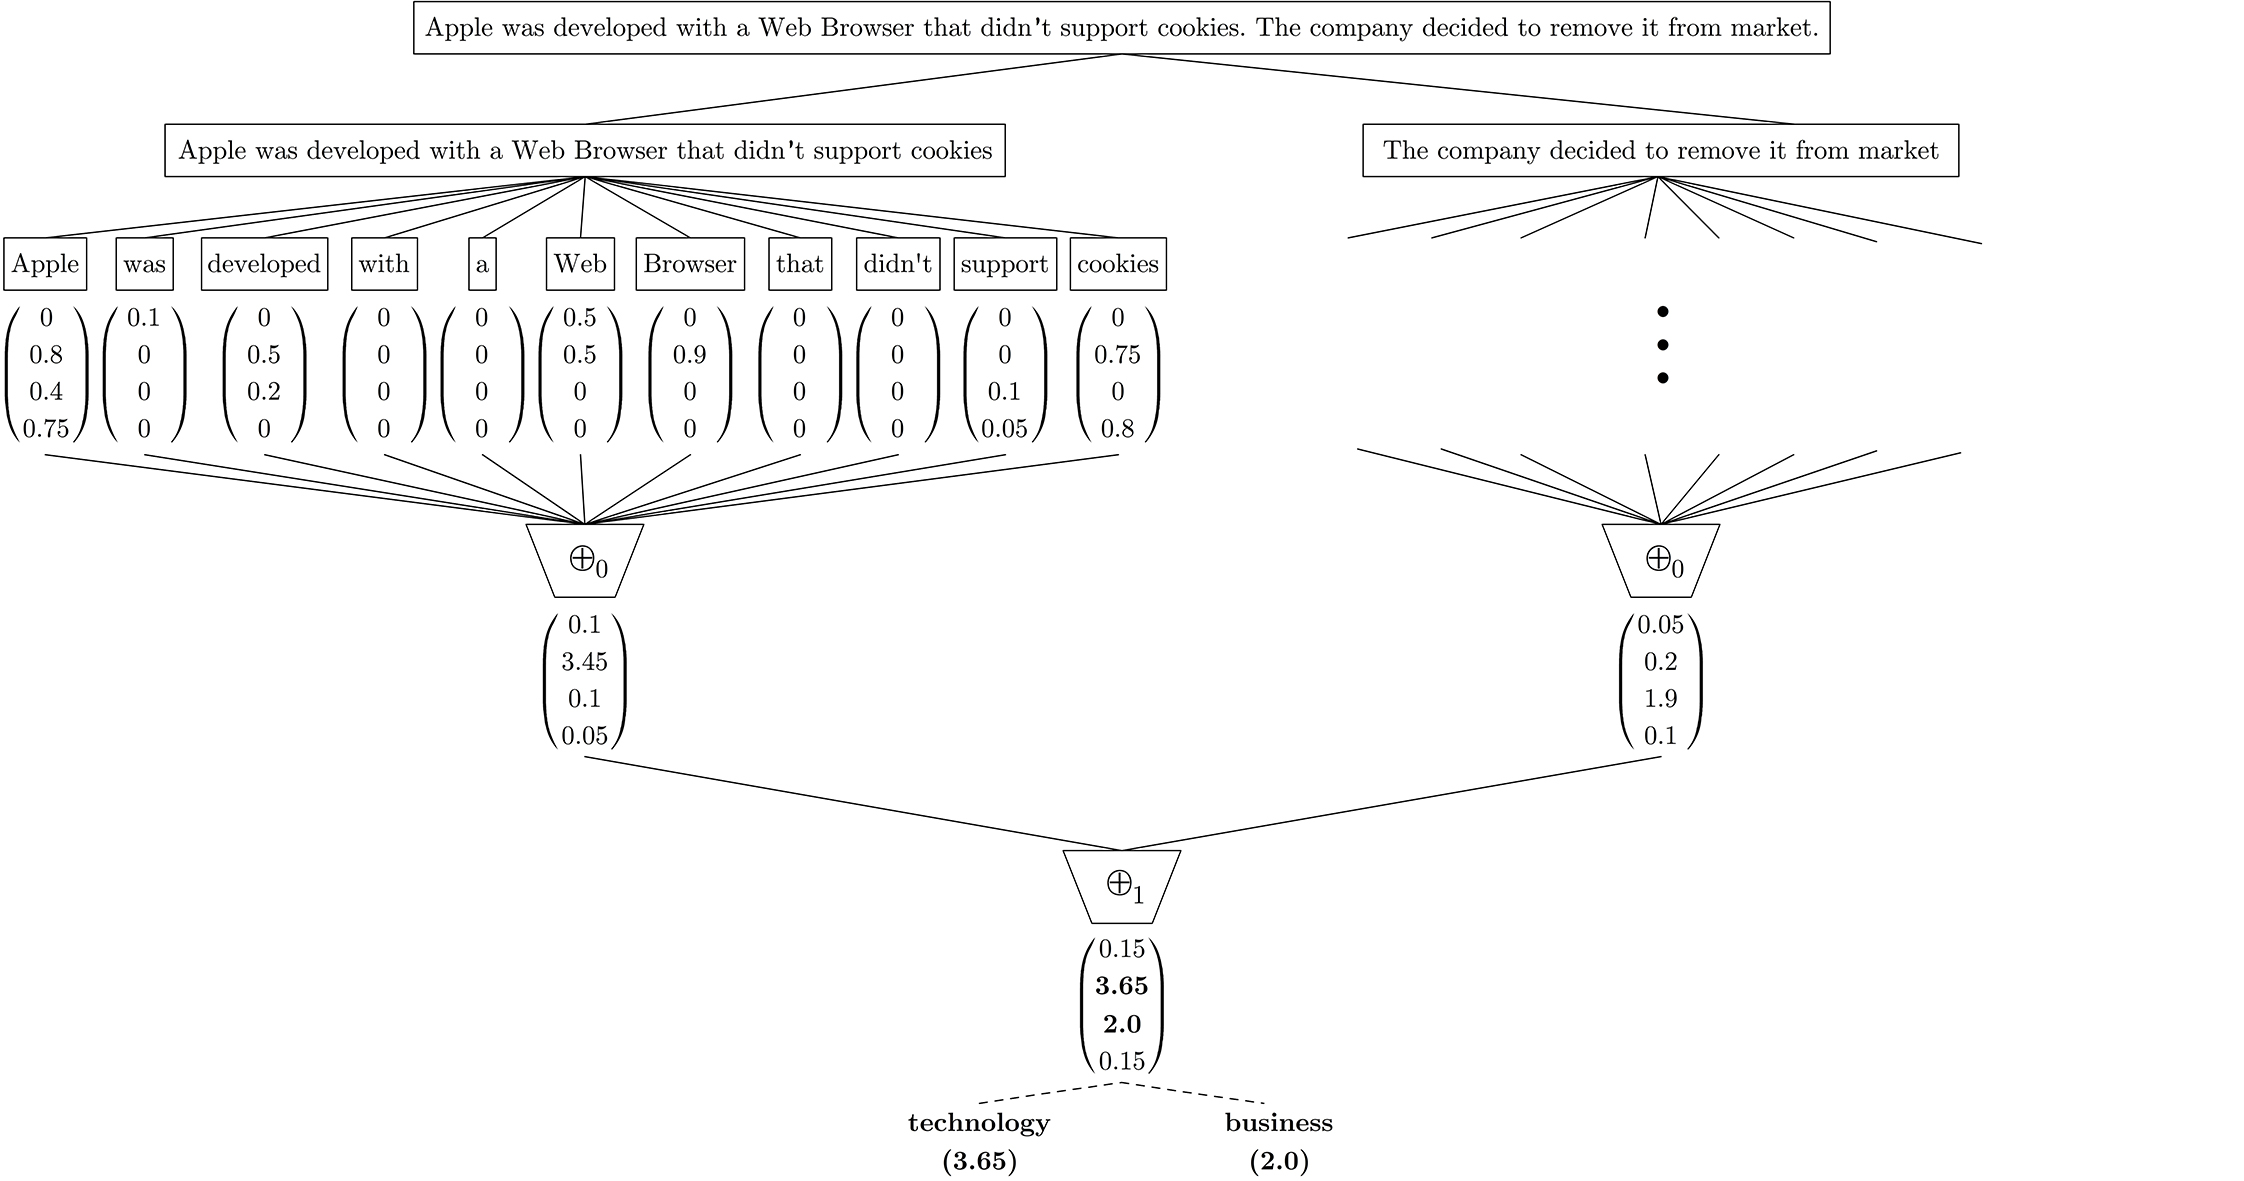
\includegraphics[width=190mm]{images/mapreduce-ss3}}
    \caption{Ejemplo del proceso de clasificación para el documento hipotético \emph{``Apple was developed with a Web Browser that didn't support cookies. The company decided to remove it from market''}.
    Al comienzo, este documento se divide en dos oraciones y luego cada oración a su vez se divide en palabras individuales.
    En este punto, se utiliza la función $gv$ sobre estas palabras individuales para obtener sus \emph{vectores de confianza}.
    Luego, estos vectores se reducen utilizando un operador especial, $\oplus_0$, a dos nuevos vectores de confianza a nivel oración, $\langle 0.1, 3.45, 0.1, 0.05\rangle$ y $\langle 0.05, 0.2, 1.9, 0.1\rangle$ para la primera y segunda oración, respectivamente.
    A su vez, estos dos últimos vectores también se reducen utilizando otro operador, $\oplus_1$, que en este caso es el operador de suma, a un único \emph{vector de confianza} final para todo el documento, $\langle 0.15, 3.65, 2.0, 0.15\rangle$.
    Finalmente, utilizando alguna política sobre este vector de confianza final, se selecciona la o las clases a ser signadas; en este ejemplo, se selecciona a \emph{tecnología} (\emph{technology}), por tener el valor de confianza más alto, y también a \emph{negocios} (\emph{business}) porque su valor está ``lo suficientemente cerca'' al de \emph{tecnología}.}
    % \caption{Classification process for a hypothetical example document ``Apple was developed with a Web Browser that didn't support cookies. The company decided to remove it from the market''.
% In the first stage, this document is split into two sentences (for instance, by using the dot as a delimiter) and then each sentence is also split into single words.
% In the second stage,  \emph{global values} are computed for every word to generate the first set of \emph{confidence vectors}.
% Then all of these word vectors are reduced by the $\oplus_0$ operator to sentence vectors, $(0.1, 3.45, 0.1, 0.05)$ and $(0.05, 0.2, 1.9, 0.1)$ for the first and second sentence respectively.
% After that, these two sentence vectors are also reduced by another operator ($\oplus_1$, which in this case is the addition operator) to a single \emph{confidence vector} for the entire document, $(0.15, 3.65, 2.0, 0.15)$.
% Finally, a policy is applied to this vector to make the classification ---which in this example was to select \emph{technology}, the category with the highest value, and also \emph{business} because its value was ``close enough'' to \emph{technology}'s.}
    \label{fig:mapreduce}
\end{figure*}


\

Ahora que ya hemos introducido los elementos y terminología necesaria, estamos listos para describir el proceso de clasificación, el cual puede pensarse como un proceso de dos fases, ilustrado con un ejemplo en la \autoref{fig:mapreduce}.
La primera fase comienza dividiendo el documento de entrada en múltiples bloques, luego cada bloque a su vez se divide sucesivamente en unidades más pequeñas hasta llegar a las palabras individuales.\footnote{Utilizaremos palabras aquí para simplificar la explicación, pero como se vio en la \autoref{sec:tipo-termino}, en principio se podría utilizar cualquier tipo de término, dependiendo de la tarea a resolver.} ---\emph{e.g.} dividir el documento en párrafos, párrafos en oraciones y oraciones en palabras.
Al finalizar esta fase, la entrada, previamente ``plana'', se ha convertido en una jerarquía de distintos niveles de bloques.
Así, diremos que las palabras están en el nivel 0 de la jerarquía, las oraciones en el nivel 1, los párrafos en el nivel 2, y así sucesivamente.
En la segunda fase, la función $gv$ se aplica a cada palabra para obtener los \emph{vectores de confianza} de ``nivel 0'', los cuales serán luego reducidos a \emph{vectores de confianza} de un siguiente nivel utilizando un operador especial para cada nivel, llamado \emph{operador de resumen}, $\oplus_0$.
Este proceso de reducción por operadores de resumen se propaga recursivamente a los bloques de nivel superior, hasta obtener un único \emph{vector de confianza} para toda la entrada.
Finalmente, la clasificación propiamente dicha se realiza aplicando alguna política para seleccionar las o la clase adecuada en base a los valores de este único \emph{vector de confianza} ---por ejemplo, seleccionando la clase con el máximo valor.
Notar que los \emph{operadores de resumen}, $\oplus_j$, se denotan utilizando un subíndice $j$, esto indica que cada nivel podría utilizar una operación diferente ---\emph{e.g.} $\oplus_0$ podría ser una suma de vectores, $\oplus_1$ el promedio (\emph{mean pooling}), $\oplus_2$ el máximo (\emph{max pooling}), y así. Más aún, no sólo operadores simples sino cualquier método, algoritmo o función, de la forma $f:2^{\mathbb{R}^n}\mapsto\mathbb{R}^n$, podría usarse como un \emph{operador de resumen}.
% Now that the needed basic definitions and terminology have been introduced, we are ready to describe the overall classification process, which is illustrated with an example in \autoref{fig:mapreduce}.
% Classification can be thought of as a 2-phase process.
% The first phase starts out by splitting the given input (usually a single document) into multiple blocks, then each block is in turn repeatedly divided into smaller units until words are reached.
% At the end of this phase, we have converted the previously ``flat'' input into a hierarchy of blocks.
% In practice, a document will be typically divided into paragraphs, paragraphs into sentences and sentences into words.
% Additionally, we will say that words are at level 0 in this hierarchy, sentences at level 1, paragraphs at level 2, and so on.
% In the second phase, the $gv$ function is applied to each word to obtain the level 0 \emph{confidence vectors}, which then are reduced by means of a \emph{summary operator} to generate the next level's \emph{confidence vectors}.
% This reduction process is recursively propagated up to higher-level blocks until a single \emph{confidence vector} is generated for the whole input.
% Finally, the actual classification is performed based on the values of this single \emph{confidence vector} ---some policy must be used, e.g. the category with the maximum value.
% Note that in the example shown in \autoref{fig:mapreduce}, \emph{summary operators} are denoted by $\oplus_j$, where $j$ denotes the level, to highlight the fact that each level (e.g. words, sentences, etc.) could have a different \emph{summary operator}
% ---for instance, $\oplus_0$ could be addition, $\oplus_1$ maximum (i.e. max pooling), $\oplus_2$ average (i.e. mean pooling), etc. Moreover, any function of the form $f:2^{\mathbb{R}^n}\mapsto\mathbb{R}^n$ could be used as a \emph{summary operator}.


\begin{figure}[t!] % [t]op; [h]ere; [p]age; [b]ottom; [r]ight; [l]eft
    \centering
    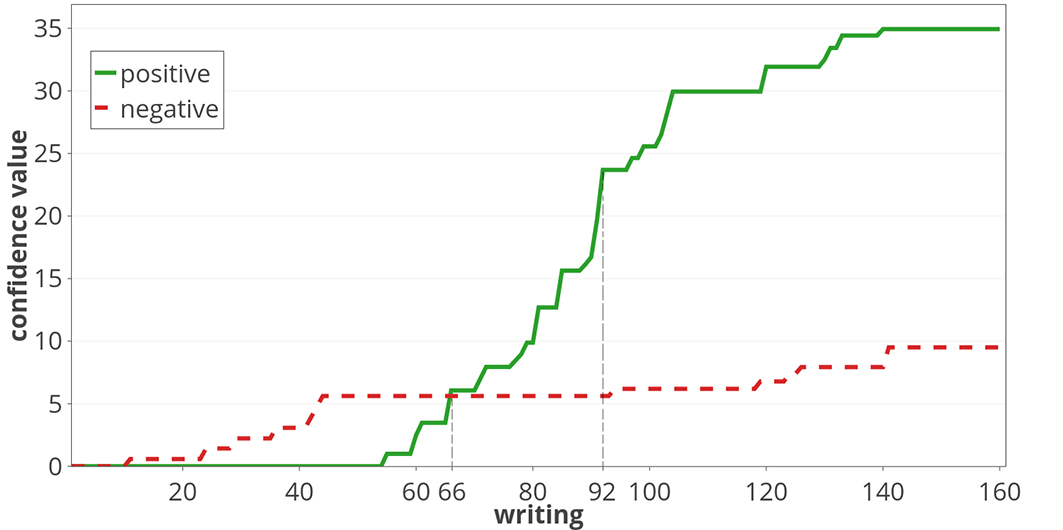
\includegraphics[width=120mm]{images/test_subject9579_writings}
    \caption{Variación del \emph{valor de confianza} positivo y negativo a lo largo del tiempo, hasta el momento. El tiempo se mide en publicaciones (writings) por lo que el gráfico seguiría creciendo a medida que el usuario escriba nuevas publicaciones.}
    % \caption{subject 9579's positive and negative confidence value variation over time. Time is measured in writings and it could be further expanded as more writings are created by the subject over time.}
    \label{fig:subject9579_writings}
\end{figure}

Vale la pena mencionar que este proceso le permite al clasificador explicar, visualmente, las razones detrás de la clasificación si, por ejemplo, en el documento de entrada se colorea cada bloque con una intensidad proporcional a su respectivo valor de confianza ---como se ilustrará con un ejemplo al final de la \autoref{sec:analysisAndDiscussion}.
Además, el clasificador podrá trabajar incrementalmente siempre que el \emph{operador de resumen} elegido para el último nivel pueda calcularse incrementalmente
---como es el caso con las operaciones de agregación más comunes, como la suma, la multiplicación, el máximo o incluso el promedio.\footnote{En el caso del promedio, sería necesario almacenar, además de la suma de los \emph{vectores de confianza} leídos hasta el momento, el número de vectores leídos.}
Por ejemplo, supongamos que más adelante se agrega una nueva oración al ejemplo mostrado en la \autoref{fig:mapreduce}, como $\oplus_1$ es la suma de vectores, en lugar de procesar nuevamente todo el documento, sólo necesitaríamos procesar la nueva oración para sumar su \emph{vector de confianza} a nuestro antiguo vector ya calculado, $\langle 0.15, 3.65, 2.0, 0.15\rangle$ ---obteniendo así el mismo vector final que obtendríamos si procesáramos toda la entrada nuevamente.
% It is worth mentioning that with this simple mechanism it would be fairly straightforward to justify when needed, the reasons of the classification by using the values of \emph{confidence vectors} in the hierarchy, as will be illustrated with a visual example at the end of \autoref{sec:analysisAndDiscussion}.
% Additionally, the classification is also incremental as long as the \emph{summary operator} for the highest level can be computed in an incremental fashion
% ---which is the case for most common aggregation operations such as addition, multiplication, maximum or even average.\footnote{In case of average it would be necessary to store, in addition to a vector with the sum of all previous \emph{confidence vectors}, their number.}
% For instance, suppose that later on, a new sentence is appended to the example shown in \autoref{fig:mapreduce}.
% Since $\oplus_1$ is the addition, instead of processing the whole document again, we could update the already computed vector, $(0.15, 3.65, 2.0, 0.15)$, by adding it to the new sentence \emph{confidence vector}
% --- Note that this incremental classification, in which only the new sentence needs to be processed, would produce exactly the same result as if the process were applied to the whole document again each time.
Finalmente, otro aspecto importante de este enfoque incremental es que, dado que este \emph{vector de confianza} final mantiene un resumen de la entrada leída hasta el momento, realizar un seguimiento de \emph{cómo} este vector cambia con el tiempo, a medida que se procesen nuevos elementos, debería permitirnos derivar reglas sencillas y claras para decidir \emph{cuándo} el clasificador puede hacer una clasificación anticipada.
% Another important aspect of this incremental approach is that since this \emph{confidence vector} is a value that ``summarizes the past history'', keeping track of \emph{how} this vector changes over time should allow us to derive simple and clear rules to decide \emph{when} the system should make an early classification. %, as we will see in section \autoref{sec:analysisAndDiscussion}.
Por ejemplo, supongamos que necesitamos clasificar a un usuario de una red social como ``positivo'' o ``negativo'' en relación a algún riesgo,  en base a las publicaciones que va generando.
Además, supongamos que este usuario efectivamente está en riesgo y que el cambio de los valores de su \emph{vector de confianza} hasta el momento, y a lo largo del tiempo, es el mostrado en la \autoref{fig:subject9579_writings}.
% As an example of this, suppose we need to classify a social media user (i.e. a subject) as depressed (positive) or non-depressed (negative) based on his/her writings.
% Let us assume that this user is the subject 9579, he/she is depressed, and that the change of each \emph{confidence vector} component over time (measured in writings) is the one shown in \autoref{fig:subject9579_writings}.
Podríamos hacer uso de esta información temporal y dinámica para diseñar políticas que le permitan al clasificador decidir en qué momento clasificar a los sujetos como positivos.
Por ejemplo, una política podría ser ``clasificar al usuario como positivo cuando el valor positivo actual sea mayor al negativo'', en cuyo caso nuestro usuario se hubiera clasificado como positivo luego de que éste escribiese su publicación número 66.
Otra política, un poco más elaborada, podría tener en cuenta qué tan rápido crece el valor positivo en relación al negativo, clasificando al usuario como positivo cuando el crecimiento supere cierto umbral. Por ejemplo, con una política de este tipo, nuestro usuario podría haber sido clasificado como positivo luego de haber escrito su publicación número 92.
% Tenga en cuenta que también se podrían combinar múltiples políticas como veremos en la \autoref{sec:analysisAndDiscussion}.
% We could make use of this ``dynamic information'' to apply certain policies to decide when to classify subjects as depressed.
% For example, one of such a policy would be ``classify a subject as positive when the accumulated positive value becomes greater than the negative one'' ---in which case, note that our subject would be classified as depressed after reading his/her 66th writing.
% Another (more elaborated) policy could have taken into account how fast the positive value grows (the slope) in relation with the negative one, and if a given threshold was exceeded, classify subjects as depressed ---in such case our subject could have been classified as depressed, for instance, after reading his/her 92nd writing.
% Note that we could also combine multiple policies as we will see in \autoref{sec:analysisAndDiscussion}.



\subsubsection{Entrenamiento}
\label{sec:training_process}

En la subsección anterior se describió el proceso de clasificación, el cual se apoya sobre los \emph{vectores de confianza}, los que a su vez se generan inicialmente con la función $gv$, la cual nos da el \emph{valor global} de las palabras.
En esta sección se describe cómo se lleva a cabo el entrenamiento del clasificador, esto es, cómo hace SS3 para aprender el \emph{valor global} de las palabras (\emph{i.e.} aprende a calcular $gv(w,c)$) en base a los documentos del conjunto de entrenamiento.
Sin embargo, el cálculo efectivo de $gv(w,c)$ se pospondrá para la \autoref{sec:local_global_value}, ya que, como se verá allí, SS3 puede calcularlo completamente conociendo la frecuencia de cada palabra.

De este modo, el entrenamiento propiamente dicho se vuelve trivial, ya que sólo consiste en almacenar la frecuencia total que tiene cada palabra dentro de cada clase.
% puede calcularse completamente en base a la frecuencia de cada palabra en cada clase, el entrenamiento de modelos SS3 es prácticamente trivial ya que sólo necesitaríamos almacenar dichas frecuencias.
Esto es, el algoritmo de aprendizaje simplemente consiste en la utilización de un diccionario de pares palabra-frecuencia por cada clase, para almacenar dichas frecuencias, y la posterior actualización de los mismos, a medida que se leen nuevos documentos de entrenamiento ---\emph{i.e} las palabras nuevas se agregan al diccionario y las ya conocidas actualizan su frecuencia.
% This brief subsection describes the training process, which is trivial. Only a dictionary of term-frequency pairs is needed for each category.
% Then, during training, dictionaries are updated as new documents are processed ---i.e. unseen terms are added and frequencies of already seen terms are updated.

\vspace{5mm}

Notar que con este simple algoritmo de entrenamiento, SS3 no necesita almacenar todos los documentos ni volver a entrenar desde cero cada vez que se agregan nuevos documentos de entrenamiento, en su lugar, sólo se deben actualizar las frecuencias ya almacenadas utilizando los nuevos documentos disponibles.
En otras palabras, el entrenamiento también puede realizarse incrementalmente,\footnote{En principio, incluso hasta nuevas clases podrían agregarse dinámicamente.} lo que dentro del área del aprendizaje automático se conoce como \emph{online learning}.
% Note that with this simple training method there is no need neither to store all documents nor to re-train from scratch every time a new training document is added, making the training incremental.\footnote{Even new categories could be dynamically added.}
Además, no es necesario, como es usual, crear y calcular una matriz documento-término, ya que, en particular, el concepto de documento deja de tener sentido para el modelo y, en su lugar, cada clase es vista como una ``gran bolsa de palabras''.
%Esto a su vez, como sugieren los resultados experimentales, dota al modelo de cierta robustez ante el conocido problema de desbalance de clases ---ya que el número de documentos en cada clase es irrelevante en tanto la frecuencia relativa de las palabras dentro de ``cada bolsa'' sea representativa.
% , durante la clasificación, $gv$ puede calcularse dinámicamente en función de las frecuencias almacenadas en los diccionarios ---aunque, en caso de que sea necesario, siempre será posible crearla.
Finalmente, desde un punto de vista computacional, el costo del entrenamiento es muy bajo, ya que sólo involucra actualizar las frecuencias de cada término, es decir, sólo involucra operaciones de suma.
% Additionally, there is no need to compute the document-term matrix because, during classification, $gv$ can be dynamically computed based on the frequencies stored in the dictionaries ---although, in case we are working in an offline fashion and to speed up classification, it is still possible to create the document-term matrix holding the $gv$ value for each term.
% Finally, also note that training computation is very cheap since involves only updating term frequencies i.e only one addition operation is needed.


\subsection{Detalles Técnicos y Formalización}
\label{sec:formal_description}

En esta sección se formalizan las descripciones e intuiciones introducidas en las secciones anteriores, brindando los algoritmos correspondientes y examinando el cálculo efectivo de $gv$.
% This section presents more formally the general and intuitive description given in the previous section.

\subsubsection{Algoritmos de Clasificación y Entrenamiento}
% \subsection{Classification and Training}

\begin{algorithm}[t!]
\small
\caption{\small Algoritmo de clasificación de SS3.
$MAX\_NIVEL$ es una constante que almacena el nivel máximo de jerarquía utilizado al particionar la entrada. Por ejemplo, debería usarse $MAX\_NIVEL=3$ cuando se trabaje con la partición ``párrafo- oración-palabra''.
La función \textproc{Map} aplica \textproc{Clasificar-a-Nivel}($bloque$, $n-1$) a cada $bloque$ en $bloques$ y devuelve la lista de vectores resultantes.
La función \textproc{Reduce} reduce los vectores en $bloques\_vcs$ a un solo vector utilizando el \emph{operador de resumen} $\oplus_{n-1}$}
\label{alg:classification}
\begin{algorithmic}
\Statex
\Function{Clasificar}{$texto$} \Returns un conjunto de etiquetas de clases
	\State \Input $texto$, una secuencia de símbolos
	\State \LocalVariables $\overrightarrow{c}$, el \emph{vector de confianza} del documento
	\State
	\State $\overrightarrow{c} \gets$ \Call{Clasificar-a-Nivel}{$texto$, $MAX\_NIVEL$}
	\State
	\State \Return una o más clases seleccionadas en base a $\overrightarrow{c}$ según alguna política
\EndFunction
\Statex \hrulefill
\Function{Clasificar-a-Nivel}{$texto$, $n$} \Returns un \emph{vector de confianza}
	\State \Input $texto$, una secuencia de símbolos
	\State \LocalVariables $bloques$, una lista de bloques de texto
	\State \localvarsindent $bloques\_vcs$, lista de \emph{valores de confianza} de los bloques
	\State
	\If{$n$ == 0} \Comment es decir, si $texto$ es ``indivisible'' (\emph{e.g.} $texto=$ una palabra)
		\State \Return $gv(texto)$
% 		\State \Return \Call{Valor-Global}{$texto$}
	\Else
		\State $bloques \gets$ dividir $texto$ en bloques más pequeños \Comment \emph{i.e.} en bloques de nivel $n$
		\State $bloques\_vcs \gets$ \Call{Map}{}(\Call{Clasificar-a-Nivel}{}, $bloques$, $n - 1$)
		\State \Return \Call{Reduce}{}(\Call{$\oplus_{n-1}$}{}, $bloques\_vcs$)
	\EndIf
\EndFunction
\end{algorithmic}
\end{algorithm}

En el \autoref{alg:classification} se presenta el algoritmo de clasificación general que lleva a cabo el proceso ilustrado anteriormente en la \autoref{sec:classification_process}.
% In \autoref{alg:classification} is shown the general multi-label classification algorithm which carries out the process illustrated earlier in \autoref{sec:classification_process}.
Notar que este algoritmo se puede paralelizar masivamente, ya que sigue de manera natural el modelo de programación \emph{MapReduce}~\cite{dean2008} para \emph{big data}, lo que, en principio, le daría al modelo la capacidad de procesar y manejar efectivamente grandes volúmenes de datos.
% Note that this algorithm can be massively parallelized since it naturally follows the Big Data programming model \emph{MapReduce}~\cite{dean2008}, giving the framework the capability of effectively processing very large volumes of data. 

\begin{algorithm}[t!]
\small
\caption{\small Algoritmo de entrenamiento de SS3, implementado aquí por el procedimiento \textproc{Aprender}, el cual puede volverse a ejecutar cuando nuevos documentos de entrenamiento se vuelvan disponibles.}
\label{alg:training}
\begin{algorithmic}
\Statex
\Procedure{Aprender}{$documentos$}
	\State \Input $documentos$, una lista de documentos etiquetados con su respectiva clase
	\State
	\For{$documento$ \In $documentos$}
		\State \Call{Aprender-Documento}{$documento$.TEXTO, $documento$.ETIQUETA}
	\EndFor
	\State
	\State \Call{Actualizar-Valores-Globales}{}() \Comment{este paso es opcional}
\EndProcedure
\Statex \hrulefill
\Procedure{Aprender-Documento}{$texto$, \emph{etiqueta}}
	\State \Input $texto$, la secuencia de palabras del documento
	\State \inputindent \emph{etiqueta}, la etiqueta de la clase a la que pertenece el documento
	\State
	\State DICCIONARIO $\gets$ el diccionario correspondiente a la clase de la \emph{etiqueta}
	\For{\emph{palabra} \In $texto$}
		\If{\emph{palabra} $\notin$ DICCIONARIO}
			\State agregar \emph{palabra} a DICCIONARIO
		\EndIf
		\State DICCIONARIO[\emph{palabra}] $\gets$ DICCIONARIO[\emph{palabra}]$ + 1$
	\EndFor
\EndProcedure
\end{algorithmic}
\end{algorithm}

En el \autoref{alg:training} se presenta el algoritmo de entrenamiento descrito informalmente en la sección anterior.
Notar que la línea que llama a la función \textproc{Actualizar-Valores-Globales}, la cual calcularía y actualizaría todos los valores globales dados por $gv$, sólo sería necesaria si quisiéramos precomputarlos y almacenarlos a modo de caché, por ejemplo, para evitar recalcularlos reiteradas veces durante la clasificación;
% In \autoref{alg:training} is shown the training process described earlier.
% Note that the line calling the \textproc{Actualizar-Valores-Globales} function, which calculates and updates all global values, is only needed if we want to construct the document-term matrix to work in the standard batch-like way.
de lo contrario, puede omitirse ya que, como mencionamos, durante la clasificación $gv$ podría calcularse dinámicamente en función de las frecuencias almacenadas en los diccionarios.
Finalmente, vale la pena mencionar que este algoritmo también podría paralelizarse siguiendo el modelo \emph{MapReduce} ---por ejemplo, el conjunto de entrenamiento podría dividirse en lotes, luego paralelamente se calculan las frecuencias dentro de cada lote y, finalmente, todas estas frecuencias locales se sumarían para obtener las frecuencias totales.
% Otherwise, it can be omitted since, during classification, $gv$ can be dynamically computed based on the frequencies stored in the dictionaries.
% It is worth mentioning that this algorithm could be easily parallelized by following the MapReduce model as well ---for instance, all training documents could be split into batches, then frequencies locally calculated within each batch, and finally, all these local frequencies summed up to obtain the total frequencies.


\subsubsection{Valor Global de una Palabra}
% \subsection{Local and Global Value of a Word}
\label{sec:local_global_value}

En esta sección finalmente abordaremos cómo podría hacer SS3 para aprender, efectivamente, el \emph{valor global} de las palabras en base a los documentos de entrenamiento.
% En otras palabras, abordamos cómo sería posible calcular $gv(w,c)$ en base a las frecuencias almacenadas durante el entrenamiento.
No obstante, y antes de comenzar, es necesario recordar que se espera que el modelo final sea confiable y transparente, capaz de explicar las razones detrás de la clasificación, como se explicó en la \autoref{sec:EC}.
Por lo tanto, SS3 debe ser interpretable para, de este modo, poder proveer explicaciones completamente fieles a lo que el modelo realmente computa\footnote{En tareas de riesgo, no es recomendable utilizar modelos de caja negra, no interpretables, ya que éstos requieren de técnicas especiales (tales como LIME, SHAP, Mean Decrease Accuracy o DeepLIFT) para generar las explicaciones. Dado que dichas explicaciones sólo brindan una \emph{aproximación} del funcionamiento real del modelo, su uso puede, entre otros problemas, ser peligroso~\cite{rudin2019stop}}.
Más precisamente, para que SS3 sea interpretable, se necesita que la valoración de las palabras por medio de este \emph{valor global} sea interpretable.
Sin embargo, uno de los principales desafíos de la interpretabilidad es que, dado que  pueden haber diferentes ideas de lo que constituye interpretabilidad, es necesario definirla de una manera específica al dominio abordado para luego integrar dicha definición directamente dentro de nuestro modelo~\cite{rudin2019stop}. 
Por lo tanto, es necesario definir qué constituya la interpretabilidad en el dominio abordado en este trabajo, esto es, la clasificación de texto para la DAR.

En la DAR, se espera que las explicaciones sean interpretables no para el científico computacional sino para un público no especializado ---por ejemplo, para un experto en la problemática abordada, como ser un especialista en la salud mental.
Así, en este trabajo, diremos que un modelo es interpretable si es capaz de valorar a las palabras de una forma que sea intuitiva para una público general, no especializado en las ciencias computacionales.
Más específicamente, inspirados en la forma en la que una persona típicamente le explicaría a otra en base a qué palabras decidió clasificar a un texto de cierta manera,\footnote{Por ejemplo, uno esperaría que la persona dirija su atención sólo a ciertas palabras, que funcionarían como ``palabras clave'', ignorando así la gran mayoría de las demás.} esperaremos que el modelo aprenda por un lado a identificar y valorar, con diferencia, a ciertas ``palabras clave'', y por el otro, filtrar todas las palabras que no sean necesarias, asignándole un valor casi nula a todas ellas ---similar a lo ejemplificado al comienzo de la \autoref{sec:classification_process}.
Por este motivo, no es posible utilizar un esquema de pesado de términos convencional, como ser \emph{tf-idf}, \emph{BM25} score, o los basados en \emph{DFR}, entre otros, ya que, en resumen, necesitamos una valoración que cumpla con estos dos requisitos: (a) que pondere cada término en relación a la decisión final, esto es, en relación a cada clase, no a cada documento;\footnote{Notar que los pesados de términos tradicionales fueron pensados para construir \emph{representaciones} de documentos, por lo que valoran un término en relación a un documento dado, no a una clase en particular.} y además (b) que dicha ponderación sea interpretable en el sentido ya mencionado.
De hecho, no conocemos un esquema de pesado que sea capaz de satisfacer estos dos aspectos en simultaneo, por lo que, en lo que resta de esta sección abordamos cómo sería posible calcular el \emph{valor global} de una palabra para lograrlo.
Esto es, desarrollaremos y propondremos una serie de ecuaciones para calcular $gv(w, c)$, en base a las frecuencias almacenadas durante el entrenamiento, intentando cumplir con ambos requerimientos.

\

Nuestro enfoque para calcular el \emph{valor global} busca superar los problemas que surgen de valorar las palabras únicamente basándonos en información local a cada clase. Para ello, primeramente, por medio de una función $lv(w,c)$ valoraremos la palabra únicamente en base a información local a cada clase, llamando a este valor como \emph{valor local}, pero luego combinaremos estos valores locales para obtener así el \emph{valor global} de la palabra, $gv(w,c)$.
% Our approach to calculating $gv$, as we will see later, tries to overcome some problems arising from the valuation of words only based on local information to a category. This is carried out by, firstly, computing a word \emph{local value} ($lv$) for every category, and secondly, combining them to obtain the \emph{global value} of the word in relation to all the categories.
Así, lo lógico es que el \emph{valor local} de una palabra $w$ en una clase $c$ sea proporcional a la probabilidad de que dicha palabra ocurra en textos de dicha clase, esto es, $lv$ debería ser alguna función tal que $lv(w, c)\propto P(w|c)$. Por lo tanto, definiremos a $lv$ como:
% More precisely, the \emph{local value} should be a function such that $lv(w, c) \propto P(w|c)$ i.e. the \emph{local value} of $w$ in $c$ should be proportional to the probability of $w$ occurring, given the category $c$. Therefore, $lv$ will be defined by:


\begin{equation}
\label{eq:lv-first}
lv(w, c) = \frac{P(w|c)}{P(w_{max}|c)}
\end{equation}


Donde $w_{max}$ denota la palabra más probable en la categoría $c$.
Notar que en lugar de definir $lv$ simplemente como $lv(w, c) = P(w|c)$, hemos decidido dividir dicha probabilidad por la probabilidad de la palabra más probable.
Esto produce dos efectos deseables:
(a) $lv$ está normalizado y la palabra más probable tendrá un valor de $1$ y, más importante aún,
(b) cada palabra se valora en relación a qué tan cerca esté su valor al de la más probable.
Lo interesante de este último punto es que las o la palabra más probable no dependerá de una clase en particular, sino del lenguaje en sí mismo. De hecho, en la práctica, la palabra más probable siempre será alguna de las \emph{palabras vacías} (tal como ``el'', ``la'', ``los'', ``las'', etc.) ya que por definición son palabras altamente frecuentes y cuya frecuencia está dada por el rol que desempeñan dentro del lenguaje en sí mismo, sin referir a la realidad extralingüística particular de cada clase.
Notar que con este simple ``truco'' de normalización, absolutamente todas las palabras se valoran en relación a un único elemento global e independiente de las clases particulares ---\emph{i.e.} las \emph{palabras vacías}. En otras palabras, hemos habilitado la posibilidad de \emph{comparar el valor local de una misma palabra a lo largo de las diferentes clases en ``igualdad de condiciones''} ---lo que en última instancia nos permitirá calcular su valor global.
% \footnote{Puede suceder que no sea exactamente la misma palabra para todas las clases, pero de ser ese el caso, serán \emph{palabras vacías} igualmente frecuentes, lo que a fines prácticos producirá los mismos resultados.}
%De hecho, en distintos experimentos realizados, la palabra más probable en todas las clases muy habitualmente resultó ser la palabra más frecuente del idioma inglés, ``the'', aunque para algunas clases, por ejemplo, resultaron ser ``be'', ``to'' o ``of'', la segunda, tercera o cuarta más frecuente del idioma.
% Notar que esto nos permite comparar el valor de una misma palabra a lo largo de las diferentes clases dado que su valor local en cada clase estará normalizado en relación a alguna \emph{palabra vacía}, las cuales siempre tendrán una probabilidad similar ya que su frecuencia está dada por el rol que desempeñan dentro del lenguaje en sí mismo, sin referir a la realidad extralingüística de cada clase en particular.
%, en gran medida, por la naturaleza propia del lenguaje en cuestión (Español, Inglés, etc.), y no por una clase en sí.
% Note that this allows us to compare words across different categories since their values are all normalized in relation to stop words, which should have a similar frequency across all the categories.\footnote{Note that we are assuming here that we are working with textual information in which there exist highly frequent elements that naturally have similar frequency across all categories (e.g. such as stop words).}

Sin embargo, antes de continuar con el cálculo del valor global, definiremos a $lv$ de una forma más general, ya que la definición dada en la \autoref{eq:lv-first} supone que la proporción $lv(w, c) \propto P(w|c)$ es directa, lo que no necesariamente tiene que cumplirse siempre. Así, agregaremos un parámetro, $\sigma$, que nos permitirá regular, de cierto modo, qué tan directa es la proporción $lv(w, c) \propto P(w|c)$, de la siguiente manera:
% However, our current definition of $lv$ implicitly assumes that the proportionality $lv(w, c) \propto P(w|c)$ is direct, which is not always true so we will define $lv$ more generally as follows:

$$lv_\sigma(w, c) = \left(\frac{P(w|c)}{P(w_{max}|c)}\right)^\sigma$$

\vspace{5mm}

Lo cual, después de estimar las probabilidades mediante \emph{estimación por máxima verosimilitud} (EMV) analítica, nos lleva finalmente a la siguiente definición, en términos de las frecuencias aprendidas durante el entrenamiento:
% Which, after estimating the probability, $P$, by an analytical \emph{Maximum Likelihood Estimation}(MLE) derivation, leads us to the actual definition:

\vspace{5mm}

\begin{equation}
\label{eq:lv-fr}
lv_\sigma(w, c) = \left(\frac{fr_{w,c}}{max\{fr_c\}}\right)^\sigma
\end{equation}

\vspace{5mm}

Donde $fr_{w, c}$ denota la frecuencia de $w$ en $c$ y $max\{fr_c\}$ la máxima frecuencia vista en $c$. De esta forma, el valor $\sigma\in(0, 1]$ es el primer hiperparámetro de nuestro modelo, denominado como ``suavidad'', y cuyo papel es doble ya que nos permite:
% Where $tf_{w,c}$ denotes the frequency of $w$ in $c$ and $max\{tf_c\}$ the maximum frequency seen in $c$. The value $\sigma  \in (0, 1]$ is the first hyper-parameter of our model, called ``smoothness'', and whose role is twofold:
\begin{itemize}
    \item Controlar qué tan rápido crecerá el \emph{valor local} de una palabra en relación a qué tan cerca esté su frecuencia a la de la más probable ---\emph{e.g.} cuando $\sigma = 1$, el crecimiento será lineal. %proporcional a $P(w|c)$.
    % \item Control how fast grows the \emph{local value} of a word in relation to how close it is to the most probable one; e.g. when $\sigma=1$, $lv$ grows linearly proportional to $P(w|c)$.
    \item Controlar ``la suavidad'' de la distribución de las palabras, que de lo contrario, según la ley empírica de Zipf \cite{zipf1949human, powers1998applications}, tendrá un grupo extremadamente pequeño de palabras muy frecuentes eclipsando a las importantes.
    % \item Control the smoothness of the distribution of words which otherwise, by the empirical Zipf's law \cite{zipf1949human, powers1998applications}, will have a very small group of highly frequent words overshadowing important ones.
\end{itemize}

\begin{figure}[t]
    \begin{subfigure}{0.5\textwidth}
        \centering
        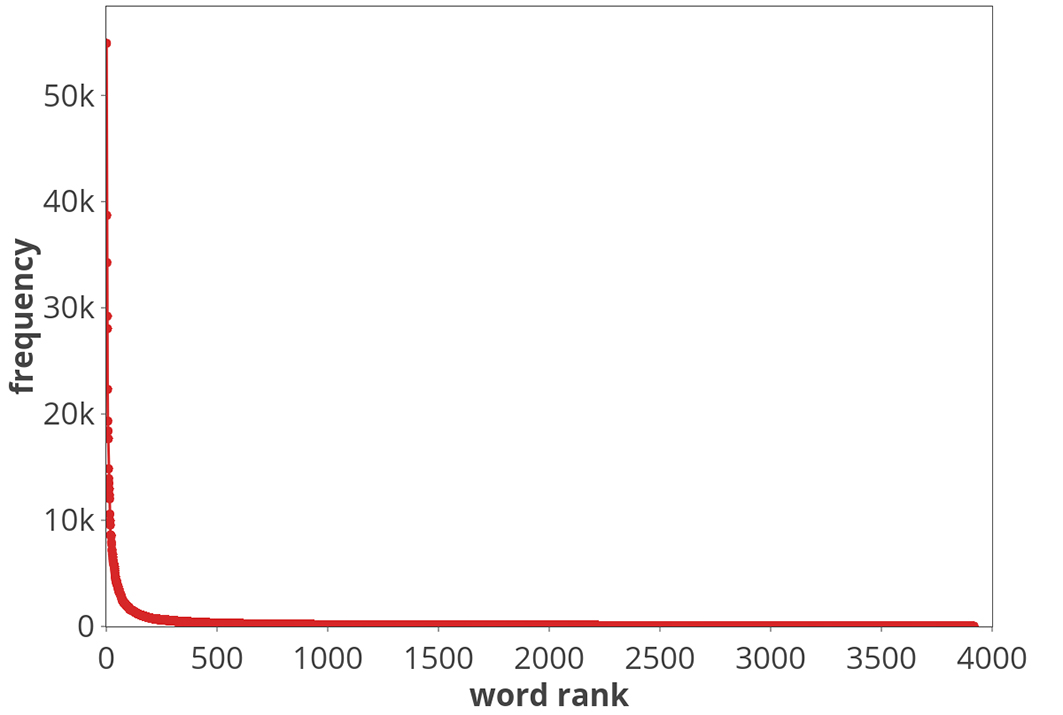
\includegraphics[width=90mm]{images/word-fr}
        \caption{}
        \label{fig:sigma_a}
    \end{subfigure}
    \begin{subfigure}{0.5\textwidth}
        \centering
        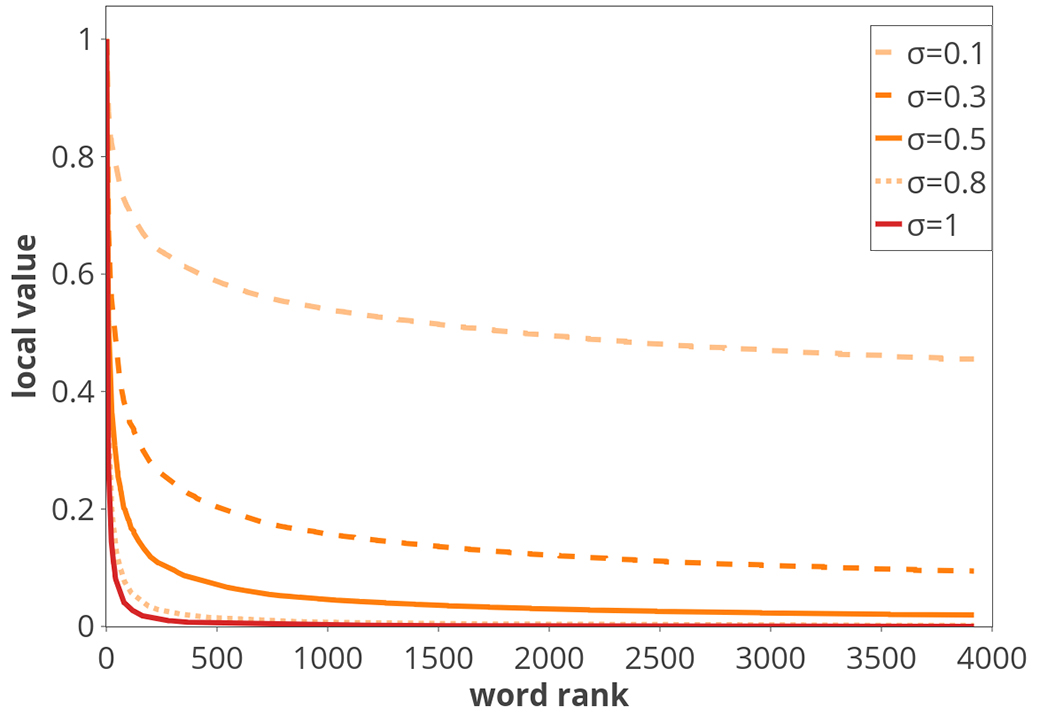
\includegraphics[width=90mm]{images/sigmas}
        \caption{}
    \end{subfigure}
\caption{
    (a) Curva con la distribución de la frecuencia de las palabras.
    (b) Curva con la distribución del \emph{valor local} de las palabras para cinco valores distintos de $\sigma$: $1$, $0.8$, $0.5$, $0.3$ y $0.1$.
    Las abscisas representan el ranking de las palabras individuales ordenadas por frecuencia en (a) y por valor local en (b).
    Notar que cuando $\sigma = 1$ (línea roja en (b)), la distribución de los \emph{valores locales} coincide exactamente, en forma, con la distribución de las frecuencias en bruto en (a). Sin embargo, a medida que el valor de $\sigma$ disminuye, la curva ``se suaviza'', haciendo que la brecha entre los valores más altos y más bajos se reduzca.
    % word-\emph{local value} diagram for 5 different values of $\sigma$: 1, 0.8, 0.5, 0.3 and 0.1.
    % The abscissa represents individual words arranged in order of frequency.
    % Note that when $\sigma=1$, $lv_1$ (red line) matches the shape of the raw frequency (the actual word distribution), however, as $\sigma$ decreases, the curve becomes smoother; reducing the gap between the highest and the lowest values.
}
\label{fig:sigma}
\end{figure}

Ambos aspectos se ilustran con un ejemplo en la \autoref{fig:sigma}.\footnote{En la práctica, normalmente los valores de $\sigma$ que nos han producido mejores resultados son los cercanos a $0.5$, lo que equivaldría, aproximadamente, a aplicarle la raíz cuadrada a la \autoref{eq:lv-first}.}
% These two items are illustrated with an example in \autoref{fig:sigma} ---a good value for $\sigma$ should be around 0.5, which would be approximately equivalent to taking the square root of the \autoref{eq:lv-first}.

\vspace{5mm}

Ahora que hemos definido una forma para calcular el \emph{valor local} de una palabra en las distintas clases, estamos listos para definir cómo combinar dichos valores para obtener su \emph{valor global}. Así, de forma general, definiremos a $gv(w,c)$ como $lv(w,c)$ regularizado por dos pesos especiales que capturan información global, $sig$ y $san$ , del siguiente modo:
% Now that we are able to compute word \emph{local values}, we are going to define its \emph{global value} based on them, as follows:

\begin{equation}
gv(w, c) = lv_\sigma(w, c)\times sig_{\lambda}(w, c)\times san_\rho(w, c)
\label{eq:gv}
\end{equation}

Donde $\lambda, \rho \in \mathbb{R}^+$ son los otros dos hiperparámetros del modelo, referidos como ``significancia'' y ``sanción'' respectivamente, y donde $sig$ y $san$ son dos funciones que, consultando el valor local de esa misma palabra $w$ en las otras clases, resaltarán o disminuirán su valor local en la clase dada $c$.
Más precisamente, $sig$ debería intentar capturar la ``significancia'' o importancia que tiene $w$ en $c$ observando su valor local en las otras clases, mientras que $san$ debería sancionar el valor final de $w$ en relación al número de clases para las cuales finalmente resultó importante, según $sig$.
% Where $sg$ and $sn$ are functions of the form $f:W\times C\mapsto [0, 1]$.
% As we will see, the former decreases $lv$ in relation to the global significance of $w$, and the latter sanctions it, in relation to the number of categories for which $w$ is significant.
% Additionally, the values  $\lambda, \rho \in \mathbb{R}^+$ referred to as ``significance'' and ``sanction'' respectively, are the other two hyper-parameters of our model.

\vspace{5mm}

De este modo, para que $sig(w, c)$ pueda reflejar correctamente la importancia de una palabra, $w$, con respecto a una clase, $c$, debería ser alguna función tal que:
(a) devuelva un valor cercano a $1$ cuando $lv(w, c)$ sea significativamente mayor que $lv(w, c_i)$ para las otras clases $c_i$; y a la inversa,
(b) devuelva un valor cercano a $0$ cuando sus \emph{valores locales} en las distintas clases sean similares entre sí, esto es, cuando $lv(w, c_i)$ sea similar para las distintas clases $c_i$.
Por ejemplo, $lv(\text{\emph{`el'}},c_i)$ será similarmente alto para todas las clases $c_i$, mientras que $lv(\text{\emph{`pan'}}, \text{alimentos})$ será probablemente mayor que $lv(\text{\emph{`pan'}}, c_i)$ para la mayoría de las otras clases; por lo tanto, $sig(\text{\emph{`el'}},c_i)$ debería devolvernos un valor cercano a $0$ mientras que $sig(\text{\emph{`pan'}}, \text{alimentos})$ cercano a $1$.
En general, podríamos modelar este comportamiento utilizando cualquier función sigmoide:
% In order to represent the significance of a word, $w$, with respect to a category, $c$, $sg(w, c)$ should be a function such that:
% (a) it outputs a value close to 1 when $lv(w, c)$ is significantly greater than $lv(w, c_i)$, for most other categories $c_i$; and
% (b) it outputs a value close to 0 when all $lv(w, c_i)$ are close to each other, for all $c_i$.
% For instance, $lv($`$the$'$, c_i)$ probably will be a similarly large value for all categories $c_i$, whereas $lv($`$bread$'$, food)$ probably will be greater than most  $lv($`$bread$'$, c_i)$, for other categories; hence $sg($`$the$'$, c_i)$ should be close to 0 and $sg($`$bread$'$, food)$ close to 1.
% In general, we could model this behavior by using any sigmoid function, as follows:


$$sig_{\lambda}(w, c) = sigmoide\left(lv(w, c) - \widetilde{LV}_w, \ \lambda\times MAD_w\right)$$

Tal que:
\begin{enumerate}
    \item[(I)] $sigmoide(d, l)\approx 1$ si $d\geq l$; y
    \item[(II)] $sigmoide(d, l)\approx 0$ si $d\leq0$.
\end{enumerate}

Donde $LV_w = \{lv(w, c_i) | c_i\in C\}$, es decir, el conjunto con todos los  \emph{valores locales} de $w$ en las distintas clases;
$\widetilde{LV}_w$ denota la mediana de $LV$;
$MAD_w = mediana(|lv(w,c_i)-\widetilde{LV}_w|)$, es decir, la \emph{Desviación Mediana Absoluta}\footnote{MAD, del inglés, Median Absolute Deviation.} de $LV_w$.
% Where $LV_w = \{lv(w, c_i) | c_i\in C\}$ i.e. the set of all \emph{local values} of $w$;
% $\widetilde{LV}_w$ denotes the median of $LV$;
% $MAD_w = median(|lv(w,c_i)-\widetilde{LV}_w|)$ i.e. the \emph{Median Absolute Deviation} of $LV_w$.
Notar que el hiperparámetro $\lambda$
% \footnote{si $\lambda$ es aproximadamente cercano a $1.4826$, entonces $\lambda\cdot MAD_w$ es aproximadamente igual a la \emph{desviación estándar} de $LV_w$, por lo tanto, $\lambda\approx 3\times1.4826$ podría ser un buen valor inicial para $\lambda$, siempre que $LV_w$ tenga una distribución normal.}
% Additionally, note that the hyper-parameter $\lambda$\footnote{
    % if $\lambda$ is approximately close to 1.4826, then $\lambda\cdot MAD_w$ is approximately equal to the \emph{standard deviation} of $LV_w$, thus perhaps setting $\lambda \approx 3\times1.4826$ would be a good value, as long as $LV_w$ has a normal distribution
% }
nos permite controlar qué tanto debe desviarse el \emph{valor local} de la mediana de \emph{valores locales} para ser considerado como significativo, es decir, mientras más cerca esté $lv(w, c)-\widetilde{LV}_w$ de superar a $\lambda\cdot MAD_w$, más cerca estará esta función $sigmoide$ de $1$.
% controls how far the \emph{local value} must deviate from the median to be considered significant i.e. the closer $lv(w, c)-\widetilde{LV}_w$ to $\lambda\cdot MAD_w$, the closer the $sigmoid$ to 1, and therefore, also the closer $sg_{\lambda}(w, c)$ to 1 ---which is the desired behavior.

Así, en particular, y sin perdida de generalidad, utilizaremos a la función sigmoide $tanh$ para definir a $sig$ como se definió arriba, cumpliendo con las propiedades allí mencionadas, del siguiente modo:
% In particular, we have decided to use $tanh$ as the $sigmoid$ function, hence $sg$ is defined by:

\begin{equation}
    sig_{\lambda}(w, c) = \frac{1}{2}\times tanh\left(4\times\frac{lv(w, c) - \widetilde{LV}_w}{\lambda\times MAD_w} - 2\right) + \frac{1}{2}
\end{equation}

\vspace{5mm}

Finalmente, necesitamos definir a $san$, la función de sanción, que disminuirá proporcionalmente el \emph{valor global} de una palabra en relación al número de clases para las cuales es significativa, según $sig$. Por lo tanto, $san$ debería ser una función tal que: (a) cuando $w$ sea significativo para una sola clase $c$, \emph{i.e.} cuando $sig_{\lambda} (w, c)\approx 1$ para un único $c$,  $san(w , c)$ debe ser igual a $1$; (b) cuanto mayor sea el número de clases en las que $w$ es significativa, menor debe ser el valor de $san(w, c)$. Por lo tanto, sin pérdida de generalidad, definiremos a $san$ como:
% Finally, we need to define $sn$, the sanction function, which will proportionally decrease the \emph{global value} of $w$, in relation to the number of categories for which $w$ is significant. Hence $sn$ should be a function such that: (a) when $w$ is significant (i.e. $sg_{\lambda}(w, c) \approx 1$) to only one category $c$, $sn(w, c)$ should be equal to 1; (b) the greater the  number of categories $w$ is significant to, the lower the value of $sn(w, c)$. Therefore, we have defined $sn$ by:

\begin{equation}
\label{eq:san}
    san_\rho(w, c) = \left(\frac
        {|C| - \left(\hat{C}_{wc} + 1\right)}
        {\left(|C|-1\right)\left(\hat{C}_{wc} + 1\right)}
    \right)^\rho
\end{equation}

% \begin{equation}
% \label{eq:san}
%     san_\rho(w, c) = \left(-\frac
%         {\hat{C}_{wc}}
%         {|C|-1} + 1
%     \right)^\rho
% \end{equation}

% \begin{equation}
% \label{eq:san}
%     san_\rho(w, c) = \left(-\frac
%         {\hat{C}_{wc}}
%         {|C|-1} + 1
%     \right)^\rho
% \end{equation}


Donde $|C|$ denota el número de clases y, 
$$\hat{C}_{wc} = \sum_{c_i\in C-\{c\}}sig_{\lambda}(w, c_i)$$
% Where $|C|$ denotes the number of categories and,
% $$\hat{C}_{wc} = \sum_{c_i\in C-\{c\}}sg_{\lambda}(w, c_i)$$


En palabras, $\hat{C}_{wc}$ es igual a la suma de ``la importancia'' de $w$ en todas las clases excepto $c$.
Notar que la \autoref{eq:san} se comporta de la manera deseada, por ejemplo,
cuando $w$ sea significativo para casi todas las clases, tendremos que $\hat{C}_{wc}\approx |C|-1$, y por lo tanto $san(w, c)\approx 0$, mientras que cuando $w$ sea significativo para una sola clase, $c$, se tendrá que $\hat{C}_{wc} = 0$, y por lo tanto $san(w, c) = 1$.
% i.e. $\hat{C}_{wc}$ is equal to the summation of $sg_{\lambda}(w, c_i)$ for all categories in $C$ except $c$.
% Note that, for instance, when extreme cases are met, \autoref{eq:san} behaves properly;
% namely, when $w$ is significant to almost all categories, $\hat{C}_{wc}\approx |C|-1$, and thus $sn(w, c)\approx 0$;
% and when $w$ is significant to only one category, $c$, $\hat{C}_{wc} = 0$, and thus $sn(w, c)= 1$.
Finalmente, notar que el hiperparámetro $\rho$ nos permite controlar qué tan severa es la sanción en relación al número de clases para las cuales la palabra es significativa.
% The hyper-parameter $\rho$ controls how severe the sanction is, in proportion to the number of significant categories.\footnote{
%     setting $\rho\approx 1$ probably is a good starting point, although we can adjust this value in relation to how overlapped categories are.
% }

\vspace{5mm}

Antes de concluir con esta sección, creemos conveniente introducir un ejemplo sencillo para ilustrar cómo el \emph{valor global} puede interpretarse efectivamente, según lo hemos definido en la \autoref{eq:gv}, como un porcentaje de su \emph{valor local} ($lv$), dado por su importancia ($sig$) y una sanción regularizadora ($san$). Así, supongamos que se tienen las siguientes tres clases $C=\{\text{\emph{alimentos}}, \text{\emph{tecnología}}, \text{\emph{negocios}}\}$, luego:
% To conclude this section, let us introduce a simple example to illustrate how the \emph{global value} is a percentage of its \emph{local value} given by its significance ($sg$) and sanction ($sn$). Suppose we have the following three categories $C = \{f, t, b\}$ for $food$, $tech$, and $business$ respectively, then:

\begin{itemize}
    \item {
        Para las \emph{palabras vacías} tendríamos, siendo $c$ cualquiera de las clases, casos similares al siguiente:
        % For stopwords, like `the', we would have, regardless of the category $c\in C$, something like:

        \vspace{5mm}

        \begin{tabular}{l@{}l}%p{0.5\linewidth}}
            $gv($`$el$'$, c)$  & $= lv($`$el$'$, c)\times sig($`$el$'$, c)\times san($`$el$'$, c)$\\
                            & $= lv($`$el$'$, c)\times 0.05\times 1$\\
                            & $= lv($`$el$'$, c)\times 0.05$\\
                            & $= 0.92\times 0.05 = 0.04$
        \end{tabular}

        \vspace{5mm}

        Notar que si bien el \emph{valor local} de ``el'' es alto ($0.92$), su \emph{valor global} final resultó ser muy bajo ($0.04$), sólo un $5\%$ de su \emph{valor local}.
        Esto se debe al hecho de que el \emph{valor local} de ``el'' fue igualmente alto en todas las clases y, por lo tanto, según definición de $sig$, su importancia es cercana a nula ---en este caso, $sig($`$el$'$, c) = 0.05$. A su vez, como su importancia es nula en todas las clases, no se aplicó ninguna sanción ---$san($`$el$'$, c)=1$.
        % While the \emph{local value} of `the' is 0.92, its final \emph{global value} turned out to be 0.04 (5\% of its \emph{local value}).
        % This is due to the fact that $lv($`$the$'$, c)$ is similarly high for all categories, and by definition, the significance function should be close to 0 ---in this case, $sg($`$the$'$, c)= 0.05$.
    }
    \vspace{5mm}
    \item {
        Para palabras que sean principalmente significativas para una única clase, como podría ser, por ejemplo, `pan' para \emph{alimentos}, tendríamos casos similares a éste:
        % For a word that is mainly significant to a single category, in this case, `bread' to food, we would have something like:

        \vspace{5mm}
        
        \begin{tabular}{l@{}l}%p{0.5\linewidth}}
            $gv($`$pan$'$, \text{\emph{alimentos}})$ & $= lv($`$pan$'$, \text{\emph{alimentos}})\times sig($`$pan$'$, \text{\emph{alimentos}})$\\ 
            					& \ \ \ $\times san($`$pan$'$, \text{\emph{alimentos}})$\\
                                & $= lv($`$pan$'$, \text{\emph{alimentos}})\times 0.99\times 0.95$\\
                                & $= lv($`$pan$'$, \text{\emph{alimentos}})\times 0.94$\\
                                & $= 0.65\times 0.94 = 0.61$
        \end{tabular}
        
        \vspace{5mm}

        El \emph{valor global} terminó siendo casi idéntico a su \emph{valor local} ---siendo más exactos, un $94\%$ de éste. Esto se debe a que no sólo la palabra fue significativa para \emph{alimentos} ($ sig($`$pan$'$, \text{\emph{alimentos}})=0.99$), sino que, además, prácticamente no se le aplicó ninguna sanción ($san($`$pan$'$, \text{\emph{alimentos}})=0.95$) debido a que no fue significativa para casi ninguna otra clase.
        % The \emph{global value} is almost identical to its \emph{local value} (about 94\%). This is due to the word being significant ($sg\approx 1$) \emph{only} to food ($sn\approx 1$).
    }
    \vspace{5mm}
    \item {
        Para palabras que son significativas para más de una clase, tendríamos casos similares al siguiente:
        % For a word that is significant to more than a single category, we would have something like:

        \vspace{5mm}

        \begin{tabular}{l@{}l}%p{0.5\linewidth}}
            $gv($`$apple$'$, \text{\emph{tecnología}})$ & $= lv($`$apple$'$, \text{\emph{tecnología}})\times sig($`$apple$'$, \text{\emph{tecnología}})$\\
            					& \ \ \ $\times san($`$apple$'$, \text{\emph{tecnología}})$\\
                                & $= lv($`$apple$'$, \text{\emph{tecnología}})\times 0.85\times 0.6$\\
                                & $= lv($`$apple$'$, \text{\emph{tecnología}})\times 0.51$\\
                                & $= 0.7\times 0.51 = 0.35$
        \end{tabular}
        
        \vspace{5mm}

        En este caso, el \emph{valor global} terminó siendo un $51\%$ de su \emph{valor local}.
        Notar que si bien ``apple'' es bastante significativa para \emph{tecnología} ($sig($`$apple$'$, \text{\emph{tecnología}})=0.85$), también lo debe ser para alguna o algunas de las otras dos clases, \emph{alimentos} y/o \emph{negocios}, al menos en cierta medida, porque fue moderadamente sancionado ($san($`$apple$'$, \text{\emph{tecnología}})=0.6$).
        % In this case, the \emph{global value} ended up being about 51\% of its \emph{local value}.
        % Note that while `apple' is quite significant to $tech$ ($sg=0.85$), it must also be significant to some of the other categories, at least to a certain degree, because it is being moderately sanctioned ($sn=0.6$).
    }
\end{itemize}

Es interesante notar que SS3 aprenderá a ignorar las \emph{palabras vacías} automáticamente, ya que para ellas tendremos, por definición, que $gv(w, c)\approx0$, por lo que no necesitaríamos eliminarlas manualmente durante el preprocesamiento, como es habitual.
% It is worth mentioning that SS3 will learn to automatically ignore stop words since, by definition, $gv(w, c)\approx0$ for all of them.
% Therefore, there is no need to manually remove stop words.
De hecho, la eliminación de las \emph{palabras vacías} probablemente produzca un efecto negativo ya que, como se explicó luego de definir la \autoref{eq:lv-fr}, la valoración de todas las palabras se realiza, precisamente, usando a las \emph{palabras vacías} como punto común independiente de clases particulares ---lo que nos permite compararlas a lo largo de las distintas clases para obtener sus valores globales.
% Moreover, stop words removal could cause negative effects since in \autoref{eq:lv} we are implicitly evaluating words in terms of stop words.\footnote{\textcolor{blue}{That is, words are normalized over the frequency of the most probable one, which will always be a stop word.
% Note that the fact that stop words have a similar distribution across all the categories enables us to compute the $gv$ value of a word by comparing its $lv$ value across different categories.}}
No obstante, no hay nada en el modelo que nos impida utilizar cualquier otra técnica de preprocesamiento, tales como \emph{stemming} o \emph{lemmatization}.
% However, there is nothing in the model preventing us from using any other type of preprocessing, such as stemming, lemmatization, etc.

\

Finalmente, también es interesante mencionar que el clasificador \acf{MNB} puede verse como ``una instancia posible'' del modelo SS3. En concreto, una instancia en la que el valor global se redujera simplemente al valor local, definiendo a $gv$ como $gv(w, c) = lv(w, c) = log\ P(w|c)$ y a $\oplus_j = suma$, para todo $j$.\footnote{Al final de la \autoref{sec:mnb} del \autoref{cap2} se explicó la razón de este $log\ P(w|c)$ en \ac{MNB}.}
Sin embargo, esta instancia de SS3 no cumpliría efectivamente nuestros objetivos, ya que,
% A saber, como se tiene que $\sum_{w \in W} P(w|c) = 1$ por definición de probabilidad $P$, esto es, la suma de las probabilidades de todas las palabras deben ser 1, y dado que el número de palabras por clase es generalmente muy grande, los distintos valores $log\ P (w|c)$ terminan siendo extremadamente pequeños y muy similares entre sí (esto último debido al efecto del logaritmo) sin importar la palabras $w$.
de esta manera, la frecuencia local de una palabra en una clase pasaría a ser el único factor que determinase su valor. Así, ``palabra frecuente'' se volvería sinónimo de ``palabra valiosa'' y, por lo tanto, las palabras realmente valiosas se verían ocultas por simples palabras frecuentes, pero sin importancia ---como las \emph{palabras vacías}.
% Esto afecta tanto a la capacidad de describir qué palabras ayudaron a tomar la decisión como así también, por lo general, al desempeño del modelo ---otros tipos de modelos, tales como \ac{SVM} habitualmente superan a \ac{MNB}.
En resumen, el principal aspecto negativo con \ac{MNB} radica en el hecho de que las palabras se valoran sólo y exclusivamente en base a información local a cada clase, siendo precisamente éste el problema que el cálculo de $gv(w,c)$ intenta resolver.
% It is interesting to notice that Multinomial Naive Bayes can be seen as one possible instance of the SS3 framework. Namely, when $gv(w,c) = lv(w,c) = log\ P(w|c)$ and $\oplus_j = addition$, for all $j$.
% However, this instance of SS3 would not effectively fulfill our goals.
% Since we have $\sum_{w\in W}P(w|c) = 1$ by definition of $P$, i.e. the probabilities of all words must sum up to 1, and since the number of words per category is usually very large, $log\ P(w|c)$ is usually very small and very similar (due to the effect of using $log$) for all the words, $w$.
% Additionally, important words would be overshadowed by unimportant (or less important), but highly frequent, words such as stop words.
% This disfavors both the power to describe what words helped to make the decision and usually the performance as well---other types of models, such as SVM, frequently outperform MNB.
% The main issue with MNB arises from the fact that terms are valued simply and solely by their local raw frequency. In short, that is basically the problem that $gv$ computation tries to overcome.



\section{Evaluación Experimental}
\label{sec:exp}

En esta sección se cubrirá el análisis experimental del modelo propuesto, abordando la tarea de detección anticipada de depresión.
La siguiente subsección describe brevemente la tarea y el conjunto de datos utilizado para entrenar y probar los distintos modelos.
En la \autoref{sec:eval_metric} se introduce la medida de desempeño utilizada para evaluar la efectividad de los clasificadores teniendo en cuenta tanto el desempeño en la clasificación como también su demora.
Finalmente, la \autoref{sec:exp_and_results} describe los diferentes tipos de experimentos realizados y los resultados obtenidos.
% In this section, we cover the experimental analysis of SS3, the proposed approach.
% The next subsection briefly describes the pilot task and the dataset used to train and test the classifiers.
% In \autoref{sec:eval_metric} we will introduce the time-aware metric used to evaluate the effectiveness of the classifiers, in relation to the time taken to make the decision. Finally, \autoref{sec:exp_and_results} describes the different types of experiments carried out and the obtained results.


\subsection{Conjunto de Datos y Tarea Piloto}
\label{sec:data_sets}

\begin{table*}[t]
\centering
\caption{Estadísticas principales del conjunto de datos de la tarea.}
\label{tab:dataset}
\begin{tabular}{l c c|c c}
\hline
& \multicolumn{2}{c}{Entrenamiento} & \multicolumn{2}{c}{Prueba}\\
& Depresivos & Control & Depresivos & Control \\ \hline
No. de sujetos & 83 & 403 & 52 & 349 \\
No. de publicaciones & 30851 & 264172 & 18706 & 217665 \\
Prom. de publicaciones por sujeto & 371.7 & 655.5 & 359.7 & 623.7 \\
Prom. de días (primera a última publ.) & 572.7 & 626.6 & 608.3 & 623.2 \\
Prom. de palabras por publicación & 27.6 & 21.3 & 26.9 & 22.5 \\ \hline

\hline
\end{tabular}
\end{table*}

% \begin{table*}[t]
% \centering
% \caption{Estadísticas principales del conjunto de datos de la tarea.}
% \label{tab:dataset-dep-2018}
% \begin{tabular}{l c c|c c}
% \hline
% & \multicolumn{2}{c}{Entrenamiento} & \multicolumn{2}{c}{Prueba}\\
% & Depresivos & Control & Depresivos & Control \\ \hline
% No. de sujetos & 135 & 752 & 79 & 741 \\
% No. de publicaciones & 49557 & 481837 & 40665 & 504523 \\
% Prom. de publicaciones por sujeto & 367.1 & 640.7 & 514.7 & 680.9 \\
% Prom. de días (primera a última publ.) & 586.43 & 625.0 & 786.9 & 702.5 \\
% Prom. de palabras por publicación & 27.4 & 21.8 & 27.6 & 23.7 \\ \hline

% \hline
% \end{tabular}
% \end{table*}

% \begin{table*}[t]
% \centering
% \caption{Estadísticas principales del conjunto de datos de la tarea.}
% \label{tab:dataset-ano-2018}
% \begin{tabular}{l c c|c c}
% \hline
% & \multicolumn{2}{c}{Entrenamiento} & \multicolumn{2}{c}{Prueba}\\
% & Anorexia & Control & Anorexia & Control \\ \hline
% No. de sujetos & 20 & 132 & 41 & 279 \\
% No. de publicaciones & 7452 & 77514 & 17422 & 151364 \\
% Prom. de publicaciones por sujeto & 372.6 & 587.2 & 424.9 & 542.5 \\
% Prom. de días (primera a última publ.) & 803.3 & 641.5 & 798.9 & 670.6 \\
% Prom. de palabras por publicación & 41.2 & 20.9 & 35.7 & 20.9 \\ \hline

% \hline
% \end{tabular}
% \end{table*}

Los experimentos se realizaron con la tarea piloto eRisk\footnote{\url{http://early.irlab.org/2017/task.html}} del CLEF 2017\footnote{\url{http://clef2017.clef-initiative.eu}} sobre \emph{detección anticipada de riesgo de depresión}.
% Experiments were conducted on the CLEF 2017\footnote{\url{http://clef2017.clef-initiative.eu}} eRisk pilot task\footnote{\url{http://early.irlab.org/2017/task.html}}, on \emph{early risk detection of depression}.
Esta tarea piloto se centró en el procesamiento secuencial del contenido publicado por un conjunto de usuarios en Reddit\footnote{\url{https://www.reddit.com}}.
El conjunto de datos utilizado en esta tarea, introducido inicialmente en Losada \emph{et al.} \cite{losada2016test}, es una colección, cronológicamente ordenada, de publicaciones de usuarios, los cuales son referidos en esta tarea como ``sujetos''.
Hay dos clases de sujetos en este conjunto de datos, \emph{``depresivos''} y \emph{``control''} (\emph{i.e.} ``no depresivos''), los primeros están compuestos por usuarios que mencionaron explícitamente que fueron diagnosticados con depresión, mientras que el segundo por usuarios aleatorios de la misma plataforma.
Además, como es habitual, para comparar los resultados entre los diferentes participantes, el conjunto de datos completo se dividió en dos subgrupos, un conjunto de entrenamiento y un conjunto de prueba.
Los detalles sobre estos conjuntos se brindan en la \autoref{tab:dataset}. Notar que los conjuntos están altamente desbalanceados, es decir, sólo están etiquetados como \emph{depresivos} el $17\%$ de los sujetos del conjunto de entrenamiento y el $12.9\%$ del conjunto de prueba.
% This pilot task focused on sequentially processing the content posted by users on Reddit\footnote{\url{https://www.reddit.com}}.
% The dataset used in this task, which was initially introduced and described in \cite{losada2016test}, is a collection of writings (submissions) posted by users; here users will also be referred to as ``subjects''.
% There are two categories of subjects in the dataset, \emph{depressed} and \emph{control} (non-depressed).
% Additionally, in order to compare the results among the different participants, the entire dataset was split into two sets: a training set and a test set.
% The details of the dataset are presented in \autoref{tab:dataset}. Note that the dataset is highly unbalanced, namely, only 17\% of the subjects in training set are labeled as \emph{depressed}, and 12.9\% in the test set.

Es importante tener en cuenta que, como se describe en la Sección 2.2 de Losada \emph{et al.} \cite{losada2016test}, para construir el conjunto con sujetos depresivos, los autores primero recolectaron usuarios haciendo búsquedas específicas en Reddit para obtener expresiones auto-reportadas de diagnósticos de depresión y, luego, revisaron manualmente las publicaciones coincidentes para verificar que fueran realmente genuinas.
Según los autores, esta revisión manual fue estricta, expresiones como ``tengo depresión'', ``creo que tengo depresión'' o ``estoy deprimido'' no calificaban como expresiones explícitas de un diagnóstico. Sólo incluían a un usuario en el grupo de depresión cuando hubiera una mención clara y explícita de un diagnóstico ---\emph{e.g.} ``en 2013, me diagnosticaron depresión'', ``después de luchar contra la depresión durante muchos años, ayer me diagnosticaron''. Notar que esto introduce la posibilidad de tener algunos falsos positivos en los datos recolectados, por lo tanto, en lo que resta de este trabajo la palabra ``depresivo'' debe interpretarse como ``posiblemente diagnosticado con depresión''.
% It is important to note that, as it is described in Section 2.2 of \cite{losada2016test}, to construct the depression group, authors first collected users by doing specific searches on Reddit (e.g. ``I was diagnosed with depression'') to obtain self-expressions of depression diagnoses, and then they manually reviewed the matched posts to verify that they were really genuine.
% According the authors, this manual review was strict, expressions like ``I have depression'', ``I think I have depression'', or ``I am depressed'' did not qualify as explicit expressions of a diagnosis. They only included a user into the depression group when there was a clear and explicit mention of a diagnosis (e.g., ``In 2013, I was diagnosed with depression'', ``After struggling with depression for many years, yesterday I was diagnosed''). That introduces the possibility of having some noise in both categories of the collected data, therefore, from now on, when we refer to ``depressed''  it should be interpreted as ``possibly diagnosed with depression''.

En esta tarea piloto, los clasificadores deben decidir, \emph{tan pronto como sea posible}, qué sujetos son depresivos en función de sus publicaciones.
Para llevar esto a cabo, durante la etapa de prueba y de acuerdo con la definición de la tarea piloto, el historial completo de publicaciones de cada sujeto se dividió en 10 \emph{bloques} ---por lo tanto, cada \emph{bloque} contenía el $10\%$ del total de sus publicaciones. Durante la prueba, a los clasificadores se les entregó el historial de publicaciones, un bloque a la vez, y, luego de cada entrega, se les pidió que decidieran si su autor era depresivo, no depresivo o si, de lo contrario, era necesario leer más bloques para tomar la decisión.
% In this pilot task, classifiers must decide, as \emph{early} as possible, whether each user is depressed or not based on his/her writings.
% In order to accomplish this, during the test stage and in accordance with the pilot task definition, the subject's writings were divided into 10 \emph{chunks} ---thus each \emph{chunk} contained 10\% of the user's history. Then, classifiers were given the user's history, one chunk at a time, and after each chunk submission, the classifiers were asked to decide whether the subject was depressed, not depressed or that more chunks need to be read.


\subsection{Medida de Evaluación}
\label{sec:eval_metric}

Las medidas de evaluación de desempeño convencionales para tareas de clasificación, como son $F_1$, \emph{precision} y \emph{recall},\footnote{Introducidas en la \autoref{sec:medidas} del \autoref{cap2}.} no tienen en cuenta ningún aspecto vinculado a la demora en la clasificación, ya que no son ``conscientes'' del tiempo.
Por esa razón, en la tarea piloto se utilizó una nueva medida de evaluación, introducida en Losada \emph{et al.} \cite{losada2016test}, llamada como medida \emph{ERDE}, del inglés \emph{Early Risk Detection Error}, la cual se define de la siguiente manera:
% Standard classification measures such as $F_1$-measure ($F_1$), Precision ($\pi$) and Recall ($\rho$) are time-unaware.
% For that reason, in the pilot task, the measure proposed in \cite{losada2016test} was also used, called \emph{Early Risk Detection Error} (ERDE) measure, which is defined by:



\begin{equation}
  ERDE_o(d,k) = \left\{
     \begin{array}{@{}l@{\thinspace}l}
        c_{fp} &\ si\ d=p\ y\ verdad=n\\
        c_{fn} &\ si\ d=n\ y\ verdad=p\\
        lc_o(k)\cdot c_{tp} &\ si\ d=p\ y\ verdad=p\\
        0 &\ si\ d=n\ y\ verdad=n\\
     \end{array}
   \right.
\label{eq:erde}
\end{equation}



Donde $lc_o(k)$, denominada como \emph{función de costo de latencia}, se define con la siguiente sigmoidal:
$$lc_o(k) = 1 - \frac{1}{1+e^{k - o}}$$

La demora se mide contando el número ($k$) de publicaciones vistas antes de tomar la decisión binaria ($d$) que podría ser positivo ($p$) o negativo ($n$).
Además, notar que la función sigmoidal $lc_o(k)$ está parametrizada por el parámetro $o$, el cual permite definir un ``tiempo límite'' para la toma de decisión ya que si se toma una decisión correcta positiva en un tiempo $k>o$, el costo de la latencia asignada por esta función será de $1$ y,\footnote{Estrictamente hablando, al ser una sigmoidal, este valor de penalización nunca será exactamente $0$ o $1$, sino asintóticamente cercano a $0$ o $1$, respectivamente.} por lo tanto, $ERDE_o$ la considerará como si hubiera sido incorrecta (falso positivo).
Así, la función de penalización, $lc_o(k)$, busca reflejar la naturaleza binaria de las tareas de detección de riesgo en donde, a diferencia de otras tareas de clasificación anticipada en las que el costo a pagar por una demora aumenta gradualmente con el tiempo, existe un punto específico en el tiempo que se intenta anticipar y que torna a cualquier clasificación posterior sin sentido.
Por ejemplo, en la \autoref{fig:lc50} se muestra esta \emph{función de costo de latencia} para $o=50$, notar que las decisiones tomadas en cualquier momento $k>50$ tendrán, rápidamente, una penalización máxima, es decir, un costo de latencia virtualmente igual a $1$.

\begin{figure}[t!]
    \centering
    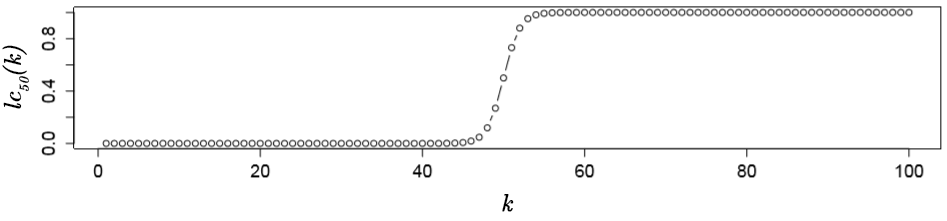
\includegraphics[width=\textwidth]{images/penalty-lc50}
    \caption{\emph{función de costo de latencia}, $lc_o(k)$, para $o=50$.}
\label{fig:lc50}
\end{figure}

De esta manera, la medida $ERDE_o$ acumulará error tanto cuando la clasificación sea incorrecta como cuando sea correcta pero habiéndose superado el umbral de decisión dado por $o$.
Por lo tanto, esta medida permite comparar el rendimiento de distintos modelos en relación a qué tan rápidos y efectivos sean ya que, mientras más rápido y más efectivo sea un modelo, más cercano a nulo será el error acumulado y, por lo tanto, más cercano a $0$ será su valor $ERDE_o$.\footnote{Como se verá en el \autoref{cap:eRisk2019}, esta medida no es perfecta, por ejemplo, si bien nos permitirá realizar comparaciones relativas entre modelos, su semántica en términos absolutos, sin contexto, no es tan clara (¿Qué significaría que el valor $ERDE_5$ obtenido sea de, por ejemplo, $11.31\%$?¿es el modelo rápido o lento?).
Por lo que, en dicho capítulo, se introducirá una medida adicional que buscará abordar algunos de estos aspectos.}
Además, el costo de una clasificación incorrecta no será igual cuando la decisión involucre a un usuario en riesgo que cuando no, ya que, en la práctica, se suele utilizar $c_{fn} \gg c_{fp}$ para reflejar el hecho de que cada usuario positivo no detectado (falso negativo) es una vida en riesgo y, en consecuencia, el costo a pagar en dicho caso es elevado ($c_{fn}$).\footnote{Además, esta elección ayuda a evitar la utilización de modelos triviales que clasifiquen a todos los usuarios como negativos.}

% Por ejemplo, si bien la medida $ERDE_o$ permite realizar comparaciones relativas entre modelos, su semántica en término de su valor absoluto no es tan clara.\footnote{¿Qué significa que el valor $ERDE_5$ obtenido haya sido de, por ejemplo, $11.31\%$?¿fue el modelo rápido o lento?}

%la medida $ERDE_o$ resaltará a los modelos que prioricen $recall$ por sobre $precision$,\footnote{Esto se debe a la forma en que se calcula la medida $ERDE_o$ (\autoref{eq:erde}), siendo el costo de los falsos positivos ($cfp$) considerablemente más pequeño que el de los falsos negativos ($cfn$).} lo que no es necesariamente malo teniendo en cuenta que se lidia con tareas de riesgo en donde cada usuario (positivo) no detectado es una vida en riesgo.

Finalmente, en la tarea piloto se utilizaron, específicamente, las medidas $ERDE_5$ y $ERDE_{50}$ y se fijaron los valores $c_{fn} = c_{tp} = 1$ y el valor $c_{fp}$ como el número de sujetos depresivos dividido por el total de sujetos en el conjunto de prueba, es decir, se fijó $c_{fp}= \frac{52}{401} = 0.129$.
%In order to avoid building trivial classifiers that always say no, we need to have $cfn >> cfp$





\subsection{Detalles de Implementación}
\label{sec:implementation}

El modelo propuesto fue codificado manualmente en \emph{Python 2.7} utilizando solamente funciones y estructuras de datos nativas, como ser \emph{dict} para los diccionarios o las funciones \emph{map} y \emph{reduce} para simular localmente el patrón \emph{MapReduce}.
Además, por simplicidad, se decidió utilizar la suma de vectores como implementación de los \emph{operadores de resumen}, $\oplus_j$, para todo nivel $j$.
Dado que este trabajo se centra en la detección anticipada, y no en aspectos vinculados al cómputo paralelo para clasificación a gran escala, no fue necesario realizar una implementación real del modelo de cómputo paralelo \emph{MapReduce}.
Además, implementar una versión \emph{MapReduce} no hubiera sido adecuada, ya que en la \autoref{subsec:exp-scenario2} analizamos el tiempo de cómputo de los clasificadores y todos ellos deben compartir el mismo tipo de implementación, sin paralelismo, para que la comparación sea justa.
Por el mismo motivo, todos los otros clasificadores utilizados en \autoref{subsec:exp-scenario2} fueron implementados con el paquete \emph{sklearn},\footnote{\url{https://scikit-learn.org/}} versión 0.17, también en \emph{Python 2.7}.
Además, para estos clasificadores se utilizó una representación de bolsa de palabras con pesado \emph{tf-idf}, por lo que la vectorización de la entrada se realizó con la clase \emph{TfidfVectorizer}. El preprocesamiento se llevó a cabo eliminando las palabras vacías\footnote{Utilizando la lista estándar de palabras vacías para el inglés.} y las palabras que tuvieran una frecuencia de documentos inferior a 20. Finalmente, estos clasificadores se implementaron utilizando sus correspondientes versiones ya integradas en \emph{sklearn}, tales como las clases \emph{LogisticRegression, KNeighborsClassifier}, o \emph{MultinomialNB}, entre otras.

% SS3 was manually coded in \emph{Python 2.7} using only built-in functions and data structures, e.g. a \emph{dict} to store the category's dictionary or \emph{map} and \emph{reduce} functions to (locally) simulate a \emph{MapReduce} pattern.
% Since this paper focuses on early detection, not computing nor large-scale classification, we did not perform a real \emph{MapReduce} implementation.
% Moreover, since in \autoref{subsec:exp-scenario2} we are also reporting the computation time taken by all the other classifiers and all of them must share the same type of implementation, implementing a \emph{MapReduce} version would not have been fair.
% Thus, all these other models were also implemented in \emph{Python 2.7}, using the \emph{sklearn} library\footnote{\href{https://scikit-learn.org/}{https://scikit-learn.org/}}, version 0.17. Vectorization was done with the \emph{TfidfVectorizer} class, with the standard English stop words list. Additionally, terms having a document frequency lower than 20 were ignored. Finally, classifiers were coded using their corresponding \emph{sklearn} built-in classes, e.g. \emph{LogisticRegression, KNeighborsClassifier, MultinomialNB}, etc.


\subsection{Experimentos y Resultados}
%\subsection{Comparison with Related work}
\label{sec:exp_and_results}

Esta subsección describe el trabajo experimental, el cual se llevó a cabo bajo dos escenarios diferentes.
En el primero, realizamos los experimentos de acuerdo con la definición original de la tarea piloto eRisk, utilizando los \emph{bloques} de publicaciones.
Sin embargo, dado que esta definición supone, mediante el uso de bloques, que el número total de publicaciones de cada usuario se conoce de antemano\footnote{Hecho que no se cumple en ambientes en  los que los usuarios generan contenido dinámicamente, tales como las redes sociales.}, decidimos considerar también un segundo tipo de experimento, uno que simule un escenario más realista en el que el historial de cada usuario sea procesado ``en flujo'', una publicación a la vez.
% This subsection describes the experimental work, which was divided into two different scenarios.
% In the first one, we performed experiments in accordance with the original eRisk pilot task definition, using the described \emph{chunks}.
% However, since this definition assumes, by using chunks, that the total number of user's writings is known in advance\footnote{Which is not true when working with a dynamic environment, such as Social Media.}, we decided to also consider a second type of experiment, simulating a more realistic scenario, in which user's history was processed in a streaming way, one writing (post) at a time.


\subsubsection{Escenario 1: clasificación incremental bloque a bloque (configuración original)} 

Como se tienen sólo dos clases con poco solapamiento entre ellas, decidimos fijar los hiperparámetros $\lambda$ y $\rho$ del modelo SS3 en $1$. De hecho, también realizamos algunas pruebas con otros valores que mejoraron la \emph{precision} o el \emph{recall} pero empeorando la medida \emph{ERDE}.
La optimización de hiperparámetros se realizó aplicando una \emph{búsqueda en grilla} sobre el hiperparámetro $\sigma$, minimizando la medida $ERDE_{50}$ sobre el conjunto de entrenamiento utilizando una \emph{validación cruzada de 4 iteraciones}. Además, la \emph{búsqueda en grilla} se llevó a cabo utilizando tres niveles diferentes de precisión. En el primer nivel, $\sigma$ tomó los valores $0.5\pm k\cdot10^{-1}$, con $k\in [0, 5]$. Una vez encontrado el mejor valor de $\sigma$, digamos $\widehat{\sigma_1}$, se comenzó una segunda búsqueda de ``segundo nivel'' en la que $\sigma$ tomó los valores $\widehat{\sigma_1}\pm k\cdot10^{-2}$. Finalmente, se realizó una tercer búsqueda al rededor de este nuevo mejor valor, $\widehat{\sigma_2}$, donde $\sigma$ tomó los valores $\widehat{\sigma_2}\pm k\cdot10^{-3}$, también con $k\in [0, 5]$.
% Since there were only two, barely overlapped, categories, we decided to start by fixing the SS3 framework's $\lambda$ and $\rho$ hyper-parameters to 1. In fact, we also carried out some tests with other values that improved the \emph{precision} (or \emph{recall}) but worsened the ERDE measure.
% Model selection was done by a 4-fold cross-validation on the training data minimizing the ERDE$_{50}$ measure while applying a \emph{grid search} on the $\sigma$ hyper-parameter. 
% This \emph{grid search} was carried out at three different levels of precision. In the first level, $\sigma$ took values from $0.5\pm k\cdot10^{-1}$, with $k\in [0, 5]$. Once the best value of $\sigma$ was found, let us say $\widehat{\sigma_1}$, we started a second level \emph{grid search} in which $\sigma$ took values from $\widehat{\sigma_1}\pm k\cdot10^{-2}$. Finally, a third search was applied around the new best value, $\widehat{\sigma_2}$, where $\sigma$ was set to $\widehat{\sigma_2}\pm k\cdot10^{-3}$, also with $k\in [0, 5]$. %, till the best value $\widehat{\sigma_3}$ was found.

\begin{table}[t]
\centering
\caption{Resultados para el escenario 1 (configuración original de la tarea piloto, lectura bloque a bloque).}
\label{tab:erisk-chunks}
\begin{tabular}{l@{}c || l@{}c}
\hline
& $ERDE_5\blacktriangle$ & & $ERDE_{50}\blacktriangle$\\ \hline
SS3 & \textbf{12.60\%} & SS3$^\Delta$ & \textbf{7.72\%}\\
SS3$^\Delta$ & 12.70\% & SS3 & 8.12\%\\
FHDO-BCSGB & 12.70\% & UNSLA & 9.68\%\\
UArizonaB & 13.07\% & FHDO-BCSGA & 9.69\%\\
UQAMD & 13.23\% & UArizonaD & 10.23\%\\
UNSLA & 13.66\% & UQAMD & 11.98\%\\
LyRE & 13.74\% & GPLC & 12.14\%\\
GPLC & 14.06\% & CHEPEA & 12.26\%\\
CHEPEA & 14.75\% & LyRE & 13.74\%\\
NLPISA & 15.59\% & NLPISA & 15.59\%\\ \hline

\hline
\end{tabular}
\end{table}

% \begin{table}[t]
% \centering
% \caption{Resultados para el escenario 1 (configuración original de la tarea piloto, lectura bloque a bloque).}
% \label{tab:erisk-chunks}
% \begin{tabular}{l@{}c || l@{}c}
% \hline
% & $ERDE_5\blacktriangle$ & & $ERDE_{50}\blacktriangle$\\ \hline
% \textbf{SS3}$\star$ & \textbf{12.70\%} & \textbf{SS3}$\star$ & \textbf{8.12}\%\\
% FHDO-BCSGB &\textbf{ 12.70\%} & UNSLA & 9.68\%\\
% UArizonaB & 13.07\% & FHDO-BCSGA & 9.69\%\\
% UQAMD & 13.23\% & UArizonaD & 10.23\%\\
% UNSLA & 13.66\% & UQAMD & 11.98\%\\
% LyRE & 13.74\% & GPLC & 12.14\%\\
% GPLC & 14.06\% & CHEPEA & 12.26\%\\
% CHEPEA & 14.75\% & LyRE & 13.74\%\\
% NLPISA & 15.59\% & NLPISA & 15.59\%\\ \hline

% \hline
% \end{tabular}
% \end{table}

Luego, usando la configuración de hiperparámetros que obtuvo el mejor valor para $ERDE_{50}$, $\lambda = \rho = 1$ y $\sigma = 0.455$, se entrenó el  modelo con el conjunto de entrenamiento completo y se realizó, finalmente, la clasificación de los sujetos en el conjunto de prueba.
Además, la clasificación del conjunto de prueba se llevó a cabo aplicando dos políticas de clasificación anticipada diferentes, de forma similar a lo que se introdujo intuitivamente en \autoref{sec:classification_process}:
la primer política clasifica a un sujeto como positivo cuando el \emph{valor de confianza} positivo acumulado supera al negativo;
la segunda política, utilizada por el modelo SS3$^\Delta$, es un poco más elaborada y clasifica a un sujeto como positivo cuando se cumple la primer política o cuando el valor de confianza positivo crece 4 veces más rápido que el negativo.\footnote{Se probaron valores distintos a 4, utilizando validación cruzada, pero fue este valor el que produjo el mejor resultado.}
% After the \emph{grid search}, using the hyper-parameter configuration with the lowest $ERDE_{50}$ value, $\lambda =\rho=1$ and $\sigma= 0.455$, we finally trained our model with the whole training set and performed the classification of the subjects from the test set.
% Additionally, the classification of the test set was carried out applying two different classification policies, similarly to what was intuitively introduced in \autoref{sec:classification_process}:
% the first one classified a subject as positive if the accumulated positive confidence value becomes greater than the negative one;
% the second one, denoted by SS3$^\Delta$, was more comprehensive and classified a subject as positive when the first case was met, or when the change of the positive slope was, at least, four times greater than the negative one, i.e. the positive value increased at least 4 times faster\footnote{Those readers interested in the implementation details for this scenario, the classification algorithm is given in the next section.}. 
Los resultados obtenidos se muestran en la \autoref{tab:erisk-chunks} y se comparan, entre los 30 modelos enviados, contra los mejores $ERDE_5$ y $ERDE_{50}$ de cada grupo de investigación.\footnote{Lista completa disponible en \href{http://early.irlab.org/2017/task.html}{early.irlab.org/2017/task.html}.}
Se puede observar que SS3 obtuvo el mejor $ERDE_5$ ($12.60\%$) mientras que SS3$^\Delta$ el mejor $ERDE_{50}$ ($7.72\%$).
Además, las medidas de desempeño tradicionales obtenidas fueron $F_1=0.52$, $presision=0.44$ y $recall=0.63$ para SS3 y $F_1=0.54$, $precision=0.44$ y $recall=0.69$ para SS3$^\Delta$. SS3$^\Delta$ tuvo el séptimo mejor valor de $F_1$ (0.54) entre las otras 30 contribuciones y fue bastante superior al promedio ($0.39$). Esto último no es del todo malo teniendo en cuenta que los hiperparámetros se seleccionaron con el objetivo de optimizar la medida $ERDE_{50}$, no $F_1$.
% The obtained results are shown in \autoref{tab:erisk-chunks} and are compared against each institution's best ERDE$_5$ and ERDE$_{50}$ among all the 30 submissions \footnote{The full list is available at \href{http://early.irlab.org/2017/task.html}{early.irlab.org/2017/task.html}.}.
% It can be seen that SS3 obtained the best ERDE$_5$ (12.60\%) while SS3$^\Delta$ the best ERDE$_{50}$ (7.72\%).
% Additionally, classical timeless measures were $F_1=0.52$, $\pi=0.44$ and $\rho=0.63$ for SS3 and $F_1=0.54$, $\pi=0.44$ and $\rho=0.69$ for SS3$^\Delta$. SS3$^\Delta$ had the 7th best $F_1$ value (0.54) out of the other 30 contributions and was quite above the average ($0.39$), which is not bad taking into account that hyper-parameters were selected with the aim of minimizing ERDE, not the $F_1$ measure.


\subsubsection{Escenario 2 - clasificación incremental publicación a publicación (configuración más realista)} \label{subsec:exp-scenario2} 


Como se mencionó anteriormente, en el escenario original, cada bloque contenía un $10\%$ del historial completo de publicaciones de cada sujeto. Sin embargo, dependiendo de qué tanto contenido haya creado cada sujeto, este $10\%$ podría significar sólo una única publicación para algunos sujetos, mientras que para otros, cientos o incluso miles de publicaciones. Además, el uso de bloques supone que conocemos con antelación la cantidad total de publicaciones de cada sujeto, lo que no es posible en la vida real, en donde los ambientes serán dinámicos y se crearán nuevas publicaciones con el paso del tiempo. Por lo tanto, decidimos realizar pruebas en un nuevo escenario más realista, sin el uso de bloques, en el que los sujetos son procesados ``en flujo''. Esto es, bajo este nuevo escenario, a los modelos se les entrega una publicación a la vez, simulando la creación de las mismas por parte de los sujetos ``en tiempo real''.
% As said earlier, each chunk contained 10\% of the subject's writing history, a value that for some subjects could be just a single writing while for others hundreds or even thousands of writings. Furthermore, the use of chunks assumes we know in advance all subject's writings, which is not the case in real life scenarios, in which writings are created over time. Therefore, in this new (more realistic) scenario, subjects were processed one writing at the time (in a stream-like way) and not using chunks. 

Dado que para este nuevo escenario no tenemos resultados previos disponibles de otros participantes, con el fin de comparar resultados, realizamos experimentos no sólo con SS3, sino también con los siguientes clasificadores tradicionales:\footnote{Los detalles de implementación de estos clasificadores se dieron en la \autoref{sec:implementation}.} \ac{SVM}, \ac{MNB}, \ac{RL} y \ac{k-NN}. Para todos estos clasificadores, como política de clasificación anticipada se utilizó la política que mostró mejores resultados en Losada \emph{et al.} \cite{losada2016test}: clasificar un sujeto como depresivo cuando la probabilidad del clasificador sea superior a $0.5$.
% Given that we do not have previous results available from other participants, under this new scenario, for comparison, we had to perform experiments not only with SS3 but also with other classical classifiers\footnote{Experiments with these classifiers were conducted using $scikit-learn$ Python library.} Logistic Regression (LOGREG), Support Vector Machine (SVM), Multinomial Naive Bayes (MNB) and $K$-Nearest Neighbors ($K$-NN). For all these standard methods, the policy to classify a stream as positive (depressed) was the same as the most effective policy used in \cite{losada2016test}, that is, classify a subject as depressed when the classifier outputs a confidence value above 0.5.

Como se discutirá en la siguiente sección, bajo este nuevo escenario en el que los sujetos se clasifican incrementalmente procesando ``un flujo de publicaciones'', el costo computacional de clasificador por cada sujeto es de orden cuadrático, $O(n^2)$, con respecto al número de publicaciones, $n$ ---excepto para los clasificadores \ac{MNB} y SS3 cuyo costo es lineal, $O(n)$.
De acuerdo con esto, realizar una validación cruzada, para encontrar los mejores parámetros de cada clasificador para minimizar la medida $ERDE$, tomaría un tiempo prohibitivo, ya que se demoraría más de una hora por cada combinación de valores de hiperparámetros y cada iteración de la validación cruzada posible.\footnote{Semanas o incluso meses dependiendo del clasificador.} Por lo tanto, los hiperparámetros de todos los cinco clasificadores se seleccionaron utilizando validación cruzada con el objetivo de optimizar la medida tradicional $F_1$, en lugar de la medida $ERDE$.
% As it will be discussed in the next section, when classifying a subject in a streaming-like way, the execution cost of each classifier for each subject is $O(n^2)$ with respect to the total number of subject's writings, $n$ ---except for MNB and SS3 which is $O(n)$.
% In accordance to this, if we had used cross-fold validation to find the best parameters of each classifier to minimize the ERDE measure it would have taken too much time, more than one hour for every single fold and for every single possible combination of parameter values (i.e. weeks or even months in total). Therefore, parameters were selected with the aim of optimizing, as usual, the standard F$_1$ measure instead of ERDE.

Dado que el conjunto de datos está altamente desbalanceado, se optimizó el parámetro de penalización, $C$ $(C> 0)$, y el parámetro de peso de clase, $w$ $(w\geq 1)$, para \ac{SVM} y \ac{RL}; para \ac{MNB} sólo se varió el peso de la clase $w$, mientras que para \ac{k-NN}, el parámetro $K$.
También, como en Losada \emph{et al.} \cite{losada2016test}, se estableció el peso de la clase mayoritaria, ``no depresivo'', en $1/(1 + w)$ y el peso de la clase minoritaria, ``depresivo'', en $w/(1 + w) $. Además, siguiendo prácticas tradicionales, se aplicó una \emph{búsqueda en grilla} sobre estos hiperparámetros con secuencias de crecimiento exponencial ($C = 2^{-10}, 2^{-4}, \cdots, 2^9$ y $w = 2^0, 2^1, \cdots, 2^9 $) para \ac{SVM}, \ac{RL} y \ac{MNB}; para el caso de \ac{k-NN}, $K$ tomó valores secuencialmente desde $1$ hasta $20$.
% Since the dataset was highly unbalanced we optimized the penalty parameter, $C$ $(C > 0)$, and the class weight parameter $w$  $(w \geq 1)$ for SVM and LOGREG; for MNB only the class weight $w$ was varied, while for $K$NN the $K$ parameter. 
% As in \cite{losada2016test}, we set the majority class (non-depressed) weight to $1/(1 + w)$ and the minority class (depressed) weight to $w/(1 + w)$. Also, following standard practice, we applied a grid search on the tuning parameters, with exponentially growing sequences ($C = 2^{-10}, 2^{-4}, \cdots, 2^9$ and $w = 2^0, 2^1, \cdots, 2^9$) for SVM, LOGREG, and MNB and for the case of $K$-NN, $K$ took values sequentially from 1 to 20.
Además, como en el escenario anterior, esta optimización se realizó usando una validación cruzada de 4 iteración sobre el conjunto de entrenamiento, optimizando en su lugar, como se mencionó, la medida $F_1$ con respecto a la clase minoritaria. La configuración de parámetros que obtuvo los mejores valores $F_1$ para cada clasificador fueron: $C = 16$ y $w = 16$ para \ac{SVM}, con regularización $L2$; $C = 16$ y $w = 4$ para \ac{RL}, con regularización $L1$; $w = 1$ para \ac{MNB}; $K = 2$ para \ac{k-NN}; y $\lambda = 1.68$, $\rho = 0.38$ y $\sigma = 0.5$ para SS3.
% Model selection was also done by 4-fold cross-validation on the training data optimizing the F$_1$ measure with respect to the minority class. The parameter configuration with the highest F$_1$ for each classifier were the following: $C=16$ and $w=16$ for SVM (with L2 regularization); $C=16$ and $w=4$ for LOGREG (with L1 regularization); $w=1$ for MNB; $K=2$ for KNN; and $\lambda= 1.68$, $\rho=0.38$ and $\sigma=0.5$ for SS3.

\begin{table*}[t!]
\centering
\caption{Resultados para el escenario 2 (configuración usando una variante más realista, lectura publicación a publicación).}
\label{tab:erisk-writings}
\centerline{
\begin{tabular}[c]{l c c c c c c c c c c}
\hline
& \multicolumn{6}{c}{$ERDE_o$} & $F_1$ & $precision$ & $recall$ & tiempo \\
& $o = 5$ & $o = 10$ & $o = 30$ & $o = 50$ & $o = 75$ & $o = 100$  & & & & \\ \hline

RL & 11.7\% & 10.9\% & 9.4\% & 7.5\% & 6.3\% & 5.8\% & 0.53 & 0.41 & 0.75  & 1h + 11.3m \\
SVM & 12.0\% & 10.9\% & 9.1\% & \textbf{7.2}\% & 6.1\% & 6.0\% & \textbf{0.55} & \textbf{0.47} & 0.69 & 1h + 13.9m \\
MNB & \textbf{10.6\%} & 10.4\% & 10.4\% & 10.4\% & 10.1\% & 10.1\% & 0.24 & 0.14 & \textbf{1} & 17.5m \\
KNN & 12.6\% & 10.4\% & 8.5\% & 8.2\% & 7.9\% & 7.7\% & 0.35 & 0.22 & 0.90 & 1h + 40.6m \\
SS3 & 11.0\% & \textbf{9.8\%} & \textbf{8.0\%} & \textbf{7.2\%} & \textbf{5.8\%} & \textbf{5.5\%} & 0.54 & 0.42 & 0.77 & \textbf{3.7m} \\
SS3$^\Delta$ & 11.1\% & 9.9\% & 8.1\% & 7.3\% & 5.9\% & 5.6\% & \textbf{0.55} & 0.42 & 0.81 & \textbf{3.7m} \\ \hline

\hline
\end{tabular}
}
\end{table*}

Luego, utilizando esta mejor configuración de hiperparámetros, los clasificadores fueron entrenados con el conjunto de entrenamiento completo y, finalmente, se procedió a realizar la clasificación incremental de cada sujeto de prueba, una publicación a la vez. Además, se decidió calcular la medida $ERDE$ no sólo para $o = 5$ y $50$, sino también para $o = 10$, $30$, $75$, y $100$ con el fin de tener una visión más amplia de cuán eficientes son los clasificadores con respecto a qué tan temprano deciden clasificar. Los resultados obtenidos se muestran en la \autoref{tab:erisk-writings}.
En esta tabla se decidió incluir en la última columna, a modo de guía, el tiempo de cómputo que cada clasificador requirió para clasificar a todos los sujetos. Como podemos ver, SS3 obtuvo los mejores valores $F_1$ y $ERDE_o$ para todos los valores $o$ considerados, excepto para $ERDE_5$.
Por otro lado, SS3 obtuvo el segundo mejor valor para \emph{precision} (0.42), con un valor relativamente cercano al mejor (0.47), obtenido por \ac{SVM}.
Sin embargo, el tiempo de cómputo de SS3, dada su naturaleza incremental, es más eficiente en comparación a los otros modelos ---salvo \ac{MNB} que también puede trabajar incrementalmente. Por ejemplo, \ac{SVM} tardó más de una hora (1 hora y 13.9 minutos) en completar la clasificación del conjunto de prueba, mientras que a SS3 le tomó una pequeña fracción de ese tiempo llevar a cabo la misma tarea ---3.7 minutos, sólo un $5\%$ del tiempo que le tomó a \ac{SVM}.
% We trained the classifiers using the optimized parameters with the whole training dataset and then, the incremental post-by-post classification was analyzed. Now, writings are processed sequentially, that is, early classification evaluation was carried out, as mentioned, one writing (post) at a time. Additionally, we decided to compute the ERDE measure not only for $o=5$ and 50 but also for $o=10$, 30, 75 and 100 in order to have a wider view of how efficient classifiers are with respect to how early they classify subjects. The obtained results are shown in \autoref{tab:erisk-writings}.
% There, in the last column, it is also included the time that each classifier required to classify all the subjects in the test set. As we can see, SS3 obtained the best $F_1$ and ERDE values for all the considered $o$ values except for ERDE$_5$.
% On the other hand, SS3 has a precision($\pi$) value (0.42) relatively similar to the best one (0.47), obtained by SVM.
% However, as we will discuss further in the next section, SS3 has a more efficient computation time in comparison with the remaining algorithms. For instance, it took SVM more than one hour (73.9 minutes) to complete the classification of the test set while it took SS3 a small fraction of it (roughly 5.3\%) to carry out the same task

\begin{table}[t!]
\centering
\caption{Resultados para la clasificación tradicional, no anticipada. Cada sujeto se representa como un único documento formado por todas sus publicaciones.}
% \caption{Results on the test set using all subject's history as a single document, i.e. timeless classification.}
\label{tab:erisk-fulldoc}
\begin{tabular}{l c c c}
\hline
& $F_1$ & $precision$ & $recall$ \\ \hline
SS3 & \textbf{0.61} & \textbf{0.63} & 0.60 \\
LOGREG & 0.59 & 0.56 & 0.63  \\
SVM & 0.55 & 0.5 & 0.62 \\
MNB & 0.39 & 0.25 & \textbf{0.96} \\
KNN & 0.54 & 0.5 & 0.58 \\ \hline

\hline
\end{tabular}
\end{table}

Finalmente, es interesante mencionar que, además, realizamos la clasificación de los sujetos de manera tradicional, no anticipada, es decir, se utilizaron todas las publicaciones de cada sujeto como si fueran un único gran documento; los resultados obtenidos se muestran en la \autoref{tab:erisk-fulldoc}.
Como se puede observar, SS3 obtuvo los valores más altos para las medidas $F_1$ ($0.61$) y \emph{precision} ($0.63$), tal vez, debido a la flexibilidad que sus tres hiperparámetros brindan a la hora de descubrir términos importantes y discriminativos. Estos resultados sugieren que SS3 también puede lograr un desempeño competitivo cuando se lo entrena para optimizar medidas de evaluación tradicionales, como fue en este caso $F_1$.
Notar que la mejor configuración obtenida de \ac{MNB}, luego de la etapa de optimización de hiperparámetros, al parecer tiende a clasificar a la mayoría de los sujetos como depresivos, es por esto que obtuvo un \emph{recall} cercano a $1$ pero una \emph{precision} muy baja ($0.25$) ---tal vez como producto de intentar solucionar el problema del desbalance de clases.
% It is interesting to notice that we also performed classification of subjects on the test set using all subject's writings as if it were a single document (i.e. classical timeless classification); results are shown in \autoref{tab:erisk-fulldoc}.
% SS3 obtained the highest values for $F_1$ (0.61) and Precision (0.63) measures, possibly due to the flexibility that is given by its three hyper-parameters to discover important and discriminative terms. These results provide strong evidence that SS3 also achieves competitive performance when is trained and tested to optimize classical (non-temporal) evaluation measures.  
% Note that the best configuration of MNB obtained after the model selection stage, aiming at overcoming the unbalanced dataset problem, tends to classify all subjects as depressed, that is the reason MNB had a Recall($\rho$) close to 1 but a really poor precision (0.25).


\section{Análisis y Discusión}
\label{sec:analysisAndDiscussion}

En base al estudio experimental detallado anteriormente, podemos concluir que el nuevo modelo propuesto, SS3, parece mostrar un desempeño notable frente a la tarea piloto de detección temprana de depresión, en relación a los otros modelos utilizados. Obtuvo los mejores resultados en relación a la medida $ERDE$, específicamente diseñada para combinar la efectividad y la demora de la clasificación. En este contexto, es importante resaltar que SS3 mostró ser más efectivo a pesar de ser, esencialmente, más simple que otros modelos más elaborados participando en esta tarea, como los modelos basados en grafos, los basados en ensamble de múltiples clasificadores o los basados en Redes Neuronales Recurrentes, tales como las \emph{LSTM} o las \emph{GRU}.
% como aquellos basados en Redes Neuronales Recurrentes, como las \emph{LSTMs} y \emph{GRUs}, modelos basados en gráfos o ensamble de múltiples clasificadores.
% From the experimental study of \autoref{sec:exp_and_results} we can conclude that the proposed framework, SS3, appears to show remarkable performance in incremental classification for early depression detection tasks. It obtained the best results for the time-aware error measures specifically designed to combine classifier’s accuracy and penalization in late classifications. In that context, it is important to notice that SS3 showed to be more effective than the others, very elaborated, approaches participating in the eRisk task, such as those based on Recurrent Neural Networks (like LSTM, GRU, etc.), graph-based models, ensembles of different classifiers, etc.

Además, como se intuyó en base a los resultados obtenidos en el segundo escenario de experimentación, SS3 es un método eficiente en términos de tiempo de cómputo.
Esto se debe al hecho de que, como vimos, SS3 fue diseñado para trabajar incrementalmente, por lo que, a diferencia de la gran mayoría de clasificadores, no necesariamente ve la entrada como un vector m-dimensional que debe calcularse antes de hacer una predicción. En consecuencia, como se observó en la \autoref{tab:erisk-writings}, al tener que recomputar continuamente sus vectores desde cero,\footnote{Aquí asumiremos que la representación utilizada no puede calcularse incrementalmente. Para el caso de representaciones que sí puedan actualizarse incrementalmente, no será necesario recomputar el vector desde cero, pero se tendrá que pagar el costo de almacenar y mantener toda la información necesaria para realizar dicha actualización. Sin embargo, independientemente del caso, este tipo de modelos siempre toma como entrada la (representación de la) secuencia \emph{completa} leída hasta el momento.} la demora en tiempo de ejecución de los clasificadores \ac{SVM}, \ac{RL} y \ac{k-NN} fue en un orden de magnitud superior ---\emph{i.e.} no en términos de minutos sino de horas. %cuando se trabaja con un flujo de texto, por ejemplo,  tienen recomputar dicho vector desde cero cada vez que se agrega nuevo contenido al flujo de entrada.
% Furthermore, as it was briefly shown in the experimental study, SS3 is also an efficient (in computation time) method.
% This is due to the fact that, unlike most state-of-the-art classifiers, SS3 does not necessarily see the input as an atomic m-dimensional vector (i.e. a document vector) that must be computed entirely before making a prediction. In consequence, when working with a sequence of documents, for instance, SVM, LOGREG, and KNN must re-compute the input vector each time new content is added to a sequence that needs to be classified.
Siendo más precisos, formalmente tenemos que si $n$ es la longitud de la secuencia de entrada, en este caso el número de publicaciones, cuando se trabaja con clasificadores capaces de procesar naturalmente secuencias como SS3, MNB o Redes Neuronales Recurrentes, el costo del algoritmo de clasificación anticipada, por cada sujeto, será igual a $n$ ---ya que cada publicación debe ser procesada una única vez.\footnote{En contexto de streaming, a este tipo de algoritmos se los denomina como \emph{one-pass algorithms}.}
Por otro lado, para clasificadores como \ac{SVM}, \ac{RL}, \ac{k-NN} o Redes Neuronales tradicionales (no recurrentes), este costo será igual a $n\times(n + 1)/2 = 1+2+... +n$ ---dado que la primer publicación debe procesarse $n$ veces, la segunda $n-1$, la tercera $n-2$, y así.
Por lo tanto, usando la \emph{Notación O Grande}, tenemos que los clasificadores incrementales pertenecen a $O(n)$, mientras que los otros pertenecen a $O(n^2)$.
% Finalmente, vale la pena mencionar que, como se señaló en la sección anterior, este costo no sólo afecta la etapa de clasificación en sí sino que también afecta severamente las etapas previas, como por ejemplo la optimización de hiperparámetros, ya que el conjunto de validación necesitará clasificarse múltiples veces durante la búsqueda, pagando dicho costo en cada iteración.
% Formally, if $n$ is the length of the sequence, when working with classifiers like SS3 or MNB, the cost of the early classification algorithm for every subject, according to the number of processed documents, is equal to $n$ (since each document needs to be processed only once). On the other hand, for classifiers like SVM, LOGREG, KNN or traditional Neural Networks, this cost is equal to $n\times(n+1)/2 = 1+2+...+n$ (since the first document needs to be processed $n$ times, the second $n-1$, the third $n-2$, and so on). Therefore, using the \emph{Big O Notation}, we have MNB and SS3 belonging to $O(n)$ whereas the other three classifiers belong to $O(n^2)$. Finally, it is worth mentioning that, as pointed out in the previous section, this cost affects not only the classification stage but it also severally affects previous stages such as hyper-parameter and model optimization since they usually need to classify the validation set several times (paying the cost every time).
Finalmente, vale la pena señalar aquí que la diferencia en términos de espacio también es significativa. Para los clasificadores que admiten clasificación incremental, sólo es necesario almacenar un pequeño vector para cada usuario. Por ejemplo, cuando usamos SS3 sólo necesitamos almacenar el \emph{vector de confianza}\footnote{En el caso de detección de depresión, un simple vector de dos dimensiones.} de cada usuario ---el cual simplemente se actualizaría poco a poco procesando el nuevo contenido que se genere.
Sin embargo, cuando se trabaja con clasificadores convencionales, por cada usuario necesitamos almacenar o bien todas sus publicaciones para construir la matriz documento-término o la matriz ya calculada, para actualizarla a medida que se genere nuevo contenido.
Notar que el almacenamiento de todas las publicaciones o una matriz documento-término de $d\times t$, donde $d$ es la cantidad de publicaciones y $t$ el tamaño del vocabulario, no se compara con el almacenamiento de un simple vector.
% It is worth noting that the difference in terms of space complexity is also very significant. For classifiers supporting incremental classification, like SS3 or MNB, only a small vector needs to be stored for each user. For instance, when using SS3 we only need to store the \emph{confidence vector}\footnote{In case of ADD, a 2-dimensional vector.} of every user and then simply update it as more content is created. However, when working with classifiers not supporting incremental classification, for every user we need to store either all her/his writings to build the document-term matrix or the already computed document-term matrix to update it as new content is added. Note that storing either all the documents or a $d\times t$ document-term matrix, where $d$ is the number of documents and $d$ the vocabulary size, takes up much more space than a small 2-dimensional vector.
De hecho, dado que las plataformas en línea, como las redes sociales, tienen cientos de miles o millones de usuarios, pagar un costo cuadrático para procesar cada uno de los usuarios, sumado a tener que almacenar una enorme matriz de $d\times t$ para cada uno de ellos, vuelven a los clasificadores que no admiten clasificación incremental no escalables e impracticables.
% Finally, since online social media platforms typically have thousands or millions of users, paying a quadratic cost to process each one while having to store either all the writings or a large $d\times t$ matrix for every user makes classifiers not supporting incremental classification not scalable.


Con respecto a la política de clasificación anticipada utilizada por SS3, podríamos decir que, aunque las reglas que se utilizaron fueron muy simples, mostraron ser más efectivas que otras políticas más elaboradas y complejas utilizadas en esta tarea por otros enfoques.
Por ejemplo, algunas de estas políticas incluían mecanismos de decisión complejos basados en reglas específicas para cada bloque de publicaciones diferente\cite{errecaldetemporal}, otras tenían en cuenta las decisiones de diferentes clasificadores, listas personalizadas con palabras específicas obtenidas con ganancia de información, hacían uso de fuentes externas de información o basaban su política en reglas hechas a mano, específicamente diseñadas para esta tarea en particular \cite{trotzek2017linguistic}, de la forma: ``si la salida $\geq\alpha_n$ y el número de publicaciones $\geq n$, entonces clasificar como positivo'', ``si la salida $\leq\beta_n$ y el número de publicaciones $\geq n$, entonces clasificar como no depresivo'', entre otras.
% Regarding the support that SS3 provides for early classification we can say that, even though the rules we used are very simple, they are more effective than very elaborated and complex mechanisms used in the pilot task. For instance, some mechanisms to stop reading and classifying a subject included complex decision mechanisms based on specific rules for the different chunks \cite{errecaldetemporal}. These rules take into account the decisions of different classifiers, the probability that each classifier assigned to its prediction, ``white lists'' containing the words with the highest information gain, and other sources of information.  Another approach that showed a good performance relied on hand-crafted rules specifically designed for this problem \cite{trotzek2017linguistic}, of the form: ``if output $\geq\alpha_n$ and number of writings $\geq n$, then classify as positive'', ``if output $\leq\beta_n$ and the number of writings $\geq n$, then classify as non-depressed'', etc.
Además, es interesante notar que si bien las dos políticas sencillas que utilizamos con SS3 son independientes del problema abordado\footnote{Ya que no utilizan ningún tipo de información específica vinculada, en algún aspecto, al problema abordado.}, obtuvieron mejores resultados en la práctica.
Quizás podríamos haber utilizado métodos más elaborados para aprender en simultáneo el modelo de clasificación y la política, como en otros trabajos encontrados en la literatura~\cite{dulac2011text, yu2017learning}.
Sin embargo, como las dos políticas simples fueron lo suficientemente efectivas como para superar a la de los otros métodos, decidimos dejar para trabajo a futuro el estudio del uso de políticas más elaboradas y centrarnos aquí sólo en el potencial del modelo en sí.
% As we can see, the two types of decision rules for early classification we used are quite simpler than those mechanisms and more importantly, they are problem-independent yet, interestingly, obtained better results in practice.
% It is true that more elaborated methods that simultaneously learn the classification model and the policy to stop reading could have been used, such as in \cite{dulac2011text,yu2017learning}.
% However, for the moment it is clear that this very simple approach is effective enough to outperform the remainder methods, leaving for future work the use of more elaborated approaches.

\

\begin{figure}[t!]
%    \begin{subfigure}{0.5\textwidth}
%        \centering
%        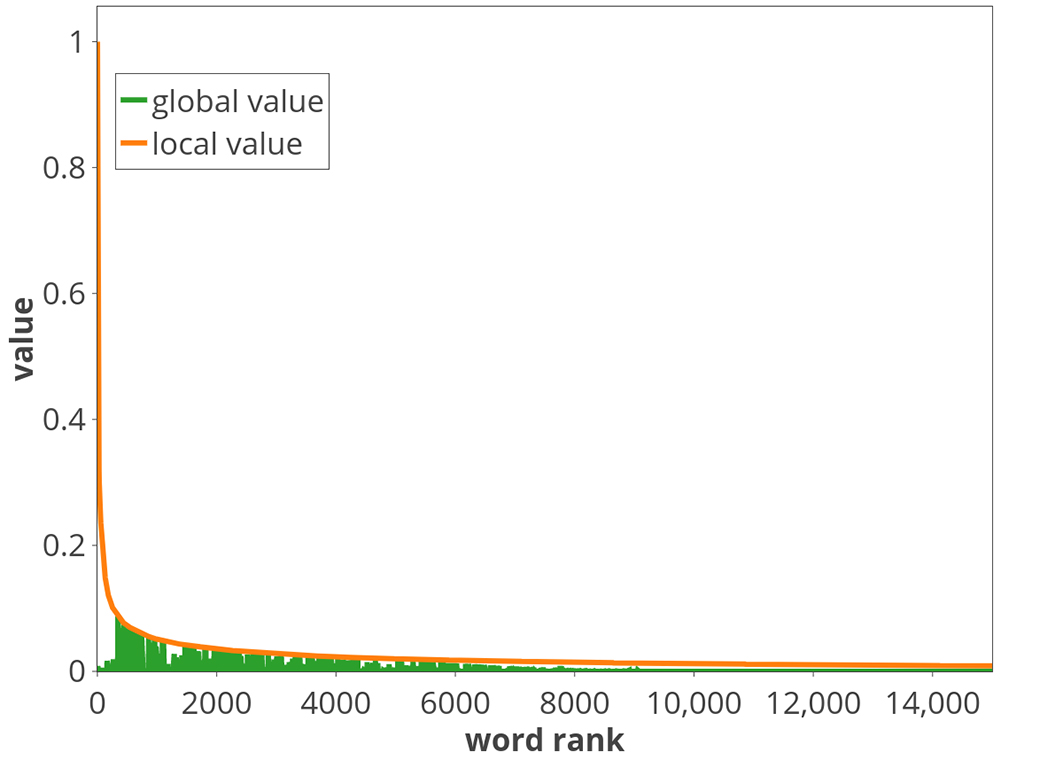
\includegraphics[width=90mm]{images/gv_negative}
%        \caption{Non-depressed}
%        \label{fig:gv_a}
%    \end{subfigure}
    % \begin{subfigure}{0.5\textwidth}
        \centering
        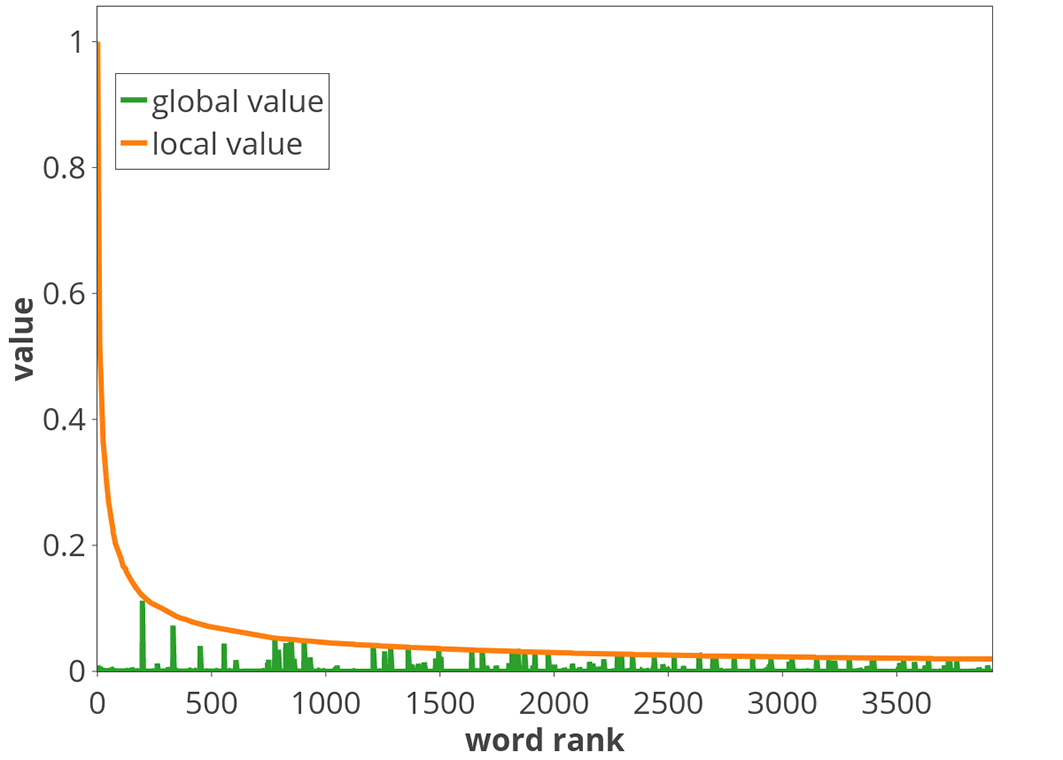
\includegraphics[width=90mm]{images/gv_positive}
        %\caption{Depressed}
        %\label{fig:gv_b}
    % \end{subfigure}
\caption{
    Curva con la distribución del \emph{valor local} de las palabras (en naranja) en contraste con la distribución del \emph{valor global} (en verde), obtenidas tras la experimentación para la clase ``depresivo''. La abscisa representa el ranking de las palabras individuales ordenadas por \emph{valor local}.
    Notar que la zona en la que se ubicarían las \emph{palabras vacías} (al comienzo de la abscisa, cercano al $0$) los \emph{valores locales} para esas palabras son los más altos (ya que el valor local de una palabra es proporcional a su frecuencia), sin embargo, como se esperaba, sus \emph{valores globales} son prácticamente $0$.
    % \emph{global value} (green) in relation to the \emph{local value} (orange) for the ``depressed'' category. The abscissa represents individual words arranged in order of frequency.
    % Note that the zone in which stop words are located (close to 0 in the abscissa) the  \emph{local value} is very high (since they are highly frequent words) but the \emph{global value} is almost 0, which is the desired behavior.
}
\label{fig:gv}
\end{figure}

\begin{figure*}[t!]
    \begin{subfigure}{0.5\textwidth}
        \centering
        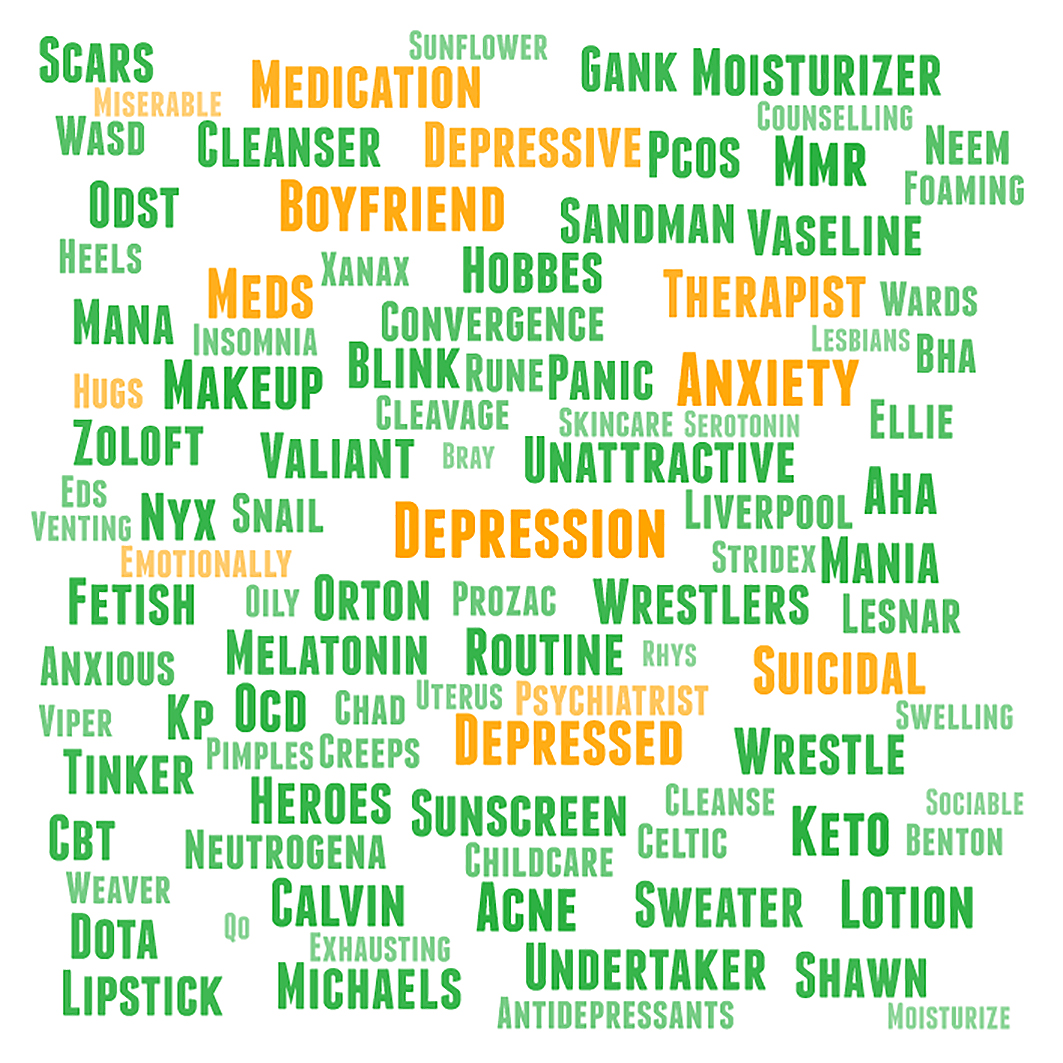
\includegraphics[width=\textwidth]{images/word-cloud-gv}
        \caption{Tamaño por \emph{valor global}}
        \label{fig:word_cloud_a}
    \end{subfigure}
    \begin{subfigure}{0.5\textwidth}
        \centering
        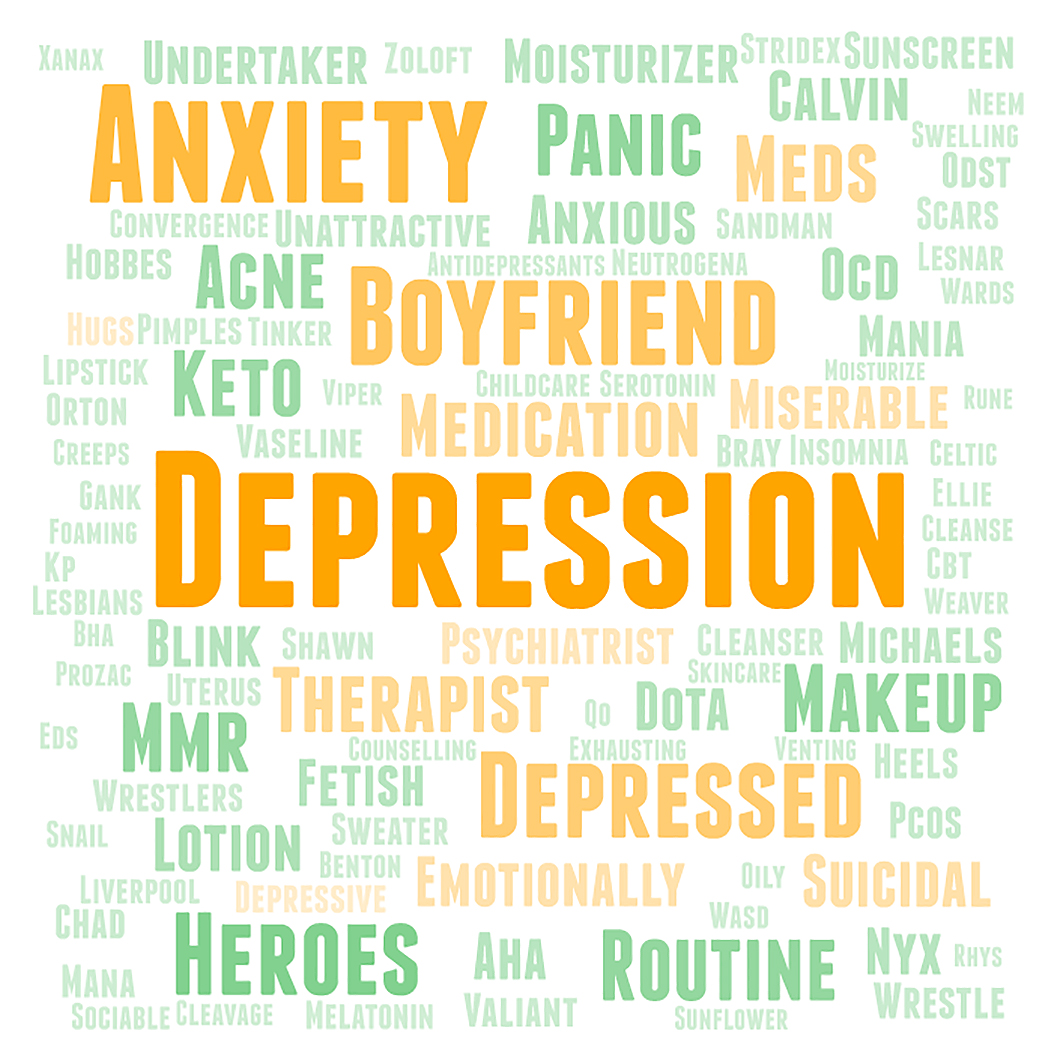
\includegraphics[width=\textwidth]{images/word-cloud-gv-fr}
        \caption{Tamaño por frecuencia en bruto}
        \label{fig:word_cloud_b}
    \end{subfigure}
\caption{
    Top 100 palabras seleccionadas por \emph{valor global} obtenidas desde el modelo, tras la experimentación.
    El tamaño de las palabras representa (a) el \emph{valor global} y (b) la frecuencia en bruto.
    Además, con fines de comparación, en naranja se marcan aquellas palabras que también fueron seleccionadas entre las 100 primeras por \emph{ganancia de información}.
    % Top-100 words selected by \emph{global value (GV)} from the model trained for the eRisk Pilot Task using chunks. The font size is related to (a) \emph{GV} and (b) row frequency. The green color indicates the words selected only by \emph{GV} whereas the orange color indicates the words also selected by the traditional Information Gain(\emph{IG}).
}
\label{fig:word_cloud}
\end{figure*}

Con el fin de intentar comprender mejor las razones que puedan estar detrás del buen desempeño del modelo en la tarea abordada, consideramos importante comenzar por analizar los valores que aprendió a asignarle a cada palabra.
En la \autoref{fig:gv} se puede corroborar que empíricamente, como esperábamos, los \emph{valores globales} en la zona en la que se deberían encontrar las palabras más importantes y discriminatorias según la ley de Zipf\footnote{Como se hipotetizó por primera vez en \cite{luhn1958automatic}, esta ley empírica sostiene que las palabras de frecuencia media en la distribución, tienen mayor importancia y poder discriminativo que las palabras con alta frecuencia.}, efectivamente, fueron los más altos. 
% In order to get a better understanding of the rationale behind the good behavior of our framework, it is important to go into more details on the mechanisms used to weight words.
% In \autoref{fig:gv} we can empirically corroborate that the \emph{global value} correctly captures the significance and discriminating power of words since, as it is well known, mid-frequency words in the distribution have both high significance and high discriminating power\footnote{As firstly hypothesized by \cite{luhn1958automatic}.}, and \emph{global values} for these mid-frequency words are the highest.
Además, la valoración aprendida de las palabras puede apreciarse desde un punto de vista más cualitativo en las nubes de palabras mostradas en la  \autoref{fig:word_cloud}. % con las 100 palabras seleccionadas por mayor \emph{valor global}.
A partir de esta figura, es posible observar que, a diferencia de la tradicional \emph{ganancia de información} que sólo consideró palabras con alta frecuencia entre sus 100 primeras (ver tamaño de palabras en naranja en (b)), el \emph{valor global} consideró además palabras que, si bien no son tan frecuentes, sí son muy discriminativas.
Para resaltar este punto, notar que el \emph{valor global} consideró palabras muy generales (como ``depression'', ``suicidal'', ``psychiatrist'', ``anxiety'', entre otras), pero, a diferencia de \emph{ganancia de información}, también incluyó muchas palabras específicas.
Por ejemplo, por medio del \emph{valor global}, SS3 no sólo aprendió a reconocer la palabra antidepresivo (``antidepressant''), sino también antidepresivos específicos como \emph{Prozac} y \emph{Zoloft}\footnote{No se incluye aquí, pero también en la posición 125 se encontraba \emph{Lexapro}.};
no sólo términos generales relacionados con medicina o trastornos (como ``medication'', ``meds'', ``insomnia'', ``panic'' o ``mania''), sino también términos más específicos como \emph{OCD} (Trastorno Obsesivo Compulsivo), \emph{PCOS} (Síndrome de Ovario Poliquístico), \emph {EDS} (Síndrome de Ehlers-Danlos), \emph{CBT} (Terapia Cognitiva Conductual), \emph{serotonina}, \emph{melatonina}, \emph{Xanax} o \emph{KP} (Kaiser Permanente, una compañía de salud);
no sólo palabras generales relacionadas con dieta, el cuerpo o la apariencia (como ``unattractive'', ``skincare'', ``makeup'' o ``acne''), sino también \emph{pimples} (granos o espinillas faciales), \emph{swelling} (hinchazón), \emph{Keto} (dieta Keto o cetogénica para la depresión), \emph{Stridex} (una medicina de tratamiento y prevención del acné), \emph{AHA} (alfa hidroxiácidos), \emph{BHA} (beta hidroxiácido), \emph{Moisturizer} (humectante), \emph{NYX} (una compañía de cosméticos) o \emph{Neutrogena} (una marca de cosméticos para el cuidado de la piel y el cabello).
Vale la pena mencionar que éste no es un aspecto menor: si valoráramos a estos términos específicos solamente por su frecuencia/probabilidad\footnote{Como es el caso, por ejemplo, al usar el clasificador \ac{MNB}.}, siempre tendrán muy poco valor, ya que, naturalmente, la probabilidad de ocurrencia de estas palabras específicas es baja en comparación con palabras más generales, como se puede observar en (b). No obstante, nosotros como humanos sabríamos intuitivamente que, por ejemplo, las oraciones ``estoy tomando antidepresivos''  y ``estoy tomando Prozac'' tienen prácticamente el mismo valor en relación a decidir si el sujeto en cuestión es depresivo o no. Afortunadamente, este aspecto es capturado correctamente por el \emph{valor global}\footnote{Notar que, a diferencia de en (b), el tamaño de ``antidepressants'' y ``prozac'', respectivamente en la parte inferior y en el centro de (a), son bastante similares y no demasiado distintas a ``depression''.}, ya que efectivamente se formuló con el fin de valorar a los términos, globalmente, en relación a qué tan discriminatorias y relevantes son para cada clase.
% 	This discriminating power of words can also be appreciated from a more qualitative point of view in the word-clouds of the top-100 selected words by \emph{global value} shown in \autoref{fig:word_cloud}.
% 	From this figure it is possible to observe that the most frequent terms, i.e. the biggest ones on (b), were also selected by $IG$ (orange colored), however, most of the terms selected only by $GV$ (green colored) are not so frequent, but highly discriminative.
% 	To highlight this point, note that \emph{GV} included very general words (depression, suicidal, psychiatrist, anxiety, etc.) but, unlike \emph{IG}, it also included many specific words.
% For instance: not only the word \emph{antidepressant} was included but also well-known antidepressants such as \emph{Prozac} and \emph{Zoloft}\footnote{Not included here, but also at rank 125 \emph{Lexapro}.};
% not only general terms related to medicine or disorders (such as \emph{medication, meds, insomnia, panic, mania}, etc.) but also more specific ones such as \emph{OCD}(Obsessive compulsive disorder), \emph{PCOS}(Polycystic ovary syndrome), \emph{EDS}(Ehlers-Danlos syndrome), \emph{CBT}(Cognitive behavioral therapy), \emph{serotonin}, \emph{melatonin}, \emph{Xanax}, \emph{KP}(Kaiser Permanente, a healthcare company), etc.;
% not only general words linked to diet, body or appearance (such as \emph{unattractive, skincare, makeup, acne}, etc.) but also \emph{pimples}, \emph{swelling}, \emph{Keto} (Ketogenic diet for depression), \emph{Stridex} (an American acne treatment and prevention medicine), \emph{AHA}(Alpha hydroxy acids), \emph{BHA}(Beta hydroxy acid), \emph{Moisturizer}, \emph{NYX} (a cosmetics company), \emph{Neutrogena} (an American brand of skin care, hair care and cosmetics), etc.
% It is also worth mentioning that this is a vital and very relevant aspect: if we value these specific words, as is usual, only by their local probability \footnote{Which is the case, for instance, with Multinomial Naive Bayes.} (or frequency), as shown in (b), they will always have almost ``no value'' since, naturally, their probability of occurrence is extremely small compared to more general words (and even worst against stopword-like terms). However, for instance, we intuitively know the phrase ``I'm taking antidepressants'' has almost the same value as ``I'm taking Prozac'' when it comes to deciding whether the subject is depressed or not.
% Fortunately, this is correctly captured by the \emph{global value}\footnote{Note that, unlike in (b), the size of ``Antidepressants'' and ``Prozac'' in (a), at the bottom and in the middle of it respectively, are quite similar and not so different from the size of ``Depression''.} since it was created to value terms, globally, according to how discriminative and relevant they are to each category.

\

\begin{figure*}[t!]
    \begin{subfigure}{0.5\textwidth}
        \centering
        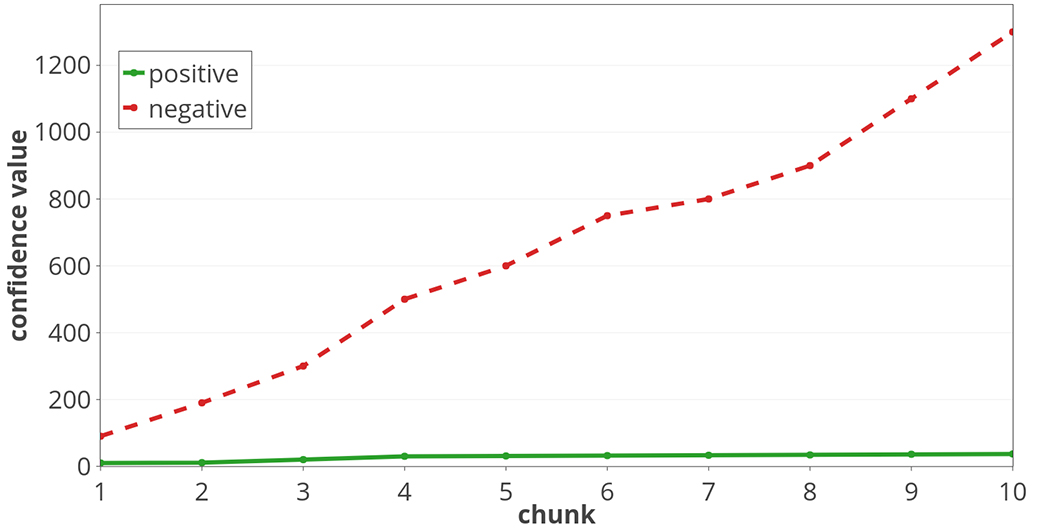
\includegraphics[width=\textwidth]{images/test_subject265}
        \caption{Sujeto 265, no depresivo.}
        \label{fig:subjects_gv_a}
    \end{subfigure}
    \begin{subfigure}{0.5\textwidth}
        \centering
        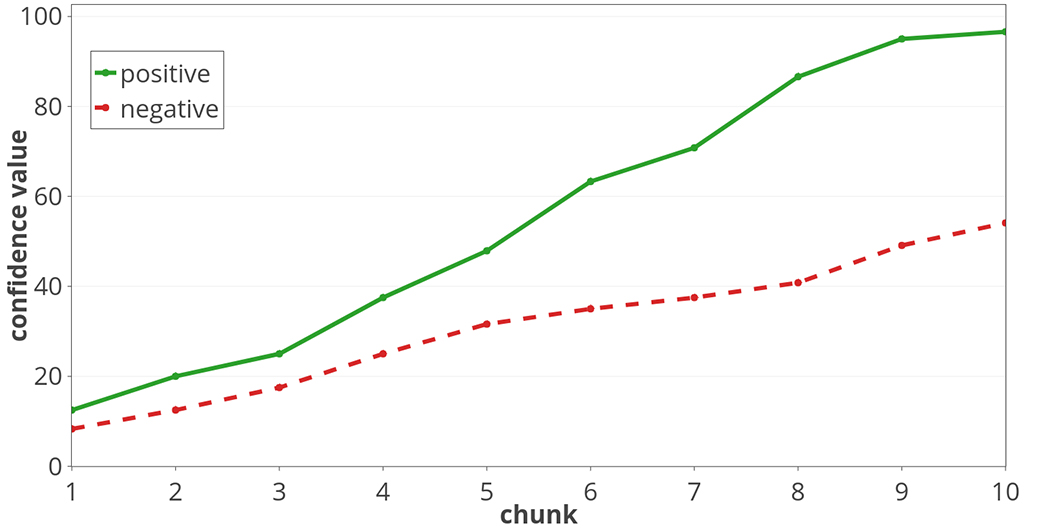
\includegraphics[width=\textwidth]{images/test_subject9306}
        \caption{Sujeto 9306, depresivo.}
        \label{fig:subjects_gv_b}
    \end{subfigure} \\
    \begin{subfigure}{0.5\textwidth}
        \centering
        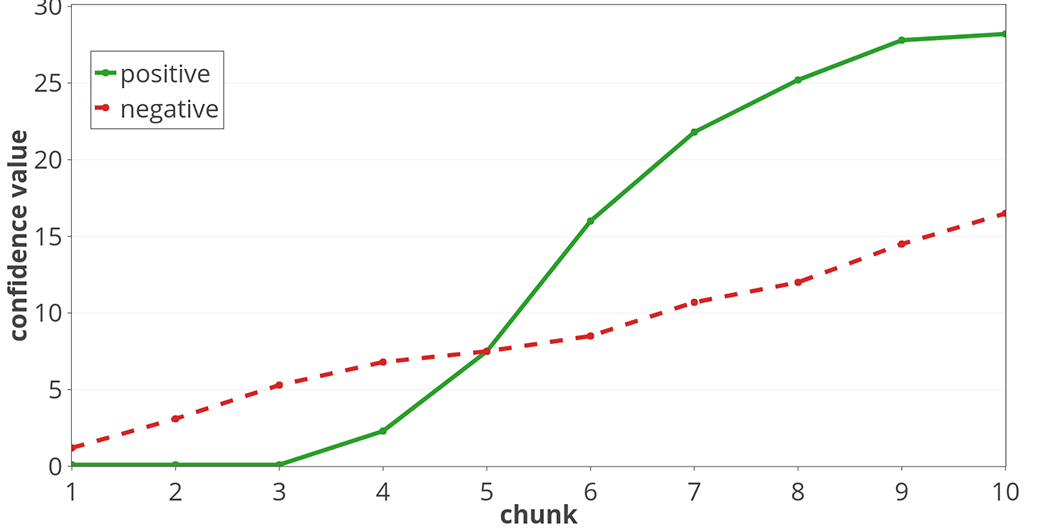
\includegraphics[width=\textwidth]{images/test_subject9579}
        \caption{Sujeto 9579, depresivo.}
        \label{fig:subjects_gv_c}
    \end{subfigure}
    \begin{subfigure}{0.5\textwidth}
        \centering
        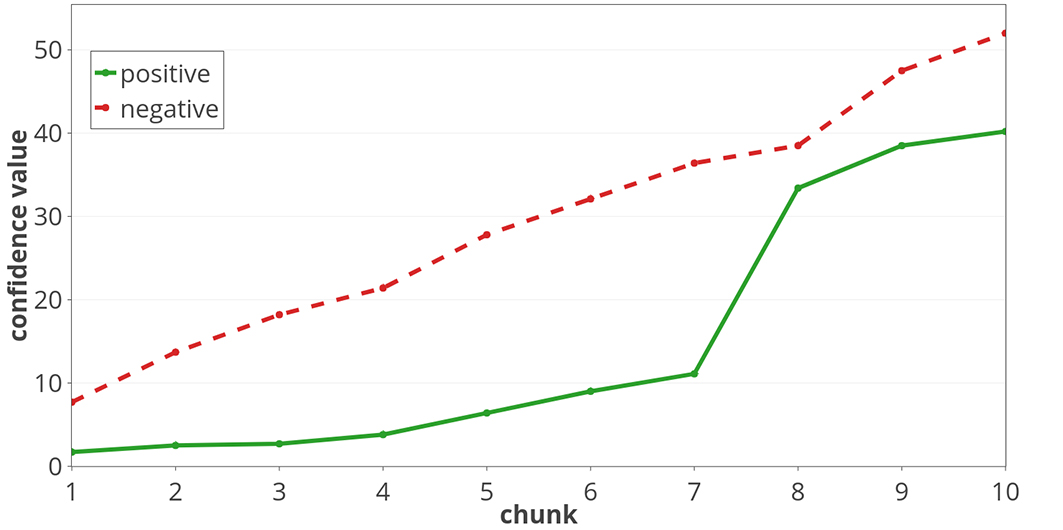
\includegraphics[width=\textwidth]{images/test_subject1914}
        \caption{Sujeto 1914, depresivo.}
        \label{fig:subjects_gv_d}
    \end{subfigure}
\caption{
\emph{Valores de confianza} acumulados a lo largo del tiempo (bloque a bloque).
Se muestran cuatro comportamientos típicos, ejemplificados cada uno con un sujeto distinto del conjunto de prueba.
% Accumulated confidence values over time (chunk by chunk).
% Four typical behaviors are shown, represented by these four subjects from the test set.
}
\label{fig:subject_cases}
\end{figure*}

Además, para comprender mejor los resultados obtenidos, otro aspecto importante a analizar es cómo  se llevó a cabo efectivamente la clasificación anticipada. 
Así, comenzaremos, primero, analizando la política más simple utilizada para decidir \emph{cuándo} clasificar positivamente a los sujetos. En la \autoref{fig:subject_cases} se muestran cuatro sujetos del conjunto de pruebas que ejemplifican cuatro tipos de comportamientos de clasificación anticipada que hemos detectado:
% Additionally, in order to better understand the good obtained results, another important aspect to analyze is how the early classification was actually carried out using the simplest policy to decide \emph{when} to positively classify subjects. In \autoref{fig:subjects_cases} are shown four subjects from the test set that illustrate four types of common classification behaviors we have detected:


\begin{itemize}
\item[(a)]
Desde el primer bloque de publicaciones en adelante, el valor de confianza de una de las clases,  ``no depresivo'' (negativo) en este caso, se mantiene siempre por encima y creciendo más rápidamente que el otro. En este ejemplo, correctamente, SS3 no pudo clasificar al sujeto como depresivo luego de haber leído todas sus publicaciones.
% from the first chunk on, the cumulative confidence value of one of the classes (negative in this case) stays above and always growing faster the other one. In this example, correctly, it was not possible to classify this subject as depressed after reading all its chunks.
\item[(b)]
Al igual que en el caso anterior, el valor de una clase (positiva en este caso) se mantiene siempre por encima de la otra, pero esta vez ambas crecen a un ritmo similar. En este ejemplo, el sujeto fue correctamente clasificado como depresivo.
% similar to the previous case, the value of one class (positive) stays always on top of the other one, but this time they both grow at a similar pace. The subject was correctly classified as depressed.
\item[(c)]
El valor de confianza negativo comienza siendo mayor que el positivo, pero a medida que se leen más publicaciones (en este caso, luego de leer el tercer bloque), el valor positivo comienza a crecer y continúa creciendo hasta superar al otro. En este ejemplo, el sujeto se clasificó correctamente como depresivo luego de que se leyera el quinto bloque de publicaciones.
% the accumulated negative confidence value starts being greater than the positive one, but as more chunks are read (specifically starting after reading the 3rd chunk), the positive value starts and stays growing until it exceeds the other one. In this case, this subject is classified as depressed after reading the 6th chunk.
\item[(d)]
Este ejemplo muestra un comportamiento similar al anterior. Sin embargo, si bien el valor positivo se acerca mucho al negativo, nunca alcanza a superarlo. Esto provocó que  el sujeto no haya podido ser clasificado correctamente como depresivo.
% this example has a behavior similar to the previous one, however, the positive value, despite getting very close at chunk 8, never exceeds the negative one, which leads to the subject 1914 being misclassified as negative.
\end{itemize}

\begin{figure}[t!] % [t]op; [h]ere; [p]age; [b]ottom; [r]ight; [l]eft
    \centering
    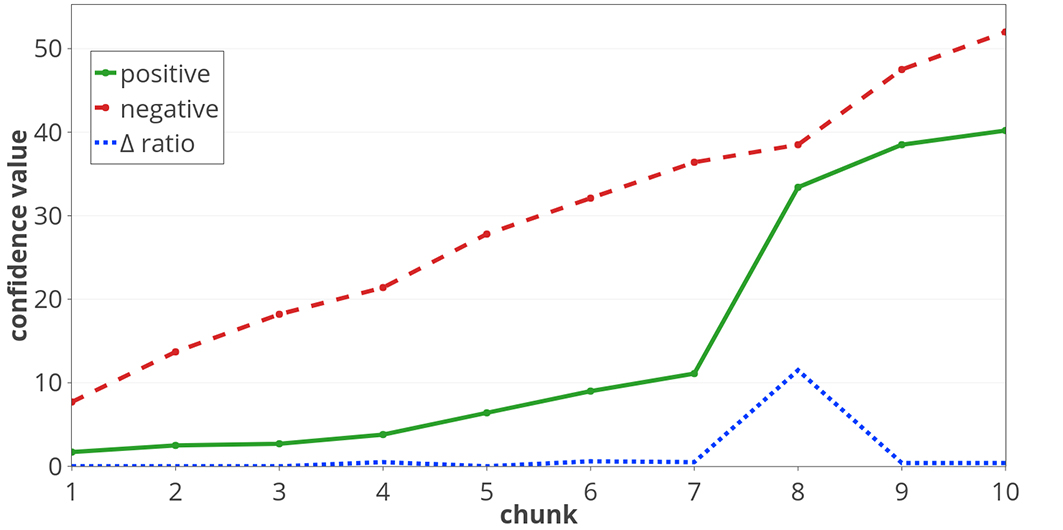
\includegraphics[width=120mm]{images/test_subject1914_slope}
    \caption{
    Sujeto 1914, depresivo.
    La tasa de cambio ($\Delta$) entre la curva positiva y negativa se muestra en azul (línea de puntos). Este cambio $\Delta$ fue el utilizado en la política del modelo $SS3^\Delta$.
    Notar que la línea azul tiene un pico en el bloque 8, lo que en este caso indica que el valor positivo ha crecido alrededor de 11 veces más rápido que el negativo, en ese punto.}
    % The ratio between the positive and the negative slope change ($\Delta$) is shown in blue dotted line. This ratio was used by the $\Delta$ policy.}
\label{fig:slope}
\end{figure}

La razón por la que se decidió implementar un segundo modelo, $SS3^\Delta$, fue para intentar evitar errores de clasificación similares al ejemplificado en (d). Es por esto que se decidió que su política también tenga en cuenta el crecimiento del \emph{valor de confianza} positivo en relación al negativo.
Más precisamente, como se puede ver en el \autoref{alg:classification_ss3slope}, y como se mencionó anteriormente, $SS3^\Delta$ clasifica un sujeto no sólo cuando el valor positivo supera al negativo, sino también cuando el valor positivo crece, al menos, cuatro veces más rápido que el negativo.
En la \autoref{fig:slope} se muestra nuevamente al sujeto 1914 (\autoref{fig:subjects_error_d}), pero esta vez se incluye información sobre los cambios en la pendiente de los valores.
Notar que este sujeto fue clasificado previamente como no depresivo porque el valor positivo nunca superó al negativo, pero utilizando esta nueva política, luego de leer el octavo bloque sí pudo ser clasificado correctamente.
% With the aim of avoiding cases of misclassification like in (d), we decided to implement the second classifier, SS3$^\Delta$, whose policy also takes into account the changes in both slopes.
% As it can be seen from \autoref{alg:classification_ss3slope} and as mentioned before, SS3$^\Delta$ additionally classifies a subject as positive if the positive slope changes, at least, four times faster than the other one.
% In \autoref{fig:slope} is shown again the subject 1914, this time including information about the changes in the slopes.
% Note that this subject was previously misclassified as not depressed because the accumulated positive value never exceeded the negative one, but by adding this new extra policy, this time it is correctly classified as positive after reading the 8th chunk\footnote{Note the peek in the blue dotted line pointing out that, at this point, the positive value has grown around 11 times faster than the negative one.}.

\begin{algorithm}[t!]
\small
\caption{\small
Algoritmo de clasificación anticipada utilizado por SS3$^\Delta$.
Donde \textproc{Clasificar-Bloque}($bloque$) es en realidad un alias de  \textproc{Clasificar-A-Nivel}($bloque$, 4) (dado en \autoref{alg:classification}).
}
  \label{alg:classification_ss3slope}
  \begin{algorithmic}[h]
  \Statex
  \Function{Clasificar-Sujeto}{$bloques$}
      \State \Input $bloques$, secuencia de bloques (de publicaciones)
      \State \LocalVariables $\overrightarrow{c}$, el \emph{vector de confianza} del sujeto
      \State \localvarsindent $\overrightarrow{\Delta c}$, el \emph{vector de confianza} de un bloque
      %\State
      \State $\overrightarrow{c} \gets \langle 0, 0\rangle$ $\rhd$ de la forma $\langle negativo, positivo\rangle$
      \For{$bloque$ \textbf{en} $bloques$}
          \State $\overrightarrow{\Delta c} \gets $\Call{Clasificar-Bloque}{$bloque$}
          \State $\overrightarrow{c} \gets \overrightarrow{c} + \overrightarrow{\Delta c}$ 
          %\State
          \If {$\frac{\overrightarrow{\Delta c}[1]}{\overrightarrow{\Delta c}[0]} > 4$ \Or $\overrightarrow{c}[1] > \overrightarrow{c}[0]$}
              \State \Return $positivo$ \Comment{clasificarlo como depresivo}
          \Else
              \State se requiere más evidencia
          \EndIf
      \EndFor
      %\State
      \State \Return $negativo$ \Comment{clasificarlo como no depresivo}
  \EndFunction
  \end{algorithmic}
\end{algorithm}

Como lo sugiere este último análisis, está claro que se puede obtener información útil del estudio de aquellos casos en los que el modelo no pudo clasificar correctamente a los sujetos. Con este objetivo en mente, también decidimos llevar a cabo un análisis de error, identificando así cuatro tipos de errores comunes, que podrían dividirse en dos grupos: los que, creemos, surgieron de un etiquetado incorrecto del conjunto de prueba y los que surgieron de un mal desempeño del clasificador en sí. En la \autoref{fig:subjects_error} se caracteriza cada tipo de error, nuevamente, utilizando cuatro sujetos del conjunto de prueba:
% From the previous analysis, it is clear that useful information can be obtained from the study of those cases where our approach was not able to correctly predict a class. With this goal in mind, we also carried out an error analysis and identified four common error cases which could be divided into two groups: those that arise from a bad labeling of the test set and those that arise from bad classifier performance. In \autoref{fig:subjects_error} we exemplify each case with one subject from the test set, described in more detail below:

\begin{figure*}[t!]
    \begin{subfigure}{0.5\textwidth}
        \centering
        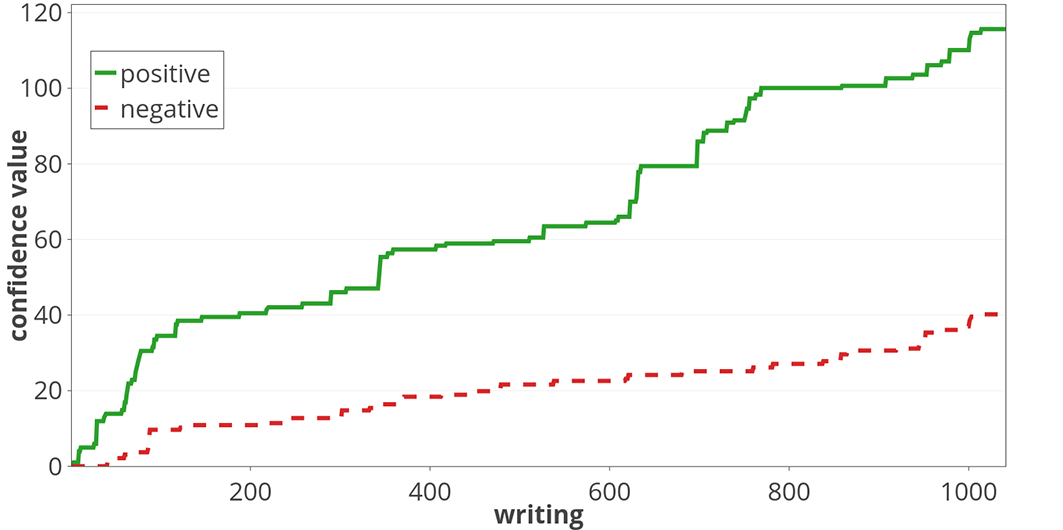
\includegraphics[width=\textwidth]{images/error1_test_subject834}
        \caption{Sujeto 834, no depresivo.}
        \label{fig:subjects_error_a}
    \end{subfigure}
    \begin{subfigure}{0.5\textwidth}
        \centering
        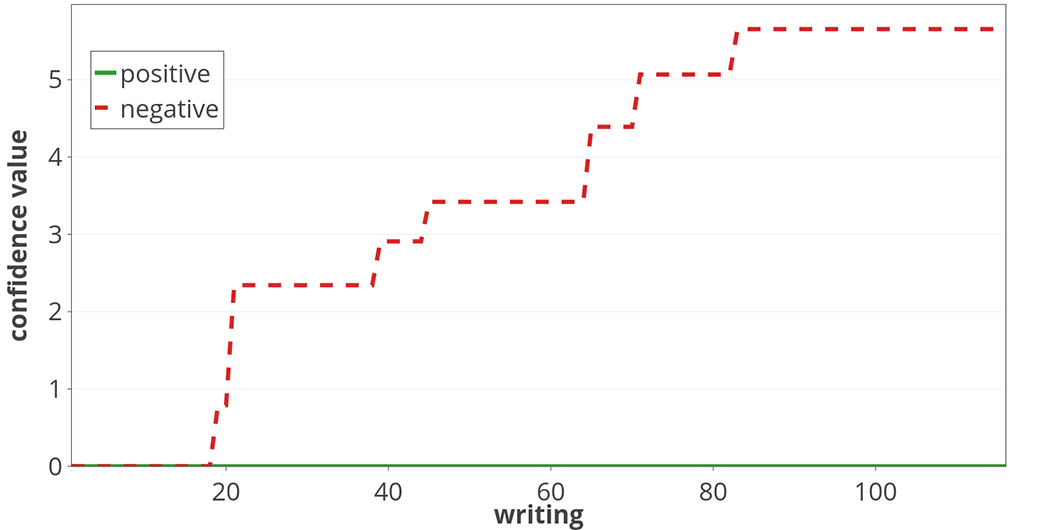
\includegraphics[width=\textwidth]{images/error2_test_subject1345}
        \caption{Sujeto 1345, depresivo.}
        \label{fig:subjects_error_b}
    \end{subfigure} \\
    \begin{subfigure}{0.5\textwidth}
        \centering
        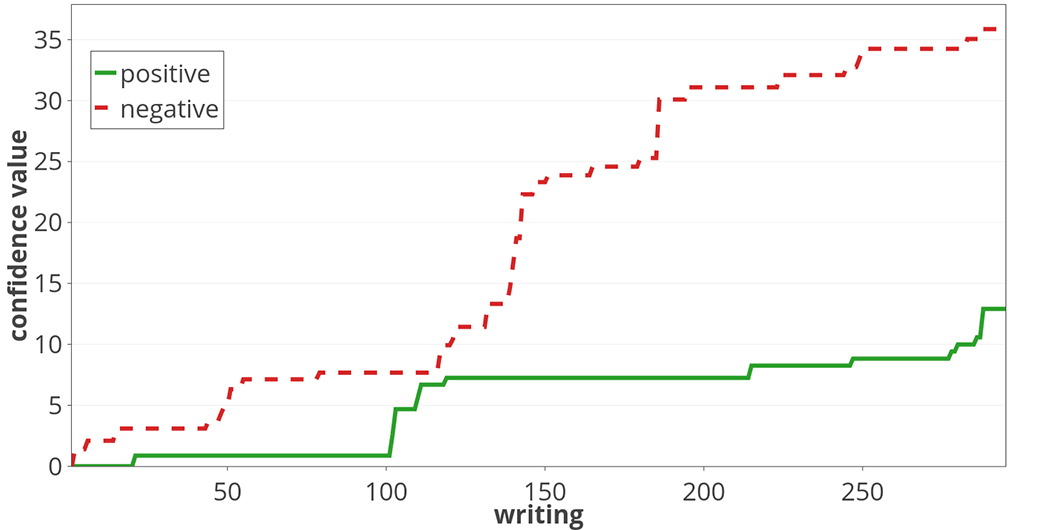
\includegraphics[width=\textwidth]{images/error3_test_subject2673}
        \caption{Sujeto 2673, depresivo.}
        \label{fig:subjects_error_c}
    \end{subfigure}
    \begin{subfigure}{0.5\textwidth}
        \centering
        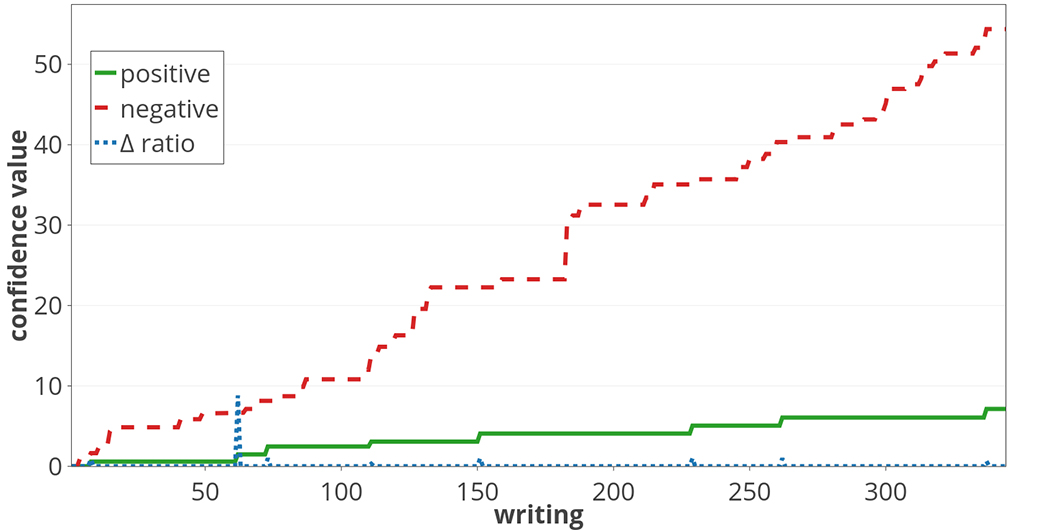
\includegraphics[width=\textwidth]{images/error4_test_subject748}
        \caption{Sujeto 748, no depresivo.}
        \label{fig:subjects_error_d}
    \end{subfigure}
\caption{
\emph{Valores de confianza} acumulados a lo largo del tiempo (publicación a publicación).
Se muestran cuatro casos comunes de error, cada uno ejemplificado con un sujeto del conjunto de prueba.
% Accumulated confidence values over time (writing by writing).
% Four common error cases, represented by these four subjects.
}
\label{fig:subjects_error}
\end{figure*}

\begin{itemize}
\item[(a)]
El sujeto se clasifica erróneamente como positivo ya que, efectivamente, el valor positivo superó y continuó superando al negativo. Tras un análisis manual de casos similares a éste, a menudo descubrimos que, al parecer, el clasificador no estaba equivocado al ``acumular confianza'' positiva, ya que a nuestro parecer, dichos sujetos eran efectivamente depresivos.\footnote{Por ejemplo, encontramos oraciones tales como la siguiente: ``Comencé la TCC (Terapia de conducta cognitiva) pero nunca la terminé. Es realmente difícil hacer TCC para depresión y ansiedad cuando además soy psicótico, gracias por darme apoyo moral, por así decirlo''.}
% the subject is misclassified as positive since the positive accumulated exceeded the negative one. When we manually analyzed cases like these we often found out that the classifier was correctly accumulating positive evidence since the users were, in fact, depressed.
% \footnote{We found sentences like this one: ``I did start CBT but I never finished it. It's really hard to do CBT for depression and anxiety when I'm psychotic, thank you for giving moral support so to speak''}.
\item[(b)]
En casos como éste, los sujetos se clasificaron erróneamente como negativos, debido a que SS3 no acumuló ninguna (o muy poca) evidencia positiva. Analizando manualmente las publicaciones de los sujetos, tampoco pudimos encontrar evidencia de que efectivamente fueran depresivos.\footnote{Los sujetos sólo hablaban sobre ciertos temas en general, tales como deportes, música, etc.}
% in cases like this one, subjects were misclassified as negative, since SS3 did not accumulate any (or very little) positive evidence. Manually analyzing the writings, we often could not find any positive evidence either, since subjects were talking about topics not related to depression (sports, music, etc.).
\item[(c)]
Hubo casos como el presentado aquí, en los que SS3 no pudo clasificar al sujeto como  depresivo,  debido a que el valor positivo acumulado no pudo superar el negativo, aun cuando en ocasiones pudo acercarse mucho. Notar que, cerca de la publicación número 100, el valor positivo se acerca mucho al negativo pero no alcanza a superarlo.\footnote{Quizás un ajuste más fino de los hiperparámetros podría superar este problema.}
% there were cases like this subject, in which SS3 failed to predict ``depression'' due to the accumulated positive value not being able to exceed the negative one even although, in some cases, it was able to get very close. Note that the positive value gets really close to the negative one at around the 100th writing.
% \footnote{Perhaps a finer tuning of hyper-parameters would overcome this problem.}
\item[(d)]
Este tipo de error se introdujo con la utilización de la política de $SS3^\Delta$.
En algunos casos, SS3 clasificó erróneamente a los sujetos como depresivos porque, si bien era cierto que el valor positivo cambió al menos 4 veces más rápido que el negativo, esta condición era verdadera debido a que el cambio negativo había sido muy pequeño (y no porque el positivo haya sido muy grande).
Por ejemplo, si el aumento del valor negativo fuese de $0.01$, un aumento positivo realmente pequeño, de al menos $0.04$, sería suficiente para disparar la decisión de ``clasificar como positivo''.\footnote{Quizás esto podría solucionarse al agregar una condición extra para controlar que el aumento positivo o negativo sea, al menos, mayor que alguna constante fija.}
En este ejemplo, este problema puede observarse en el pico azul punteado alrededor de la publicación 60, indicando que ``el valor positivo cambió cerca de 10 veces más rápido que el negativo''. En ese punto se clasifica erróneamente al sujeto como depresivo ya que el aumento de valor positivo fue, de hecho, muy pequeño.
% this type of error occurred only due to the addition of the slope ratio policy.
% In some cases, SS3 misclassified subjects as positive because, while it was true that the positive value changed at least 4 times more rapidly than the negative, the condition was mainly true only due to the negative change being very small.
% For instance, if the change of the negative confidence value was 0.01, a really small positive change of at least 0.04 would be enough to trigger the ``classify as positive'' decision.
% \footnote{Perhaps this could be fixed if we also request the positive or negative change to be, at least, bigger than a fixed constant (let us say 1) before applying the policy.}
% This problem can be detected in this subject by seeing the blue dotted peek at around the 60th writing, indicating that ``the positive slope changed around five times faster than the negative'' there, and therefore misclassifying it as positive. However, note that this positive change was in fact really small (less than 1). 
\end{itemize}


\begin{figure}[t!]
	\small
    \begin{subfigure}{\textwidth}
    	\centering
        \fbox{
        \begin{minipage}{0.9\textwidth}
        	\textbf{$\cdots$}\newline
        	\hlinew
            \textbf{Publicación 54 $\blacktriangleright$} I'm going to agree with everyone else and say you definitely need a lawyer. Get in touch with the[...]\newline
			\hlinew
			\textbf{Publicación 55 $\blacktriangleright$} \sethlcolor{dgreen_25}\hl{You don't mention what the fertility issue is (and you don't have to) but his feelings may stem fr[...]}\newline
            \hlinew
%            \textbf{Publicación 56 $\blacktriangleright$} Limited Experience . I am going through a divorce (yay, fun times) and while I don't think I'll [...]\newline
%            \hlinew
            \textbf{$\cdots$}\newline
            \hlinew
            \textbf{Publicación 59 $\blacktriangleright$} Thankfully I was able to realize that I was in a bad place and get help. My sister has been awesom[...]\newline
            \hlinew
            \textbf{Publicación 60 $\blacktriangleright$} \sethlcolor{dgreen_90}\hl{I have been seeing a therapist which I think is helping a little. Fact is, I was feeling really depressed[...]}\newline
            \hlinew
            \textbf{Publicación 61 $\blacktriangleright$} \sethlcolor{dgreen_50}\hl{My Wife Wants a Divorce . This will be long, sorry in advance. My wife told me shortly after the[...]}\newline
			\hlinew
            \textbf{Publicación 62 $\blacktriangleright$} the Earth Arena coming up I have: Zelnite x2 Dilma Ophelia For my last spot, should I use Miku[...]\newline
			\hlinew
            \textbf{$\cdots$}
        \end{minipage}
        }
        \caption{Historial del sujeto 9579 - nivel publicación\vspace{4mm}}
        \label{fig:subject9579_descriptive_a}
    \end{subfigure} \\
    \begin{subfigure}{0.5\textwidth}
        \centering
        \fbox{
        \begin{minipage}{0.9\textwidth}
			\sethlcolor{dgreen_25}\hl{I have been seeing a therapist which I think is helping a little}. \sethlcolor{dgreen_90}\hl{Fact is, I was feeling really depressed and wanting to kill myself}. I spent basically all of Feb in the hospital[...]
       	\end{minipage}
        }
        \caption{Publicación 60 - nivel oración}
        \label{fig:subject9579_descriptive_b}
    \end{subfigure}
    \begin{subfigure}{0.5\textwidth}
        \centering
        \fbox{
        \begin{minipage}{0.9\textwidth}
			I have been seeing a \sethlcolor{dgreen_50}\hl{therapist} which I think is helping a little. Fact is, I was \sethlcolor{dgreen_25}\hl{feeling} really \sethlcolor{dgreen_70}\hl{depressed} and wanting to kill \sethlcolor{dgreen_25}\hl{myself}. I spent basically all of Feb in the hospital[...]
       	\end{minipage}
        }
        \caption{Publicación 60 - nivel palabra}
        \label{fig:subject9579_descriptive_c}
    \end{subfigure}
    \caption{Esta figura muestra cómo se podría brindar una explicación visual del proceso de clasificación en la tarea abordada. Como mencionamos anteriormente, SS3 nos permite visualizar las razones detrás de la clasificación en diferentes niveles, en nuestro caso: (a) publicaciones, párrafos, (b) oraciones y/o (c) palabras. Cada uno de los segmentos está coloreado en relación al \emph{valor de confianza} positivo, real, obtenido en los experimentos realizados.}
% \caption{This figure shows how a visual description of the decision process could be given in this depression detection task. As we mentioned before, our framework allows us to analyze the reasons behind its classification decision, at different levels: (a) writings, (b) sentences and (c) words, etc. Each one of these blocks is painted proportionally to the real positive \emph{confidence values} we obtained after the experiments.}
\label{fig:subject9579_descriptive}
\end{figure}


Finalmente, creemos que es apropiado volver a examinar otra de las virtudes del modelo: \emph{su transparencia}.
Como se examinó anteriormente en la \autoref{sec:EC} del \autoref{cap3}, la mayoría de los clasificadores actúan como cajas negras, tanto tradicionales como modelos avanzados de \emph{aprendizaje profundo}.
% Esto es, el proceso de clasificación no se explica naturalmente por sí mismo y, por lo tanto, los humanos difícilmente pueden interpretar las razones detrás de la clasificación.
Sin embargo, como vimos y al igual que con cualquier otra tarea sensible o de detección de riesgo, con el fin de brindar ciertas garantías de confiabilidad, idealmente se espera que los modelos sean capaces de explicar o mostrar, de algún modo, las razones que lo llevaron a clasificar a los usuarios como tal.
% Sin embargo, como vimos, este es un aspecto esencial cuando la tarea involucra decisiones sensibles o de riesgo en las que, por lo general, personas reales están involucradas.
Así, en la  \autoref{fig:subject9579_descriptive} se muestra un ejemplo de lo que podría ser una explicación visual, dada por SS3, del proceso de clasificación para el sujeto 9579.\footnote{Notar que éste es el mismo sujeto que se utilizó anteriormente en el ejemplo mostrado al comienzo de este capítulo, en la \autoref{fig:subject9579_writings} de la \autoref{sec:classification_process}. Los lectores interesados pueden encontrar la relación entre la curva verde (positiva) mostrada allí y la intensidad del color de cada publicación mostrada en la \autoref{fig:subject9579_descriptive_a}.}
En este ejemplo se muestra en (a) un segmento del historial de publicaciones del sujeto, el cual ha sido coloreado en relación al \emph{valor de confianza} positivo asignado por SS3 ---lo que nos indica cuáles fueron las publicaciones involucradas, y en qué medida, en la decisión de clasificar al sujeto como positivo. Además, si un especialista quisiera analizar a su vez, digamos, la publicación 60 con más detalle, el mismo proceso podría utilizarse para los distintos niveles de la jerarquía que SS3 construye para clasificar, como por ejemplo se muestra en (b) y (c) para los niveles de oraciones y de palabras, respectivamente.
Vale la pena mencionar que debido a que este proceso de visualización se puede automatizar de una forma directa, utilizando los valores de los distintos \emph{vectores de confianza} de la jerarquía, hemos desarrollado una demo en línea, especialmente creada para este propósito, disponible en \url{http://tworld.io/ss3} ---por medio de esta demo los usuarios pueden probar ``en vivo y en directo'' a SS3 que, junto con el resultado de clasificación en sí mismo, brinda una explicación visual e interactiva de la clasificación.\footnote{De momento se encuentran disponibles dos modelos a probar, uno entrenado para el análisis de sentimientos en reseñas de películas y otro para clasificación temática.}
% Finally, we believe it is appropriate to highlight another of the highly desirable aspects of our Framework: its descriptive capacity.
% As mentioned previously in \autoref{sec:requeriments}, most of the classical and state-of-the-art classifiers act as black boxes (i.e. classification process is not self-explainable) and therefore humans are not able to naturally interpret the reasons behind the classification.
% However, this is a vital aspect, especially when the task involves sensitive or risky decisions in which, usually, people are involved. In \autoref{fig:subject9579_descriptive} is shown an example of a piece of what could be a visual description of the classification process for the subject 9579.
% \footnote{Note that this is the same subject who was previously used in the example shown in \autoref{fig:subject9579_writings}, in \autoref{sec:classification_process}. The interested readers could see the relation between the green/positive curve there and the color intensity of each writing shown in \autoref{fig:subject9579_descriptive_a}.}
% In this example, we show in (a) a painted piece of the subject's writings history that the system users could use to identify which were the writings involved, and to what degree, in the decision making (classification) process. if the user wanted to further analyze, let us say, the writing 60 in more details, the same process could be applied at two different lower levels, as shown in (b) and (c) for sentences and words respectively.
% It is worth mentioning that since this ``descriptive process'' can be easily automated we have developed an online live demo, especially built for this purpose, available at \href{http://tworld.io/ss3}{http://tworld.io/ss3}, in which users can try out a version of SS3 trained using tweets for topic classification (music, sports, etc.) that, along with the classification result, gives a visual description.


\subsection{Implicaciones y Consideraciones Clínicas}
% \subsection{Implications and Clinical Considerations}
\label{sec:implications_clinical}

Antes de finalizar este capítulo, dada la naturaleza del problema abordado, creemos importante examinar las implicaciones y consideraciones clínicas del trabajo realizado.

Como se resalta en Guntuku \emph{et al.} \cite{guntuku2017detecting}: ``Los métodos de detección automática pueden ayudar a identificar a personas depresivas o en riesgo a través del monitoreo pasivo, a gran escala, de las redes sociales, y en el futuro pueden complementar los procedimientos de detección existentes''.
En ese contexto, el modelo propuesto podría servir como un marco de trabajo con el que se podrían desarrollar sistemas, en un futuro, para el monitoreo pasivo a gran escala de las redes sociales que permita ayudar a detectar los primeros rastros de depresión analizando los patrones lingüísticos de los usuarios. Por ejemplo, dicho sistema podría filtrar usuarios presentando posibles candidatos, junto con información visual e interactiva, a profesionales de la salud mental para ser analizados manualmente. El aspecto de ``monitoreo pasivo a gran escala'' estaría respaldado, en principio, por la naturaleza paralelizable e incremental de SS3,\footnote{Sólo se requeriría almacenar un pequeño vector bidimensional, el \emph{vector de confianza}, por cada usuario.} mientras que la presentación de ``información visual e interactiva'' a los profesionales, por su naturaleza de caja blanca y la capacidad de explicar visualmente la clasificación.
Está claro que el trabajo abordado en esta tesis doctoral \emph{no persigue un objetivo de diagnóstico automático}, sino más bien el de brindar las bases para desarrollar, a futuro, herramientas de monitoreo complementarias a otros métodos bien establecidos dentro del estudio de la salud mental.
De hecho, varios problemas éticos y legales sobre la privacidad y protección de datos, y sobre cómo integrar efectivamente este tipo de métodos dentro de sistemas de salud, siguen siendo problemas abiertos de investigación~\cite{guntuku2017detecting}.
% As stated in \cite{guntuku2017detecting}: ``Automatic detection methods may help to identify depressed or otherwise at-risk individual through the large-scale passive monitoring of social media, and in the future may complement existing screening procedures''.
% In that context, our proposal is a potential tool with which systems could be developed in the future for large-scale passive monitoring of social media to help detecting early traces of depression by analyzing users' linguistic patterns, for instance, filtering users and presenting possible candidates, along with rich and interactive visual information, for mental health professionals to manually analyze them. The ``large-scale passive monitoring'' aspect would be supported by the incremental\footnote{Only one small vector, the \emph{confidence vector}, needs to be stored for each user.} and highly parallelized nature of SS3 while the ``rich and interactive visual information'' one by its white-box nature.
%is able to early detect certain linguistic patterns in the use of language of individual diagnosed with depression.
% It is clear that this work \emph{does not pursue a goal of autonomous diagnosis} but rather being a complementary tool to other well-established methods of mental health.
% As a matter of fact, several ethical and legal questions about data ownership and protection, and how to effectively integrate this type of approaches into systems of care are still open research problems \cite{guntuku2017detecting}.

El conjunto de datos utilizado en este trabajo tiene la ventaja de estar abierto al público y, si bien desempeñó un papel importante al impulsar el estudio de la relación entre el uso del lenguaje y el problema de detección de depresión, éste presenta algunas limitaciones desde un punto de vista metodológico/clínico.
Más allá del posible ``ruido'' introducido por el método utilizado para construir los grupos de usuarios  ``depresivos'' y ``no depresivos'', el conjunto de datos carece de cierta información adicional que podría ser muy valiosa para el problema de detección de depresión.
Por ejemplo, en otros conjuntos de datos, como el utilizado en De Choudhury \emph{et al.} \cite{de2013social}, además del texto propiamente dicho (tweets), también incluyen información muy valiosa y específica para este tipo de patología, como son los puntajes obtenidos en diferentes tests de depresión (\emph{CES-D} y \emph{BDI}), información sobre la red de contactos del usuario, índice de insomnio y patrones de publicación, entre otros.
Está claro que si hubiéramos tenido acceso a este tipo de información adicional, habría sido posible obtener, entre otros, una evaluación más confiable de los sujetos depresivos, el grado de severidad de la depresión, así como también la detección de algunos factores mediadores, como cambios de humor u ambientales, que podrían no ser directamente inferidos de las publicaciones de los usuarios.
Además, esta información también podría usarse para entrenar otros modelos e integrar sus predicciones con las obtenidas usando solamente información textual, por ejemplo, por medio del uso de métodos de ensamble de clasificadores.
% The dataset used in this task had the advantage of being publicly available and played an important role in determining how the use of language is related to the EDD problem. However, it exhibits some limitations from a methodological/clinical point of view. Beyond the potential ``noise'' introduced by the method to assess the ``depressed''/``non-depressed'' condition, it lacks some extra information that could be very valuable to the EDD problem.
% For instance, in other datasets, such as the one used in \cite{de2013social} for the detection of depression in social media (Twitter in this case), in addition to the text of the interactions (tweets), it was also available other extremely valuable information for this type of pathology such as the scores obtained in different depression tests (CES-D and BDI), information about the user's network of contacts and interaction behavior (such as an insomnia index and posting patterns), among others.
% It is clear that if we had had this additional information available, it would have been possible to obtain, among others, a more reliable assessment of depressive people, their severity levels of depression, and also to detect some mediating factors like environmental changes that could not be directly available in the users’ posts.
% Besides, this information could also be used to train other models and integrate their predictions with the ones obtained only using textual information by, for instance, using some late-fusion ensemble approach.

Finalmente, aunque la interpretación clínica de los resultados no se abordó en nuestro trabajo, es importante resaltar algunos puntos importantes.
En primer lugar, fue interesante observar que la mayoría de las 100 palabras identificadas por SS3, seleccionadas por mayor \emph{valor global}, se corresponden perfectamente a las categorías habitualmente identificadas en otros estudios más clínicos sobre depresión ---tales como palabras relacionadas a síntomas, tratamientos, divulgación/revelación (disclosure), relaciones/vida (relationships-life) \cite{ de2013social}.
Curiosamente, también notamos lo que podría llegar a ser una potencial nueva clase de palabras, aquellas vinculadas a los videojuegos multijugador en línea,\footnote{Como se puede ver en \autoref{fig:word_cloud}, por ejemplo, por las palabras vinculadas al popular videojuego Dota, como son ``Dota'', ``MMR'', ``Wards'', ``Mana'', ``Rune'', ``Gank'', ``Heroes'' y ``Viper''.}   sin embargo, un análisis serio de esto requeriría de un trabajo multidisciplinario con profesionales de la salud mental, lo que está fuera del alcance del presente trabajo.
Por otro lado, los gráficos que presentan los \emph{valores de confianza} acumulados a lo largo del tiempo, como son los de la \autoref{fig:subjects_error}, tienen la intención de mostrar cómo la evidencia léxica (aprendida desde los datos de entrenamiento y dada por la función $gv$) se acumula y varía con el tiempo ---y cómo ésta es usada por el modelo para decidir \emph{cuándo} se dispone de suficiente evidencia como para clasificarla.
Estos gráficos no deben interpretarse erróneamente como un intento de capturar cambios de humor u otros comportamientos típicos en personas depresivas.
Tenga en cuenta que, como se mencionó anteriormente, este tipo de información sí podría integrarse en nuestro modelo a través de métodos de ensamble de clasificadores, sin embargo, dado que no disponemos de un conjunto de datos que brinde este tipo de información, su implementación está más allá del alcance de este trabajo y será considerada como trabajo a futuro.
De hecho, creemos que la ampliación del modelo predictivo mediante la incorporación de este tipo de información vinculada a aspectos no lineales del comportamiento humano, como los cambios de humor, podría ayudar a capturar la variación de los síntomas de depresión a lo largo del tiempo.
Esto, por ejemplo, podría ayudar a detectar cuando los síntomas empeoran, como un medio para prevenir un posible suicidio o, si el sujeto ya está diagnosticado, para detectar cuando la terapia aplicada no está funcionando adecuadamente.
% Tener acceso a un conjunto de datos con este tipo de información de comportamiento permitiría, en el futuro, integrarlo al modelo mediante, por ejemplo, enfoques de ensamble de modelos.
% We believe that extending the predictive model by incorporating information related to non-linear aspects of human behavior, such as mood shifts, could help to capture when depression symptoms ``wax and wane''. This, for example, could help to detect when symptoms worsen as a means to prevent possible suicide or, if the subject is already diagnosed, to detect when applied therapy is not working. Having access to a dataset with this type of behavioral information would allow us in the future to integrate it into our EDD framework through, for example, a late-fusion ensemble approach.
\hfill$\square$



%\acresetall
%\chapter{Un Clasificador con n-gramas Dinámicos para la Detección Anticipada de Riesgos en Redes Sociales}
% \chapter{Un clasificador con n-gramas dinámicos para la detección anticipada de riesgos: Depresión y anorexia en redes sociales}
%\label{cap:tss3}
%\emph{Como producto del trabajo presentado en este capítulo surgió el artículo publicado en ``Pattern Recognition Letters'', volume 138, titulado ``$\tau$-SS3: A text classifier with dynamic n-grams for early risk detection over text streams''.}\footnote{\url{https://doi.org/10.1016/j.patrec.2020.07.001}}

\

El presente capítulo tiene como principal objetivo extender y complementar el trabajo presentado en el capítulo anterior, por lo que, a diferencia de este último, aquí no se hará un análisis cualitativo, o demasiado detallado, de los resultados obtenidos, en su lugar, el foco se pondrá en introducir una posible mejora del modelo original y no puntualmente en las tareas utilizadas para evaluarlo. Por este motivo, el rol de la experimentación en este capítulo se limitará, principalmente, a brindar un soporte empírico sobre el cual cuantificar la efectividad de la mejora propuesta.

\section{Introducción}


En el capítulo anterior se introdujo el nuevo modelo y se lo evaluó en el contexto de una tarea de detección de riesgos específica.
En particular, el modelo fue evaluado en la tarea piloto eRisk 2017 de detección anticipada de depresión, obteniendo resultados alentadores al superar a los otros modelos a pesar de su simpleza y transparencia.
Sin embargo, el modelo propuesto procesa a cada oración de la entrada utilizando, en esencia, un enfoque de \emph{bolsa de palabras} lo que, como se abordó en la \autoref{sec:tipo-termino} del \autoref{cap3}, provoca que la noción de orden entre las palabras se pierda.
% Sin embargo, nuestro modelo, SS3, en esencia procesa cada oración del stream de entrada utilizando una representación de bolsa de palabras (bag-of-words).
Esta característica lleva a que SS3 no tenga la capacidad de capturar secuencias de palabras importantes, como por ejemplo podría haber sido la secuencia ``kill myself'' en la \autoref{fig:subject9579_descriptive_c} del capítulo anterior, en donde sólo ``myself'' fue considerado por SS3 ---probablemente al ser ``myself'' una palabra de autorreferencia.
Esta incapacidad de capturar secuencias importantes podría afectar negativamente el rendimiento de la clasificación, como se puede intuir a partir del sencillo ejemplo mostrado en la \autoref{fig:ss3-example}.
Además, dado que las palabras individuales son menos informativas de lo que pueden llegar a ser ciertas secuencias de palabras, el uso de bolsa de palabras también reduce el poder descriptivo de las explicaciones visuales dadas por el modelo.
% However, at its core, SS3 processes each sentence from the input stream using a bag-of-word model. This leads to SS3 lacking the ability to capture important word sequences which could negatively affect the classification performance. Additionally, since single words are less informative than word sequences, this bag-of-word model reduces the descriptiveness of SS3's visual explanations.

\begin{figure*}[t!]
    \centering
    \centerline{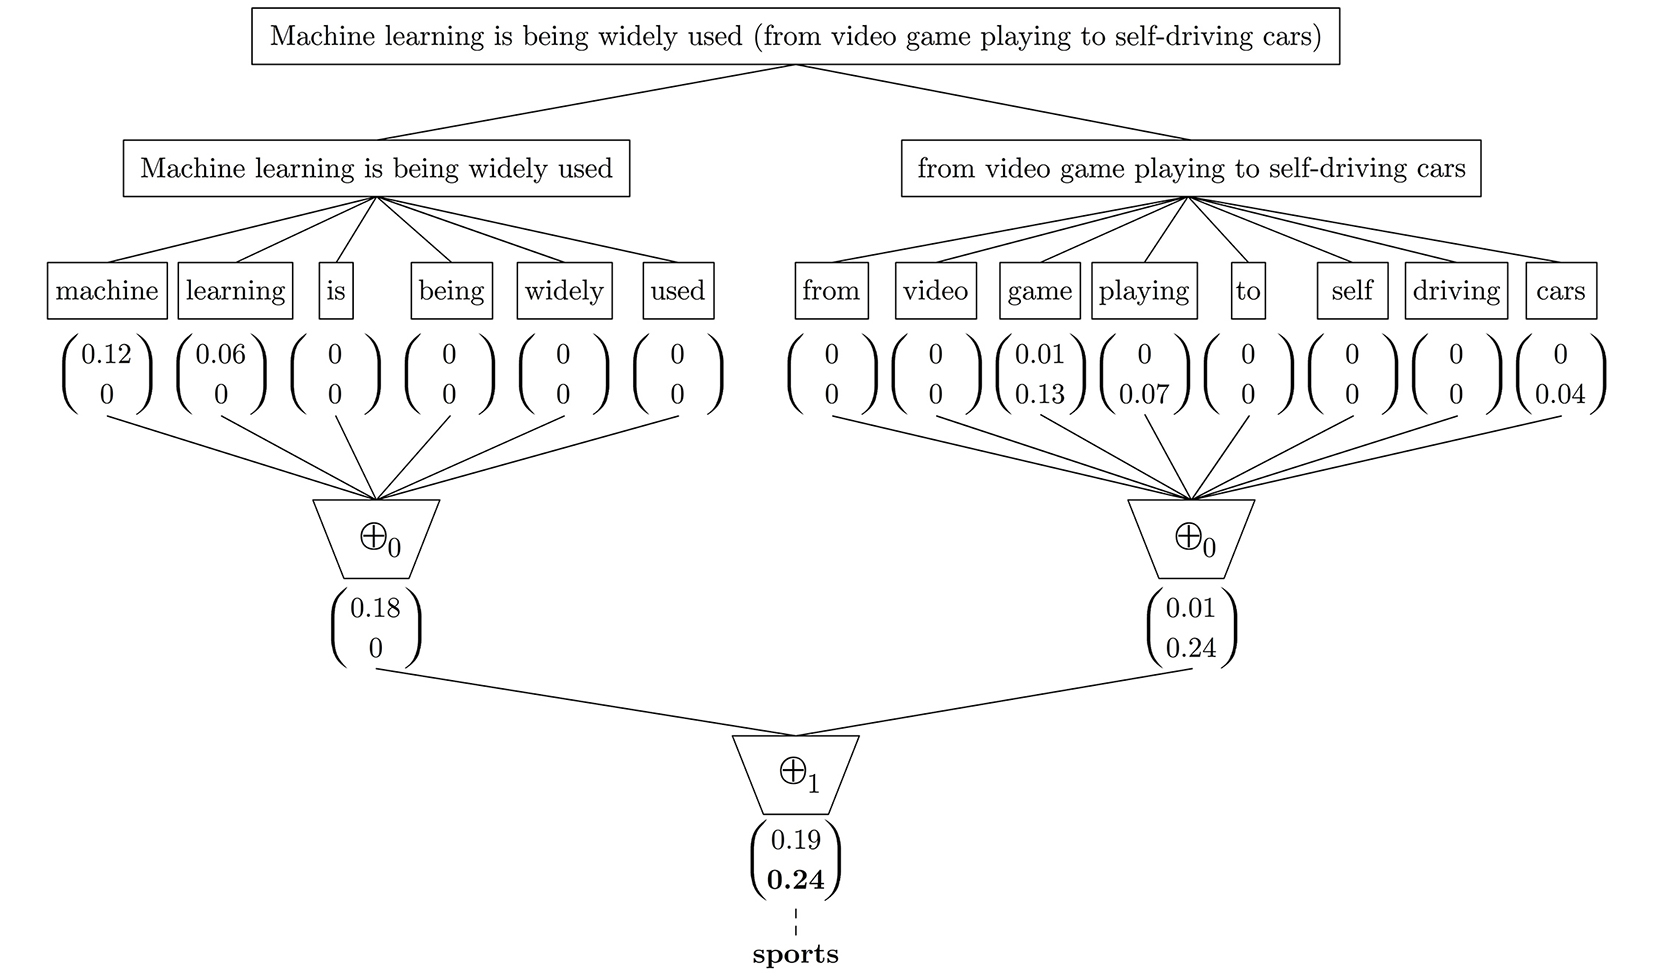
\includegraphics[width=190mm]{images/ss3-machine-learning}}
    \caption{
    Ejemplo de clasificación para las clases \emph{technology} y \emph{sports}.
    En este ejemplo, SS3 clasificó de forma incorrecta la temática del documento como \emph{sports}, ya que no puede capturar secuencias importantes para \emph{technology} como ser \emph{``machine learning''} o \emph{``video game''}.
    Esto se debe a que cada oración fue procesada como una bolsa de palabras.}
    % Classification example for categories \emph{technology} and \emph{sports}. In this example, SS3 misclassified the document's topic as $sports$ since it failed to capture important sequences for \emph{technology} like \emph{``machine learning''} or \emph{``video game''}. This was due to each sentence being processed as a bag of words.}
    \label{fig:ss3-example}
\end{figure*}

Una de las formas habituales para intentar mitigar algunas de las limitaciones de la representación de bolsa de palabras es identificar a los términos con n-gramas de palabras. De esta forma, el modelo mantiene, en cada término, alguna noción local del orden de las palabras de la entrada original.
% Las debilidades de las representaciones de bolsa de palabras son bien conocidas en el campo de clasificación de documentos tradicional, en el que generalmente se usan n-gramas de palabras para intentar remediarlas.
Desafortunadamente, cuando la entrada es una secuencia, en nuestro caso un flujo virtualmente infinito de texto, el uso de los n-gramas de palabras no es trivial, ya que, idealmente, los sistemas tienen que aprender a identificar dinámicamente qué n-gramas son los importantes ``sobre la marcha''.
% The weaknesses of bag-of-words representations are well-known in the standard document classification field, in which word n-grams are usually used to overcome them.
% Unfortunately, when dealing with text streams, using word n-grams is not a trivial task since the system has to dynamically identify, create and learn which n-grams are important ``on the fly''.
En este capítulo introducimos una generalización de SS3, llamada $\tau$-SS3, que expande su definición original permitiéndole el reconocimiento de secuencias de palabras importantes, sin que esto implique perder ninguna de sus cualidades originales: \emph{
entrenamiento y clasificación incremental}, \emph{clasificación anticipada} y \emph{transparencia/explicabilidad}.
Así, en la \autoref{sec:tss3} se introduce formalmente la expansión del modelo, describiendo los algoritmos y ecuaciones necesarias, y en la \autoref{sec:tss3-results} se evalúa el modelo, no sólo en la tarea eRisk 2017 como en el capítulo anterior, sino también en dos nuevas tareas, detección anticipada de anorexia y detección anticipada de depresión del eRisk 2018.
% Finalmente, la \autoref{sec:tss3-conclusion} resume las conclusiones principales derivadas de este capítulo.
% In this paper, we introduce a variation of SS3, called $\tau$-SS3, which expands its original definition to allow recognizing important word sequences.
% In \autoref{sec:ss3} the original SS3 definition is briefly introduced. 
% \autoref{sec:tss3} formally introduces $\tau$-SS3, in which the needed equations and algorithms are described.
% In \autoref{sec:results} we evaluate our model on the CLEF's eRisk 2017 and 2018 tasks on early depression and anorexia detection.
% Finally, \autoref{sec:conclusion} summarizes the main conclusions derived from this work.

\section{El Modelo de Clasificación de Texto \texorpdfstring{$\tau$}{t}-SS3}
\label{sec:tss3}

En esta sección describimos cómo expandir el modelo SS3 para permitirle operar sobre secuencias de palabras, por lo que primero se examinará simplemente el aspecto formal de dicha expansión, y luego se abordará cómo es posible llevarla  efectivamente a la práctica, tanto para el entrenamiento como para la clasificación.

\

Así, en relación a la definición formal de la expansión del modelo, el único cambio que necesitamos introducir es una versión generalizada de la función $lv$ dada en \autoref{eq:lv-first}. Esta generalización es trivial ya que sólo implica permitir que $lv$ valore no sólo palabras, sino también secuencias de palabras.
Es decir, en símbolos, si $t_k = w_1 {\rightarrow} w_2 \dots {\rightarrow} w_k$ es una secuencia de $k$ palabras, entonces ahora definiremos a $lv$ como:
% Regarding the model's formal definition, the only change we need to introduce is a generalized version of the $lv$ function given in \autoref{eq:lv-p}. This is trivial because it only involves allowing $lv$ to value not only words but also sequences of them. That is, in symbols, if $t_k = w_1{\rightarrow}w_2\dots{\rightarrow}w_k$ is a sequence of $k$ words, then $lv$ is now defined as:

\begin{equation}
\label{eq:t-lv-p}
lv_\sigma(t_k, c) = \bigg(\frac{P(w_1w_2\dots w_k|c)}{P(m_1m_2\dots m_k|c)}\bigg)^\sigma
\end{equation}

\vspace{5mm}

Donde, de manera análoga a la definición original, $m_1m_2\dots m_k$ es la secuencia con la máxima probabilidad de ocurrencia, bajo el supuesto que la clase es $c$.
% where $m_1m_2\dots m_k$ is the sequence of $k$ words with the highest probability of occurring given that the category is $c$.

\

Luego, al igual que con la \autoref{eq:lv-fr}, la definición final de $lv$, en término de las frecuencias almacenadas durante el entrenamiento, se vuelve:
% Then, as with \autoref{eq:lv}, the actual definition of $lv$ becomes:

\begin{equation}
lv_\sigma(t_k, c) = \bigg(\frac{tf_{t_k,c}}{max\ tf_{k,c}}\bigg)^\sigma
\label{eq:t-lv}
\end{equation}

\vspace{5mm}
% \

Donde $tf_{t_k,c}$ denota la frecuencia de la secuencia $t_k$ en $c$ y $max\{tf_{k,c}\}$ la frecuencia máxima vista en $c$ para secuencias de largo $k$.
% Where $tf_{t_k,c}$ denotes the frequency of sequence $t_k$ in $c$ and $max\{tf_{k,c}\}$ the maximum frequency seen in $c$ for sequences of length $k$.

\vspace{5mm}

Así, dada cualquier secuencia de palabras $t_k$, en principio, ahora podríamos calcular su valor global, $gv(t_k, c)$, utilizando la definición original de $gv$, presentada en la \autoref{eq:gv}.
Por ejemplo, supongamos que $\tau$-SS3 ha aprendido que las siguientes secuencias de palabras tienen los siguientes valores $gv$:
% Thus, given any word sequence $t_k$, now we could use the original \autoref{eq:gv} to compute its $gv(t_k, c)$. For instance, suppose $\tau$-SS3 has learned that the following word sequences have the $gv$ value given below:

\

\begin{tabular}{ll} %p{0.5\linewidth}}
$gv(machine{\rightarrow}learning, technology) = 0.23;$\\
$gv(video{\rightarrow}game, technology) = 0.19;$\\
$gv(self{\rightarrow}driving{\rightarrow}cars, technology) = 0.21;$\\
\end{tabular}

\vspace{5mm}


\begin{figure*}[t!]
    \centering
    \centerline{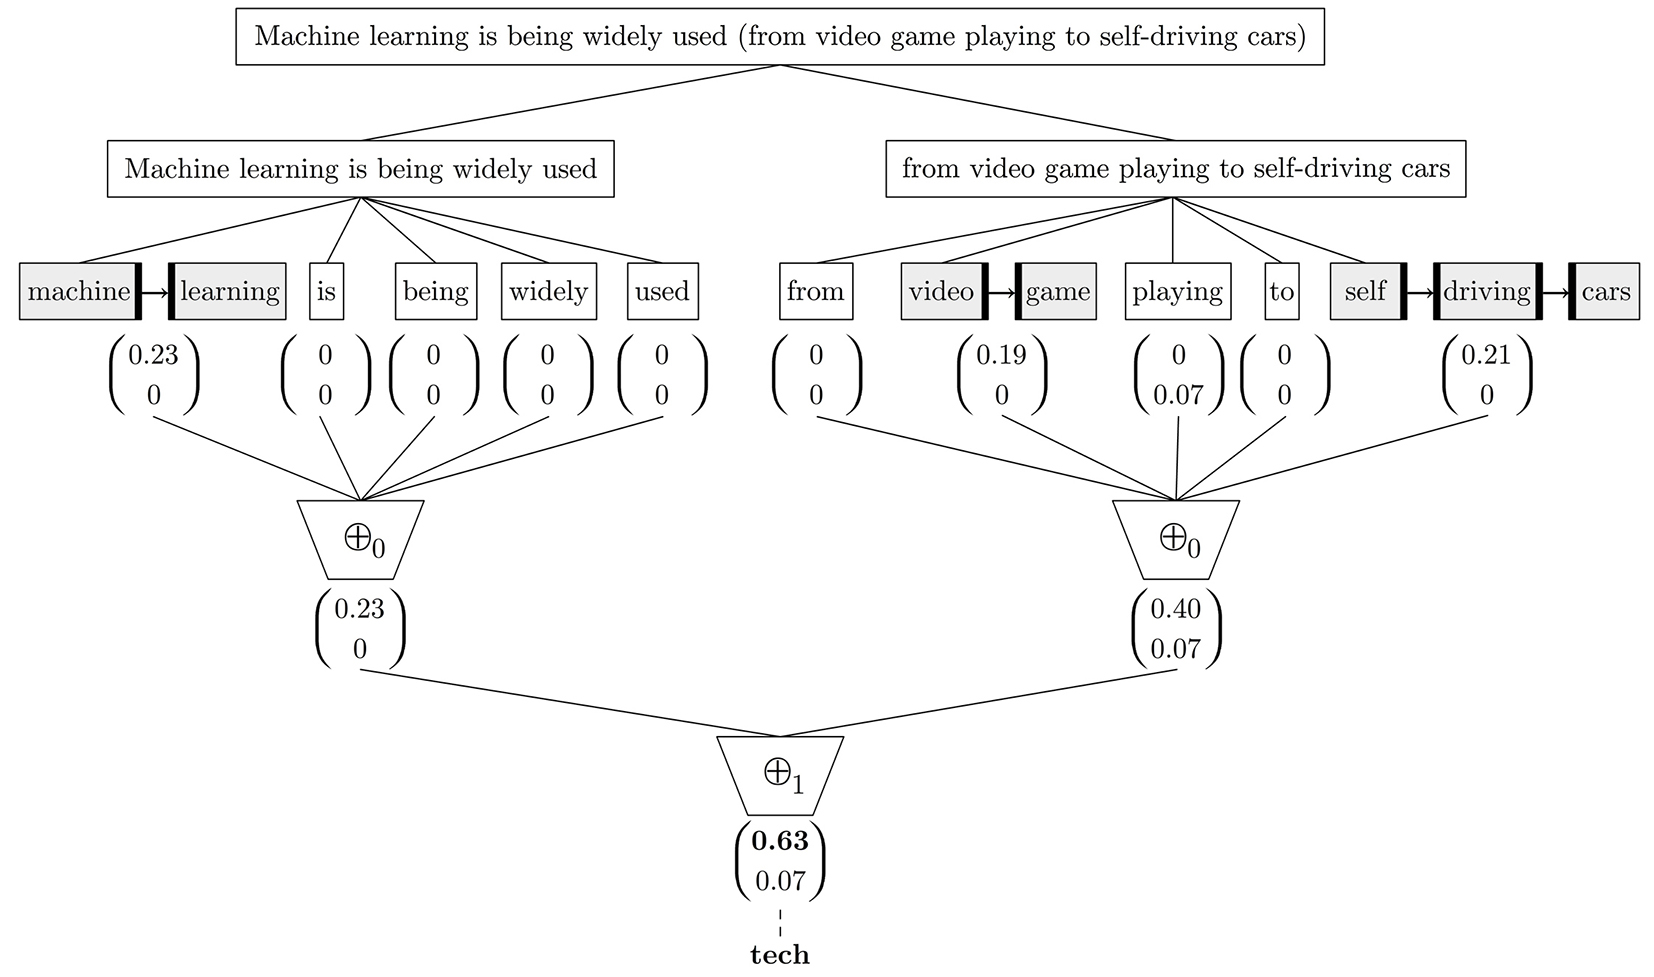
\includegraphics[width=190mm]{images/t-ss3-machine-learning}}
    \caption{
    Ejemplo de clasificación con $\tau$-SS3. Ya que SS3 ahora tiene la capacidad de valorar secuencias de palabras, esta vez fue capaz de clasificar correctamente la temática del documento como \emph{technology}.}
    % $\tau$-SS3 classification example. Since SS3 now has the ability to capture important word sequences, it is able to correctly classify the document's topic as $tech$.}
    \label{fig:t-ss3-example}
\end{figure*}


Luego, el ejemplo de clasificación incorrecta mostrado anteriormente en la \autoref{fig:ss3-example} podría clasificarse de forma correcta utilizando estos nuevos valores, como se ilustra en la \autoref{fig:t-ss3-example}.
En las siguiente sección, veremos cómo se podría implementar esta extensión formal en la práctica. Es decir, cómo podríamos implementar los algoritmos de aprendizaje y clasificación para, respectivamente, almacenar las secuencias aprendidas y reconocer estas secuencias importantes, dinámicamente, durante la clasificación.
% Then, the previously misclassified example could now be correctly classified, as shown in \autoref{fig:t-ss3-example}.
% In the following subsections, we will see how this formal extension is, in fact, implemented in practice. %, i.e., how the training and classification algorithms are implemented to store the learned sequences and to, in fact, dynamically recognize sequences like those of this example during classification time.


\subsection{Entrenamiento}


El algoritmo de aprendizaje original sólo necesitaba un diccionario de pares palabra-frecuencia por cada clase.
Luego, cada diccionario se actualizaba a medida que se procesaban nuevos documentos de entrenamiento, agregando nuevas palabras al diccionario y actualizando la frecuencia de las ya almacenadas.
Estas frecuencias eran el único elemento que se necesitaba guardar ya que era lo único necesario para calcular $lv(w,c)$.
% The original SS3 learning algorithm only needs a dictionary of term-frequency pairs for each category.
% Each dictionary is updated as new documents are processed ---i.e., unseen terms are added and frequencies of already seen terms are updated.
% Note that these frequencies are the only elements we need to store since to compute $lv(w,c)$ we only need to know $w$'s frequency in $c$, $tf_{w,c}$ (see \autoref{eq:lv}).

\begin{algorithm}[t]
\small
\caption{\small Nuevo algoritmo de aprendizaje. Redefinición de la función \textproc{Aprender-Documento} del \autoref{alg:training} original (véase página \pageref{alg:training}). Notar que aquí $texto$ es una secuencia de unidades léxicas que incluye no sólo palabras sino también signos de puntuación. $MAX\_NIVEL$ almacena el tamaño máximo permitido de secuencia.}
% Learning Algorithm. Note that $text$ is a sequence of lexical units (terms) which includes not only words but also punctuation marks.  $MAX\_NIVEL$ stores the maximum allowed sequence length.}
\label{alg:t-ss3-training}
\begin{algorithmic}[1]
\Statex
\Procedure{Aprender-Documento}{$texto$, \emph{etiqueta}}
	\State \Input $texto$, una secuencia de unidades léxicas del documento
	\State \inputindent \emph{etiqueta}, la etiqueta de la clase a la que pertenece el documento
	\State \LocalVariables $cursores$, un conjunto de nodos del árbol de prefijos
	\State
	\State \Call{Árbol-De-Prefijos}{} $\gets$ el árbol correspondiente a la clase dada por \emph{etiqueta}
	\State $cursores$ $\gets$ conjunto vacío
	\For{\emph{término} \In $texto$}
		\If{\emph{término} \textbf{no es} una palabra}
			\State $cursores$ $\gets$ conjunto vacío
		\Else
		    \State agregar \Call{Árbol-De-Prefijos}{}.\Call{Raíz}{} a $cursores$
		    \For{$nodo$ \In $cursores$}
		        \If{$nodo$ \textbf{no} tiene un hijo para \emph{término}}
		            \State $nodo$.\Call{Nodo-Hijo}{}.\Call{nuevo}{\emph{término}}
		        \EndIf
		        \State $nodo\_hijo$ $\gets$ $nodo$.\Call{Nodo-Hijo}{}[\emph{término}]
		        \State $nodo\_hijo$.\Call{Frecuencia}{} $\gets$ $nodo\_hijo$.\Call{Frecuencia}{} + 1
		        \If{$nodo\_hijo$.\Call{Nivel}{} $\ge$ $MAX\_NIVEL$}
		            \State remover $nodo$ de $cursores$
		        \Else
		            \State reemplazar $nodo$ con $nodo\_hijo$ en $cursores$
		        \EndIf
		    \EndFor
		\EndIf
	\EndFor
\EndProcedure
\end{algorithmic}
\end{algorithm}

Del mismo modo, el nuevo algoritmo de aprendizaje para $\tau$-SS3 sólo necesita almacenar las frecuencias de todas las secuencias de palabras observadas en los documentos de entrenamiento.
% Likewise, $\tau$-SS3 learning algorithm only needs to store frequencies of all word sequences seen while processing training documents.
Más precisamente, dado un entero positivo $n$, necesitamos almacenar la frecuencia de todos los $k$-gramas de palabras observados durante el entrenamiento, con $1 \leq k \leq n$ ---es decir, palabras individuales, bigramas, trigramas, y así.
% More precisely, given a fixed positive integer $n$, it must store information about all word $k$-grams seen during training, with $1 \leq k \leq n$ ---i.e., single words, bigrams, trigrams, etc.
Para llevar esto a cabo, el nuevo algoritmo, dado en \autoref{alg:t-ss3-training}, utiliza un \emph{árbol de prefijos}\footnote{A esta estructura de datos también se la conoce como \emph{trie}.} \cite{trie1960, crochemore2009trie} para almacenar todas las frecuencias.
% To achieve this, the new learning algorithm uses a \emph{prefix tree} (also called \emph{trie})\cite{trie1960, crochemore2009trie} to store all the frequencies, as shown in \autoref{alg:training}.
Notar que, en lugar de haber utilizado $k$ diferentes diccionarios por cada clase para almacenar los distintos $k$-gramas (\emph{e.g.} uno para palabras, otro para bigramas, otro para trigramas, y así), se ha decidido utilizar un único \emph{árbol de prefijos}, ya que todos los n-gramas siempre serán prefijos de los n-gramas más largos.\footnote{Por ejemplo, ``Don'' es prefijo de ``Don Quijote``, que a su vez es prefijo de ``Don Quijote de'', prefijo de ``Don Quijote de la'', que finalmente es prefijo de ``Don Quijote de la Mancha''.}
% Note that instead of having $k$ different dictionaries, one for each $k$-grams (e.g. one for words, one for bigrams, etc.) we have decided to use a single prefix tree since all n-grams will share common prefix with the shorter ones.
Además, en lugar de procesar el documento de entrada $k$ veces, nuevamente, una vez por cada tipo de $k$-gramas, se han decidido utilizar $k$ múltiples cursores sobre un mismo árbol. Estos cursores permiten que se puedan almacenar los distintos $k$-gramas, en simultáneo y de corrida, a medida que se va procesando la secuencia de entrada en flujo.
% Additionally, note that instead of processing the input document $k$ times, again one for each $k$-grams, we have decided to use multiple cursors to be able to simultaneously store all sequences allowing the input to be processed as a stream.
Finalmente, para no desperdiciar espacio de almacenamiento, notar que las líneas 8 y 9 del \autoref{alg:t-ss3-training} aseguran que sólo se tengan en cuenta n-gramas que, en principio, ``tengan sentido'', es decir, aquellos que estén formados solamente por palabras ---\emph{i.e.} que no tengan símbolos de puntuación en el medio.
% Finally, note that lines 8 and 9 of \autoref{alg:t-ss3-training} ensure that we are only taking into account n-grams that make sense, i.e., those composed only of words.
Todas estas observaciones previas, así como también la intuición del algoritmo, son ilustradas con un sencillo ejemplo en la \autoref{fig:t-ss3-training}.
% All these previous observations, as well as the algorithm intuition, are illustrated with an example in \autoref{fig:t-ss3-training}.
Este ejemplo asume que el entrenamiento recién  ha comenzado por primera vez, y que el primer documento a ser procesado es la pequeña oración \emph{``Mobile APIs, for mobile developers''} 
% This example assumes that the training has just begun for the first time and that the short sentence, \emph{``Mobile APIs, for mobile developers''}, is the first document to be processed.
---por lo que el árbol continuará creciendo luego, a medida que nuevos documentos de entrenamiento sean procesados.
% Note that this tree will continue to grow, later, as more documents are processed.

\begin{figure*}[t]
    \centering
    \centerline{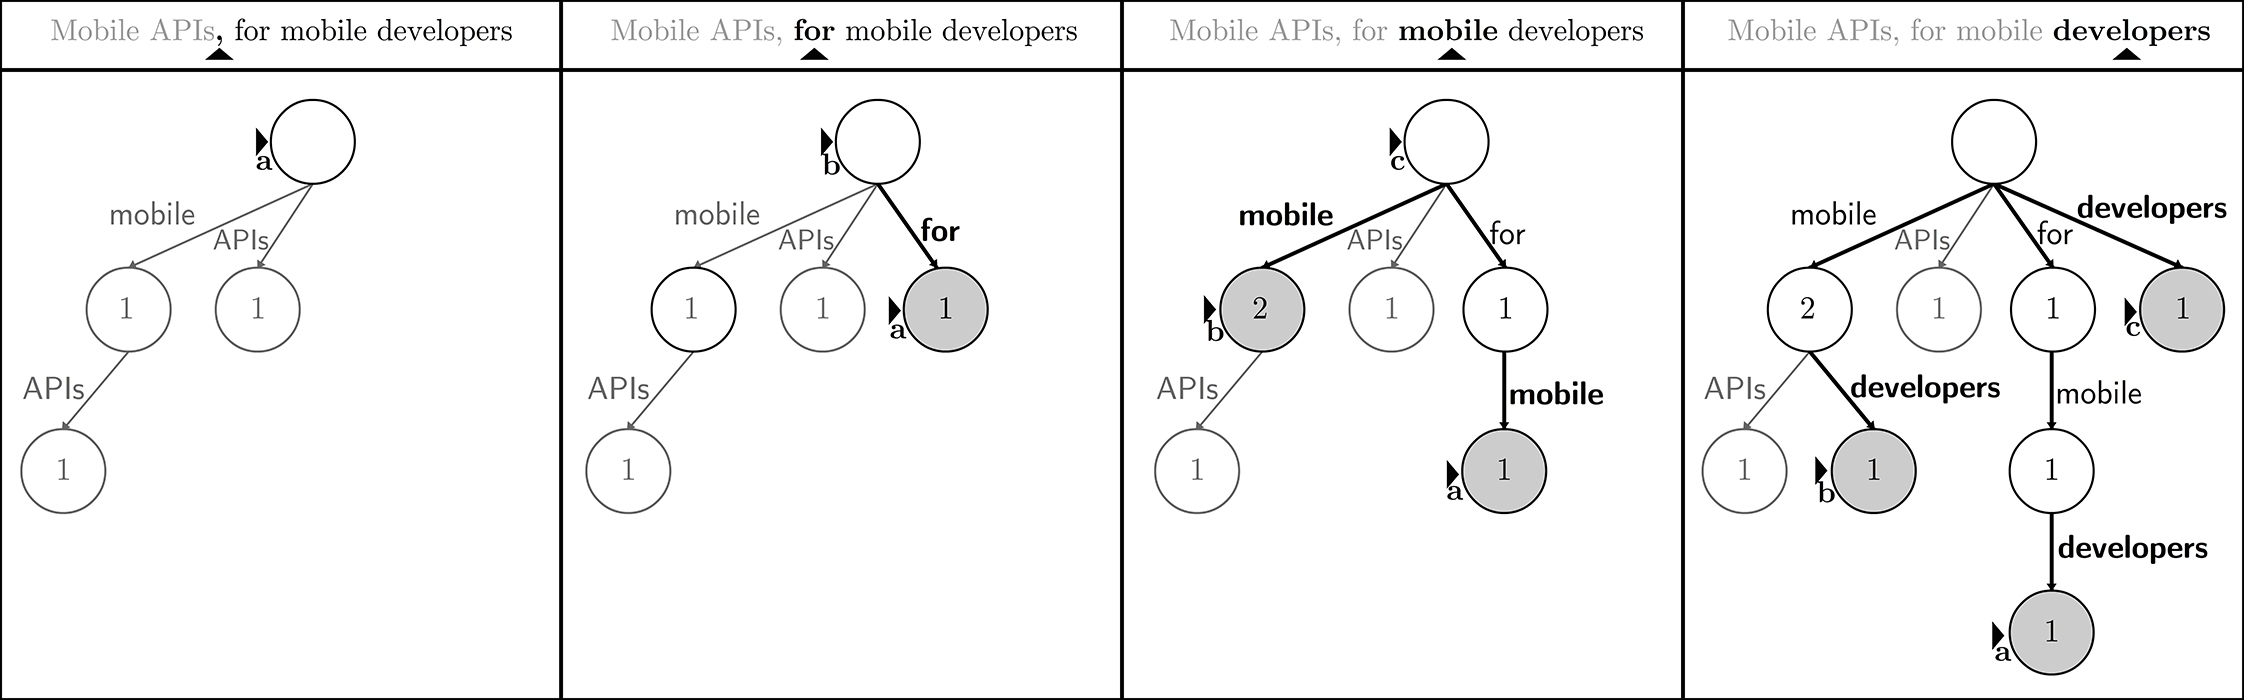
\includegraphics[width=190mm]{images/trie-training}}
    \caption{Ejemplo del proceso de entrenamiento. Las actualizaciones son indicadas con el color gris y la negrita.
    (a) las primeras dos palabras han sido consumidas y, por lo tanto, en el árbol se crearon tres nodos, uno para cada palabra y uno para el bigrama ``mobile APIs'', luego, en la entrada se encontró una coma, lo que provocó que se removieran todos los cursores y que se ubicara uno nuevo, $a$, apuntando a la raíz (véase líneas 9 y 10 del \autoref{alg:training});
    (b) se avanza una posición el cursor de entrada y se consume la palabra ``for'', se crea un nuevo nodo para esta palabra utilizando al cursor $a$ (véase línea 14), el cual luego se actualiza para apuntar a este nuevo nodo (línea 15 y 20) y un nuevo cursor $b$ es creado (línea 11) apuntando a la raíz;
    (c) se consume una nueva palabra desde la entrada, ``mobile'', usando el cursor $b$, se actualiza el nodo para esta palabra incrementando su frecuencia a 2 (línea 16). Además, un nuevo nodo es creado para el bigrama ``for mobile'' usando el antiguo cursor $a$ y, nuevamente, un nuevo cursor $c$ es creado para el nodo raíz (línea 11);
    (d) finalmente, se consume la palabra ``developers'' y, similarmente, nuevos nodos son creados para dicha palabra, el bigrama ``mobile developers'' y el trigrama ``for mobile developers''.}
    % Training example. Gray color and bold indicate an update.
    % (a) the first two words have been consumed and the tree has 3 nodes, one for each word and one for the bigram ``mobile APIs'', then a comma (,) is found in the input and \autoref{alg:training}'s line 9 and 10 have removed all the cursors and placed a new one, $a$, pointing to the root;
    % (b) the word ``for'' is consumed, a new node for this word is created using the node pointed by cursor $a$ (lines 14), $a$ is updated to point to this new node (line 15 and 20), the next term is read and a new cursor $b$ is created (line 11) in the root;
    % (c) ``mobile'' is consumed, using cursor $b$ the node for this word updated its frequency to 2 (line 16), a new node is created for the bigram ``for mobile'' using cursor $a$, and a new cursor $c$ is created in the root node (line 11);
    % (d) finally, the word ``developers'' is consumed and similarly, new nodes are created for word ``developers'', bigram ``mobile developers'' and trigram ``for mobile developers''.}
    \label{fig:t-ss3-training}
\end{figure*}

De esta forma, cada clase tendrá un \emph{árbol de prefijos} almacenando información relacionada a las distintas secuencias de palabras, habiendo así un nodo en el árbol por cada k-grama aprendido.
% Thus, each category has a \emph{prefix tree} storing information linked to word sequences in which there is a tree's node for each learned k-gram.
Notar que en el \autoref{alg:t-ss3-training}, nunca habrá más de $MAX\_NIVEL$ cursores y que, de igual manera, la altura de cada árbol nunca podrá ser mayor a $MAX\_NIVEL$, ya que los nodos del nivel 1 almacenarán unigramas, a nivel 2 bigramas, nivel 3 trigramas, y así sucesivamente.
% Note that in \autoref{alg:training}, there will never be more than $MAX\_LVL$ cursors and that the height of the trees will never grow higher than $MAX\_LVL$ since nodes at level 1 store 1-grams, at level 2 store 2-gram, and so on.
Finalmente, cabe destacar que este nuevo algoritmo de aprendizaje también nos permite conservar la principal virtud del original.
Esto es, el entrenamiento sigue siendo incremental\footnote{Es decir, el modelo sigue soportando \emph{online learning}.} ya que no hay necesidad de almacenar todos los documentos ni tener que reentrenar desde cero cada vez que se dispongan de nuevos documentos de entrenamiento, en su lugar, sólo será necesario actualizar los árboles ya existentes, creando nuevos nodos o actualizando las frecuencias.
% Finally, it is worth mentioning that this learning algorithm allows us to keep the original one's virtues. Namely, the training is still incremental (i.e., it supports online learning) since there is no need neither to store all documents nor to re-train from scratch every time new training documents are available, instead, it is only necessary to update the already created trees.
% Additionally, there is still no need to compute the document-term matrix because, during classification and using \autoref{eq:t-lv} and \autoref{eq:gv}, $gv$ could be dynamically computed based on the frequencies stored in the trees.

\subsection{Clasificación}

\begin{figure}[t!]
    \begin{subfigure}{0.5\textwidth}
        \centering
        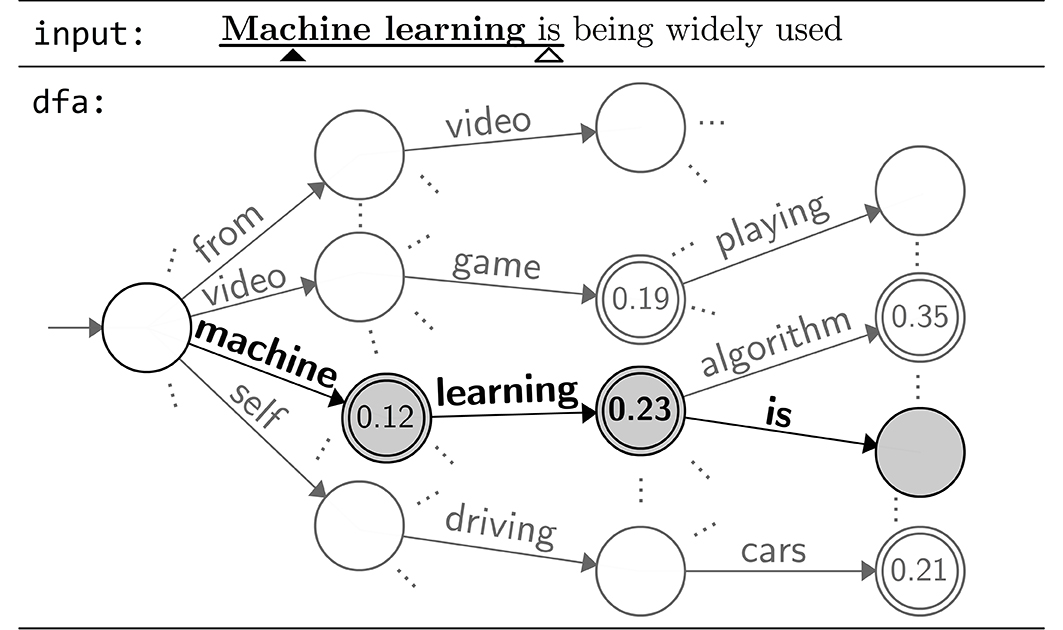
\includegraphics[width=\textwidth]{images/dfa0}
        \caption{}
        \label{fig:dfa_a}
    \end{subfigure}
    \begin{subfigure}{0.5\textwidth}
        \centering
        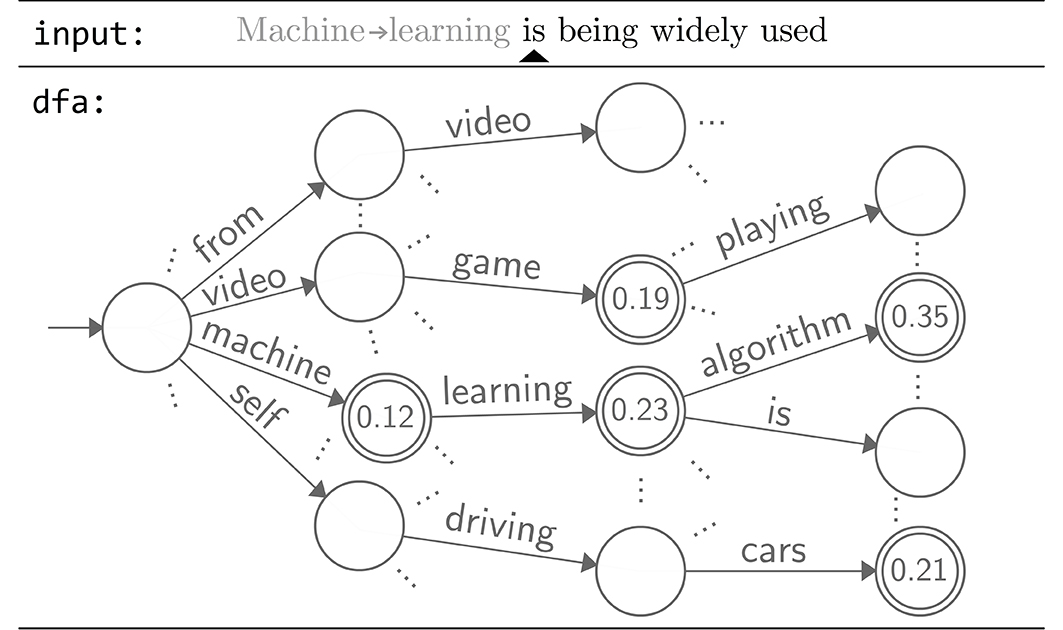
\includegraphics[width=\textwidth]{images/dfa1}
        \caption{}
        \label{fig:dfa_b}
    \end{subfigure}
\caption{Ejemplo de reconocimiento del mejor n-grama para la oración ``Machine learning is being widely used'', perteneciente al primer bloque oración del ejemplo de la \autoref{fig:t-ss3-example}.
% Example of recognizing the best n-gram for the first sentence block of \autoref{fig:t-ss3-example}, ``Machine learning is being widely used''.
Por simplicidad, en esta figura sólo se muestra el \ac{AFD} de \emph{technology}.
% For simplicity in this example, we only show the  \emph{technology}'s DFA.
Conceptualmente hay 2 cursores, uno negro ($\blacktriangle$) y uno blanco ($\vartriangle$). El primero, llamado ``cursor de entrada'', apunta al próximo término a ser consumido de la oración de entrada. El segundo, llamado ```cursor de búsqueda'', es el que se utiliza para alimentar a los autómatas con el fin de buscar/obtener el mejor n-grama. 
% There are conceptually 2 cursors, the black one ($\blacktriangle$) represents the input cursor and the white one ($\vartriangle$) the ``lookahead'' cursor to feed the automatons.
(a) El cursor de búsqueda ha avanzado alimentando al AFD con 3 palabras (``machine'', ``learning'', e ``is'') hasta que no hubo ninguna otra transición válida.
% (a) The lookahead cursor has advanced feeding the DFA with 3 words (``machine'', ``learning'', and ``is'') until no more state transitions were available.
En este punto, hay dos posibles estados finales, uno para ``machine'' y otro para ``machine learning'', seleccionándose este último por tener el mayor valor $gv$ (0.23);
% There were two possible final states, one for ``machine'' and another for ``machine$\rightarrow{}$learning'', the latter is selected since it has the highest $gv$ (0.23);
(b) Finalmente, luego de que el bigrama ``machine learning'' haya sido reconocido  y seleccionado, el cursor de entrada avanza 2 posiciones y está listo para comenzar el proceso de reconocimiento nuevamente, esta vez con ``is'' como la primer palabra para alimentar a los autómatas.}
% (b) Finally, after the bigram ``machine$\rightarrow{}$learning'' was recognized (see the first two word blocks painted in gray in \autoref{fig:t-ss3-example}), the input cursor advanced 2 positions and is ready to start the process again using ``is'' as the first word to feed the automatons.}
\label{fig:dfa}
\end{figure}

El nuevo algoritmo de clasificación será en gran medida el mismo que el original, dado en el \autoref{alg:classification} (véase página \pageref{alg:classification}), sólo será necesario cambiar el proceso por el cual las oraciones son divididas en palabras individuales, para permitir que sean divididas de forma más inteligente en secuencias de una o más palabras,
% The original classification algorithm will remain mostly unchanged\footnote{See Algorithm 1 from the original work \cite{burdisso2019}.}, we only need to change the process by which sentences are split into single words, by allowing them to be split into variable-length n-grams.
siendo estas secuencias ``las mejores posibles'' ---\emph{i.e.} las que tengan el máximo \emph{valor global}.
% Also, these n-grams must be ``the best possible ones'', i.e., having the maximum $gv$ value.
Para lograr este objetivo, utilizaremos el árbol de prefijos de cada clase para reconocer estas secuencias importantes como si fuera un \emph{\ac{AFD}}.
% To achieve this goal, we will use the prefix tree of each category as a \emph{deterministic finite automaton} (DFA) to recognize the most relevant sequences.
Esto es, virtualmente, cada nodo del árbol será considerado como un estado final del autómata siempre que su valor global\footnote{Más precisamente, el valor global del n-grama asociado a ese nodo.} sea mayor o igual que una constante pequeña dada, $\epsilon$.
% Virtually, every node will we considered as a final state if its $gv$ is greater or equal to a small constant $\epsilon$.
Así, al procesarse una oración, cada \ac{AFD} avanzará su cursor hasta que no pueda aplicar ninguna transición válida, luego, el n-grama asociado al estado final con el mayor valor global será el reconocido como ``la mejor secuencia de palabras''.
% Thus, every DFA will advance its input cursor until no valid transition could be applied, then the state (node) with the highest $gv$ value will be selected.
Para ayudar a visualizar este proceso, en la \autoref{fig:dfa} se lo ilustra con un sencillo ejemplo y en el \autoref{alg:t-ss3-classification} se brinda su algoritmo formal.
% This process is illustrated in more detail in \autoref{fig:dfa}.

\begin{algorithm}[t!]
\small
\caption{\small Algoritmo de clasificación a nivel oración.}
% \textproc{Map} aplica la función $gv$ a cada n-grama en $ngramas$ y devuelve una lista con los vectores resultantes.
% \textproc{Map} applies the $gv$ function to every n-gram in $ngramas$ and returns a list of resultant vectors.
% \textproc{Reduce} reduce $ngramas\_vcs$ a un único vector aplicando acumulativamente el operador $\oplus_{0}$.}
% \textproc{Reduce} reduces $ngramas\_vcs$ to a single vector by applying the $\oplus_{0}$ operator cumulatively.}
\label{alg:t-ss3-classification}
\begin{algorithmic}[1]
\Statex
\Function{Clasificar-Oración}{$texto$} \Returns un \emph{vector de confianza}
	\State \Input $texto$, la secuencia de unidades léxicas de la oración
	\State \LocalVariables $ngramas$, una secuencia de n-gramas de palabras
	\State \localvarsindent $ngramas\_vcs$, vectores de confianza
%  	\State
	\State $ngramas \gets$ \Call{Parsear}{$texto$}
	\State $ngramas\_vcs \gets$ \Call{Map}{}($gv$, $ngramas$)
	\State \Return \Call{Reduce}{}(\Call{$\oplus_{0}$}{}, $ngramas\_vcs$)
\EndFunction
\Statex \hrulefill
\Function{Parsear}{$texto$} \Returns una secuencia de n-gramas de palabras
    \State \Input $texto$, una secuencia de unidades léxicas
    % \State \GlobalVariables $categories$, las clases aprendidas
    \State \LocalVariables $mejor\_ngrama$, un n-grama
    \State \localvarsindent $resultado$, una secuencia de n-gramas
    \State \localvarsindent $mejores$, una lista de n-gramas
    % \State
    \State $cursor \gets$ el primer término de $texto$
    \While{$cursor$ \textbf{no es} vacío}
        \For{$clase$ \In $clases$}
            \State $mejores[clase] \gets$ \Call{Mejor-N-Grama}{$clase$, $cursor$}
        \EndFor
        \State $mejor\_ngrama \gets$ el n-grama con el mayor $gv$ de $mejores$
        \State agregar $mejor\_ngrama$ a $resultado$
        \State avanzar $cursor$ en $texto$ unas $mejor\_ngrama$.\Call{Longitud}{} posiciones
    \EndWhile
    \State \Return $resultado$
\EndFunction
\Statex \hrulefill
\Function{Mejor-N-Grama}{$clase$, \emph{término}} \Returns un n-grama
    \State \Input $clase$, una clase
    \State \inputindent \emph{término}, un cursor apuntando a un término en la oración
    \State \LocalVariables $estado$, un nodo del árbol de prefijos
    \State \localvarsindent $ngrama$, una secuencia de palabras
    \State \localvarsindent $mejor\_ngrama$, una secuencia de palabras
    % \State
    \State \Call{Árbol-De-Prefijos}{} $\gets$ el árbol asociado a la $clase$
    \State $estado \gets$ \Call{Árbol-De-Prefijos}{}.\Call{Raíz}{}
    \State agregar \emph{término} a $ngrama$
    \State $mejor\_ngrama \gets$ $ngrama$
    \While{$estado$ tenga un hijo para \emph{término}}
        \State $estado \gets$ $estado$.\Call{Nodo-Hijo}{}[\emph{término}]
        \State término $\gets$ próxima palabra en la oración
        \State agregar \emph{término} a $ngrama$
        \If{$gv(ngrama, clase) > gv(mejor\_ngrama, clase)$}
            \State $mejor\_ngrama \gets$ $ngrama$
        \EndIf
    \EndWhile
    \State \Return $mejor\_ngrama$
\EndFunction
\end{algorithmic}
\end{algorithm}

Finalmente, para que este proceso pueda ser incluido como parte del algoritmo de clasificación completo de SS3, sólo es necesario modificar la definición de \textproc{Clasificar-a-Nivel}$(texto, n)$ del algoritmo original (\autoref{alg:classification}), de forma tal que, cuando sea llamado con $n \leq 1$, llame a nuestra nueva función, \textproc{Clasificar-Oración}, dada en el \autoref{alg:t-ss3-classification}.
% Finalmente, el algoritmo formal se da en el \autoref{alg:t-ss3-classification}.\footnote{Notar que para que este algoritmo sea incluido como parte del algoritmo de clasificación original de SS3 (\autoref{alg:classification}), sólo necesitamos modificar la definición de \textproc{Clasificar-a-Nivel}$(texto, n)$ de forma tal que, cuando sea llamada con $n \leq 1$, llamará a nuestra nueva función, \textproc{Clasificar-oración}.}
% Finally, the formal algorithm is given in \autoref{alg:t-ss3-classification}.\footnote{Note that for this algorithm to be included as part of the SS3's overall classification algorithm, we only need to modify the definition of \textproc{Classify-At-Level}$(text, n)$ defined in Algorithm 1 of the original paper \cite{burdisso2019} so that, when called with $n \leq 1$, it will call our new function, \textproc{Classify-Sentence}.}
Notar que, de esta forma, en lugar de dividir las oraciones simplemente en palabras individuales, ahora se llamará a la función \textproc{Parsear} (véase  la línea 5),
% Note that instead of splitting the sentences into words simply by using a delimiter, now we are calling a \textproc{Parse} function on line 6.
la cual dividirá la oración ``inteligentemente'' en una lista de n-gramas de longitud variable.
% \textproc{Parse} intelligently splits the sentence into a list of variable length n-grams.
Siendo más precisos, la división se hará en base a la función \textproc{Mejor-N-Grama} (línea 18) que es la encargada de realizar, efectivamente, el proceso ilustrado en la \autoref{fig:dfa}, devolviendo el mejor n-grama para cada clase.
% This is done by calling the \textproc{Best-N-Gram} function on line 20 which carries out the process illustrated in \autoref{fig:dfa} to return the best n-gram for a given category.



\section{Evaluación Experimental}
\label{sec:tss3-results}

En esta sección se cubrirá el análisis experimental tanto de la extensión propuesta como del modelo original, abordando la detección anticipada de depresión, como en el capítulo anterior, más una nueva tarea, la detección anticipada de anorexia.
La siguiente subsección describe brevemente las tareas y los conjuntos de datos utilizados para entrenar y probar los modelos.
En la \autoref{sec:tss3-implementacion} se describen los detalles de implementación.
Finalmente, la \autoref{sec:tss3-result} examina los resultados obtenidos.

\subsection{Tareas y Conjunto de Datos}

La experimentación se condujo sobre tres tareas de detección anticipada de riesgos.
En particular, los modelos fueron evaluados, no sólo en la tarea del eRisk 2017 \cite{losada2017erisk} del capítulo anterior, sino también en dos nuevas tareas: detección anticipada de anorexia y detección anticipada de depresión del eRisk 2018 \cite{losada2018overview}.
% Así, demás como en el capítulo anterior detección anticipada de depresión tanto del eRisk 2017, como en el capítulo anterior, como del eRisk 2018 \cite{losada2017erisk, losada2018overview} y detección anticipada de anorexia eRisk 2018 \cite{losada2018overview}.
% Experiments were conducted on three of the CLEF's eRisk open tasks, namely eRisk 2017 and 2018 early depression detection \cite{losada2017erisk, losada2018overview} and eRisk 2018 early anorexia detection \cite{losada2018overview}.
Estas nuevas tareas también se centran en procesar secuencialmente el contenido publicado por usuarios de Reddit,
% These tasks focused on sequentially processing the content posted by users on Reddit.
por lo que, al igual que en el capítulo anterior, los conjuntos de datos que fueron utilizados en estas tareas consisten en colecciones de publicaciones creadas por un conjunto de usuarios de Reddit. %, los cuales aquí también volverán a referidos como ``sujetos''.
% Thus, the datasets that were used in these tasks are collections of writings (submissions) posted by a subset of Reddit users (referred to as ``subjects'').
Con el fin de comparar los resultados entre los diferentes modelos participantes, nuevamente, los conjuntos de datos fueron divididos en un conjunto fijo de entrenamiento y uno de prueba.
% In order to compare the results among different participants, as usual, each dataset is split into a training set and a test set.
Así, a los modelos se les entregó el conjunto de entrenamiento para entrenar y ajustar sus hiperparámetros antes de la etapa de prueba ---a cada equipo de investigación participante se le permitió utilizar hasta un máximo de cinco modelos distintos.
% Participating research teams were given the training set to train and tune their models offline and were allowed to submit up to five models each.
Para llevar a cabo la fase de prueba, los organizadores del eRisk decidieron, nuevamente, dividir el historial de publicaciones de cada usuario en diez bloques ---por lo que cada bloque contuvo el $10\%$ del historial completo del usuario.
% To carry out the test phase, eRisk organizers divided each user's writing history into 10 chunks.\footnote{Thus, each chunk contained 10\% of the complete user's history.}
Luego, durante la fase de prueba de clasificación anticipada, a los clasificadores se les dio el historial de publicaciones de cada usuario, un bloque a la vez, teniendo que decidir entre clasificar al usuario como positivo o, de lo contrario, esperar al siguiente bloque porque es requerida más información.
% Classifiers were given each user's history, one chunk at a time,
% % After receiving each chunk, classifiers were asked to decide which users were depressed/anorexic
% and after receiving each chunk, they could either classify the user as depressed/anorexic or wait for the next chunk.
% % Once a decision is emitted for a given user, it cannot be changed in later chunks.

Además, como es de esperarse, los modelos tuvieron que tomar la decisión correcta \emph{tan pronto como sea posible}, ya que la medida de evaluación utilizada fue nuevamente la medida \emph{ERDE} que, como sabemos del capítulo anterior, toma en cuenta no sólo la efectividad de la clasificación, sino también la demora en la toma de decisiones.
En particular, se volvieron a utilizar las medidas $ERDE_5$ y $ERDE_{50}$, las cuales toman como tiempo límite para las decisiones, respectivamente, la publicación número $5$ y $50$ de cada usuario.
% Furthermore, models had to make the correct decision \emph{as early as possible} since their performance was measured taking into account not only the effectiveness but also the delay of their decisions.
% Namely, the evaluation metric that was used is called \emph{Early Risk Detection Error} (ERDE).
% In our case, the performance of all participating models was measured using $ERDE_5$ and $ERDE_{50}$.


\subsection{Detalles de Implementación}
\label{sec:tss3-implementacion}
% \subsection{Implementation details}



La implementación de esta nueva versión del modelo fue codificada modificando la implementación original, realizada en el capítulo anterior, incorporándole la nueva versión de los algoritmos de entrenamiento y clasificación.
% La implementación también fue incorporada al paquete PyPI oficial de SS3, llamado PySS3\cite{burdisso2019pyss3}, el cual será introducido en el \autoref{cap:pyss3} y cuyo código fuente está disponible en Github  (\href{https://github.com/sergioburdisso/pyss3}{\url{https://github.com/sergioburdisso/pyss3}}).
% The new model implementation was coded in \emph{Python} using only built-in functions and data structures (such as \emph{dict}, \emph{map} and \emph{reduce} functions, etc.).
% The implementation was added to the official SS3's PyPI package, PySS3\cite{burdisso2019pyss3}, and its source code is available at \href{https://github.com/sergioburdisso/pyss3}{\url{https://github.com/sergioburdisso/pyss3}}.
Durante la experimentación, se fijó la longitud máxima de los n-gramas en $3$ (\emph{i.e.} se fijó $MAX\_LVL = 3$)\footnote{Se hicieron pruebas con diferentes valores, desde 2 hasta 10, pero el mejor desempeño se obtuvo con $MAX\_LVL = 3$.}
% We also fixed the maximum n-gram length to 3 (i.e., we set $MAX\_LVL = 3$).\footnote{We tried using different values, from 2 to 10, but the best performance was obtained with $MAX\_LVL = 3$.}
y, además, para evitar desperdiciar memoria al dejar que los árboles digitales crezcan innecesariamente por la incorporación de ruido, se ejecutó un procedimiento de ``poda de árbol'' cada millón de palabras procesadas durante el entrenamiento. La poda consistió simplemente en la eliminación de todos los nodos (n-gramas) con una frecuencia menor o igual a 10.
% During experimentation, in order to avoid wasting memory by letting the digital trees grow unnecessarily large, every million words a ``pruning'' procedure was executed in which all the nodes with a frequency less or equal than 10 were removed.

\begin{table}[t]
\centering
\caption{Resultados para la tarea de detección anticipada de depresión del eRisk 2017, ordenada por $ERDE_{50}$. Del total de 30 modelos que fueron enviados por los 8 equipos de investigación, aquí sólo se muestran los que obtuvieron el mejor $ERDE_{5}$ y el mejor $ERDE_{50}$ de cada equipo.}
% \caption{Results on the eRisk 2017 ``Early Depression Detection'' task ordered by ERDE$_{50}$ (the lower, the better). A total of 30 models were submitted by 8 research teams. Here we are only showing the model with best $ERDE_5$ and the model with the best $ERDE_{50}$ of each participating team.}
\label{tab:results-d2017}
\begin{tabular}{l | c c}
\hline
Modelo & $ERDE_{5}$ & $ERDE_{50}\blacktriangle$ \\ \hline
\textbf{$\tau$-SS3}$\star$ & \textbf{12.6\%} & \textbf{7.70\%}  \\
\textbf{SS3}$\star$ & \textbf{12.6\%} & 8.12\% \\
UNSLA & 13.66\% & 9.68\%  \\
FHDO-BCSGA & 12.82\% & 9.69\% \\
UArizonaD & 14.73\% & 10.23\% \\
FHDO-BCSGB & 12.70\% & 10.39\% \\
UArizonaB & 13.07\% & 11.63\% \\
UQAMD & 13.23\% & 11.98\% \\
GPLC & 14.06\% & 12.14\% \\
CHEPEA & 14.75\% & 12.26\% \\
LyRE & 13.74\% & 13.74\% \\
\hline
\end{tabular}
\end{table}

% \begin{table}[t]
% \centering
% \caption{Resultados para la tarea de detección anticipada de depresión del eRisk 2017. Del total de 30 modelos que fueron enviados por los 8 equipos de investigación, aquí sólo se muestran los que obtuvieron el mejor $ERDE_{5}$ y el mejor $ERDE_{50}$ de cada equipo.}
% \label{tab:results-d2017}
% \begin{tabular}{l@{}c || l@{}c}
% \hline
% & $ERDE_5\blacktriangle$ & & $ERDE_{50}\blacktriangle$\\ \hline

% \textbf{$\tau$-SS3}$\star$ & \textbf{12.60\%} & \textbf{$\tau$-SS3}$\star$ & \textbf{7.70\%} \\
% \textbf{SS3}$\star$ & \textbf{12.60\%} & \textbf{SS3}$\star$ & 8.12\% \\
% FHDO-BCSGB & 12.70\% & UNSLA & 9.68\%  \\
% FHDO-BCSGA & 12.82\% & FHDO-BCSGA & 9.69\% \\
% UArizonaB & 13.07\% & UArizonaD & 10.23\% \\
% UQAMD & 13.23\% & FHDO-BCSGB & 10.39\% \\
% UNSLA & 13.66\% & UArizonaB & 11.63\% \\
% LyRE & 13.74\% & UQAMD & 11.98\% \\
% GPLC & 14.06\% & GPLC & 12.14\% \\
% UArizonaD & 14.73\% & CHEPEA & 12.26\% \\
% CHEPEA & 14.75\% & LyRE & 13.74\% \\

% \hline
% \hline
% \end{tabular}
% \end{table}

Finalmente, dado que se quiere realizar una comparación directa y justa con el modelo original, se utilizaron los mismos valores de hiperparámetros que en el capítulo anterior.
% Finally, since we wanted to perform a direct (and fair) comparison against the original SS3 model, we decided to use the same hyperparameter values that were used in the SS3 original paper \cite{burdisso2019}.
Por lo tanto, se fijó $\lambda=\rho=1$ y $\sigma= 0.455$, los cuales, como vimos, habían sido originalmente seleccionados aplicando una búsqueda en grilla minimizando la medida $ERDE_{50}$ sobre el conjunto de entrenamiento, usando una \emph{validación cruzada de 4 iteraciones}.
% Therefore, we set $\lambda=\rho=1$ and $\sigma= 0.455$, which were originally selected by applying a grid search to minimize the $ERDE_{50}$ metric over the training data using 4-fold cross-validation.
Además, por los mismos motivos, como \emph{operadores de resumen}, $\oplus_j$, para todo nivel $j$, se volvió a utilizar la suma de vectores.
% Furthermore, as in the original work, vector addition was used as the \emph{summary operator}, $\oplus_j$, for all the levels.
Del mismo modo, se utilizó la misma política de clasificación anticipada, es decir, los usuarios se clasificaron como positivo tan pronto como el \emph{valor de confianza} positivo, acumulado hasta ese momento, fuese mayor que el negativo.
% Likewise, the same policy for early classification was also applied, i.e., users were classified as positive as soon as the positive accumulated \emph{confidence value} exceeded the negative one.
Finalmente, con respecto al preprocesamiento, no se utilizó ningún método especial salvo una simple normalización eliminando los acentos y convirtiendo el texto a minúsculas, al igual que en el capítulo anterior.\footnote{
Se probaron otros métodos como \emph{stemming} y \emph{lemmatization} utilizando el paquete \emph{Natural Language Toolkit} (NLTK) de Python, pero al contrario de lo que esperábamos inicialmente, el rendimiento del modelo se redujo.}
% Regarding preprocessing, as in the original work, no method was used except for simple accents removal, lowercase conversion, and tokenization.\footnote{
% We also tried performing stemming and lemmatization using the Natural Language Toolkit (NLTK), but contrary to what we initially expected, the early classification performance was reduced.
% }
Esta configuración experimental nos aseguró que, fuera de la adición de los nuevos n-gramas de palabras, ningún otro factor pudiera estar influyendo en los resultados obtenidos.



\subsection{Resultados Experimentales}
\label{sec:tss3-result}



\begin{table}[t]
\centering
\caption{Resultados para la tarea de detección anticipada de depresión del eRisk 2018, ordenada por $ERDE_{50}$. Del total de 44 modelos que fueron enviados por los 11 equipos de investigación, aquí sólo se muestran los que obtuvieron el mejor $ERDE_{5}$ y el mejor $ERDE_{50}$ de cada equipo.}
% \caption{Results on the eRisk 2018 ``Early Depression Detection'' task ordered by ERDE$_{50}$ (the lower, the better). A total of 44 models were submitted by 11 research teams. Here we are only showing the model with best $ERDE_5$ and the model with the best $ERDE_{50}$ of each participating team.}
\label{tab:results-d2018}
\begin{tabular}{l | c c}
\hline
Modelo & $ERDE_{5}$ & $ERDE_{50}\blacktriangle$ \\ \hline
\textbf{$\tau$-SS3}$\star$ & 9.48\% & \textbf{6.17\%} \\
\textbf{SS3}$\star$ & 9.54\% & 6.35\%  \\
FHDO-BCSGB & 9.50\% & 6.44\% \\
FHDO-BCSGA & 9.21\% & 6.68\% \\
LIIRB & 10.03\% & 7.09\% \\
PEIMEXC & 10.07\% & 7.35\% \\
UNSLA & \textbf{8.78\%} & 7.39\%  \\
LIIRA & 9.46\% & 7.56\% \\
UQAMA & 10.04\% & 7.85\% \\
LIRMMD & 11.32\% & 8.08\% \\
UDCA & 10.93\% & 8.27\% \\
UPFA & 10.01\% & 8.28\% \\
RKMVERID & 9.97\% & 8.63\% \\
UDCC & 9.47\% & 8.65\% \\
RKMVERIC & 9.81\% & 9.08\% \\
LIRMMA & 10.66\% & 9.16\% \\
TBSA & 10.81\% & 9.22\% \\
TUA1C & 10.86\% & 9.51\% \\
TUA1A & 10.19\% & 9.70\% \\
\hline
\end{tabular}
\end{table}

% SOLO SS3
% \begin{table}[t]
% \centering
% \caption{Resultados para la tarea de detección anticipada de depresión del eRisk 2018, ordenada por $ERDE_{50}$. Del total de 44 modelos que fueron enviados por los 11 equipos de investigación, aquí sólo se muestran los que obtuvieron el mejor $ERDE_{5}$ y el mejor $ERDE_{50}$ de cada equipo.}
% \label{tab:results-d2018}
% \begin{tabular}{l@{}c || l@{}c}
% \hline
% & $ERDE_5\blacktriangle$ & & $ERDE_{50}\blacktriangle$\\ \hline

% UNSLA & \textbf{8.78\%} & \textbf{SS3}$\star$ & \textbf{6.35\%}  \\
% FHDO-BCSGA & 9.21\% & FHDO-BCSGB & 6.44\% \\
% LIIRA & 9.46\% & FHDO-BCSGA & 6.68\% \\
% UDCC & 9.47\% & LIIRB & 7.09\% \\
% FHDO-BCSGB & 9.50\% & PEIMEXC & 7.35\% \\
% \textbf{SS3}$\star$ & 9.54\% & UNSLA & 7.39\%  \\
% RKMVERIC & 9.81\% & LIIRA & 7.56\% \\
% RKMVERID & 9.97\% & UQAMA & 7.85\% \\
% UPFA & 10.01\% & LIRMMD & 8.08\% \\
% LIIRB & 10.03\% & UDCA & 8.27\% \\
% UQAMA & 10.04\% & UPFA & 8.28\% \\
% PEIMEXC & 10.07\% & RKMVERID & 8.63\% \\
% TUA1A & 10.19\% & UDCC & 8.65\% \\
% LIRMMA & 10.66\% & RKMVERIC & 9.08\% \\
% TBSA & 10.81\% & LIRMMA & 9.16\% \\
% TUA1C & 10.86\% & TBSA & 9.22\% \\
% UDCA & 10.93\% & TUA1C & 9.51\% \\
% LIRMMD & 11.32\% & TUA1A & 9.70\% \\

% \hline
% \hline
% \end{tabular}
% \end{table}

% \begin{table}[t]
% \centering
% \caption{Resultados para la tarea de detección anticipada de depresión del eRisk 2018, ordenada por $ERDE_{50}$. Del total de 44 modelos que fueron enviados por los 11 equipos de investigación, aquí sólo se muestran los que obtuvieron el mejor $ERDE_{5}$ y el mejor $ERDE_{50}$ de cada equipo.}
% \label{tab:results-d2018}
% \begin{tabular}{l@{}c || l@{}c}
% \hline
% & $ERDE_5\blacktriangle$ & & $ERDE_{50}\blacktriangle$\\ \hline

% UNSLA & \textbf{8.78\%} & \textbf{$\tau$-SS3}$\star$ & \textbf{6.17\%} \\
% FHDO-BCSGA & 9.21\% & \textbf{SS3}$\star$ & 6.35\%  \\
% LIIRA & 9.46\% & FHDO-BCSGB & 6.44\% \\
% UDCC & 9.47\% & FHDO-BCSGA & 6.68\% \\
% \textbf{$\tau$-SS3}$\star$ & 9.48\% & LIIRB & 7.09\% \\
% FHDO-BCSGB & 9.50\% & PEIMEXC & 7.35\% \\
% \textbf{SS3}$\star$ & 9.54\% & UNSLA & 7.39\%  \\
% RKMVERIC & 9.81\% & LIIRA & 7.56\% \\
% RKMVERID & 9.97\% & UQAMA & 7.85\% \\
% UPFA & 10.01\% & LIRMMD & 8.08\% \\
% LIIRB & 10.03\% & UDCA & 8.27\% \\
% UQAMA & 10.04\% & UPFA & 8.28\% \\
% PEIMEXC & 10.07\% & RKMVERID & 8.63\% \\
% TUA1A & 10.19\% & UDCC & 8.65\% \\
% LIRMMA & 10.66\% & RKMVERIC & 9.08\% \\
% TBSA & 10.81\% & LIRMMA & 9.16\% \\
% TUA1C & 10.86\% & TBSA & 9.22\% \\
% UDCA & 10.93\% & TUA1C & 9.51\% \\
% LIRMMD & 11.32\% & TUA1A & 9.70\% \\

% \hline
% \hline
% \end{tabular}
% \end{table}

\begin{table}[t]
\centering
\caption{Resultados para la tarea de detección anticipada de anorexia del eRisk 2018, ordenada por $ERDE_{50}$. Del total de 34 modelos que fueron enviados por los 9 equipos de investigación, aquí sólo se muestran los que obtuvieron el mejor $ERDE_{5}$ y el mejor $ERDE_{50}$ de cada equipo.}
% \caption{Results on the eRisk 2018 ``Early Anorexia Detection'' task ordered by ERDE$_{50}$ (the lower, the better). A total of 34 models were submitted by 9 research teams. Here we are only showing the model with best $ERDE_5$ and the model with the best $ERDE_{50}$ of each participating team.}
\label{tab:results-a2018}
\begin{tabular}{l | c c}
\hline
Modelo & $ERDE_{5}$ & $ERDE_{50}\blacktriangle$ \\ \hline
FHDO-BCSGD & 12.15\% & \textbf{5.96\%}  \\
\textbf{$\tau$-SS3}$\star$ & \textbf{11.31\%} & 6.26\%  \\
FHDO-BCSGE & 11.98\% & 6.61\%  \\
\textbf{SS3}$\star$ & 11.56\% & 6.69\% \\
FHDO-BCSGB & 11.75\% & 6.84\%  \\
PEIMEXB & 12.41\% & 7.79\%  \\
UNSLB & 11.40\% & 7.82\%  \\
RKMVERIA & 12.17\% & 8.63\%  \\
LIIRB & 13.05\% & 10.33\%  \\
LIIRA & 12.78\% & 10.47\%  \\
TBSA & 13.65\% & 11.14\%  \\
UPFA & 13.18\% & 11.34\%  \\
UPFD & 12.93\% & 12.30\%  \\
TUA1C & 13.53\% & 12.57\%  \\
LIRMMB & 14.45\% & 12.62\%  \\
LIRMMA & 13.65\% & 13.04\%  \\
\hline
\end{tabular}
\end{table}

% \begin{table}[t]
% \centering
% \caption{Resultados para la tarea de detección anticipada de anorexia del eRisk 2018, ordenada por $ERDE_{50}$. Del total de 34 modelos que fueron enviados por los 9 equipos de investigación, aquí sólo se muestran los que obtuvieron el mejor $ERDE_{5}$ y el mejor $ERDE_{50}$ de cada equipo.}
% \label{tab:results-a2018}
% \begin{tabular}{l@{}c || l@{}c}
% \hline
% & $ERDE_5\blacktriangle$ & & $ERDE_{50}\blacktriangle$\\ \hline

% UNSLB & \textbf{11.40\%} & FHDO-BCSGD & \textbf{5.96\%} \\
% \textbf{SS3}$\star$ & 11.56\% & FHDO-BCSGE & 6.61\% \\
% FHDO-BCSGB & 11.75\% & \textbf{SS3}$\star$ & 6.69\% \\
% FHDO-BCSGE & 11.98\% & FHDO-BCSGB & 6.84\% \\
% FHDO-BCSGD & 12.15\% & PEIMEXB & 7.79\% \\
% RKMVERIA & 12.17\% & UNSLB & 7.82\% \\
% PEIMEXB & 12.41\% & RKMVERIA & 8.63\% \\
% LIIRA & 12.78\% & LIIRB & 10.33\% \\
% UPFD & 12.93\% & LIIRA & 10.47\% \\
% LIIRB & 13.05\% & TBSA & 11.14\% \\
% UPFA & 13.18\% & UPFA & 11.34\% \\
% TUA1C & 13.53\% & UPFD & 12.30\% \\
% TBSA & 13.65\% & TUA1C & 12.57\% \\
% LIRMMA & 13.65\% & LIRMMB & 12.62\% \\
% LIRMMB & 14.45\% & LIRMMA & 13.04\% \\

% \hline
% \hline
% \end{tabular}
% \end{table}

% \begin{table}[t]
% \centering
% \caption{Resultados para la tarea de detección anticipada de anorexia del eRisk 2018, ordenada por $ERDE_{50}$. Del total de 34 modelos que fueron enviados por los 9 equipos de investigación, aquí sólo se muestran los que obtuvieron el mejor $ERDE_{5}$ y el mejor $ERDE_{50}$ de cada equipo.}
% \label{tab:results-a2018}
% \begin{tabular}{l@{}c || l@{}c}
% \hline
% & $ERDE_5\blacktriangle$ & & $ERDE_{50}\blacktriangle$\\ \hline

% \textbf{$\tau$-SS3}$\star$ & \textbf{11.31\%} & FHDO-BCSGD & \textbf{5.96\%} \\
% UNSLB & 11.40\% & \textbf{$\tau$-SS3}$\star$ & 6.26\% \\
% \textbf{SS3}$\star$ & 11.56\% & FHDO-BCSGE & 6.61\% \\
% FHDO-BCSGB & 11.75\% & \textbf{SS3}$\star$ & 6.69\% \\
% FHDO-BCSGE & 11.98\% & FHDO-BCSGB & 6.84\% \\
% FHDO-BCSGD & 12.15\% & PEIMEXB & 7.79\% \\
% RKMVERIA & 12.17\% & UNSLB & 7.82\% \\
% PEIMEXB & 12.41\% & RKMVERIA & 8.63\% \\
% LIIRA & 12.78\% & LIIRB & 10.33\% \\
% UPFD & 12.93\% & LIIRA & 10.47\% \\
% LIIRB & 13.05\% & TBSA & 11.14\% \\
% UPFA & 13.18\% & UPFA & 11.34\% \\
% TUA1C & 13.53\% & UPFD & 12.30\% \\
% TBSA & 13.65\% & TUA1C & 12.57\% \\
% LIRMMA & 13.65\% & LIRMMB & 12.62\% \\
% LIRMMB & 14.45\% & LIRMMA & 13.04\% \\

% \hline
% \hline
% \end{tabular}
% \end{table}

Como se describe con más detalle en la descripción general de cada tarea~\cite{losada2017erisk, losada2018overview} y en las \emph{Working Notes} del CLEF,\footnote{Véase sección ``Early Risk Prediction on the Internet'' de las \emph{Working Notes} del CLEF 2017 (\url{http://ceur-ws.org/Vol-1866/}) y 2018 (\url{http://ceur-ws.org/Vol-2125/}).} entre estas tres tareas del eRisk participaron un total de 180 modelos, los cuales cubren una gran variedad de clasificadores que van desde modelos simples hasta avanzados utilizando enfoques de \emph{aprendizaje profundo}.
% As it is described in more detail in the overview of each task\cite{losada2017erisk, losada2018overview} and the CLEF Working Notes,\footnote{Section ``Early risk prediction on the Internet'' of the CLEF Working Notes for 2017 (\url{http://ceur-ws.org/Vol-1866/}) and 2018 (\url{http://ceur-ws.org/Vol-2125/}).} a total of 180 models were submitted to these three eRisk tasks, ranging from simple to more advanced deep learning models.
Por ejemplo, similar a lo examinado con más detalle el capítulo anterior para la tarea eRisk 2017, en la \autoref{sec:ADD}, algunos grupos de investigación utilizaron clasificadores simples como \ac{MNB}, \ac{RL} o \ac{SVM}, mientras que otros utilizaron métodos más avanzados, tales como diferentes tipos de Redes Neuronales Recurrentes con \emph{embeddings}, distintas arquitecturas de Redes Neuronales Convoluciones, modelos basados en grafos o incluso el ensamble de múltiples clasificadores.
% For instance, some research groups used simple classifiers such as Multinomial Naive Bayes, Logistic Regression, or Support Vector Machine (SVM) while others made use of more advanced methods such as different types of Recurrent Neural Networks with embeddings, graph-based models, or even ensemble of multiple classifiers.

\begin{figure*}[t!]
    \centering
    \begin{subfigure}{0.75\textwidth}
        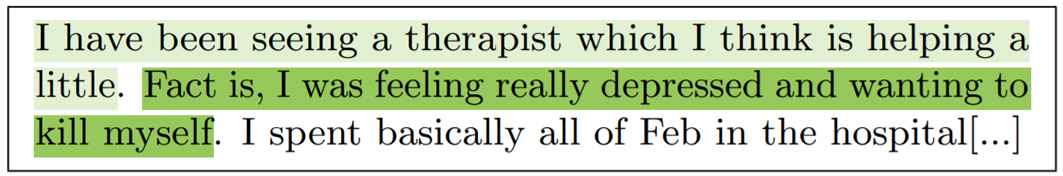
\includegraphics[width=\textwidth]{images/vd-example-a}
        \caption{Explicación a nivel de oración original, dada por SS3}
        \label{fig:subject9579_descriptive_a_tss3}
    \end{subfigure}
    \begin{subfigure}{0.75\textwidth}
        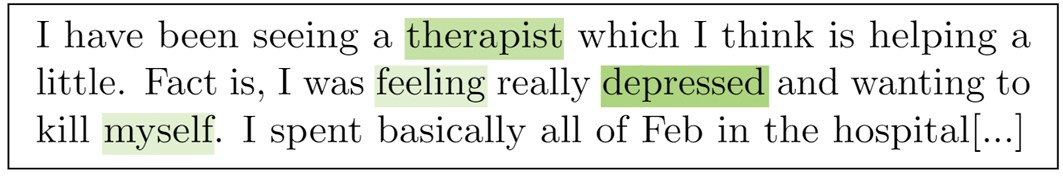
\includegraphics[width=\textwidth]{images/vd-example-c}
        \caption{Explicación a nivel de palabra original, dada por SS3}
        \label{fig:subject9579_descriptive_b_tss3}
    \end{subfigure}
    \begin{subfigure}{0.75\textwidth}
        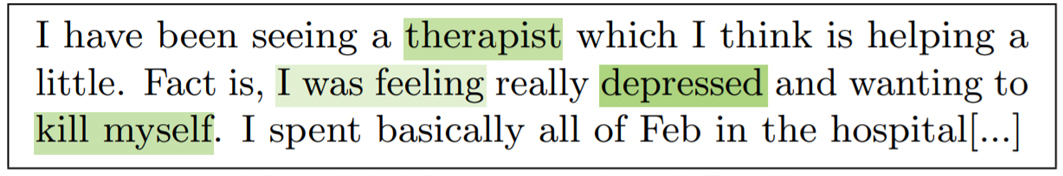
\includegraphics[width=\textwidth]{images/vd-example-b}
        \caption{Nueva explicación a nivel de palabra, dada por $\tau$-SS3}
        \label{fig:subject9579_descriptive_c_tss3}
    \end{subfigure}
\caption{Esta figura muestra un fragmento de la explicación visual dada al final del capítulo anterior. En particular, en (a) y (b) se vuelven a mostrar, respectivamente, las figuras (b) y (c) originales de la \autoref{fig:subject9579_descriptive}, en las que se muestra la publicación número 60 del sujeto 9579 de la tarea eRisk 2017, a dos niveles de explicación (a) oraciones y (b) palabras.
% Los bloques se pintan en relación a los verdaderos \emph{valores de confianza} obtenidos para la clase ``depresivo'' después de la experimentación.
% Esta explicación visual se muestra en dos niveles diferentes: (a) oraciones y (b) palabras.
Además, con fines comparativos, ahora se ha incluido en (c) la nueva explicación visual dada por $\tau$-SS3 para la misma publicación.
Notar que esta nueva explicación resalta información más rica, a saber, el trigrama ``I was feeling'' y el bigrama ``kill myself'', mejorando así la riqueza de las explicaciones visuales.}

% \caption{Esta figura muestra cómo se podría brindar una explicación visual del proceso de clasificación en la tarea abordada. Como mencionamos anteriormente, SS3 nos permite visualizar las razones detrás de la clasificación en diferentes niveles, en nuestro caso: (a) publicaciones, párrafos, (b) oraciones y/o (c) palabras. Cada uno de los segmentos está coloreado en relación al \emph{valor de confianza} positivo, real, obtenido en los experimentos realizados.}

% \caption{This figure shows a fragment of the visual explanation given by SS3 in Figure 9 of the original article \cite{burdisso2019}. It shows the subject 9579's writing 60 of the 2017 depression detection task. Blocks are painted proportionally to the true \emph{confidence values} obtained for the ``\emph{depressed}'' category after experimentation. This visual explanation is shown at two different levels: (a) sentences and (b) words. For comparison purposes, in (c), we now show the new visual explanation given by $\tau$-SS3. Note that more useful information is now shown, namely the trigram ``I was feeling'' and the bigram ``kill myself'', improving the richness of visual explanations.}
\label{fig:subject9579_descriptive_ts33}
\end{figure*}

Los resultados obtenidos para cada una de las tres tareas se muestran, respectivamente, en la \autoref{tab:results-d2017}, \autoref{tab:results-d2018} y \autoref{tab:results-a2018}.
% Results for each one of the three tasks are shown in \autoref{tab:results-d2017}, \autoref{tab:results-d2018}, and \autoref{tab:results-a2018}, respectively.
Como se puede observar, $\tau$-SS3 mejoró ligeramente el desempeño de SS3 en las tres tareas.
% As can be seen, although not significantly, $\tau$-SS3 improves SS3's performance in all three tasks.
Además, $\tau$-SS3 obtuvo los mejores valores de $ERDE_{50}$ para ambas tareas de detección de depresión. Sin embargo, en la tarea de detección de anorexia, obtuvo el segundo mejor valor, por debajo del modelo ``FHDO-BCSGD''~\cite{trotzek2018word}, el cual consiste en una Red Neuronal Convolucional con \emph{embeddings} de palabras obtenidos con \emph{fastText}.
% Furthermore, $\tau$-SS3 obtained the best $ERDE_{50}$ values in both depression detection tasks. However, it obtained the second-best value in the anorexia detection task; the best value was obtained by the FHDO-BCSGD\cite{trotzek2018word} model, which consists of a Convolutional Neural Network (CNN) with \emph{fastText} word embeddings.
En cuanto a $ERDE_{5}$, $\tau$-SS3 también superó a los otros modelos tanto en la tarea de detección de anorexia como en la de detección de depresión del año 2017.
Sin embargo, el mejor valor $ERDE_{5}$ en la tarea de detección de depresión del año 2018 lo obtuvo el modelo ``UNSLA''~\cite{funez2018}, que consiste en un clasificador \ac{SVM} que utiliza una representación de documento especial, denominada ``FTVT'', que tiene en cuenta el aspecto temporal al incorporar información relacionada al número de bloque siendo procesado en el momento.
Vale la pena mencionar que, aunque no se incluyen aquí, el nuevo modelo también mejoró el desempeño original de SS3 en términos de las medidas tradicionales, \emph{precision}, \emph{recall} y $F_1$.
% Regarding $ERDE_{5}$, $\tau$-SS3 also outperformed all the other models in both the anorexia detection and the 2018 depression detection tasks.
% However, the best value in the 2018 depression detection task was obtained by the UNSLA\cite{funez2018} model, which consists of an SVM classifier using a novel (time-aware) document representation, called FTVT.
% It is worth mentioning that, although not included in the tables, the new model also improved the original SS3's performance in terms of the standard (timeless) measures, precision, recall, and $F_1$.
Por ejemplo, en la tarea de detección anticipada de depresión abordada en el capítulo anterior, el \emph{recall}, \emph{precision} y $F_1$ de $\tau$-SS3 fueron $0.55$, $0.43$ y $0.77$, respectivamente, contra $0.52$, $0.44$ y $0.63$ de SS3.
% For instance, in the eRisk 2017 ``Early Depression Detection'' task, $\tau$-SS3's recall, precision and $F_1$ were 0.55, 0.43 and 0.77 respectively, against SS3's 0.52, 0.44 and 0.63.
Además, si bien estos valores no fueron los mejores entre todos los participantes, se situaron bastante por encima del promedio ($0.39$, $0.36$ y $0.51$), lo cual es considerablemente positivo teniendo en cuenta que los valores de hiperparámetros fueron seleccionados para optimizar la medida $ERDE_{50}$.
% Additionally, although these values were not the best among all participants, they were quite above the average (0.39, 0.36, and 0.51), which is not bad considering that our hyperparameter values were selected to optimize the $ERDE_{50}$ measure.

\section{Observaciones Finales}

\begin{table}[t]
\centering
\caption{Top 15 secuencias de una, dos y tres palabras ordenadas por \emph{valor global}, obtenidos para la tarea de detección anticipada de depresión del eRisk 2018.}
\label{tab:ngramas}
\begin{tabular}{l | l | l}
\hline
Unigramas & Bigramas & Trigramas \\ \hline
$depression$ & $my{\rightarrow}boyfriend$ & $i{\rightarrow}m{\rightarrow}feeling$ \\
$anxiety$ & $my{\rightarrow}skin$ & $cerave{\rightarrow}in{\rightarrow}the$ \\
$boyfriend$ & $my{\rightarrow}depression$ & $depression{\rightarrow}and{\rightarrow}anxiety$ \\
$depressed$ & $depression{\rightarrow}and$ & $i{\rightarrow}was{\rightarrow}diagnosed$ \\
$acne$ & $with{\rightarrow}depression$ & $was{\rightarrow}diagnosed{\rightarrow}with$ \\
$meds$ & $anxiety{\rightarrow}and$ & $anxiety{\rightarrow}and{\rightarrow}depression$ \\
$keto$ & $my{\rightarrow}husband$ & $my{\rightarrow}husband{\rightarrow}and$ \\
$cerave$ & $depression{\rightarrow}is$ & $husband{\rightarrow}and{\rightarrow}i$ \\
$makeup$ & $my{\rightarrow}anxiety$ & $a{\rightarrow}panic{\rightarrow}attack$ \\
$routine$ & $my{\rightarrow}pain$ & $my{\rightarrow}boyfriend{\rightarrow}and$ \\
$therapist$ & $panic{\rightarrow}attacks$ & $cerave{\rightarrow}foaming{\rightarrow}cleanser$ \\
$panic$ & $of{\rightarrow}depression$ & $i{\rightarrow}was{\rightarrow}feeling$ \\
$medication$ & $and{\rightarrow}depression$ & $an{\rightarrow}appointment{\rightarrow}with$ \\
$lotion$ & $and{\rightarrow}anxiety$ & $myself{\rightarrow}that{\rightarrow}i$ \\
$nyx$ & $pain{\rightarrow}and$ & $in{\rightarrow}the{\rightarrow}mood$ \\
\hline
\end{tabular}
\end{table}

En este capítulo introdujimos a $\tau$-SS3, una extensión del modelo original presentado en el capítulo anterior. Esta extensión le permite al modelo aprender a reconocer n-gramas de palabras de longitud variable ``sobre la marcha'', a medida que se procesa el texto de entrada ---en otras palabras, esta extensión le brinda al modelo la capacidad de reconocer patrones útiles sobre secuencias de texto.
Vimos que esta extensión fue llevada a la práctica utilizando, por cada categoría, un \emph{árbol de prefijos} para almacenar los n-gramas de longitud variable que se observan durante el entrenamiento y luego, durante la clasificación, esta misma estructura de datos es utilizada como un \emph{autómata finito determinista} que reconoce las secuencias de palabras importantes a medida que se consume la entrada.
Los resultados experimentales mostraron que $\tau$-SS3 superó levemente a SS3 tanto en términos de las medidas de desempeño tradicionales como en las medidas $ERDE_5$ y $ERDE_{50}$, lo que sugiere que los n-gramas aprendidos podrían, en efecto, contribuir positivamente al rendimiento del modelo.
Tal vez una de las causas de esta mejora se deba a que los n-gramas aprendidos, como se ilustra en la \autoref{tab:ngramas}, provocan que palabras previamente ignoradas de forma individual cobren importancia al ser consideradas junto a otras, como es el caso de las palabras ``my'' y ``I'' que predominan en los bigramas y trigramas aprendidos, reflejando el hecho de que el uso de la primera persona es relevante para este tipo de tareas.
Además, y quizás más importante, los n-gramas aprendidos también contribuyen a mejorar la expresividad de las explicaciones visuales dadas por el modelo, como se ilustra en la \autoref{fig:subject9579_descriptive_ts33}.\footnote{Las demos en vivo disponibles en línea (\href{http://tworld.io/ss3}{\url{http://tworld.io/ss3}}), mencionadas en el capítulo anterior, en realidad fueron implementadas utilizando a $\tau$-SS3, por lo que estas demos son capaces de reconocer secuencias de palabras importantes y resaltarlas en las explicaciones visuales dadas a los usuarios.}
La investigación futura debería centrarse en evaluar y analizar el espacio y la complejidad computacional de los algoritmos y estructuras de datos utilizados para implementar esta extensión del modelo original.
Además, sería interesante poder evaluar esta extensión en una mayor variedad de tareas para poder concluir con mayor solidez que, efectivamente, es superior al modelo original.
\hfill$\square$


% \section{Conclusiones y Trabajo Futuro}
% \label{sec:tss3-conclusion}



%\acresetall
%\chapter{Participación en el eRisk 2019: Detección Anticipada de Anorexia y de Conductas Autodestructivas en Redes Sociales}
% \chapter{Participación en el eRisk 2019: Detección de Depresión, Anorexia y Conductas autodestructivas en las Redes Sociales}
%\label{cap:eRisk2019}
%\emph{Como producto del trabajo presentado en este capítulo surgieron los artículos de congreso titulados ``UNSL at eRisk 2019: a Unified Approach for Anorexia, Self-harm and Depression Detection in Social Media''\footnote{\url{http://ceur-ws.org/Vol-2380/} (Sección ``eRisk - Early Risk Prediction on the Internet'').} y ``Towards Measuring the Severity of Depression in Social Media via Text Classification''.\footnote{\url{http://sedici.unlp.edu.ar/bitstream/handle/10915/91042/Documento_completo.pdf?sequence=1}}}

\

En capítulos anteriores se introdujeron el modelo propuesto y una extensión del mismo, denominada $\tau$-SS3. La evaluación de estos modelos se llevó a cabo utilizando los datos disponibles de las ediciones 2017 y 2018 del eRisk para distintas tareas de detección anticipada de riesgos.
El presente capítulo describe nuestra participación en la edición 2019 del eRisk y tiene como objetivo principal la evaluación de la robustez y el desempeño de los modelos propuestos, utilizando nuevas medidas de desempeño no consideradas anteriormente y dos nuevos conjuntos de datos.
Además, al tratarse de una participación, este capítulo también permite verificar en qué medida los resultados obtenidos, al poner a prueba el modelo en la práctica, son efectivamente consistentes con los obtenidos en los capítulos anteriores por medio de la experimentación controlada.

% El eRisk 2019 contó con dos tareas de detección anticipada de riesgos, respectivamente, una tarea de detección anticipada de anorexia y otra de conductas autodestructivas.
% Afortunadamente, los resultados conseguidos en estas tareas reforzaron aquellos obtenidos en los capítulos anteriores, mostrando que SS3 podría llegar a ser un clasificador robusto y eficiente para lidiar con tareas de este tipo, ya que, de entre todos los modelos y para ambas tareas, fue el más rápido en procesar los datos y el que obtuvo los mejores valores $ERDE_5$ y $ERDE_{50}$, el mejor desempeño promedio en las medidas basadas en ranking y, además, obtuvo los mejores valores de $precision$ y $F1$ para una de las tareas.
% Finalmente, en la tarea T3 obtuvo los mejores valores de AHR y ACR, y el segundo mejor ADODL y DCHR.
% Esto fue bastante notable teniendo en cuenta que aquí se usó el mismo clasificador para completar los cuestionarios BDI de los usuarios, que es una tarea completamente diferente de las otras dos tareas binarias ``sí o no''.
% SS3 was the fastest method and obtained the best $ERDE$ and overall best ranking-based measures in all the tasks.
% Additionally, it obtained the best $Precision$, $F1$ and $F_{latency}$ for task T2.
% Finally, in task T3, it obtained the best AHR and ACR values, and the second-best ADODL and DCHR.
% This was quite remarkable taking into account that the same classifier was used here to fill users' BDI questionnaires, which is a task completely different from the other two ``yes or no'' tasks.


% \section{Introducción}%Introduction

%This year we decided not to use other models other than SS3 because of the change in the way data was released, i.e. a more realistic item-by-item release of data. The other models we used last year based on TVT\cite{errecalde2017} were no longer applicable since they were designed to work with chunks and not text streams. 

%Additionally, this year we decided to put the robustness of SS3 into the test by using the same hyper-parameter configuration in all the 15 runs for the 3 tasks (T1, T2, and T3). Thus, the hyper-parameters values were set to $\lambda =\rho=1$ and $\sigma= 0.455$, which were the same values used in \cite{burdisso2019}, and for which SS3 has shown to be quite robust in terms of ERDE performance measure.


\section{Introducción}

Como se describe más detalladamente en el reporte general del eRisk 2019 \cite{losadaetal2019}, esta edición se organizó de manera similar a la de los años anteriores ya que cada grupo de investigación tuvo permitido participar con un máximo de hasta 5 modelos y el conjunto de datos de cada tarea se construyó utilizando usuarios de Reddit.
Sin embargo, hubo cambios en la forma de llevar a cabo la fase de prueba de los modelos y se enriqueció la forma de evaluarlos al introducir nuevas medidas de desempeño.

Más en detalle, en esta edición, finalmente se cambió la forma en la que las publicaciones de los usuarios se entregan a los modelos durante la fase de prueba, dejándose de lado el uso de bloques de publicaciones y utilizándose, en su lugar, el mismo enfoque utilizado en el \autoref{cap:ss3} para el segundo escenario de experimentación, más realista (\autoref{subsec:exp-scenario2}), en donde los usuarios fueron procesados una publicación a la vez.
Para llevar esto a cabo, se configuró un servidor encargado de proporcionarle a los modelos participantes el flujo de publicaciones de cada usuario.\footnote{Más información sobre el servidor se puede encontrar en el sitio web del eRisk: \url{http://early.irlab.org/server.html}.}
Así, durante la fase de prueba, los modelos debieron conectarse al servidor tanto para solicitar las publicaciones, de a una por vez, como para enviar la decisión tomada sobre cada usuario luego de recibirlas ---el envío de esta decisión fue obligatorio, de lo contrario no se podía recibir la siguiente publicación del usuario. En particular, luego de leer cada publicación, los modelos debían responderle al servidor con un $1$ o un $0$ para indicar, respectivamente, que el usuario estaba en riesgo o que aún era necesario procesar más publicaciones para poder decidirlo ---de esta manera, cada modelo fue libre de detenerse y realizar la alerta temprana en cualquier punto de la cronología de los usuarios.

Una vez terminada la fase de prueba, se evaluó el desempeño de todos los modelos y se publicaron los resultados obtenidos por todos los participantes. Como se detallará en la siguiente sección, en esta edición del eRisk, los modelos fueron evaluados utilizando, además de la medida $ERDE$, nuevas medidas de desempeño que capturan distintos aspectos vinculados tanto a la clasificación anticipada como a la estimación del nivel de riesgo de los usuarios.
% En 2019, el laboratorio tenía tres tareas de estilo de campaña. Dos de ellos tenían la misma orientación de tareas anteriores de eRisk pero cambiamos la forma en que se publicaban los datos y, además, ampliamos el conjunto de medidas de evaluación.
% Estas dos tareas estaban orientadas a la detección temprana de signos de anorexia y autodestructivas, respectivamente.
% La tercera tarea, que era completamente nueva, estaba orientada a analizar el historial de publicaciones de un usuario y extraer evidencia útil para estimar el nivel de depresión del usuario.
% Más específicamente, los participantes tenían que procesar las publicaciones del usuario y, a continuación, estimar las respuestas del usuario a un cuestionario de depresión estándar. Estas tres tareas se describen en las siguientes secciones de este documento general.




\section{Medidas de Desempeño}

En esta sección se describen brevemente las medidas de evaluación utilizadas para medir el desempeño de los modelos participantes en esta edición del eRisk. 
En particular, además de reportarse el tiempo que le tomó a cada equipo completar cada tarea, se utilizaron dos tipos distintos de medidas, las centradas en la decisión y las basadas en ranking, las cuales se describen en las siguientes dos subsecciones.



\subsection{Medidas Centradas en la Decisión}
\label{sec:medidas_decision}

Esta forma de evaluación gira en torno a las decisiones que los modelos deben tomar para cada usuario.
En este grupo se encuentra la medida $ERDE_o$ que se ha venido utilizando tanto en este trabajo como en las ediciones anteriores del eRisk.
Sin embargo, en esta edición 2019 del eRisk también se incorporó una nueva medida, denominada como $F_{latency}$ \cite{sadeque2018measuring}, la cual, al igual que $ERDE_o$, fue diseñada para combinar tanto la efectividad de la clasificación como su demora.
El calculo de esta nueva medida se basa en multiplicar la medida tradicional $F_1$ por un factor de penalización basado en la mediana de la demora de todas las decisiones.
Más específicamente, a cada decisión \emph{correcta} de emitir un alerta para un usuario $u$, luego de haber leído $k_u$ publicaciones, se le asigna la siguiente penalización:

$$penalty(k_u) = -1 + \frac{2}{1 + exp^{-p(k_u - 1)}}$$

donde $p$ es un parámetro que permite determinar qué tan rápido debe aumentar la penalización.
En particular, para las tareas del eRisk se estableció un valor de $p$ tal que la penalización sea igual a $0.5$ en la mediana del número de publicaciones de los usuarios.
Esta ecuación produce que la penalización comience siendo $0$, cuando la decisión se toma luego de leer la primer publicación (\emph{i.e.} $penalty(1) = 0$), pero luego vaya aumentando paulatinamente conforme se necesitan leer más publicaciones, como se muestra en la \autoref{fig:penalty}.
%no entiendo bien esta oracion
%
%
%
%
%
%
\begin{figure}[t]
    \centering
    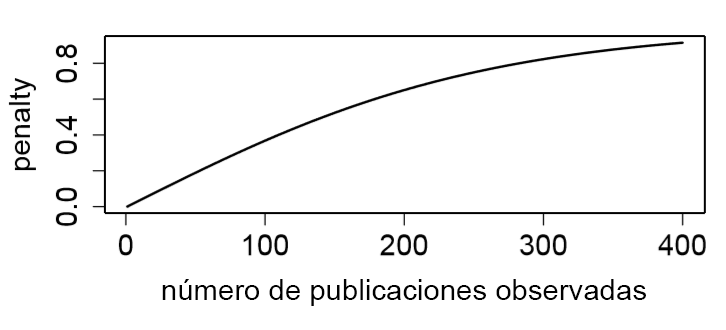
\includegraphics[width=.6\textwidth]{images/penalty}
    \caption{Aumento de la penalización $penalty(k_u)$ en relación al número de publicaciones observadas ($k_u$) antes de tomar la decisión.}
    \label{fig:penalty}
\end{figure}

Más precisamente, la medida $F_{latency}$ se calcula multiplicando la medida $F_1$ tradicional con un valor que representa la velocidad con la que se clasificaron todos los usuarios del conjunto de prueba.
Este último valor se denomina $speed$ y su cálculo se realiza utilizando la mediana de todas las penalizaciones $penalty(k_u)$ obtenida para todos los usuarios, $u$, del conjunto de prueba. En símbolos, siendo $U_{vp}$ el conjunto de usuarios del conjunto de prueba clasificados correctamente como en riesgo (verdaderos positivos), $speed$ se define como:

$$speed = 1 - \text{mediana}\{penalty(k_u) / u \in U_{vp}\}$$
% $$speed = (1 - \text{median}\{penalty(k_u) / u \in U, d_u = g_u = 1\})$$

Y finalmente, $F_{latency}$ se define como:

\begin{equation}
F_{latency} = F_1 \times speed
\label{eq:flatency}
\end{equation}


\


La medida $F_{latency}$ surge como una alternativa a la medida $ERDE_o$ que intenta solucionar algunos defectos de esta última~\cite{sadeque2018measuring}.
Por ejemplo, si bien la medida $ERDE_o$ permite realizar comparaciones relativas entre modelos,\footnote{Ya que por definición se tiene que mientras más rápido y efectivo sea un modelo, más cercano a $0$ será su valor $ERDE_o$, es decir, más cercano a nulo será el error acumulado.} su semántica en término de su valor absoluto no es tan clara.\footnote{¿Qué significa que el valor $ERDE_5$ obtenido haya sido de, por ejemplo, $11.31\%$?¿fue el modelo rápido o lento?}
En su lugar, la medida $F_{latency}$ posee una semántica más clara debido a que su valor se apoya en la medida $F_1$ tradicional, cuya semántica es bien conocida y captura la efectividad de la clasificación, y un valor de penalización que explícitamente captura la demora de la misma.
Además, en la medida $ERDE_o$, la penalización por la demora en la clasificación es virtualmente binaria, es decir, será siempre $0$ para modelos clasificando correctamente a los usuarios antes de procesar $o$ publicaciones, y $1$ para un número mayor de publicaciones. 
En su lugar, la penalización en la medida $F_{latency}$ va aumentando gradualmente conforme se procesen más documentos.
Sin embargo, creemos adecuado no pensar la medida $F_{latency}$ como superior a $ERDE_o$, sino más bien como capturando distintos aspectos de la clasificación anticipada, es decir, al igual que las medidas tradicionales $recall$ y $precision$ no son superiores la una de la otra, sino que ambas capturan distintos aspectos de la clasificación de documentos, $ERDE_o$ y $F_{latency}$ nos brindan información vinculada a distintos aspectos de la clasificación anticipada.
Por ejemplo, debido a que la medida $F_{latency}$ utiliza la medida $F_1$, su utilización resaltará a modelos que le asignen la misma importancia tanto a $recall$ como a $precision$, mientras que la medida $ERDE_o$ resaltará a los modelos que prioricen $recall$ por sobre $precision$,\footnote{Esto se debe a la forma en que se calcula la medida $ERDE_o$ (\autoref{eq:erde}), siendo el costo de los falsos positivos ($cfp$) considerablemente más pequeño que el de los falsos negativos ($cfn$).} lo que no es necesariamente malo teniendo en cuenta que se lidia con tareas de riesgo en donde cada usuario (positivo) no detectado es una vida en riesgo.
De la misma manera, el hecho de que la penalización de la medida $ERDE_o$ sea binaria no necesariamente representa un defecto si se tiene en cuenta la naturaleza binaria de cualquier tarea de riesgo, en donde existe un punto específico en el tiempo que se intenta anticipar y que, pasado el mismo, ya es demasiado tarde para una clasificación efectiva\footnote{Tal vez una mejor manera, más realista, de utilizar la medida $ERDE_o$ podría obtenerse simplemente al asignar, en lugar de un único valor $o$ fijo para todos los usuarios en riesgo, un valor $o$ específico para cada uno de ellos que refleje el punto en el tiempo al que los modelos deben anticiparse específicamente para ese usuario.} ---a diferencia de otras tareas de clasificación anticipada en las que el costo a pagar por una demora aumenta gradualmente con el tiempo.

% Tenga en cuenta que la mayoría de los valores ERDE están relativamente cerca entre sí, esto se debe a la forma en que se calculó $ERDE$.\footnote{$cfp = \frac{\#positive\_users}{\#users}$ por lo tanto cada usuario, clasificado erróneamente como falso positivo, agregó un valor de $\frac{cfp}{\#users} = \frac{\#positive\_users}{\#users^2} = \frac{73}{815^2} = 0.0001$ al final/informado $ERDE$ (y 0.001 en caso de falso negativo o verdadero positivo después del umbral de $o$).} Cuanto más grande y desequilibrado sea el conjunto de datos, asintóticamente más planos y más cercanos son los valores de $ERDE$ (como sucedió con esta tarea). Por lo tanto, los decimales importan mucho cuando se trata de la medida de $ERDE$. Por ejemplo, en esta tarea, solo una pequeña diferencia de 0.009 (0.9\%) en $ERDE$ en realidad significa que el 12\% de todos los usuarios anoréxicos o no anoréxicos no fueron clasificados adecuadamente, lo cual es una diferencia significativa.


% This metric try to overcome some limitations of ERDE, namely:

% – the penalty associated to true positives goes quickly to 1. This is due to the functional form of the cost function (sigmoid).
% – a perfect system, which detects the true positive case right after the first round of messages (first chunk), does not get error equal to 0.
% – with a method based on releasing data in a chunk-based way (as it was done in 2017 and 2018) the contribution of each user to the performance evaluation has a large variance (different for users with few writings per chunk vs users with many writings per chunk).
% – ERDE is not interpretable.

% En su lugar, $F_{latency}$ has the following nice properties:
% – smooth grow of penalties.
% – a perfect system gets Flatency = 1 .
% – for each user $u$ the system can opt to stop at any point ku and, therefore, now we do not have the effect of an imbalanced importance of users. ????
% – Flatency is more interpretable than ERDE.

% Sin embargo, no coincidimos con los autores, 



% Sin embargo, cualquiera de estas dos medidas tiene el problema de ... entonces también se incluyeron medidas basadas en ranking que son independientes de la decisón y se centran en ver que tan bien los modelos creen que cada usuario está en riesgo. (algo así)

% Sin embargo, en lugar de tener un modelo que clasifique los usuarios, se podría tener un modelo que le asigne un ``grado de riesgo'' a cada usuario y luego le presente a los expertos un ranking ordenado en por grado de riesgo para que ellos tomen la decisión. Este ranking iría constantemente cambiando con forme se vayan procesando nuevas publicaciones.

\subsection{Medidas Basadas en Ranking}

En esta edición del eRisk, como complemento de las medidas $ERDE$ y $F_{latency}$, también se utilizaron medidas basadas en ranking.
Por este motivo, luego de que los modelos solicitaran la siguiente publicación de cada usuario al servidor, se les pidió a los modelos que le respondieran al servidor, no sólo con la decisión sobre cada usuario, sino también con una puntuación que represente el grado de riesgo de cada usuario, estimado por el modelo hasta ese momento.
Luego, ordenando todos los usuarios según la puntuación asignada por el modelo, se puede obtener un ranking de usuarios dado por el grado de riesgo estimado. %por cada modelo participante.
Como consecuencia, en cada instante de tiempo es posible obtener un ranking de usuarios asociado a cada modelo participante ---\emph{e.g.} un ranking luego de leer la primer publicación, uno luego de leer la segunda, y así sucesivamente.
De esta manera se busca simular un enfoque de reordenamiento continuo de usuarios en base a la incorporación de nueva evidencia, lo que en una aplicación de la vida real permitiría que el ranking actual pueda ser presentado a expertos humanos, en cualquier momento que sea necesario ---dichos expertos serían luego los encargados de tomar las decisiones correspondientes analizando a los usuarios con mayor grado de riesgo estimado, es decir, los primeros usuarios del ranking.

La evaluación del desempeño de los modelos en este tipo de escenarios se puede llevar a cabo simplemente utilizando las medidas de calidad de ranking tradicionales del campo de la \emph{Recuperación de Información}.
De esta forma, al medir la calidad de los distintos rankings estaremos evaluando el desempeño de los distintos modelos en relación a qué tan bien estiman el grado de riesgo de los usuarios.
En particular, las medidas de calidad de ranking utilizadas en esta edición del eRisk fueron las medidas $P@k$ y $NDCG@k$. Más precisamente, se utilizaron las medidas $P@10$, $NDCG@10$ y $NDCG@100$, las cuales fueron reportadas, por cada modelo, para 4 rankings distintos, respectivamente, el ranking obtenido luego de leer $1$, $100$, $500$ y $1000$ publicaciones.

La medida $P@k$ se denomina como ``Precisión a los $k$'', y corresponde al porcentaje de resultados relevantes presentes entre los $k$ primeros del ranking. En el caso del eRisk, los resultados relevantes se corresponderían a los usuarios que efectivamente están en riesgo, por lo que en esta tarea la medida $P@k$ es el porcentaje de usuarios en riesgo presentes entre los $k$ primeros resultados del ranking.

La medida $NDCG@k$ del inglés ``Normalized Discounted Cumulative Gain'', es la versión normalizada de la medida $DCG@k$, la cual se calcula como:

$$DCG@k = \sum_{i=1}^k \frac{rel_i}{log_2\left(i+1\right)}$$

Donde $rel_{i}$ es el grado de relevancia del resultado presente en la posición $i$ del ranking. En el caso del eRisk, el grado de relevancia es binario, siendo $1$ para los usuarios en riesgo y $0$ para los que no. La idea principal detrás de este medida es penalizar a los resultados relevantes en relación a qué tan abajo en el ranking hayan aparecido.
Finalmente, la normalización se lleva a cabo en relación al $DCG@k$ que obtendría el ranking ideal,\footnote{En el caso de las tareas del eRisk, el ranking ideal sería el ranking en donde todos los usuarios en riesgo se encuentran al comienzo del ranking y luego el resto de usuarios.} denotado por $IDCG@k$, en símbolos:

\begin{equation}
NDCG@k = \frac{DCG@k}{IDCG@k}
\end{equation}


\section{Detalles de Implementación}
\label{sec:erisk2019implementacion}

% La implementación se llevó a cabo de forma análoga a los capítulos anteriores ya que, como se mencionó al inicio, el fin principal de nuestra participación fue el de comprobar si los resultados obtenidos en la práctica eran, efectivamente, consistentes con los obtenidos en los capítulos anteriores, por medio de la experimentación.

Como el objetivo principal es evaluar más en detalle la robustez y el desempeño de los modelos propuestos en los capítulos anteriores sobre un nuevo conjunto de datos, se utilizaron los mismos valores de hiperparámetros que en los capítulos anteriores, es decir $\lambda=\rho=1$ y $\sigma= 0.455$. Como se describió en el \autoref{cap:ss3}, estos valores fueron originalmente seleccionados para optimizar la medida $ERDE_{50}$ en la tarea del eRisk 2017 y luego, como se observó en el \autoref{cap:tss3}, también mostraron ser robustos en las tareas del eRisk 2017 y 2018, en donde tanto SS3 como $\tau$-SS3 se desempeñaron consistentemente bien en términos de la medida $ERDE$.
Por el mismo motivo, se utilizó nuevamente la suma de vectores como el \emph{operador de resumen} ($\oplus_j$) para todo nivel $j$ y la misma política de clasificación anticipada que en el capítulo anterior ---es decir, los usuarios se clasificaron como positivo tan pronto como el \emph{valor de confianza} positivo, acumulado hasta ese momento, fuese mayor que el negativo.
% Finalmente, con respecto al preprocesamiento, no se utilizó ningún método especial salvo una simple normalización eliminando los acentos y convirtiendo el texto a minúsculas, al igual que en el capítulo anterior.\footnote{
% Se probaron otros métodos como \emph{stemming} y \emph{lemmatization} utilizando el paquete \emph{Natural Language Toolkit} (NLTK) de Python, pero al contrario de lo que esperábamos inicialmente, el rendimiento del modelo se redujo.}

\begin{figure}[t]
    \begin{subfigure}{0.5\textwidth}
        \centering
        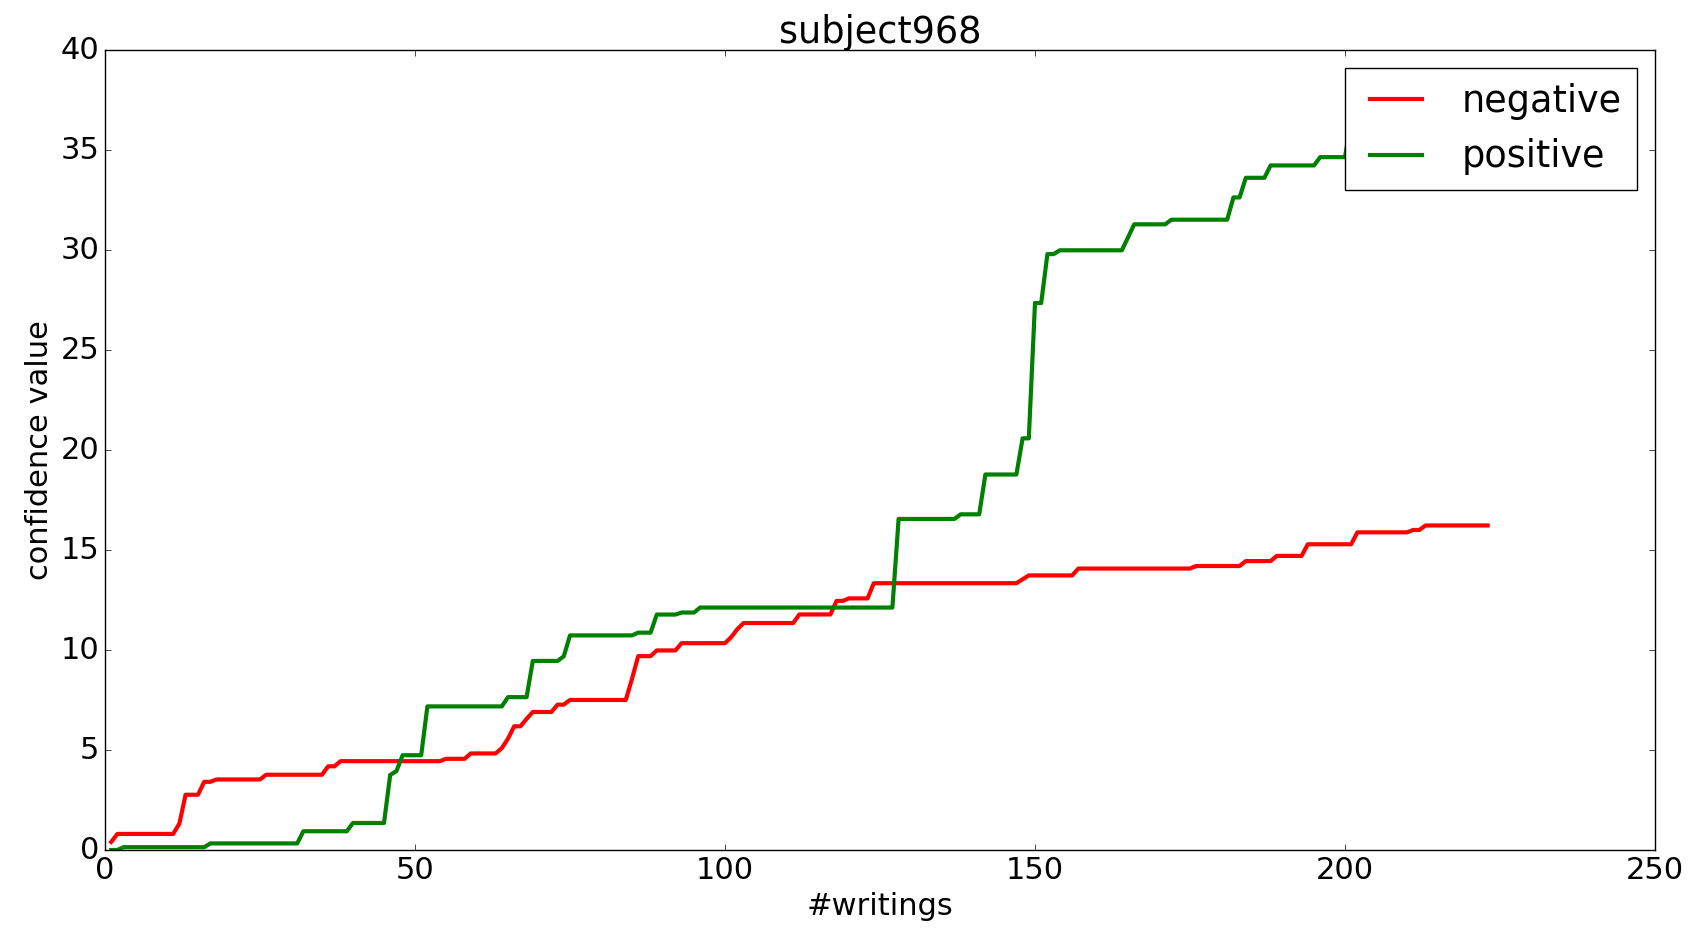
\includegraphics[width=80mm]{images/subject968}
        \caption{}
    \end{subfigure}
    \begin{subfigure}{0.5\textwidth}
        \centering
        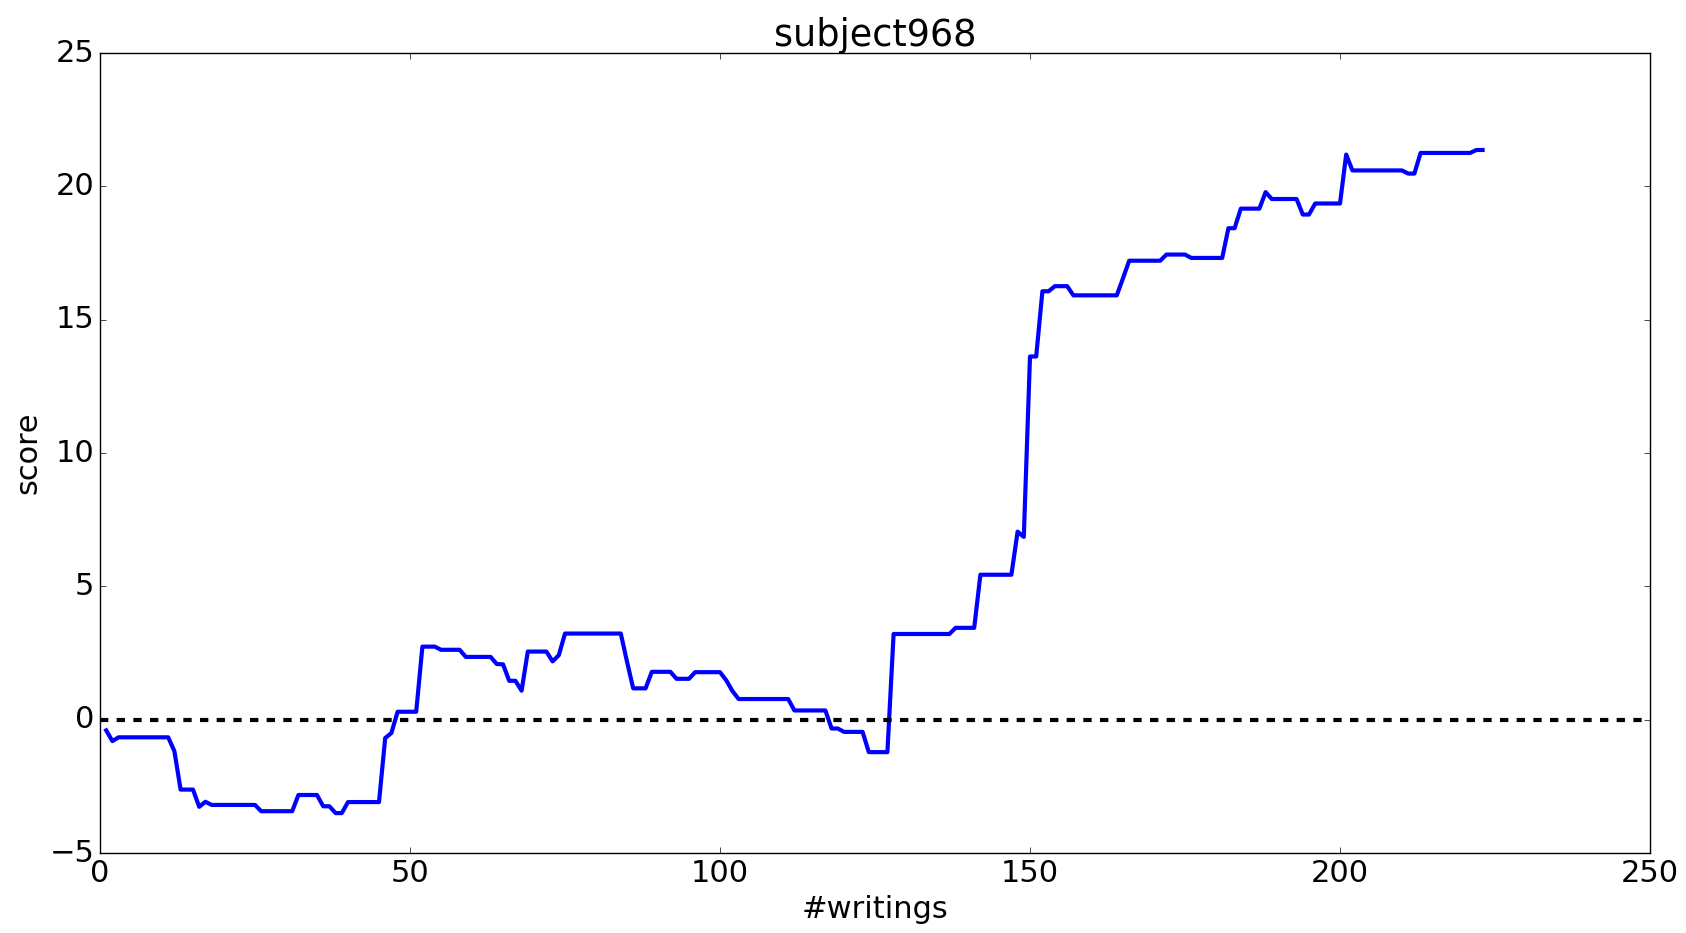
\includegraphics[width=80mm]{images/subject968-score}
        \caption{}
    \end{subfigure}
\caption{
    Sujeto 968 del conjunto de prueba para la tarea de detección anticipada de anorexia.
    (a) Variación del \emph{valor de confianza} positivo y negativo a lo largo del tiempo, publicación a publicación.
    (b) Variación de la \emph{puntuación} estimada ($positivo-negativo$) a lo largo del tiempo, publicación a publicación.
}
\label{fig:subject968}
\end{figure}

% \begin{figure}[t!] % [t]op; [h]ere; [p]age; [b]ottom; [r]ight; [l]eft
%     \centering
%     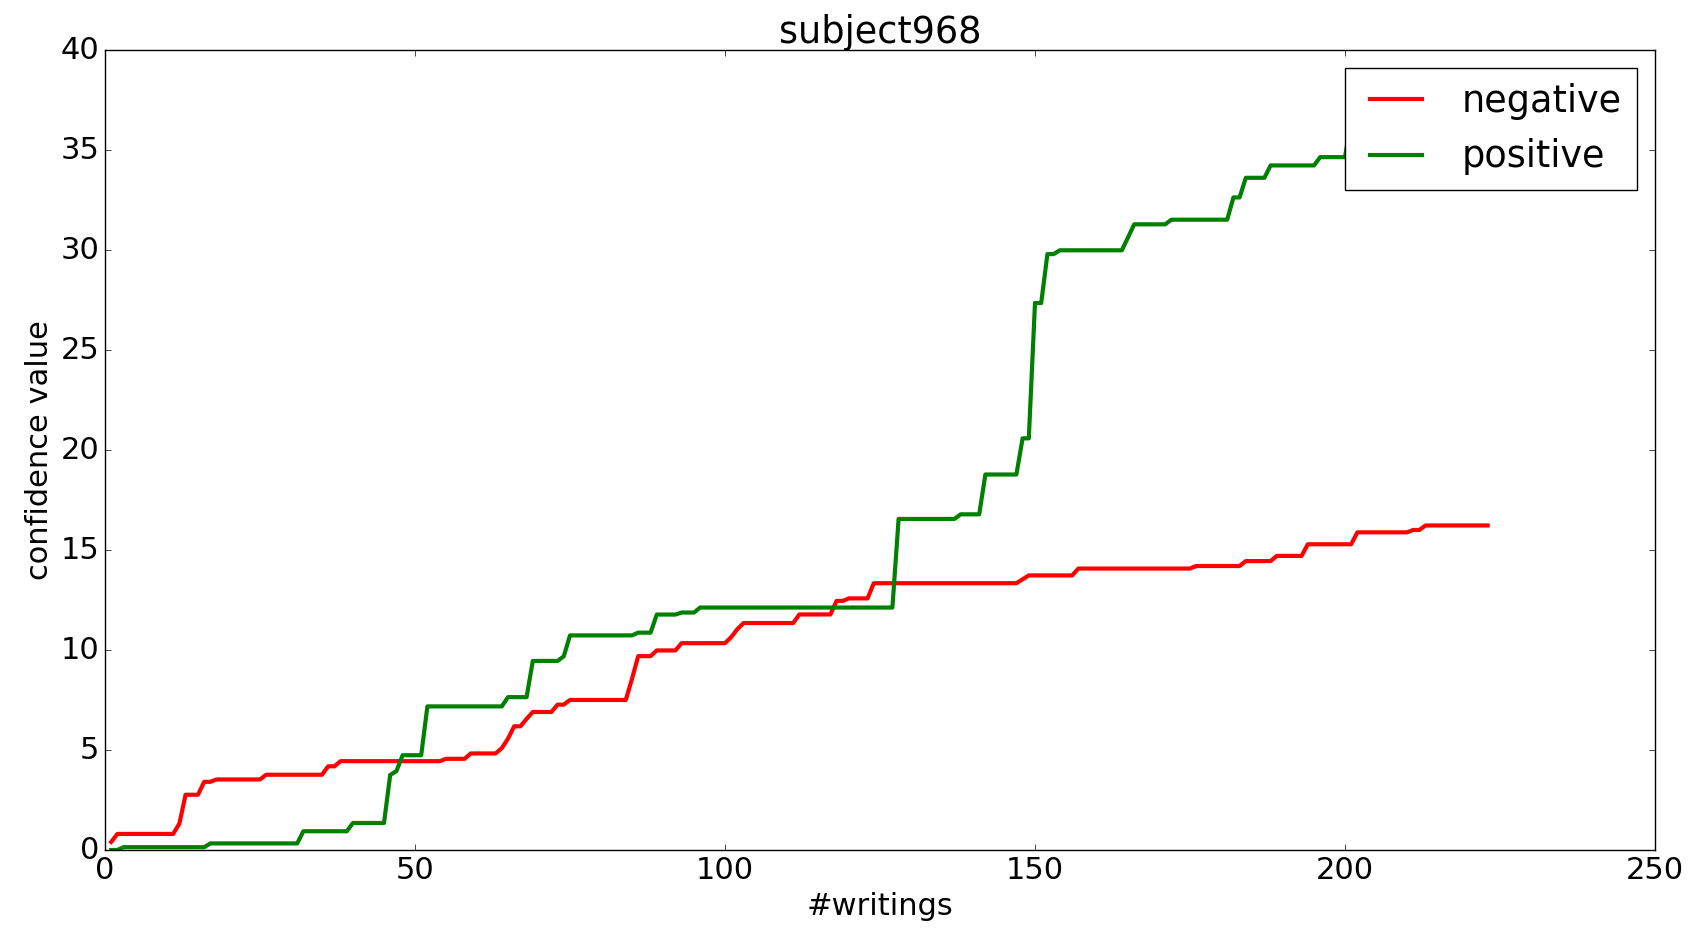
\includegraphics[width=120mm]{images/subject968}
%     \caption{Variación del valor de confianza positivo y negativo del sujeto 968 a lo largo del tiempo (publicaciones).}%Task 3's subject 968's positive and negative confidence value variation over time (writings).
%     \label{fig:subject2341}
% \end{figure}

% \begin{figure}[t!] % [t]op; [h]ere; [p]age; [b]ottom; [r]ight; [l]eft
%     \centering
%     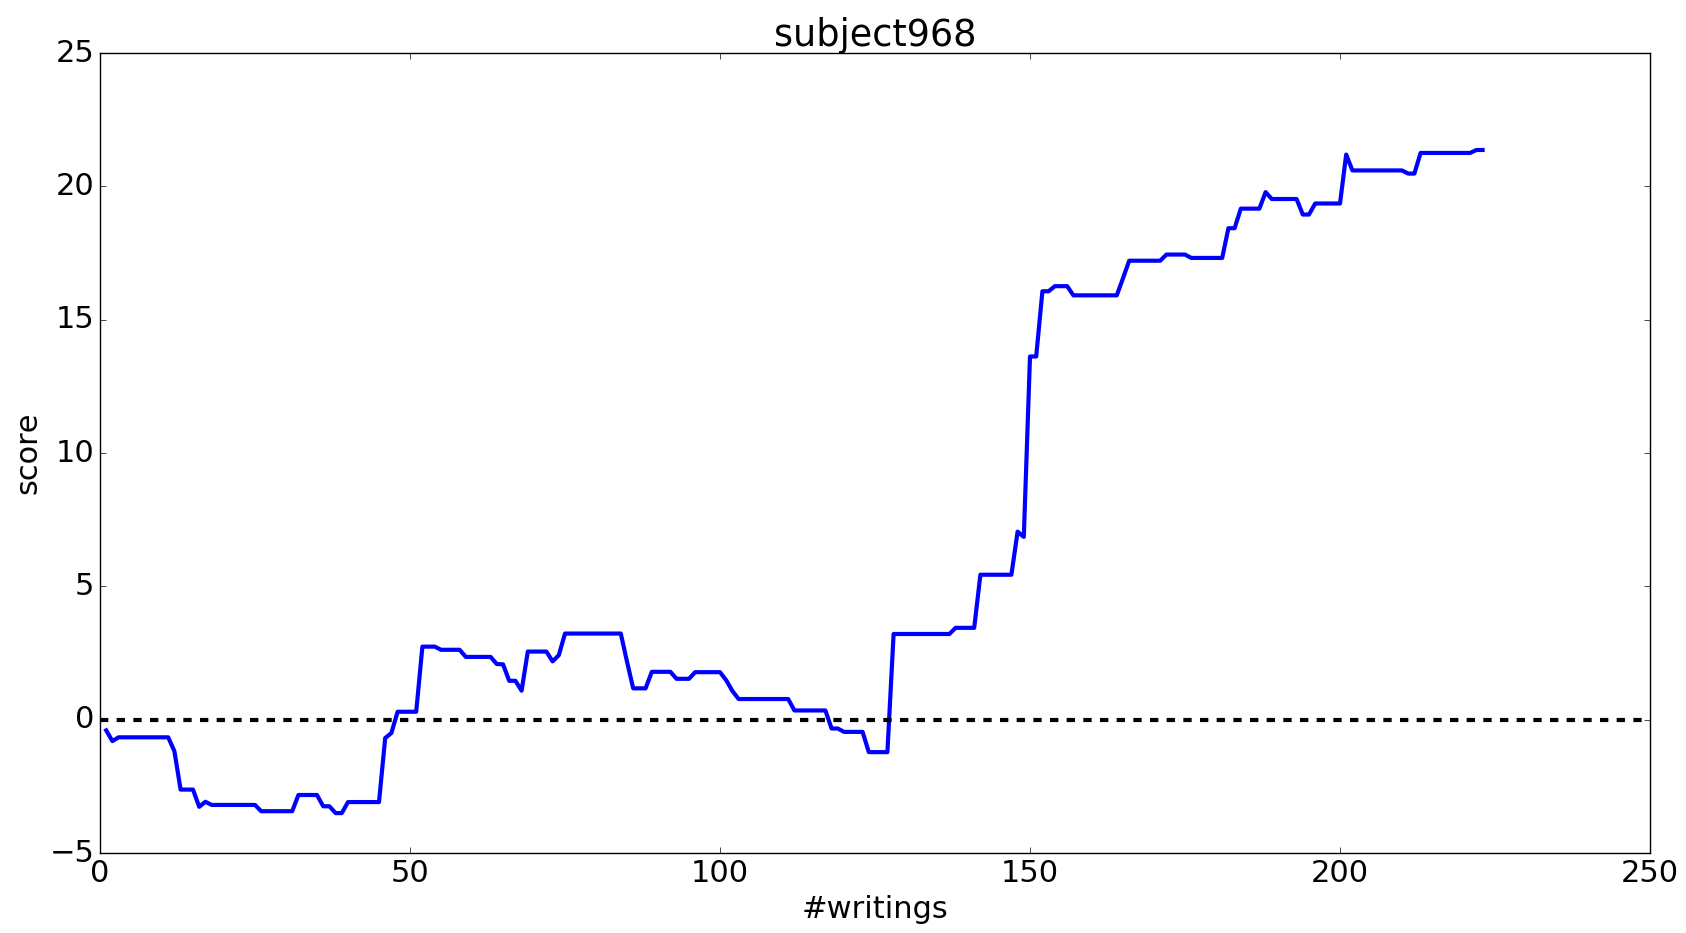
\includegraphics[width=120mm]{images/subject968-score}
%     \caption{Puntuación estimada del nivel de anorexia ($positivo-negativo$) de la tarea 1 del sujeto 968 a lo largo del tiempo (escritos).}%Task 1's subject 968's estimated score of the level of anorexia ($d[positive]-d[negative]$) variation over time (writings).
%     \label{fig:subject2341-cv}
% \end{figure}

% %where $WH_s$ is the subject's writing history. Note that for all the tasks $\overrightarrow{d_s}$ was a vector with two components, one for the positive class and the other for the negative one. The policy to classify a subject as positive was performed analyzing how $\overrightarrow{d_s}$ changed over time, as shown with an example in \autoref{fig:subject2341}. Subjects were classified as positive when the positive value in $\overrightarrow{d_s}$ exceeded the negative one\footnote{Except for task T3 in which we did not perform an "early stop", and therefore every user was classified after processing the entire writing history.}, for instance, the subject in the figure was classified as anorexic after reading the 42nd writing.
% aquí $WH_s$ es la historia de escritura del sujeto. Tenga en cuenta que para todas las tareas $\overrightarrow{d_s}$ era un vector con dos componentes, uno para la clase positiva y el otro para la negativa. La política para clasificar un sujeto como positivo se realizó analizando cómo $\overrightarrow{d_s}$ cambió con el tiempo, como se muestra con un ejemplo en \autoref{fig:subject2341}. Los sujetos fueron clasificados como positivos cuando el valor positivo en $\overrightarrow{d_s}$ excedió al negativo\footnote{Excepto para la tarea T3 en la que no realizamos una "parada temprana", y por lo tanto cada usuario fue clasificado luego de procesar todo el historial de escritura.}, por ejemplo, el sujeto de la figura fue clasificado como anoréxico después de leer el 42º escrito.

%Finally, this year, models performance were also evaluated based on ranking-based measures for tasks T1 and T2. Thus, models were asked to provide an estimated score of the level of anorexia/self-harm along with the binary decision (0/1). To compute this score, SS3 performed the difference between the positive confidence value and the negative one (i.e. $d[positive]-d[negative]$) and returned it along with each decision. For example, in \autoref{fig:subject2341-cv} is shown how this score changed as more writings were read, for the same user shown previously in \autoref{fig:subject2341}.
Como se describió en la sección anterior, en esta edición del eRisk se les pidió a los modelos que, junto con la decisión, proporcionaran una puntuación del nivel de riesgo estimado de cada usuario ---utilizado luego para generar los rankings.
Dicha puntuación fue calculada simplemente considerando la diferencia entre el \emph{valor de confianza} positivo y el negativo, esto es:

\begin{equation}
\text{\emph{puntuación}} = \text{\emph{valor de confianza positivo}} - \text{\emph{valor de confianza negativo}}
\label{eq:puntuacion}
\end{equation}


Como se ilustra con un ejemplo en la \autoref{fig:subject968}, esta simple diferencia permite que, en todo momento, los dos valores de confianza positivo y negativo puedan ser representados por un único valor de confianza unificado, el cual ya no representa el valor de confianza de cada clase, sino más bien un valor de confianza de ``toma de decisión'' que representaría, efectivamente, el nivel de riesgo estimado por el modelo ---ya que es el valor utilizado por el modelo para, efectivamente, clasificar y detectar a los usuarios en riesgo.


\section{Tareas y Resultados Obtenidos}

Esta sección describe la participación en el eRisk 2019 con los modelos propuestos en los capítulos anteriores. En las siguientes secciones se describe cada tarea  y se examinan los resultados obtenidos en cada una de las mismas.


\subsection{Tarea 1: Detección Anticipada de Anorexia}%Task 1: Early Detection of Signs of Anorexia

\begin{table*}[t]
\centering
\caption{Estadísticas principales del conjunto de datos de la tarea 1.}
\label{tab:dataset-t1}
\begin{tabular}{l c c|c c}
\hline
& \multicolumn{2}{c}{Entrenamiento} & \multicolumn{2}{c}{Prueba}\\
& Anorexia & Control & Anorexia & Control \\ \hline
No. de sujetos & 61 & 411 & 73 & 742 \\
No. de publicaciones & 24874 & 228878 & 17619 & 552890 \\
Prom. de publicaciones por sujeto & 407.8 & 556.9 & 241.4 & 745.1 \\
Prom. de días (primera a última publ.) & 800 & 650 & 510 & 930 \\
Prom. de palabras por publicación & 37.3 & 20.9 & 37.2 & 21.7 \\ \hline

\hline
\end{tabular}
\end{table*}


En esta tarea participaron un total de 13 equipos de investigación distintos y se enviaron un total de 50 modelos distintos.
Como se describe más detalladamente en la descripción general del eRisk~\cite{losadaetal2019}, esta tarea se planteó como una continuación de la tarea de detección anticipada de anorexia del eRisk 2018, por lo que, en esta nueva edición, el conjunto de entrenamiento se conformó uniendo el conjunto de entrenamiento y el de prueba de esa edición.
La evaluación de los modelos se llevó a cabo utilizando un nuevo conjunto de prueba construido con la misma metodología que en las ediciones anteriores, es decir, recolectando las publicaciones de un conjunto de usuarios de Reddit divididos en dos grupos, aquellos diagnosticados con anorexia y aquellos que no.
En la \autoref{tab:dataset-t1} se brindan las principales estadísticas del conjunto de datos completo, en donde se puede observar que, nuevamente, las clases están altamente desbalanceadas ---por ejemplo, sólo $73$ de los $815$ usuarios del conjunto de prueba están etiquetados como en riesgo.


\

La participación en esta tarea se llevó a cabo utilizando $5$ modelos distintos, los cuales fueron nombrados dentro del eRisk respectivamente como \emph{UNSL\#0, UNSL\#1, UNSL\#2, UNSL\#3, UNSL\#4}.\footnote{Los nombres de los modelos participantes fueron conformados por el nombre registrado para su equipo, en nuestro caso ``UNSL'', seguido de un \# y su respectivo número.} 
Como se detalló en la \autoref{sec:erisk2019implementacion}, se utilizaron los mismos valores de hiperparámetros para los $5$ modelos. Por lo tanto, la principal diferencia entre cada uno de estos modelos estuvo dada por la manera en la que fueron entrenados y el tipo específico de modelo SS3 utilizado, como se detalla a continuación:

\begin{itemize}
\item \emph{UNSL\#0}: modelo SS3 original entrenado con el conjunto de entrenamiento del eRisk 2018, excluyéndose así del entrenamiento a los usuarios correspondientes al conjunto de prueba de esa misma edición.
De esta manera, el modelo obtenido se correspondió al utilizado en el capítulo anterior, permitiendo evaluar la consistencia y robustez de los resultados en relación a los obtenidos previamente en la experimentación controlada.
\item \emph{UNSL\#1}: análogo al modelo anterior pero utilizando $\tau$-SS3 en lugar de SS3.
% este modelo es el mismo que el anterior pero permitiendo que SS3 reconozca bigramas de palabras.
\item \emph{UNSL\#2}: modelo SS3 entrenado utilizando el conjunto de entrenamiento completo disponible para esta edición. Esto es, el modelo se entrenó utilizando tanto los usuarios del conjunto del entrenamiento como los de prueba del eRisk 2018.
\item \emph{UNSL\#3}: análogo al modelo anterior pero utilizando $\tau$-SS3 en lugar de SS3.
\item \emph{UNSL\#4}: modelo UNSL\#2 modificado para que, durante el proceso de clasificación, sólo se tengan en cuenta las palabras con un \emph{valor global} mayor a $0.3$ ---\emph{i.e.} SS3 asignó $gv(w, c_i) = 0$ a todo $w$ y $c_i$ tal que $gv(w, c_i)\leq0.3$.\footnote{Utilizando los datos del conjunto de entrenamiento se probaron, comenzando en $0$, incrementalmente distintos valores, eligiéndose así $0.3$ por haber obtenido el mejor valor $ERDE_{50}$.}
Con esta variante se intentó medir qué impacto tienen las palabras con bajo \emph{valor global} en el desempeño de clasificación, es decir, con este modelo se buscó abordar preguntas tales como: ``¿qué tan sensible es el modelo al ruido que podrían introducir la gran cantidad de palabras con un \emph{valor global} bajo?'' o ``¿podría ser el caso de que a causa de estas palabras la condición de clasificación anticipada se dispare incorrectamente producto del ruido acumulado al procesarlas?''.
% Este modelo obtuvo el mejor valor $ERDE_{50}$.
% con esta variante se buscó evitar que el modelo sea demasiado sensible al ruido que podrían introducir palabras con un \emph{valor global} bajo.
% La hipótesis fue que estas palabras con bajo \emph{valor global} podrían causar que la condición de clasificación anticipada se dispare incorrectamente producto del ruido acumulado al procesarlas.
\end{itemize}


\vspace{5mm}

A continuación se presentarán los resultados obtenidos para esta tarea,
sin embargo, es adecuado mencionar previamente que a ninguno de los participantes se le permitió optimizar sus modelos en relación a las nuevas medidas, ya que las mismas sólo se dieron a conocer junto con la publicación de los resultados finales.
Así, los principales resultados obtenidos con los 5 modelos descritos anteriormente, agrupados según las medidas utilizadas para medir el desempeño de los mismos, son los siguientes:
% Estos resultados son presentados en tres grupos distintos dependiendo del desempeño medido, uno para las medidas centradas en la decisión,  como las basadas en ranking, se podrían resumir de la siguiente manera:

% Los principales resultados globales obtenidos en esta tarea, tanto para las medidas centradas en la decisión como las basadas en ranking, se podrían resumir de la siguiente manera:

\begin{table*}[t!]
\centering
\caption{Resultados obtenidos en la tarea 1 para las medidas centradas en la decisión. A modo de comparación, del total de 50 modelos participantes, aquí se muestran, ordenados por $ERDE_{50}$, sólo los modelos que obtuvieron los mejores valores de cada uno de los otros 12 equipos de investigación.}
\label{tab:t1-result}
\begin{tabular}{l c c c c c c c c c c}
\hline
% Team\#run & P & R & $F1$ & $F2$ & $ERDE_5$ & $ERDE_{50}$ & $F_{latency}$ & $F2_{latency}$ \\
Equipo\#modelo & $ERDE_5$ & $ERDE_{50}$ & $F_{latency}$\\ \hline

UNSL\#0 & \textbf{5.53\%} & 3.92\% & .55 \\
UNSL\#1 & 5.68\% & 4.10\% & .55 \\
UNSL\#2 & 5.56\% & 3.34\% & .50 \\
UNSL\#3 & 5.59\% & 3.48\% & .49 \\
UNSL\#4 & 6.14\% & \textbf{2.96\%} & .46 \\
\hline
\hline
CLaC\#1 & 5.73\% & 3.13\% & \textbf{.69} \\
BiTeM\#1 & 5.89\% & 3.40\% & .54 \\
CLaC\#4 & 6.25\% & 3.42\% & \textbf{.69} \\
UDE\#0 & 8.48\% & 3.87\% & .58 \\
UDE\#1 & 7.48\% & 3.94\% & .53 \\
INAOE-CIMAT\#0 & 9.29\% & 3.98\% & .62 \\
LTL-INAOE\#1 & 7.74\% & 4.20\% & .55 \\
INAOE-CIMAT\#3 & 9.17\% & 4.75\% & .63 \\
SINAI\#2 & 9.04\% & 4.89\% & .30 \\
INAOE-CIMAT\#4 & 9.12\% & 5.07\% & .61 \\
lirmm\#0 & 9.13\% & 5.14\% & .63 \\
UppsalaNLP\#4 & 5.73\% & 5.66\% & .41 \\
BioInfo@UAVR\#0 & 5.84\% & 5.77\% & .37 \\
lirmm\#3 & 9.08\% & 6.62\% & .48 \\
SSN-NLP\#3 & 7.61\% & 6.86\% & .33 \\
HULAT\#0 & 10.84\% & 8.14\% & .16 \\
UDE\#2 & 12.52\% & 8.21\% & .53 \\
Fazl\#2 & 17.11\% & 11.22\% & .14 \\
Fazl\#1 & 17.11\% & 13.91\% & .11 \\

\hline
\end{tabular}
\end{table*}

% \begin{table*}[t!]
% \centering
% \caption{Resultados de la Tarea 1, evaluación basada en decisiones. Los mejores resultados de cada uno de los 13 equipos también se muestran para comparar.}%Results for Task 1, decision-based evaluation. Best results are also shown for comparison.
% \label{tab:t1-result}
% \begin{tabular}{l c c c c c c c c c c}
% \hline
% % Team\#run & P & R & $F1$ & $F2$ & $ERDE_5$ & $ERDE_{50}$ & $F_{latency}$ & $F2_{latency}$ \\
% Team\#run & P & R & $F1$ & $ERDE_5$ & $ERDE_{50}$ & $F_{latency}$ & $F2_{latency}$ \\ \hline

% % BiTeM\#1 & .44 & .70 & .54 &  & .06 & .03 & .54 \\
% UDE\#0 & .51 & .74 & .61 & 8.48\% & 3.87\% & .58 & .64 \\
% lirmm\#1 & \textbf{.77} & .60 & .68 & 9.09\% & 5.50\% & .62 & .57 \\
% lirmm\#2 & .66 & .70 & .68 & 9.24\% & 5.80\% & .60 & .60 \\
% Fazl\#2 & .09 & \textbf{1} & .16 & 17.11\% & 11.22\% & .14 & .28 \\
% CLaC\#0 & .45 & .74 & .56 & 6.72\% & 3.93\% & .54 & .63 \\
% CLaC\#1 & .61 & .82 & .70 & 5.73\% & 3.12\% & .69 & \textbf{.75} \\
% CLaC\#2 & .60 & .81 & .69 & 6.01\% & 3.13\% & .68 & .73 \\
% CLaC\#3 & .63 & .81 & .69 & 6.27\% & 3.54\% & .68 & .74 \\
% CLaC\#4 & .64 & .79 & \textbf{.71} & 6.25\% & 3.42\% & \textbf{.69} & .73 \\
% LTL-INAOE\#1 & .47 & .75 & .58 & 7.74\% & 4.19\% & .55 & .64 \\
% INAOE-CIMAT\#0 & .56 & .78 & .66 & 9.29\% & 3.98\% & .62 & .68 \\
% INAOE-CIMAT\#3 & .67 & .68 & .68 & 9.17\% & 4.75\% & .63 & .69 \\
% INAOE-CIMAT\#4 & .69 & .63 & .66 & 9.12\% & 5.07\% & .61 & .59 \\
% UNSL\#0 & .42 & .78 & .55 & \textbf{5.53\%} & 3.92\% & .55 & .66 \\
% UNSL\#1 & .43 & .75 & .55 & 5.68\% & 4.10\% & .55 & .65 \\
% UNSL\#2 & .36 & .86 & .51 & 5.56\% & 3.34\% & .50 & .67 \\
% UNSL\#3 & .35 & .85 & .50 & 5.59\% & 3.48\% & .49 & .66 \\
% UNSL\#4 & .31 & .92 & .47 & 6.14\% & \textbf{2.96\%} & .46 & .65 \\

% % UDE\#0 & .51 & .74 & .61 & .67 & .08 & .04 & .58 & .64 \\
% % lirmm\#1 & \textbf{.77} & .60 & .68 & .62 & 9.xx\% & 6.xx\% & .62 & .57 \\
% % lirmm\#2 & .66 & .70 & .68 & 69 & .09 & .06 & .60 & .60 \\
% % Fazl\#2 & .09 & \textbf{1} & .16 & .33 & 17.xx\% & 11.xx\% & .14 & .28 \\
% % CLaC\#0 & .45 & .74 & .56 & .65 & .07 & .04 & .54 & .63 \\
% % CLaC\#1 & .61 & .82 & .70 & .76 & .06 & .03 & .69 & .75 \\
% % CLaC\#2 & .60 & .81 & .69 & .75 & .06 & .03 & .68 & .73 \\
% % CLaC\#3 & .63 & .81 & .69 & .76 & .06 & .03 & .68 & .74 \\
% % CLaC\#4 & .64 & .79 & \textbf{.71} & .75 & 6.xx\% & 3.xx\% & \textbf{.69} & .73 \\
% % LTL-INAOE\#1 & .47 & .75 & .58 & .67 & .08 & .04 & .55 & .64 \\
% % INAOE-CIMAT\#0 & .56 & .78 & .66 & .72 & .09 & .04 & .62 & .68 \\
% % INAOE-CIMAT\#3 & .67 & .68 & .68 & .75 & .09 & .05 & .63 & .69 \\
% % INAOE-CIMAT\#4 & .69 & .63 & .66 & .64 & .09 & .05 & .61 & .59 \\
% % UNSL\#0 & .42 & .78 & .55 & .66 & \textbf{6.xx\%} & 4.xx\% & .55 & .66 \\
% % UNSL\#1 & .43 & .75 & .55 & .65 & 6.xx\% & 4.xx\% & .55 & .65 \\
% % UNSL\#2 & .36 & .86 & .51 & .67 & 6.xx\% & 3.xx\% & .50 & .67 \\
% % UNSL\#3 & .35 & .85 & .50 & .66 & 6.xx\% & 3.xx\% & .49 & .66 \\
% % UNSL\#4 & .31 & .92 & .47 & .66 & 6.xx\% & \textbf{3.xx\%} & .46 & .65 \\

% \hline
% \end{tabular}
% \end{table*}

\begin{itemize}
% UNSL0  ---en relación a los siguientes modelos, éste obtuvo los mejores valores $ERDE_5$ y $F_{latency}$
    \item \textbf{Desempeño centrado en la decisión:} en la \autoref{tab:t1-result} se muestran los resultados obtenidos para las medidas centradas en la decisión.
    En relación a las medidas $ERDE$, se puede observar que el modelo \emph{UNSL\#0} obtuvo el mejor $ERDE_5$ y el \emph{UNSL\#4} el mejor $ERDE_{50}$, no obstante, este último fue el que obtuvo el peor valor $F_{latency}$ de entre los 5 modelos.
    Esto último sugiere que ignorar las palabras con bajo \emph{valor global} puede, de hecho, contribuir a mejorar el desempeño en términos de la medida $ERDE$ pero a costa de un peor desempeño en términos de la medida $F_{latency}$ ya que, en relación al original, el modelo resultante prioriza aún más $recall$ por sobre $precision$,\footnote{\emph{UNSL}\#4 obtuvo el mejor $recall$ ($0.92$) pero el valor $precision$ más bajo ($0.31$).} lo que finalmente afecta la media armónica de estas últimas.
    Los modelos \emph{UNSL\#2} y \emph{\#3} entrenados con el conjunto de entrenamiento completo obtuvieron un mejor desempeño en términos de la medida $ERDE_{50}$ en relación a sus dos contrapartes, \emph{UNSL\#0} y \emph{\#1}, entrenadas sólo con el conjunto de entrenamiento correspondiente a la edición anterior del eRisk ---e.d. los mismos modelos utilizados en el capítulo anterior.
    Sin embargo, el desempeño de estos modelos en términos de la nueva medida $F_{latency}$ fue menor en relación al de estos últimos, esto probablemente se deba a que los hiperparámetros utilizados ajustan el modelo al conjunto de datos en relación a la medida $ERDE_{50}$ ---nuevamente priorizando el $recall$ por sobre su media armónica con la medida $precision$.
    A diferencia de los resultados obtenidos en el capítulo anterior, ambos modelos $\tau$-SS3 (\emph{UNSL\#1 y \#3}) obtuvieron un desempeño ligeramente menor a sus contrapartes utilizando SS3 (respectivamente, \emph{UNSL\#0 y \#2}) con este conjunto de datos.
    Esto tal vez se deba a que el uso de \emph{n-gramas} si bien puede tener cualidades semánticas superiores con respecto a la bolsa de palabras, también sufre de cualidades estadísticas inferiores\footnote{La probabilidad con la que aparece una secuencia de palabras nunca será mayor que la probabilidad individual de cada palabra.} lo que, dependiendo del conjunto de datos utilizado, puede afectar negativamente al desempeño.
    Además, a diferencia del capítulo anterior, aquí los usuarios fueron procesados publicación a publicación y no utilizando los \emph{bloques} de publicaciones ---en donde hasta incluso el modelo más apresurado debió procesar al menos un bloque completo antes de poder tomar una decisión.
    En relación a la nueva medida $F_{latency}$, ninguno de los 5 modelos obtuvo un resultado destacable ya que el mejor valor obtenido ($0.55$), correspondiente a \emph{UNSL\#0} y \emph{\#1}, estuvo $0.13$ puntos por debajo del mejor valor, obtenido por \emph{CLaC\#4} ---del cual se hablará en el siguiente apartado.
    Este resultado se debe principalmente a que, como se mencionó, los 5 modelos utilizaron los mismos valores de hiperparámetros utilizados en los capítulos anteriores, los cuales fueron seleccionados optimizando la medida $ERDE$.
    Por lo tanto, como se explicó al final de la \autoref{sec:medidas_decision}, los modelos resultantes priorizaron tanto el $recall$ como la velocidad.\footnote{En promedio, los 5 modelos SS3 clasificaron a los usuarios en riesgo luego de procesar solamente la segunda o tercera publicación de cada uno de ellos.}
    No obstante, el mejor valor $F_{latency}$ obtenido ($0.55$) se encuentra considerablemente por encima del promedio ($0.38$), ubicándose en el puesto 11 de entre los 50 modelos participantes.
\begin{table*}[t!]
\centering
%\caption{Participating teams for Task 1: number of runs, number of user writings processed by the team, and the time taken for the whole process and for processing each writing (i.e $\frac{TotalTime}{\#writings\times\#runs}$). (*) This value was originally 5, but we replaced it by the actual number of models used.}
\caption{Detalle de los equipos participantes en la tarea 1: nombre del equipo, cantidad de modelos empleados ($\#modelos$), número de publicaciones procesadas de los usuarios ($\#publicaciones$), tiempo total empleado para completar la tarea y tiempo empleado para procesar cada publicación (\emph{i.e.} $\frac{tiempo\ total}{\#publicaciones\times\#modelos}$).}
\label{tab:t1-time}
\begin{tabular}{l c c|c | c}
\hline
& & & \multicolumn{2}{c}{Tiempo} \\
Equipo & \#modelos & \#publicaciones & total & por publicación  \\ \hline

\textbf{UNSL}$\star$ & 5 & 2000 & 23h & \textbf{8s} \\
UppsalaNLP & 5 & 2000 & 2 días + 7h & 20s \\
BioInfo@UAVR & 1 & 2000 & 14h & 25s \\
UDE & 3 & 2000 & 5 días + 3h & 1m + 12s \\
lirmm & 5 & 2024 & 8 días + 15h & 1m + 12s \\
INAOE-CIMAT & 4 & 2000 & 8 días + 2h & 1m + 30s \\
HULAT & 5 & 83 & 18h & 2m + 36s \\
Fazl & 3 & 2001 & 21 días + 15h & 5m + 12s \\
BiTeM & 4 & 11 & 4h & 5m + 30s \\
LTL-INAOE & 2 & 2001 & 17 días + 23h & 6m + 30s \\
SINAI & 3 & 317 & 10 días + 7h & 15m + 36s \\
CLaC & 5 & 109 & 11 días + 16h & 31m \\
SSN-NLP & 5 & 9 & 6 días + 22h & 3h + 42m \\

\hline
\end{tabular}
\end{table*}

    \item \textbf{Desempeño en relación al tiempo de ejecución:} en la \autoref{tab:t1-time} se muestran, por cada equipo, detalles sobre el tiempo total empleado para completar la tarea.
    Como se puede observar, el tiempo tomado para completar la tarea difiere ampliamente de equipo en equipo, variando desde unas pocas hasta una gran cantidad de horas ---en un caso incluso llegando hasta cerca de un mes.
    Sin embargo, para tener una visión más precisa de qué tan eficientes fueron los modelos de cada equipo, no sólo se debe tener en cuenta el tiempo total empleado para completar la tarea sino también la cantidad de publicaciones procesadas en ese tiempo, y el número de modelos utilizados para llevarlo a cabo.
    Por ejemplo, en términos de velocidad de procesamiento, no sería igual de eficiente BiTeM que UNSL, ya que si bien el primero completó la tarea en 4 horas, sólo procesó las primeras 11 publicaciones de cada usuario, mientras que el segundo, si bien demoró 23 horas, procesó la totalidad de las 2000 publicaciones disponibles para cada uno de ellos.
    De la misma manera, no sería igual de eficiente BioInfo@UAVR que UNSL, ya que si bien el primero demoró 14 horas en clasificar a todos los usuarios con un único modelo, el segundo lo tuvo que realizar con 5 de ellos, lo que implicó no sólo un procesamiento 5 veces mayor sino también el envío de 5 veces más peticiones hacia el servidor.\footnote{Por cada una de las 2000 publicaciones no sólo se necesitó una petición para obtener la publicación, sino también se necesitaron 5 peticiones para enviar la respuesta de cada uno de los 5 modelo. Por lo tanto, para grupos como UNSL, completar la tarea requirió de un total de $2000 + 2000*5 = 12000$ peticiones al servidor. Por lo tanto, si la latencia de conexión fue de, por ejemplo, 3 segundos, se tiene que aproximadamente 10 horas del total fueron consumidos sólo en la comunicación.}
    Por este motivo, en la \autoref{tab:t1-time} también se incluye una estimación del tiempo que le tomó a los modelos procesar cada publicación, el cual se obtuvo normalizando el tiempo total en relación a la cantidad de modelos utilizados y el número de publicaciones procesadas por cada uno de ellos.
    Así, se puede observar que UNSL fue el equipo más eficiente en términos de tiempos de ejecución, habiendo procesado cada publicación en aproximadamente 8 segundos\footnote{Ya que este tiempo incluye la latencia de recibir la publicación, el tiempo utilizado efectivamente para procesarla, y luego la latencia del envío de la respuesta, gran parte de estos 8 segundos se corresponden a dichas latencias.} ---\emph{i.e.} 2000 publicaciones de cada usuario procesadas con 5 modelos en 23 horas.
    Vale la pena mencionar que el hecho de que UNSL haya sido el más rápido en procesar cada publicación no se debió a la utilización de un poder de cómputo superior al del resto de los participantes para ejecutar sus modelos,\footnote{Para ejecutar el script Python con los modelos se utilizó la computadora portátil personal del autor del presente documento, la cual tiene especificaciones técnicas ordinarias, por ejemplo, un procesador Intel Core i5 y 8GB de RAM.} sino a la utilización del modelo SS3 que, como vimos en el \autoref{cap:ss3}, fue diseñado para poder trabajar incrementalmente, permitiéndole procesar la secuencia (de publicaciones) de entrada en tiempo de orden $O(n)$, con respecto al largo de la misma.
    Esto contrasta con otros equipos, tales como CLaC~\cite{mohammadi2019quick}, INAOE-CIMAT~\cite{aragon2019inaoe} o lirmm~\cite{ragheb2019attentive}, que si bien obtuvieron un mejor desempeño en relación a, por ejemplo, la medida $F_{latency}$, fueron considerablemente más lentos, tomándole días completar la misma tarea.
    Por ejemplo, los 5 modelos de CLaC~\cite{mohammadi2019quick} emplearon un clasificador \ac{SVM} que tomaba como entrada una representación vectorial obtenida ensamblando varios modelos neuronales basados en mecanismos de atención, uno de los cuales (\emph{CLaC\#1}) obtuvo el mejor valor $F_{latency}$.
    Sin embargo, estos modelos fueron 232 veces más lentos que los modelos SS3 de UNSL, ya que a CLaC le tomó 11 días y 16 horas procesar sólo 109 publicaciones ---lo que podría indicar que los modelos utilizados fueron sustancialmente ineficientes, en términos computacionales. %, o incluso podría sugerir que algunos grupos de investigación incorporaron algún tipo de intervención manual en sus modelos.


\begin{table*}[t!]
\caption{Resultados obtenidos en la tarea 1 para las medidas basadas en ranking para 4 rankings distintos, respectivamente, el ranking obtenido luego de leer 1, 100, 500 y 1000 publicaciones. Aquí también se incluyen, a modo de comparación, los mejores resultados obtenidos por los otros 12 equipos.}
\label{tab:t1-result-ranking}
\centering{
\begin{tabular}{l c c c|c c c}
\hline
& \multicolumn{3}{c}{1 publicación leída} & \multicolumn{3}{c}{100 publicaciones leídas} \\
Equipo\#modelo & P@10 & NDCG@10 & NDCG@100 &  P@10 & NDCG@10 & NDCG@100 \\ \hline
UNSL\#0 & \textbf{.8} & \emph{\textbf{.82}} & .54 & \textbf{1} & \textbf{1} & .77 \\
UNSL\#1 & \textbf{.8} & \emph{\textbf{.82}} & .54 & \textbf{1} & \textbf{1} & .77 \\
UNSL\#2 & \textbf{.8} & \emph{\textbf{.82}} & \emph{\textbf{.55}} & \textbf{1} & \textbf{1} & .83 \\
UNSL\#3 & \textbf{.8} & \emph{\textbf{.82}} & .53 & \textbf{1} & \textbf{1} & .83  \\
UNSL\#4 & \textbf{.8} & \emph{\textbf{.82}} & .52 & .9 & .94 & \emph{\textbf{.85}} \\
\hline\hline
LTL-INAOE\#0 & \textbf{.8} & .75 & .34 & \textbf{1} & \textbf{1} & .76 \\
UDE\#1 &  .6 & .75 & .54 & .9 & .94 & .81 \\
UppsalaNLP\#4 &  .8 & .75 & .52 & .8 & .75 & .52 \\
BiTeM\#1 &  .8 & .75 & .47 & - & - & - \\
SSN-NLP\#3 &  .6 & .64 & .3 & - & - & - \\
BioInfo@UAVR\#0 &  .6 & .59 & .47 & .6 & .59 & .47 \\
BiTeM\#0 &  .6 & .44 & .52 & - & - & - \\
HULAT\#0 &  .3 & .33 & .18 & - & - & - \\
Fazl\#1 &  .3 & .29 & .26 & .6 & .6 & .59 \\
UDE\#0 &  .2 & .12 & .11 & .9 & .92 & .81 \\
SINAI\#0 &  .2 & .12 & .11 & - & - & - \\
CLaC\#0 &  .1 & .1 & .05 & .8 & .86 & .28 \\
CLaC\#1 &  .1 & .1 & .04 & .3 & .45 & .16 \\
\hline
\hline
\end{tabular}


\

\


\begin{tabular}{l c c c|c c c}
\hline
& \multicolumn{3}{c}{500 publicaciones leídas} & \multicolumn{3}{c}{1000 publicaciones leídas} \\
Equipo\#modelo & P@10 & NDCG@10 & NDCG@100 &  P@10 & NDCG@10 & NDCG@100 \\ \hline
UNSL\#0 & \textbf{1} & \textbf{1} & .79 & \textbf{1} & \textbf{1} & .79 \\
UNSL\#1 & \textbf{1} & \textbf{1} & .79 & \textbf{1} & \textbf{1} & .79 \\
UNSL\#2 & \textbf{1} & \textbf{1} & .83 & \textbf{1} & \textbf{1} & \emph{.84} \\
UNSL\#3 & \textbf{1} & \textbf{1} & .84 & \textbf{1} & \textbf{1} & \emph{.84}  \\
UNSL\#4 & \textbf{1} & \textbf{1} & \emph{.85} & .9 & .94 & \emph{.84} \\
\hline\hline
UDE\#1 &  \textbf{1} & \textbf{1} & \textbf{.87} & \textbf{1} & \textbf{1} & \textbf{.88} \\
UDE\#0 &  .9 & .93 & \emph{.85} & .9 & .94 & .86 \\
LTL-INAOE\#0 & .9 & .92 & .73 & .7 & .78 & .65 \\
Fazl\#1 &  .7 & .78 & .67 & .7 & .78 & .68 \\
UppsalaNLP\#4 &  .8 & .75 & .52 & .8 & .75 & .52 \\
BioInfo@UAVR\#0 &  .6 & .59 & .47 & .6 & .59 & .47 \\

\hline
\hline
\end{tabular}}

\end{table*}

    \item \textbf{Desempeño basado en ranking:} en la \autoref{tab:t1-result-ranking} se muestran los resultados obtenidos para las medidas basadas en ranking.\footnote{La ausencia de algunos modelos simplemente se debe a que no enviaron la \emph{puntuación} solicitada o bien no procesaron la mínima cantidad de publicaciones necesaria para el respectivo ranking.}
    Se puede observar que los 5 modelos SS3 obtuvieron, en los 4 rankings, los mejores valores para las medidas $P@10$ y $NDCG@10$.
    Además, en relación a la medida $NDCG@100$, se obtuvieron los mejores valores para los rankings obtenidos luego de procesar $1$ y $100$ publicaciones, y el segundo y tercer mejor valor para los rankings obtenidos, respectivamente, luego de procesar $500$ y $1000$ publicaciones.
    % Además, para el ranking obtenido luego de procesar $500$ publicaciones, \emph{UNSL\#4} obtuvo el segundo mejor $NDCG@100$ con $.85$ (siendo $.87$ el mejor valor) y el tercer mejor $NDCG@100$ con $.84$ (siendo $.88$ el mejor) para el ranking luego de $1000$ publicaciones. \footnote{Estos mejores valores de $NDCG@100$ fueron obtenidos por UDE\#1~\cite{masood2019ude}. Vale la pena mencionar que a UDE le tomó 1 día y 6 horas procesar esas 500 publicaciones (y 2 días y 12 horas para las 1000) mientras que SS3 tardó sólo 5 horas en procesarlas, siendo por lo tanto 9 veces más rápido pero sólo teniendo un desempeño ligeramente menor en términos de $NDCG@100$ (una diferencia de apenas $0.02$ y $0.04$, respectivamente).}
    % Diferencia entre los distintos modelos UNSL:
    En relación al desempeño de las distintas variantes utilizadas, no hubo una diferencia perceptible entre los modelos SS3 (UNSL\#0 y \#2) y sus contrapartes $\tau$-SS3 (UNSL\#1 y \#3).
    Entre los modelos entrenados sólo con el conjunto de entrenamiento del eRisk 2018 (UNSL\#0 y \#1) y los entrenados con todo el conjunto de entrenamiento (UNSL\#2, \#3 y \#4) tampoco hubo una diferencia en términos de las medidas $P@10$ y $NDCG@10$, sin embargo, en términos de la medida $NDCG@100$, los modelos entrenados con todo el conjunto de datos fueron considerablemente mejores.
    Esto es, el haber usado todas las instancias de entrenamiento mejoró la capacidad de los modelos de estimar el nivel de riesgo de los usuarios ---por ejemplo, el ranking de 100 usuarios generado con las estimaciones dadas por UNSL\#0, con 100 publicaciones leídas, fue un 77\% ideal\footnote{En esta tarea, el ranking ideal es el ranking en donde todos los 73 usuarios en riesgo están ubicados en las primeras 73 posiciones.} (i.e. su $NDCG@100$ fue de $0.77$), mientras que el obtenido con UNSL\#2 fue un 83\% ideal.
    % En relación al ignorar las palabras con valores globales bajos, los resultados obtenidos con UNSL\#4 sugieren que podrían tener una leve mejora en relación en NDCG@100, pero tuvo un impacto ligeramente negativo en las medidas P@10 y NDCG@10
    En líneas generales se puede observar que, de entre todos los modelos participantes, las estimaciones de riesgo de los 5 modelos SS3, y sus variantes, fueron las más consistentes a lo largo de todos los rankings, en donde se obtuvieron los mejores valores incluso cuando el ranking fue generado luego de leer sólo la primer publicación de cada usuario.
    Por ejemplo, en relación a este último punto, es interesante notar que, independientemente de si fueron entrenados con el conjunto de entrenamiento completo o si se tuvieron en cuenta transiciones de palabras o no, todos los modelos SS3 fueron capaces de construir un ranking de 10 usuarios en riesgo que fue 82\% ideal (i.e. $NDCG@10 = 0.82$) con sólo 1 publicación leída de cada usuario.
    Esto nos indica que los modelos, a pesar de su relativa simpleza, son capaces de estimar el nivel de riesgo de los usuarios con una eficiencia considerable, aún cuando se han leído unas pocas publicaciones ---lo que explicaría por qué, a pesar de haber clasificado a los usuarios en riesgo luego de haber procesado, en promedio, tan solo 3 de sus publicaciones, no se obtuvo un mal desempeño de clasificación anticipada.
    Esto contrasta con otros modelos más complejos que, si bien obtuvieron un mejor desempeño en la medida $F_{latency}$, no fueron tan eficientes en estimar el nivel de riesgo de los usuarios a pesar de haber demorado días en completar la tarea ---por ejemplo, si bien el modelo CLaC\#1 obtuvo el mejor valor $F_{latency}$, su capacidad de estimar el nivel de riesgo de los usuarios fue la más baja de entre todos los modelos participantes, a pesar de haber demorado más de 11 días en completar la tarea.
    \begin{figure}[t!]
    \centering
    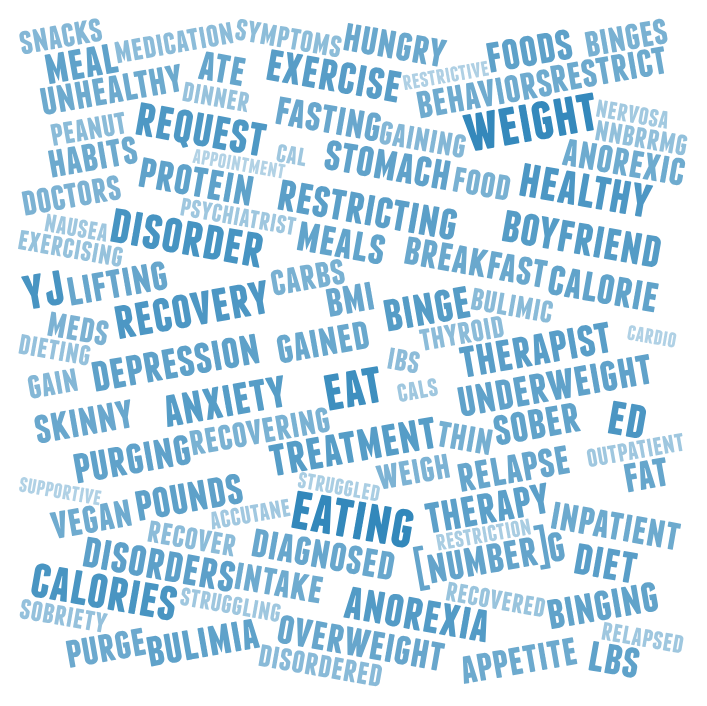
\includegraphics[width=.7\textwidth]{images/anorexia(gv)}
    \caption{Top 100 palabras seleccionadas por el \emph{valor global} aprendido para la clase positiva (anorexia) de la tarea 1.
    El tamaño de cada palabra se corresponde con su respectivo valor.}
    \label{fig:word-cloud-t1}
    \end{figure}
    Finalmente, es importante mencionar que estos resultados implican dos puntos relevantes: (a) la \emph{puntuación}\footnote{Véase \autoref{eq:puntuacion}.} generada por SS3 está estimando el nivel de riesgo de los sujetos correctamente, en otras palabras, efectivamente el \emph{valor global}, dado por $gv(w, c)$, está capturando correctamente el grado de importancia de las palabras ---lo que también se puede comprobar desde un punto de vista más cualitativo, como en los capítulos anteriores, por medio de una nube de palabras como la mostrada en la \autoref{fig:word-cloud-t1}; y más importante aún, (b) el hecho de que se esté estimando el nivel de riesgo de los usuarios correctamente implica que SS3 tiene mucho margen de mejora para las medidas centradas en la decisión, $ERDE$ y $F_{latency}$, si se utiliza una mejor política de clasificación anticipada ---ya que nos señala que si no se obtuvieron mejores resultados no se debió a una mala estimación del riesgo del usuario, sino a la política utilizada para decidir \emph{cuándo} clasificarlo en base a dicha estimación.
    Este último aspecto no es secundario, ya que permite identificar posibles líneas de trabajo para extender y mejorar el modelo a futuro, como se verá luego en el \autoref{cap:conclusion}.
\end{itemize}


\subsection{Tarea 2: Detección Anticipada de Conductas Autodestructivas}%Task 2: Early Detection of Signs of Self-harm



\begin{table*}[t]
\centering
\caption{Estadísticas principales del conjunto de prueba de la tarea 2.}
\label{tab:dataset-t2}
\begin{tabular}{l c c}
\hline
& Cond. Autodestructiva & Control \\ \hline
No. de sujetos & 41 & 299 \\
No. de publicaciones & 6927 & 163506 \\
Prom. de publicaciones por sujeto & 169.0 & 546.8 \\
Prom. de días (primera a última publ.) & 495 & 500 \\
Prom. de palabras por publicación & 24.8 & 18.8 \\ \hline

\hline
\end{tabular}
\end{table*}


En esta tarea participaron un total de 8 equipos de investigación distintos, y se enviaron un total de 29 modelos diferentes.
Como se describe más detalladamente en la descripción general del eRisk~\cite{losadaetal2019}, a diferencia de la tarea anterior, aquí no se proporcionó ningún conjunto de datos para entrenar a los modelos.
La evaluación de los modelos se llevó a cabo utilizando un conjunto de prueba construido con la misma metodología utilizada previamente, es decir, recolectando las publicaciones de un conjunto de usuarios de Reddit divididos en dos grupos, aquellos con conductas autodestructivas y aquellos que no.
En particular, para esta tarea, el grupo de riesgo se compuso por usuarios que habían participado activamente en el foro de conductas autodestructivas\footnote{En inglés, ``self-harm''.} de Reddit, y que además habían mencionado explícitamente que se habían autolesionado, por ejemplo, mediante cortes.
Sin embargo, en esta tarea se buscó poner a prueba, aún más, la capacidad de los modelos para detectar los casos lo antes posible ya que el conjunto de prueba sólo estuvo conformado por publicaciones realizadas antes del primer ingreso del usuario a dicho foro. %---la hipótesis detrás de esta decisión fue que un individuo que está activo en foros de autolesiones tal vez ya se ha autolesionado de alguna manera. %queremos algoritmos que detecten los casos antes y no cuando los casos son explícitos y el individuo ya está participando en un foro de apoyo. 
En la \autoref{tab:dataset-t2} se brindan las principales estadísticas de este conjunto de prueba.

\

Al igual que en la tarea anterior, la participación en esta tarea se llevó a cabo utilizando 5 modelos SS3 distintos.
Como se detalló en la \autoref{sec:erisk2019implementacion}, aquí también se utilizaron los mismos valores de hiperparámetros para los modelos, siendo los datos utilizados para entrenarlos la principal diferencia entre ellos.
Además, debido a la falta de un conjunto de entrenamiento, se tuvieron que crear manualmente diferentes conjuntos de datos, por ejemplo, recopilando tweets o publicaciones de Reddit relacionadas con la autolesión, como se detalla a continuación:

\begin{itemize}
% \item \emph{UNSL\#0}: modelo SS3 original entrenado con el conjunto de entrenamiento del eRisk 2018, excluyéndose así del entrenamiento a los usuarios correspondientes al conjunto de prueba de esa misma edición.
% De esta manera, el modelo obtenido se correspondió al utilizado en el capítulo anterior, permitiendo evaluar la consistencia y robustez de los resultados en relación a los obtenidos previamente en la experimentación controlada.
\item \emph{UNSL\#0}: modelo SS3 original entrenado con un conjunto de entrenamiento construido manualmente recopilando publicaciones individuales de Reddit, relacionadas con conductas autodestructivas.
Estas publicaciones fueron agrupadas y almacenadas en un único archivo de texto que representó a toda la clase positiva.\footnote{Esto fue posible dado que SS3 ``ve'' a cada clase como ``un único gran documento'', lo que además nos permitió construir el conjunto de datos propiamente dicho, ya que fue posible construirlo utilizando, en lugar de usuarios en riesgo, publicaciones individuales relacionadas a conductas autodestructivas.}
Además, como clase negativa, se utilizó el grupo de control del conjunto de entrenamiento de la tarea anterior.

\item \emph{UNSL\#1}: análogo al modelo anterior pero utilizando $\tau$-SS3 en lugar de SS3.

\item \emph{UNSL\#2}: modelo SS3 original entrenado con el conjunto de entrenamiento utilizado en los modelos anteriores, pero ampliándolo recolectando tweets relacionados a conductas autodestructivas (tweets con el hashtag ``\#selfharm'').
Además, al igual que con UNSL\#4 de la tarea anterior, este modelo sólo tuvo en cuenta las palabras con un \emph{valor global} mayor a $0.3$, durante el proceso de clasificación.

\item \emph{UNSL\#3}: modelo SS3 estándar entrenado con la unión de los conjuntos de entrenamiento de la tarea anterior (anorexia) y el de la tarea de depresión del eRisk 2018.
Esta variante fue pensada con el objetivo de poder analizar en qué medida la información aprendida en base a usuarios con anorexia y depresión, de forma conjunta, también le permite a SS3 detectar usuarios con conductas autodestructivas ---ya que estos tres trastornos suelen estar estrechamente vinculados.

\item \emph{UNSL\#4}: análogo al modelo anterior pero ampliando el conjunto de entrenamiento al unirlo con el utilizado en UNSL\#0.
Esta variante permite medir, en relación al modelo anterior, qué tanto impacta en el desempeño la incorporación de publicaciones específicas sobre conductas autodestructivas.

\end{itemize}


\begin{figure*}[t!]
    \begin{subfigure}{0.5\textwidth}
        \centering
        
\includegraphics[width=\textwidth]{images/selfharm(gv)}
        \caption{Palabras}
        % \label{fig:word_cloud_a}
    \end{subfigure}
    \begin{subfigure}{0.5\textwidth}
        \centering
        
\includegraphics[width=\textwidth]{images/selfharm_bigrams(gv)}
        \caption{Bigramas}
        % \label{fig:word_cloud_b}
    \end{subfigure}
\caption{
    Top 100 palabras y bigramas seleccionados por el \emph{valor global} aprendido por, respectivamente, los modelos \emph{UNSL\#0} y \emph{UNSL\#1} de la tarea 2, detección de conductas autodestructivas.
    El tamaño de cada elemento se corresponde con su respectivo \emph{valor global}.
}
\label{fig:word_cloud_t2}
\end{figure*}

Al no contar con ningún tipo de conjunto de validación real, luego de que los modelos fueron entrenados, se los utilizó para generar una lista ordenada con los pares (palabra, \emph{valor global}) aprendidos por cada modelo.
A continuación, cada lista se revisó manualmente para corroborar que las palabras y valores aprendidos tuvieran cierto sentido en relación a la tarea sobre la que finalmente iban a ser evaluados.
Afortunadamente, a pesar de haber utilizado los mismos hiperparámetros en todos los modelos, las listas generadas coincidieron con lo esperado, como lo ilustran las nubes de palabras de la \autoref{fig:word_cloud_t2}.
Notar que este procedimiento de inspección manual fue posible gracias a que la transparencia y la simpleza formaron parte de los objetivos de diseño del modelo.\footnote{Ya que pocos son los modelos que permitirían, de forma simple y transparente, abordar preguntas tales como ``¿qué tan bien aprendió el modelo?¿qué tanto sentido tiene lo aprendido?'', sin la disponibilidad y el uso de un conjunto de validación sobre el que medir el desempeño.}


\vspace{5mm}

En relación a la tarea anterior, la efectividad general de todos los participantes fue menor en esta tarea.
Esto se debió a que, como se esperaba, la tarea representó un mayor reto para los modelos ya que, como se mencionó, no sólo no se proporcionaron datos de entrenamiento sino que la evidencia relacionada a las autolesiones podría ser muy escasa o, en muchos casos, incluso estar ausente ---ya que el conjunto de prueba no contó con ningún tipo de publicación creada luego de que los usuarios hayan decidido ingresar al foro de conductas autodestructivas.
% A continuación se presentarán los resultados obtenidos para esta tarea,
% Así, los principales resultados obtenidos con los 5 modelos descritos anteriormente, agrupados según las medidas utilizadas para medir el desempeño de los mismos, son los siguientes:
Los principales resultados obtenidos con los 5 modelos descritos anteriormente, agrupados según las medidas utilizadas para medir el desempeño de los mismos, son los siguientes:
% Los principales resultados globales obtenidos en esta tarea, tanto para las medidas centradas en la decisión como las basadas en ranking, se podrían resumir de la siguiente manera:


\begin{table*}[t!]
\centering
\caption{Resultados obtenidos en la tarea 2 para las medidas centradas en la decisión. A modo de comparación, del total de 29 modelos participantes, aquí se muestran, ordenados por $ERDE_{50}$, sólo los modelos que obtuvieron los mejores valores de cada uno de los otros 7 equipos de investigación.}
\label{tab:t2-result}
\begin{tabular}{l c c c c c}
\hline
Equipo\#modelo & $ERDE_5$ & $ERDE_{50}$ & $F_{latency}$ \\ \hline

UNSL\#0 & 9.01\% & 7.31\% & \textbf{.52} \\
UNSL\#1 & 9.03\% & 7.60\% & .50 \\
UNSL\#2 & 9.20\% & 6.86\% & .32 \\
UNSL\#3 & 8.79\% & 5.44\% & .45 \\
UNSL\#4 & \textbf{8.21\%} & \textbf{4.93\%} & .45 \\
\hline
\hline
BiTeM\#0 & 9.73\% & 7.63\% & .46 \\
BioInfo@UAVR\#0 & 10.79\% & 8.11\% & .45 \\
UDE\#2 & 13.75\% & 9.56\% & .28 \\
UDE\#1 & 11.27\% & 9.80\% & .29 \\
lirmm\#0 & 12.22\% & 10.02\% & .35 \\
CAMH\#4 & 14.84\% & 10.32\% & .22 \\
lirmm\#1 & 12.18\% & 10.58\% & .29 \\
LTL-INAOE\#2 & 12.53\% & 10.60\% & .22 \\
Fazl\#2 & 22.66\% & 13.23\% & .19 \\
Fazl\#1 & 22.66\% & 16.42\% & .18 \\
\hline

\end{tabular}
\end{table*}

\begin{itemize}
    % UNSL\#0 - Entre todos los participantes, este modelo obtuvo el mejor $F_{latency}$ ($.52$) y el mejor \emph{precision} ($.71$). Sin embargo, comparado con nuestros otros modelos, fue el que obtuvo el \emph{recall} más bajo ($.41$), junto con UNSL\#1 ($.39$), el cual también utilizó este mismo conjunto de datos.
    % UNSL\#2 - Este modelo obtuvo, de entre nuestros modelos, el mejor \emph{recall} ($.9$) pero los peores valores de \emph{precision} ($.2$) y $F_1$ ($.32$).
    % UNSL\#3 - Notablemente, el desempeño obtenido fue muy similar al del siguiente modelo, el cual obtuvo los mejores $ERDE_5$ y $ERDE_{50}$.

    

    \item \textbf{Desempeño centrado en la decisión:} en la \autoref{tab:t2-result} se muestran los resultados obtenidos para las medidas centradas en la decisión.
    En relación a las medidas $ERDE$ y $F_{latency}$, se puede observar que, de entre todos los participantes, el modelo \emph{UNSL\#4} obtuvo los mejores valores para $ERDE_5$ ($8.20\%$) y $ERDE_{50}$ ($4.93\%$), mientras que \emph{UNSL\#0} obtuvo el mejor valor $F_{latency}$ ($.52$). %\footnote{Además, si bien no se incluyen en esta tabla, este último también obtuvo los mejores \emph{precision} ($.71$) y $F_1$ ($.52$).}
    De entre los 5 modelos SS3, los dos entrenados con publicaciones individuales relacionadas a conductas autodestructivas, \emph{UNSL\#0 y \#1}, fueron los que mejor se desempeñaron en términos de la medida $F_{latency}$, pero los que obtuvieron el peor desempeñaron en términos de $ERDE_{50}$.
    Esto probablemente se haya debido a que estos modelos pudieron detectar con precisión a los usuarios cuya condición era más evidente (con publicaciones directamente vinculadas a conductas autodestructivas), pero dejando sin detectar a todos los otros usuarios en riesgo.\footnote{Esto también se vio reflejado en las medidas tradicionales, en donde \emph{UNSL\#0} obtuvo un $0.71$ de $precision$, pero un $0.41$ de $recall$.}
    Por lo tanto, dado que la medida de error $ERDE$ acumula más error cuando el modelo no detecta un caso en riesgo (falso negativo) que cuando detecta a uno que en realidad no lo era (falsos positivos), los errores $ERDE$ para estos modelos fueron mayores.
    Al igual que en la tarea anterior, y tal vez por los mismos motivos, el modelo $\tau$-SS3 (\emph{UNSL\#1}) obtuvo un desempeño ligeramente menor a su contraparte SS3 (\emph{UNSL\#0}) con este conjunto de datos.
    Por otro lado, el modelo \emph{UNSL\#2} fue el que obtuvo el peor desempeño de entre los 5 modelos, especialmente en las medidas $F_{latency}$ y $ERDE_5$, por lo que la incorporación de los tweets con hashtag ``\#selfharm'' al conjunto de entrenamiento produjo un impacto considerablemente negativo en el desempeño ---tal vez la información contenida en estos tweets aportó más ruido que información realmente útil para decidir si un usuario tiene conductas autodestructivas o no.
    En relación al modelo \emph{UNSL\#3}, entrenado con depresión y anorexia, obtuvo los segundos mejores valores $ERDE$ de entre todos los participantes, sólo por debajo del modelo \emph{UNSL\#4}, el cual también fue entrenado con depresión y anorexia pero ampliándolo con las publicaciones utilizadas para entrenar a los dos primeros modelos.
    Es importante resaltar que esto sugiere que, efectivamente, el vínculo con la depresión y la anorexia es lo suficientemente fuerte como para permitirle a SS3, en cierto grado, detectar usuarios padeciendo de conductas autodestructivas.
    Además, esto también podría sugerir que SS3 posee cierta robustez para lidiar con algunos escenarios de dominios cruzados.
    Esto último se ve reforzado por el hecho de que los modelos de UDE~\cite{masood2019ude} también fueron entrenados utilizando el mismo conjunto de entrenamiento que \emph{UNSL\#3}, anorexia y el depresión del eRisk 2018, y sin embargo, el desempeño de los mismos fue con diferencia más bajo que el de este último.
    Por ejemplo, \emph{UDE\#1} y \emph{UDE\#2} fueron los mismos modelos utilizados por UDE en la tarea anterior, estando el primero implementado con dos clasificadores SVM (uno utilizado para filtrar publicaciones no relevantes y otro para tomar la decisión final) y estando el segundo implementado con una red neuronal recurrente LSTM tomando como entrada un vector \emph{doc2vec} representando las publicaciones leídas hasta el momento.
    Sin embargo, \emph{UDE\#1} obtuvo un $ERDE_{50}$ de $9.80\%$ y un $F_{latency}$ de $0.29$, y \emph{UDE\#2} un $ERDE_{50}$ de $9.56\%$ y un $F_{latency}$ de $0.28$, mientras que \emph{UNSL\#3} obtuvo un error $ERDE_{50}$ considerablemente menor ($5.44\%$) y un $F_{latency}$ considerablemente mayor ($0.45$), habiendo sido entrenado con los mismos datos ---sugiriendo que SS3 se adaptó considerablemente mejor al cambio de dominio que los dos primeros, los cuales se (sobre)ajustaron al dominio original en el que fueron entrenados (anorexia y depresión).
    Como se verá luego en el \autoref{cap:conclusion}, este aspecto no es secundario y será considerado como línea de trabajo a ser explorada como trabajo a futuro.

\begin{table*}[t!]
\centering
\caption{Detalle de los equipos participantes en la tarea 2: nombre del equipo, cantidad de modelos empleados ($\#modelos$), número de publicaciones procesadas de los usuarios ($\#publicaciones$), tiempo total empleado para completar la tarea y tiempo empleado para procesar cada publicación (\emph{i.e.} $\frac{tiempo\ total}{\#publicaciones\times\#modelos}$).}%Participating teams for Task 2: number of runs, number of user writings processed by the team, and the time taken for the whole process and for processing each writing (i.e $\frac{TotalTime}{\#writings\times\#runs}$). (*) This value was originally 5, but we replaced it by the actual number of models used.
\label{tab:t2-time}
\begin{tabular}{l c c|c | c}
\hline
& & & \multicolumn{2}{c}{Tiempo} \\
Equipo & \#modelos & \#publicaciones & total & por publicación  \\ \hline

\textbf{UNSL}$\star$ & 5 & 1992 & 13h & \textbf{4.6s} \\
BioInfo@UAVR & 1 & 1992 & 4h & 7.2s \\
LTL-INAOE & 4 & 1993 & 17h & 7.6s \\
BiTeM & 2 & 8 & 3m & 11.2s \\
UDE & 4 & 1992 & 1 día + 2h & 11.7s \\
CAMH & 5 & 1992 & 1 día + 19h & 15.5s \\
lirmm & 5 & 2004 & 2 días + 22h & 25.1s \\
Fazl & 3 & 1993 & 18 días + 21h & 4m + 32s \\

\hline
\end{tabular}
\end{table*}

    \item \textbf{Desempeño en relación al tiempo de ejecución:} en la \autoref{tab:t2-time} se muestran, por cada equipo, detalles sobre el tiempo total empleado para completar la tarea.
    Como se puede observar, a diferencia de la primer tarea, el tiempo empleado fue relativamente similar entre cada equipo, siendo Fazl la única excepción, habiéndole tomado 18 días y 21 horas completar la tarea.
    Nuevamente se puede observar que UNSL fue, aunque no por mucho, el equipo más eficiente en términos de tiempos de ejecución ya que procesó las 1992 publicaciones de cada usuario con cada uno de los 5 modelos en 13 horas, por lo que cada modelo procesó cada publicación en aproximadamente 4.6 segundos.
    % como se muestra en la \autoref{tab:t2-time}, en esta tarea también fuimos los más rápidos en procesar las publicaciones, procesando cada una en poco menos de 5 segundos, tomándonos 13 horas en total completar la tarea.
    % Notar que si bien a simple vista puede parecer que BioInfo@UAVR~\cite{trifan2019bioinfo} fue más rápido, al completar la tarea en 4 horas, también se debe tener en cuenta que tuvo que procesar y enviar 5 veces menos publicaciones y respuestas al servidor que nosotros ---ya que participaron con un único modelo.

\begin{table*}[t!]
\centering
\caption{Resultados obtenidos en la tarea 2 para las medidas basadas en ranking para 4 rankings distintos, respectivamente, el ranking obtenido luego de leer 1, 100, 500 y 1000 publicaciones. Aquí también se incluyen, a modo de comparación, los mejores resultados obtenidos por los otros 7 equipos.}
\label{tab:t2-result-ranking}
\begin{tabular}{l c c c|c c c}
\hline
& \multicolumn{3}{c}{1 publicación leída} & \multicolumn{3}{c}{100 publicaciones leídas} \\
Equipo\#modelo & P@10 & NDCG@10 & NDCG@100 &  P@10 & NDCG@10 & NDCG@100 \\ \hline

UNSL\#0 & .7 & .79 & .48 & \textbf{.9} & \textbf{.94} & .61 \\
UNSL\#1 & .6 & .74 & .48 & \textbf{.9} & \textbf{.94} & .60 \\
UNSL\#2 & .9 & .88 & .62 & .8 & .75 & .75 \\
UNSL\#3 & \textbf{1} & \textbf{1} & \textbf{.67} & \textbf{.9} & \textbf{.94} & .84 \\
UNSL\#4 & \textbf{1} & \textbf{1} & .64 & \textbf{.9} & .93 & \textbf{.86} \\
\hline\hline
Fazl\#1 & .2 & .27 & .36 & \textbf{.9} & \textbf{.94} & .83 \\
CAMH\#0 & .3 & .37 & .47 & .6 & .71 & .49 \\
UDE\#1 & .7 & .56 & .52 & .7 & .66 & .69 \\
CAMH\#2 & .3 & .41 & .51 & .5 & .62 & .39 \\
UDE\#2 & .5 & .63 & .53 & .5 & .56 & .64 \\
LTL-INAOE\#0 & .5 & .5 & .45 & .4 & .41 & .55 \\
LTL-INAOE\#1 & .6 & .73 & .56 & .1 & .19 & .17 \\
BiTeM\#4 & .4 & .56 & .50 & - & - & - \\
BiTeM\#2 & .5 & .48 & .44 & - & - & - \\
BiTeM\#0 & .3 & .35 & .53 & - & - & - \\
lirmm\#0 & .1 & .19 & .15 & 0 & 0 & .01 \\


\hline
\hline
\end{tabular}

\

\

\begin{tabular}{l c c c|c c c}
\hline
& \multicolumn{3}{c}{500 publicaciones leídas} & \multicolumn{3}{c}{1000 publicaciones leídas} \\
Equipo\#modelo & P@10 & NDCG@10 & NDCG@100 &  P@10 & NDCG@10 & NDCG@100 \\ \hline

UNSL\#0 & \textbf{.9} & \textbf{.94} & .66 & \textbf{.9} & \textbf{.94} & .66 \\
UNSL\#1 & \textbf{.9} & \textbf{.94} & .65 & \textbf{.9} & \textbf{.94} & .65 \\
UNSL\#2 & .5 & .59 & .74 & .6 & .64 & .74 \\
UNSL\#3 & .7 & .63 & .75 & .7 & .63 & .75 \\
UNSL\#4 & .7 & .67 & \emph{.79} & .8 & .74 & \emph{.78} \\
\hline\hline
Fazl\#1 & \textbf{.9} & \textbf{.94} & \textbf{.84} & \textbf{.9} & \textbf{.94} & \textbf{.84} \\
UDE\#1 & .8 & .75 & .74 & .8 & .75 & .74 \\
CAMH\#0 & .7 & .72 & .50 & .6 & .66 & .48 \\
CAMH\#2 & .7 & .72 & .45 & .6 & .66 & .44 \\
UDE\#2 & .6 & .66 & .68 & .6 & .65 & .67 \\
LTL-INAOE\#0 & .2 & .19 & .25 & .1 & .19 & .37 \\
LTL-INAOE\#1 & .1 & .06 & .07 & 0 & 0 & .04 \\

\hline
\hline
\end{tabular}

\end{table*}

    \item \textbf{Desempeño basado en ranking:} en la \autoref{tab:t2-result-ranking} se muestran los resultados obtenidos para las medidas basadas en ranking.
    Se puede observar que, si bien hubo una caída general en el desempeño de los modelos SS3 en relación a los obtenidos en la primer tarea, nuevamente se obtuvieron los mejores valores para las medidas $P@10$ y $NDCG@10$ en los 4 rankings y los mejores valores en la medida $NDCG@100$ para los rankings obtenidos luego de procesar $1$ y $100$ publicaciones, y el segundo mejor luego de procesar $500$ y $1000$ publicaciones.
    En relación al desempeño de las distintas variantes utilizadas, la principal diferencia se encuentra entre los modelos entrenados con publicaciones individuales (\emph{UNSL\#0 y \#1}) y los entrenados con depresión y anorexia (\emph{UNSL\#3 y \#4}), siendo los primeros mejores en términos de $P@10$ y $NDCG@10$, y los segundos en términos de $NDCG@100$.
    Esto posiblemente se deba a los mismos motivos expuestos anteriormente en relación al desempeño basado en decisión, en donde los primeros obtuvieron el mejor $F_{latency}$ y los segundos los mejores valores $ERDE$.\footnote{Los primeros son más precisos en detectar usuarios con mayor evidencia explícita, pero, a diferencia de los segundos, dejan a gran parte de los usuarios en riesgo sin detectar, pudiendo así armar un ranking de 10 usuarios pero fallando en armar un ranking mayor, de 100 usuarios, en donde todos los 61 usuarios en riesgo deberían estar presentes.}
    Finalmente, en relación al modelo entrenado con tweets, \emph{UNSL\#2}, al igual que con las medidas basadas en decisión, su desempeño fue el peor de entre los 5 modelos ---no obtuvo un mejor valor en ninguna medida y en ningún ranking.
    En líneas generales, es interesante notar que pese a haber sido entrenados con distintos conjuntos de datos, incluido datos de otros dominios, los modelos SS3 obtuvieron resultados consistentemente buenos en relación a los otros modelos, y más importante aún, a lo largo de los distintos tipos de medidas de desempeño utilizadas.
    Esto contrasta con otros modelos que si bien se desempeñaron bien en relación a ciertos aspectos de la problemática abordada, no lo hicieron robusta y consistentemente en relación a otros.
    Por ejemplo, el modelo \emph{Fazl\#1} obtuvo un buen desempeño en las medidas de ranking, obteniendo el mejor valor $NDCG@100$ para los rankings generados luego de leer 500 y 1000 publicaciones, sin embargo, como se observó en la \autoref{tab:t1-result}, obtuvo el peor desempeño de entre todos los modelos participantes en relación a las medidas centradas en la decisión, a pesar de haber demorado cerca de 19 días en completar la tarea.
    Finalmente, notar que al igual que en la tarea anterior, SS3 parece ser capaz de estimar el nivel de riesgo de los usuarios, con cierta eficiencia, aún cuando muy poca información ha sido procesada.
    Por ejemplo, como se observa en la sección ``1 publicación leída'' de la \autoref{tab:t2-result-ranking},
    todos los modelos obtuvieron mejores resultados que el resto de los modelos, a pesar de haber sido entrenados con distintos datos.
    Además, en relación a este último punto, es interesante destacar el hecho que los modelos \emph{UNSL\#3 y \#4} hayan sido capaces de construir un ranking ideal de 10 usuarios en riesgo (\emph{i.e.} $NDCG@10 = 1$) habiendo leído solamente la primer publicación de cada usuario.


\end{itemize}



% \subsection{Tarea 3: Medición de la Gravedad de la Depresión}%Task 3: Measuring the severity of the signs of depression

% participaron 8 equipos.

% %This task was really difficult since it was not a single ``yes or no'' problem but a problem involving multiple decisions, one for each one of the 21 questions. To make things even harder, as with Task 2, no training data was released either.
% Esta tarea fue realmente difícil ya que no se trataba de un solo problema de `` sí o no '' sino de un problema que involucraba múltiples decisiones, una para cada una de las 21 preguntas. Para hacer las cosas aún más difíciles, como con la Tarea 2, tampoco se publicaron datos de entrenamiento.
% %Fortunately, early depression detection is a task we had some previous experience working with since we had participated in the two previous eRisk labs (2017\cite{burdisso2019} and 2018\cite{funez2018}).
% Afortunadamente, la detección temprana de la depresión es una tarea con la que teníamos experiencia previa trabajando desde que habíamos participado en los dos laboratorios de eRisk anteriores (2017\cite{burdisso2019} y 2018\cite{funez2018}).
% %Therefore, we decided to train SS3 using the dataset for the eRisk 2018 depression detection task.
% Por lo tanto, decidimos entrenar SS3 utilizando el conjunto de datos para la tarea de detección de depresión eRisk 2018.
% %However, the main problem was deciding how to turn this ``yes or no'' classifier into a classifier capable of filling BDI questionnaires. We came up with the idea of using the \emph{confidence vector}, $\overrightarrow{d}$ in  \autoref{eq:sum_gv}, to somehow infer a BDI depression level between 0 and 63. To achieve this, first, we converted the \emph{confidence vector} into a single \emph{confidence value} normalized between 0 and 1, by applying the following equation:
% Sin embargo, el principal problema fue decidir cómo convertir este clasificador de `` sí o no '' en un clasificador capaz de llenar cuestionarios BDI. Se nos ocurrió la idea de usar el \emph{vector de confianza}, $\overrightarrow{d}$ en \autoref{eq:sum_gv}, para inferir de alguna manera un nivel de depresión del BDI entre 0 y 63. Para lograr esto, primero convertimos el \emph{vector de confianza} en un \emph{valor de confianza} único normalizado entre 0 y 1, aplicando la siguiente ecuación:

% \begin{equation}
%     confidence\_value = \frac{d[positive]-d[negative]}{d[positive]}
%     \label{eq:conf_val}
% \end{equation}

% % \begin{equation}
% %     depression\_level = \frac{d[positive]-d[negative]}{d[positive]}\times63
% % \end{equation}

% %Then, after SS3 classified a subject, the obtained $confidence\_value$ was divided into 4 regions, one for each BDI depression category. This was carried out by the following equation:
% Luego, después de que SS3 clasificara a un sujeto, la $confidence\_value$ obtenida se dividió en 4 regiones, una para cada categoría de depresión del BDI. Esto se llevó a cabo mediante la siguiente ecuación:

% \begin{equation}
%     c = \lfloor confidence\_value \times 4\rfloor
%     \label{eq:c}
% \end{equation}

% %And finally, the subject depression level was predicted by mapping the percentage of $confidence\_value$ left inside the predicted $c$ region to its corresponding BDI depression level range (e.g. $(0.5, 0.75]\longrightarrow[19,29]$ for $c = 2 =$ ``moderate depression'') by computing the following:
% Y finalmente, el nivel de depresión del sujeto se predijo mapeando el porcentaje de $confidence\_value$ que queda dentro de la región $c$ predicha a su rango de nivel de depresión BDI correspondiente (por ejemplo, $(0.5, 0.75]\longrightarrow[19,29]$ para $c = 2 =$ ``depresión moderada'') calculando lo siguiente:

% \begin{equation}
%     depression\_level = min_c + \lfloor(max_c - min_c + 1) \times (confidence\_value \times 4 - c)\rfloor
%     \label{eq:dep_lvl}
% \end{equation}
% %Where $min_c$ and $max_c$ are the lower and upper bound for category $c$,  respectively (e.g. 19 and 29 for ``moderate depression'' category). 
% Donde $min_c$ y $max_c$ son el límite inferior y superior para la categoría $c$, respectivamente (por ejemplo, 19 y 29 para la categoría de `` depresión moderada '').


% \begin{figure}[t!] % [t]op; [h]ere; [p]age; [b]ottom; [r]ight; [l]eft
%     \centering
%     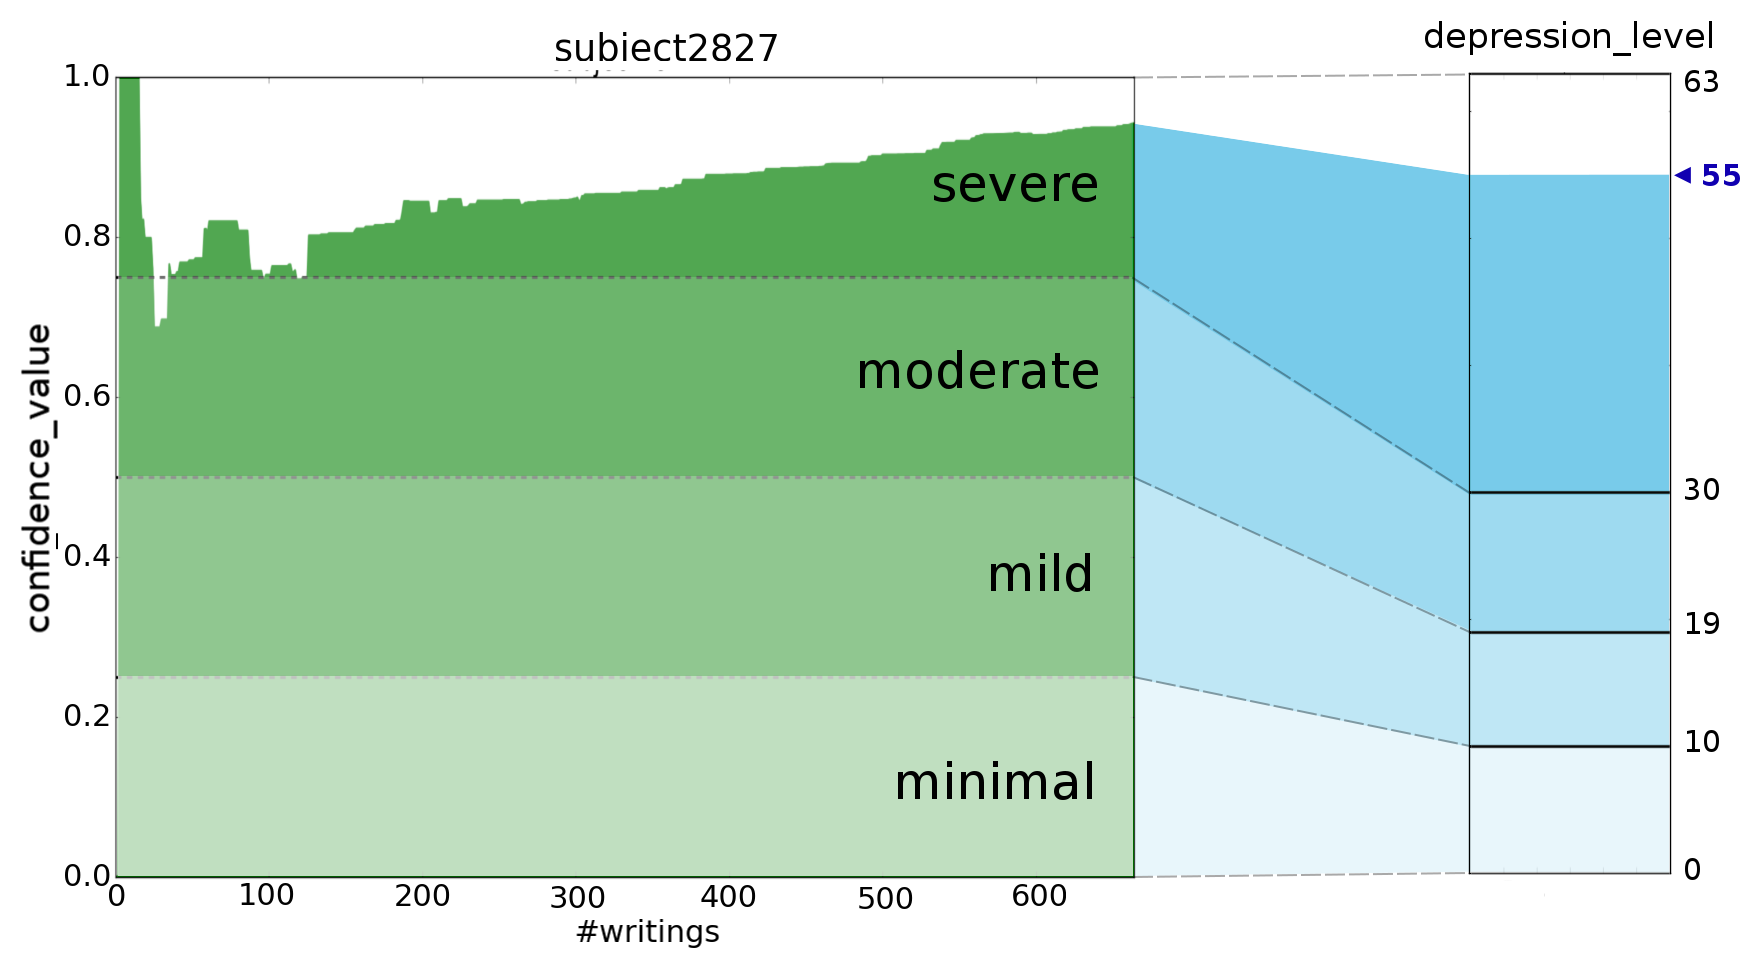
\includegraphics[width=120mm]{images/subject2827-bdi}
%     \caption{Diagrama del proceso de cálculo de \emph{depression\_level} para el sujeto 2827. Como puede notar el lector, después de procesar todos los escritos del sujeto, el \emph{confidence\_value} (0,941) final se mapeó en su \emph{depression\_level} (55) correspondiente.}%Diagram of the \emph{depression\_level} computation process for subject 2827. As reader can notice, after processing all the subject's writings, the final \emph{confidence\_value} (0.941) was mapped into its corresponding \emph{depression\_level} (55).
%     \label{fig:subject-bdi}
% \end{figure}

% \vspace{5mm}

% \begin{figure*}[t!]
%     \begin{subfigure}{0.5\textwidth}
%         \centering
%         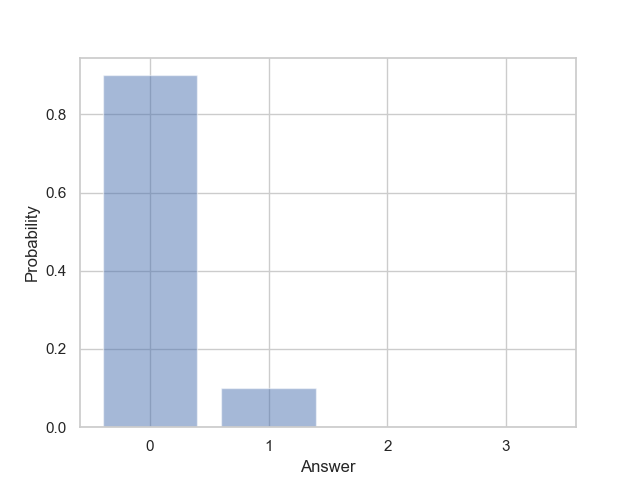
\includegraphics[width=65mm]{images/distp-exp0.png}
%         \caption{If expected answer is 0}
%     \end{subfigure}
%     \begin{subfigure}{0.5\textwidth}
%         \centering
%         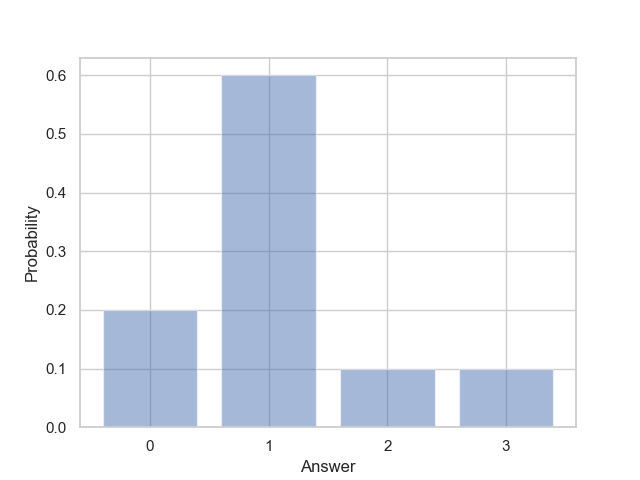
\includegraphics[width=65mm]{images/distp-exp1.png}
%         \caption{If expected answer is 1}
%     \end{subfigure}
%     \begin{subfigure}{0.5\textwidth}
%         \centering
%         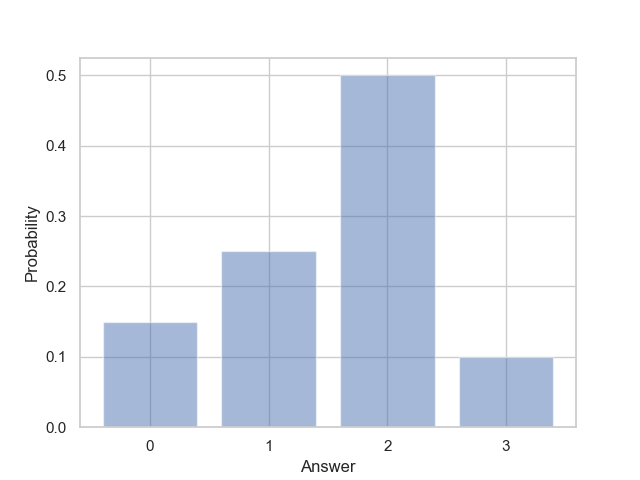
\includegraphics[width=65mm]{images/distp-exp2.png}
%         \caption{If expected answer is 2}
%     \end{subfigure}
%     \begin{subfigure}{0.5\textwidth}
%         \centering
%         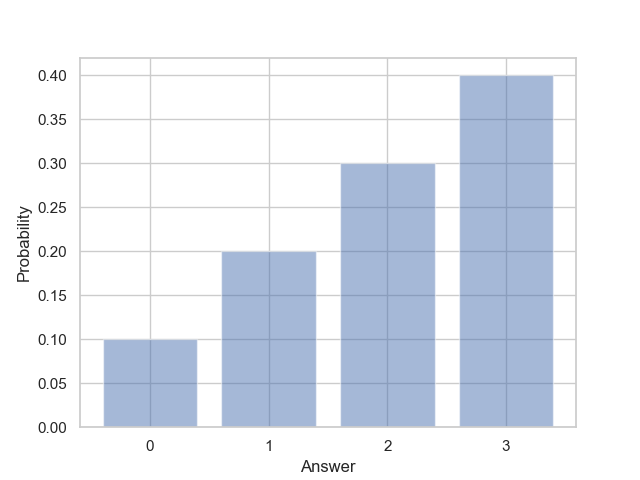
\includegraphics[width=65mm]{images/distp-exp3.png}
%         \caption{If expected answer is 3}
%     \end{subfigure}
% \caption{
%     Distribución de probabilidad discreta para cada posible respuesta esperada.
% }%Discrete probability distribution for each possible expected answer.
% \label{fig:distprob-t3}
% \end{figure*} 

% %In order to clarify the above process, we will illustrate it with the example shown in \autoref{fig:subject-bdi}. First, SS3 processed the entire writing history computing the $confidence\_value$ (given by \autoref{eq:conf_val}) and then, the final $confidence\_value$ (0.941) was used to predict the depression category, ``severe depression'' ($c = 3$), by using the \autoref{eq:c}. Finally, the depression level was computed by the mapping given by \autoref{eq:dep_lvl}, as follows:
% Para aclarar el proceso anterior, lo ilustraremos con el ejemplo que se muestra en \autoref{fig:subject-bdi}. Primero, SS3 procesó todo el historial de escritura calculando el $confidence\_value$ (dada por \autoref{eq:conf_val}) y luego, el $confidence\_value$ final (0.941) se usó para predecir la categoría de depresión, `` depresión severa '' ($c = 3$), usando la \autoref{eq:c}. Finalmente, el nivel de depresión se calculó mediante el mapeo proporcionado por \autoref{eq:dep_lvl}, de la siguiente manera:

% \begin{equation}
%     \begin{split}
%     depression\_level & = 30 + \lfloor(63 - 30 + 1) \times (0.941\times4 - 3)\rfloor \\
%     & = 
%     30 + \lfloor34 \times (3.764 - 3)\rfloor = 30 + \lfloor34 \times 0.764\rfloor \\
%     & = 30 + 25 = \textbf{55}
%     \end{split}
% \end{equation}



% %At this point, we have transformed the output of SS3 from a 2-dimensional vector, $d$, into a BDI depression level (a value between 0 and 63).
% En este punto, hemos transformado la salida de SS3 de un vector bidimensional, $d$, a un nivel de depresión BDI (un valor entre 0 y 63).
% %However, we have not covered yet how to actually answer the 21 questions in the BDI questionnaire using this \emph{depression level}.
% Sin embargo, todavía no hemos cubierto cómo responder realmente a las 21 preguntas del cuestionario BDI utilizando este \emph{nivel de depresión}.
% %Regardless of the method, we decided that for all those users whose $depression\_level$ was less or equal to 0, all the BDI questions were answered with 0. For the other users we applied different methods, depending on the run, as described below:
% Independientemente del método, decidimos que para todos aquellos usuarios cuyo $depression\_level$ fuera menor o igual a 0, todas las preguntas de BDI se respondieran con 0. Para los demás usuarios aplicamos diferentes métodos, según la ejecución, como se describe a continuación:

% \begin{itemize}
%     %\item \emph{UNSLA}: using the predicted \emph{depression\_level} our model filled the questionnaires answering the expected number ($\lfloor\frac{depression\_level}{21}\rfloor$) on each question. If this division had a remainder, the remainder points were randomly scattered so that the sum of all the answers always matched the predicted depression level given by SS3.
%     \item \emph{UNSLA}: utilizando el \emph{depression\_level} predicho, nuestro modelo llenó los cuestionarios respondiendo el número esperado ($\lfloor\frac{depression\_level}{21}\rfloor$) en cada pregunta. Si esta división tenía un resto, los puntos restantes se dispersaron aleatoriamente para que la suma de todas las respuestas siempre coincidiera con el nivel de depresión predicho dado por SS3.
%     %\item \emph{UNSLB}: this time, only the predicted category, $c$, was used. Our model filled the questionnaire randomly in such a way that the final depression level always matched the predicted category. Compared to the following three ones, these two models were the ones with the worst performance.
%     \item \emph{UNSLB}: esta vez, sólo se utilizó la categoría predicha, $c$. Nuestro modelo llenó el cuestionario al azar de tal manera que el nivel de depresión final siempre coincidió con la categoría prevista. En comparación con los siguientes tres, estos dos modelos fueron los que presentaron el peor rendimiento.
%     %\item \emph{UNSLC}: this model and the followings were more question-centered.
%     \item \emph{UNSLC}: este modelo y los siguientes estaban más centrados en preguntas.
%     %Once again, as in UNSLA, our model filled the questionnaires answering the expected number derived from the predicted depression level ($\lfloor\frac{depression\_level}{21}\rfloor$). But this time, answering this number only on questions for which a ``textual hint'' for a possible answer was found in the user's writings, and randomly and uniformly answered between 0 and $\ceil[big]{\frac{depression\_level}{21}}$ otherwise. To find this ``textual hint'', our model split the user's writings into sentences and searched for the co-occurrence of the word ``I'' or ``my'' with at least one word matching a regular expression specially crafted for each question.\footnote{e.g. ``(sad)$|$(unhappy)'' for question 1, ``(future)$|$(work out)'' for question 2, ``fail\textbackslash w*'' for question 3, ``(pleasure)$|$(enjoy)'' for question 4, etc. } This method obtained the best AHR (41.43\%) and the second-best DCHR (40\%).
%     Una vez más, como en UNSLA, nuestro modelo llenó los cuestionarios respondiendo el número esperado derivado del nivel de depresión pronosticado ($\lfloor\frac{depression\_level}{21}\rfloor$). Pero esta vez, respondiendo a este número solo en preguntas para las que se encontró una ``pista textual'' para una posible respuesta en los escritos del usuario, y se respondió de manera aleatoria y uniforme entre 0 y $\ceil[big]{\frac{depression\_level}{21}}$ en caso contrario. Para encontrar esta ``pista textual'', nuestro modelo dividió los escritos del usuario en oraciones y buscó la co-ocurrencia de la palabra ``I'' o ``my'' con al menos una palabra que coincida con una expresión regular especialmente diseñada para cada pregunta.\footnote{p.ej. ``(triste)$|$(infeliz)'' para la pregunta 1, ``(futuro)$|$(resolver)'' para la pregunta 2, ``fail\textbackslash w*'' para la pregunta 3, ``(placer)$|$(disfrutar)'' para la pregunta 4, etc.} Este método obtuvo el mejor AHR (41,43\%) y el segundo mejor DCHR (40\%).
    
%     %\item \emph{UNSLD}: the same as the previous one, but not using the ``textual hints'',  i.e. always answering every question randomly and uniformly between 0 and $\ceil[big]{\frac{depression\_level}{21}}$. This model was mainly used only with the goal of measuring the actual impact of using these ``textual hints'' to decide which questions should be answered with the expected answer ($\lfloor\frac{depression\_level}{21}\rfloor$).
%     \item \emph{UNSLD}: el mismo que el anterior, pero sin utilizar las ``pistas textuales'', es decir, siempre respondiendo todas las preguntas de forma aleatoria y uniforme entre 0 y $\ceil[big]{\frac{depression\_level}{21}}$. Este modelo se utilizó principalmente solo con el objetivo de medir el impacto real de utilizar estas ''sugerencias textuales'' para decidir qué preguntas deben responderse con la respuesta esperada (F$\lfloor\frac{depression\_level}{21}\rfloor$).
%     %\item \emph{UNSLE}: the same as UNSLD, but this time not using a uniform distribution. More precisely, from the overall depression level predicted by SS3, once again the expected answer was computed ($\lfloor\frac{depression\_level}{21}\rfloor$) and, depending on the value of the expected answer, actual answers were given following the probability distributions shown in \autoref{fig:distprob-t3}. Note that, unlike uniform distribution (used in UNSLD), when using these probability distributions the expected answer is more likely to be selected over the other ones. This model obtained the best ACR (71.27\%) and the second-best AHR (40.71\%) and ADODL (80.48\%, best was only 0.54\% above).
%     \item \emph{UNSLE}: lo mismo que UNSLD, pero esta vez sin utilizar una distribución uniforme. Más precisamente, a partir del nivel de depresión general predicho por SS3, una vez más se calculó la respuesta esperada ($\lfloor\frac{depression\_level}{21}\rfloor$) y, dependiendo del valor de la respuesta esperada, las respuestas reales se dieron siguiendo las distribuciones de probabilidad mostradas en \autoref{fig:distprob-t3}. Tenga en cuenta que, a diferencia de la distribución uniforme (utilizada en UNSLD), cuando se utilizan estas distribuciones de probabilidad, es más probable que se seleccione la respuesta esperada sobre las otras. Este modelo obtuvo el mejor ACR (71,27\%) y el segundo mejor AHR (40,71\%) y ADODL (80,48\%, el mejor fue solo un 0,54\% por encima).
% \end{itemize}

% \begin{table*}[t!]
% \centering
% \caption{Resultados de la tarea T3. para referencia, al final se ha añadido el promedio de completar el formulario al azar 1000 veces. }
% \label{tab:t3-result}
% \begin{tabular}{l c c c c}
% \hline
% Modelo & AHR & ACR & ADODL & DCHR \\ \hline

% UNSLA & 37.38\% & 67.94\% & 72.86\% & 30\% \\
% UNSLB & 36.93\% & 70.16\% & 76.83\% & 30\% \\
% UNSLC & \textbf{41.43\%} & 69.13\% & 78.02\% & \emph{40\%} \\
% UNSLD & 38.10\% & 67.22\% & 78.02\% & 30\% \\
% UNSLE & 40.71\% & \textbf{71.27\%} & \emph{80.48\%} & 35\% \\
% CAMH unsupervised & 23.81\% & 57.06\% & \textbf{81.03\%} & \textbf{45\%} \\
% CAMH supervised (SVM - LIWC) & 35.95\% & 66.59\% & 75.48\% & 25\% \\
% CAMH supervised (GPT - 180 features) & 35.47\% & 68.33\% & 75.63\% & 20\% \\
% CAMH supervised (GPT - 768 features) & 36.43\% & 67.22\% & 72.30\% & 20\% \\
% CAMH supervised (GPT - 948 features) & 36.91\% & 69.13\% & 75.63\% & 15\% \\
% BioInfo@UAVR & 34.05\% & 66.43\% & 77.70\% & 25\% \\
% BiTeM & 32.14\% & 62.62\% & 72.62\% & 25\% \\
% Fazl & 22.38\% & 56.27\% & 72.78\% & 5\% \\
% Illinois & 22.62\% & 56.19\% & 66.35\% & 40\% \\
% ISIKol multiSimilarity-5000-Dtac-Qtac & 29.76\% & 57.94\% & 74.13\% & 25\% \\
% ISIKol-bm25-1.2-0.75-5000-Dtac-Qtac & 29.76\% & 57.06\% & 72.78\% & 25\% \\
% ISIKol-lm-d-1.0-5000-Dtac-Qtac & 30.00\% & 57.94\% & 73.02\% & 15\% \\
% Kimberly & 38.33\% & 64.44\% & 66.19\% & 20\% \\
% \hline
% \hline
% Al Azar (promedio de 1000 repeticiones) & 23.98\% & 58.55\% & 77.78\% & 33.55\% \\
% \hline
% \end{tabular}
% \end{table*}

% \begin{table*}[t!]
% \centering
% \caption{Resultados de la Tarea 3. Ahora los resultados de nuestras ejecuciones se muestran utilizando un intervalo de confianza del 95\%.}%Results for Task 3. Now our runs results are shown using a 95\% confidence interval.
% \label{tab:t3-result-mean}
% \centerline{
% \begin{tabular}{l c c c c}
% \hline
% Modelo & AHR & ACR & ADODL & DCHR \\ \hline

% %CAMH\_GPT\_nearest\_unsupervised & 23.81\% & 57.06\% & 81.03\% & \textbf{45\%} \\
% UNSLA & 38.13\% $\pm$ 2.29\% & 68.30\% $\pm$ 0.84\% & 72.62\% & 30\% \\
% UNSLB & 38.97\% $\pm$ 2.65\% & \textbf{69.77\% $\pm$ 1.98\%} & 74.72\% $\pm$ 2.82\% & 30\% \\
% UNSLC & \textbf{40.19\% $\pm$ 3.14\%} & 69.26\% $\pm$ 1.75\% & 77.53\% $\pm$ 1.92\% & 29.91\% $\pm$ 8.70\% \\
% UNSLD & 39.26\% $\pm$ 3.21\% & 68.72\% $\pm$ 1.81\% & 77.56\% $\pm$ 1.86\% & 30.86\% $\pm$ 11.14\% \\
% UNSLE & 38.18\% $\pm$ 3.41\% & 69.61\% $\pm$ 1.95\% & \textbf{82.94\% $\pm$ 2.17\%} & \textbf{38.42\% $\pm$ 10.14\%} \\
% \hline
% \end{tabular}}
% \end{table*}

% % \begin{figure*}[t!]
% %     \begin{subfigure}{0.5\textwidth}
% %         \centering
% %         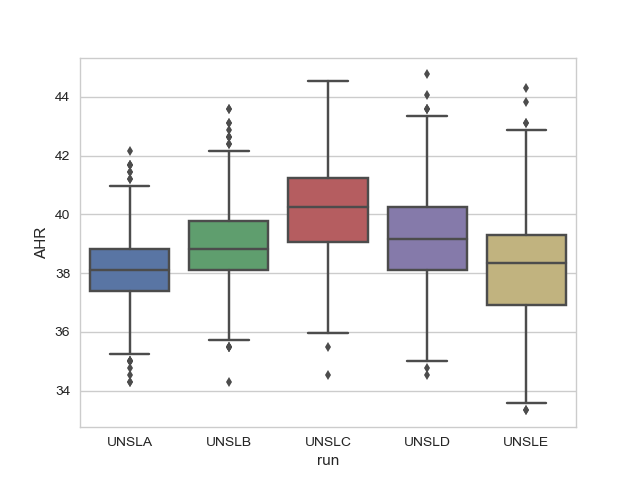
\includegraphics[width=68.5mm]{images/AHR}
% %         \caption{AHR}
% %         \label{fig:plot-result-t3-ahr}
% %     \end{subfigure}
% %     \begin{subfigure}{0.5\textwidth}
% %         \centering
% %         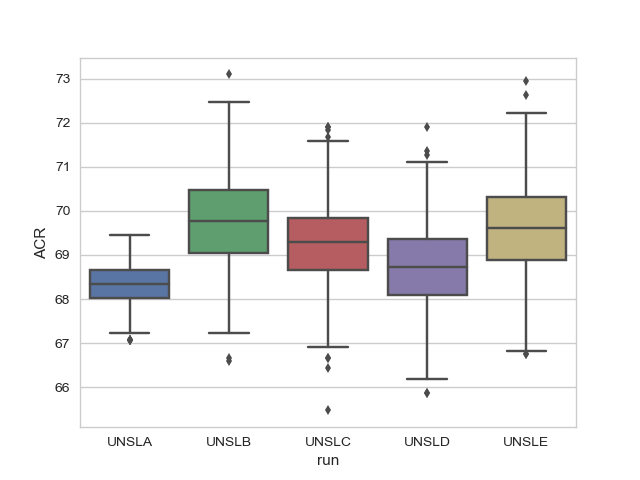
\includegraphics[width=68.5mm]{images/ACR}
% %         \caption{ACR}
% %     \end{subfigure}
% %     \begin{subfigure}{0.5\textwidth}
% %         \centering
% %         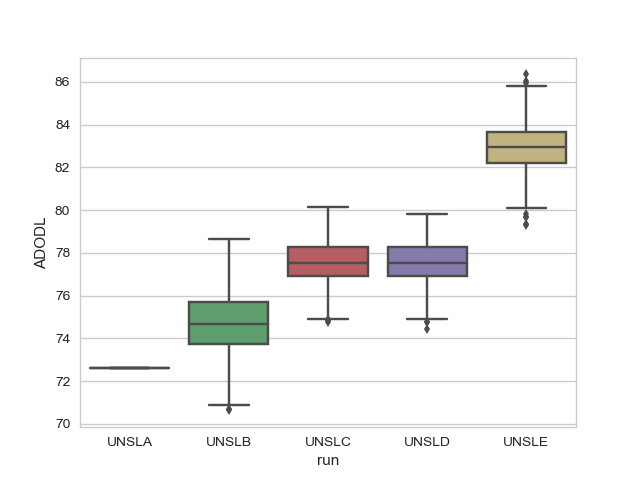
\includegraphics[width=68.5mm]{images/ADODL}
% %         \caption{ADODL}
% %         \label{fig:plot-result-t3-adodl}
% %     \end{subfigure}
% %     \begin{subfigure}{0.5\textwidth}
% %         \centering
% %         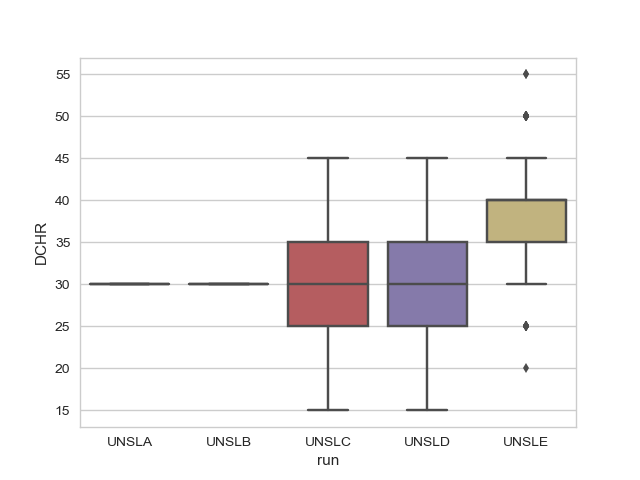
\includegraphics[width=68.5mm]{images/DCHR}
% %         \caption{DCHR}
% %     \end{subfigure}
% % \caption{
% %     Box plots for each measure and run.
% % }
% % \label{fig:plot-result-t3}
% % \end{figure*} 

% %The obtained results are shown in \autoref{tab:t3-result}. As mentioned above, we obtained the best AHR (41.43\%) and ACR (71.27\%), and the second-best ADODL (80.48\%) and DCHR (40\%). However, since most of our models' answers are randomly generated, it implies that all of these measures are also stochastically generated.\footnote{Only ADODL and DCHR for UNSLA and 
% Los resultados obtenidos se muestran en \autoref{tab:t3-result}. Como se mencionó anteriormente, obtuvimos el mejor AHR (41.43\%) y ACR (71.27\%), y el segundo mejor ADODL (80.48\%) y DCHR (40\%). Sin embargo, dado que la mayoría de las respuestas de nuestros modelos se generan aleatoriamente, esto implica que todas estas medidas también se generan estocásticamente.\footnote{Solo ADODL y DCHR para UNSLA y 
% %DHR for UNSLB are deterministically determined by $depression_level$ and $c$.} The natural question in cases like this is ``How do we know these results properly represent our models' performance and we did not obtain them just by pure chance?''. In order to clarify this, we run each model 1000 times and calculated the values for AHR, ACR, ADODL and DCHR each time\footnote{Just as if we had participated 1000 times in this task.}. After this process finished, we ended up with a sample of 1000 values for each measure and model, which we then used to produce the results shown in \autoref{tab:t3-result-mean}. Results have been replaced by intervals with 95\% of confidence, which better represent our performance. One can notice that, in fact, when we participated we had a little bit of bad luck, especially for UNSLE's ADODL, because the actual value we obtained (80.84\%) is almost a lower bound outlier. Another thing that we can notice, comparing UNSLC and UNSLD, is that the use of ``textual hints'' slightly improves the Average Hit Rate (AHR) but does not impact on the other measures. UNSLE is considerably the best method to estimate the overall depression level since it takes values within a range that is quite above the others. Additionally, another important point is that taking into account these 95\% confidence intervals, the obtained values would be among the best ones even in the worst cases. Finally, since all the methods we used are based on the depression level predicted by SS3, this shows us that SS3 is correctly inferring the depression level from the textual evidence accumulated while processing the user's writings, i.e. SS3 is correctly valuing words in relation to each category (depressed and non-depressed) which is consistent with the results obtained for the ranking-based measures for task T1 and T2. Additionally, this could also imply that could really be a relationship between how subjects write (what words they use) and the actual depression level they have.
% DHR para UNSLB están determinados determinísticamente por $depression_level$ y $c$.} La pregunta natural en casos como este es ``¿Cómo sabemos que estos resultados representan correctamente el rendimiento de nuestros modelos y no los obtuvimos por pura casualidad?''. Para aclarar esto, ejecutamos cada modelo 1000 veces y calculamos los valores de AHR, ACR, ADODL y DCHR cada vez\footnote{Como si hubiéramos participado 1000 veces en esta tarea.}. Una vez finalizado este proceso, obtuvimos una muestra de 1000 valores para cada medida y modelo, que luego usamos para producir los resultados que se muestran en REF. Los resultados han sido reemplazados por intervalos con un 95\% de confianza, que representan mejor nuestro desempeño. Se puede notar que, de hecho, cuando participamos tuvimos un poco de mala suerte, especialmente para ADODL de UNSLE, porque el valor real que obtuvimos (80.84\%) es casi un valor atípico de límite inferior. Otra cosa que podemos notar, comparando UNSLC y UNSLD, es que el uso de ``sugerencias textuales'' mejora levemente la Tasa Promedio de Aciertos (AHR) pero no impacta en las otras medidas. UNSLE es considerablemente el mejor método para estimar el nivel de depresión general, ya que toma valores dentro de un rango que está bastante por encima de los demás. Adicionalmente, otro punto importante es que teniendo en cuenta estos intervalos de confianza del 95\%, los valores obtenidos estarían entre los mejores incluso en los peores casos. Finalmente, dado que todos los métodos que usamos se basan en el nivel de depresión predicho por SS3, esto nos muestra que SS3 está infiriendo correctamente el nivel de depresión a partir de la evidencia textual acumulada al procesar los escritos del usuario, es decir, SS3 está valorando correctamente las palabras en relación con cada categoría (deprimido y no deprimido) que es consistente con los resultados obtenidos para las medidas basadas en ranking para la tarea T1 y T2. Además, esto también podría implicar que realmente podría haber una relación entre la forma en que los sujetos escriben (qué palabras usan) y el nivel real de depresión que tienen.


\section{Observaciones Finales}%Conclusions and Future Work


% Por ejemplo, en relación a este último punto, es interesante notar que, independientemente de si fueron entrenados con el conjunto de entrenamiento completo o si se tuvieron en cuenta transiciones de palabras o no, todos los modelos SS3 fueron capaces de 
    % Esto nos indica que los modelos, a pesar de su relativa simpleza, son capaces de estimar el nivel de riesgo de los usuarios con una eficiencia considerable, aún cuando se han leído unas pocas publicaciones.


% El presente capítulo describe nuestra participación en la edición 2019 del eRisk, y su objetivo principal es la evaluación de la robustez y el desempeño de los modelos propuestos utilizando nuevas medidas de desempeño no consideradas anteriormente, sobre dos nuevos conjuntos de datos.
% Además, al tratarse de una participación, este capítulo también permite verificar que los resultados obtenidos, al poner a prueba el modelo en la práctica, son efectivamente consistentes con los obtenidos en los capítulos anteriores por medio de la experimentación controlada.

% En corcondancia con los objetivos de este capítulo, es adecuado mencionar que SS3 robusto y estable en las distintas medidas y en las distintas tareas, esto contrasta con otros modelos que obtuvieron un desempeño en ciertas medidas y en otras no

% párrafo de cierre en relación a los objetivos planteados y resultados en todas las medidas
% para trabajo a futuro cross-domain y ranking => buena estimación => trabajo a futuro


Como pudimos observar, los resultados conseguidos sugieren que SS3 es un modelo con cierta robustez ya que, habiendo utilizado los mismos valores de hiperparámetros, los modelos SS3 obtuvieron un desempeño que se mantuvo consistente tanto entre las dos tareas abordadas como, más importante aún, entre las 3 dimensiones utilizadas para medir la efectividad de los mismos (\emph{i.e.} toma de decisión anticipada, estimación del nivel de riesgo y tiempo de ejecución), independientemente de los datos utilizados para entrenarlos o de si tuvieron en cuenta transiciones de palabras o no.
% Además, estos resultados fueron consistentes con los obtenidos en los capítulos anteriores por medio de la experimentación controlada, ya que aquí también se obtuvieron los mejores valores $ERDE_5$ y $ERDE_{50}$, para ambas tareas, mostrando que los hiperparámetros utilizados son efectivamente robustos en relación a la medida que se utilizó para seleccionarlos originalmente, en el \autoref{cap:ss3}.

En particular, en términos de las medidas centradas en la toma de decisión, los resultados fueron consistentes con los obtenidos en los capítulos anteriores por medio de la experimentación controlada, ya que aquí también se obtuvieron los mejores valores $ERDE_5$ y $ERDE_{50}$, para ambas tareas, mostrando que los hiperparámetros utilizados son efectivamente robustos en relación a la medida que originalmente se utilizó, en el \autoref{cap:ss3}, para seleccionarlos.
Además, si bien los resultados obtenidos en términos de la nueva medida $F_{latency}$ no fueron sobresalientes, en el caso de la primer tarea estuvieron con diferencia por encima del promedio y, en el caso de la segunda, fueron los mejores de entre todos los modelos participantes, a pesar de haberse utilizado estos mismos hiperparámetros. %, así como también los mejores $precision$ y $F_1$.
En relación al tiempo de ejecución, los modelos SS3 mostraron ser eficientes ya que, gracias a su capacidad de trabajo incremental, pudieron completar ambas tareas en términos de horas, siendo los más rápidos en procesar cada publicación ---lo que contrastó con otros modelos que necesitaron días para completarlas.
Además, el modelo propuesto también mostró un buen desempeño en relación a las medidas basadas en rankings, en donde se pudieron conseguir los mejores valores $P@10$ y  $NDCG@10$, consistentemente, en los cuatros rankings y en las dos tareas utilizadas para evaluarlos, junto a los mejores valores $NDCG@100$ para los rankings generados con 1 y 100 publicaciones, y los segundos mejores para los generados con 500 y 1000, también en ambas tareas.

Finalmente, los resultados obtenidos en este capítulo, gracias a la incorporación de estas nuevas medidas de desempeño, nos permitirán inferir nuevas líneas trabajo a futuro, como se verá al final del presente trabajo, en el \autoref{cap:conclusion}.
% Finalmente, la incorporación de estas nuevas medidas de desempeño nos permitió inferir, en base a los resultados obtenidos, posibles lineas trabajo a futuro.
Por ejemplo, en base a los resultados obtenidos en las medidas basadas en ranking, se pudo deducir que si no se obtuvieron mejores resultados para las medidas basadas en decisión, como ser la medida $F_{latency}$, no se debió a una estimación incorrecta del grado de riesgo del usuario por parte de SS3, sino por la política utilizada para decidir \emph{cuándo} clasificarlo en base a dicha estimación ---por ejemplo, la política actual tiende a ser ``demasiado precoz'', clasificando a los usuarios positivos, en promedio, luego de leer apenas 3 de sus publicaciones.
En consecuencia, la exploración de nuevas y mejores políticas de clasificación anticipada es, potencialmente, un camino a seguir para mejorar el rendimiento del modelo.
De forma similar, los resultados obtenidos por el modelo \emph{UNSL\#3} en la tarea 2, entrenado con datos de anorexia y depresión, por un lado refuerzan la existencia de un vinculo estrecho entre las problemáticas abordadas y, por el otro, sugieren que SS3 podría poseer cierta capacidad para lidiar con escenarios de dominios cruzados ---lo que también fue respaldado por el contraste entre los resultados obtenidos por el modelo \emph{UNSL\#3} y los obtenidos por los modelos UDE, entrenados con los mismos datos. \hfill$\square$

%\acresetall
%\chapter{PySS3: Un paquete Python de Código Abierto para Utilizar a SS3}  % o ahora PySS3
\label{cap:pyss3}
\emph{Como producto del trabajo presentado en este capítulo surgió un proyecto de código libre alojado en Github,\footnote{\url{https://github.com/sergioburdisso/pyss3}} el cual, a la fecha, posee más de 180 estrellas y más de 35 mil descargas registradas por parte de la comunidad. Además, también surgió el artículo ``PySS3: A Python package implementing a new model for text classification with visualization tools for Explainable AI'' enviado a ``Computing in Science \& Engineering'', el cual se encuentra actualmente bajo revisión.}
% \emph{Como producto del trabajo presentado en este capítulo surgió el artículo publicado en ``Pattern Recognition Letters'', volume xxx, titulado ``$\tau$-SS3: A text classifier with dynamic n-grams for early risk detection over text streams''.}\footnote{\url{https://doi.org/10.1016/j.patrec.2020.07.001}}

% \

\section{Introducción}

% clasificador general
El clasificador de texto que hemos introducido y desarrollado en este trabajo doctoral fue especialmente diseñado para lidiar con tareas de detección anticipada de riesgos, por este motivo fue dotado con ciertas cualidades como parte de su diseño, como son su capacidad de trabajar incrementalmente, tanto para entrenar como para clasificar, y su transparencia, al tener la capacidad de explicar los motivos de la clasificación.

No obstante, no hay elementos en su diseño que lo limiten a ser utilizado exclusivamente en este tipo de tareas, ya que fue definido de forma general.
De hecho, este clasificador es en esencia un modelo de clasificación de texto de propósito general, como cualquier otro clasificador convencional ---\emph{e.g.} \ac{MNB}, \ac{SVM}, k-NN o las Redes Neuronales, entre otros.
Además, creemos que podría llegar a ser especialmente útil en aplicaciones en las que comprender las razones detrás de las predicciones del modelo ayudarían, ya sea a los usuarios, desarrolladores o investigadores, a decidir cuándo confiar o no en él.
Este último aspecto no es menor si tenemos en cuenta que cada vez más aplicaciones de aprendizaje automático piden a los usuarios que confíen en un modelo que les ayude a tomar decisiones, no sólo en aplicaciones de riesgos, sino también en situaciones de bajo riesgo, como simplemente al elegir qué producto comprar o qué película ver, se requiere cierto grado de confianza antes de ceder nuestro dinero u horas de nuestro tiempo sólo en base a un ``porque el modelo lo dice''.

Por este motivo, y dado que Python es el lenguaje de programación más popular dentro de la comunidad del aprendizaje automático gracias a su sintaxis simple y un rico ecosistema de implementaciones eficientes de código abierto de algoritmos populares~\cite{python2007}, decidimos crear un paquete Python oficial de código abierto para que cualquier interesado pueda utilizar a SS3 en la tarea de clasificación de texto que necesite, ya que creemos que la disponibilidad de implementaciones de código abierto es de vital importancia para fomentar el uso de nuevas herramientas, métodos y algoritmos.
Así, en este capítulo presentamos y compartimos a ``PySS3'', un paquete Python de código abierto que implementa SS3 y que, además, incluye un conjunto de herramientas útiles que permiten trabajar con él de una manera visual, interactiva y directa. Por ejemplo, una de estas herramientas proporciona explicaciones \emph{post-hoc} utilizando visualizaciones que resaltan directamente las partes relevantes del documento de entrada, lo que le permite a los investigadores y desarrolladores comprender mejor a sus modelos.
% In this work, we introduce ``PySS3'' and share it with the community. PySS3 is an open-source Python package that implements SS3 and comes with two useful tools that allow working with it in an effortless, interactive, and visual way. For instance, one of these tools provides post-hoc explanations using visualizations that directly highlight relevant portions of the raw input document, allowing researchers to better understand the models being deployed. Therefore, PySS3 could be especially useful for those working with sensitive classification problems by which people's lives could be affected since it allows researchers and practitioners to deploy explainable and more reliable models for text classification. 


\section{El Paquete Python PySS3}\label{sec:pyss3}

En esta sección se introduce el paquete desarrollado, en particular se comienza describiendo brevemente su arquitectura, resaltando sus principales módulos, luego se examina su funcionamiento general, y finalmente se brindan ejemplos ilustrativos de su utilización.

\subsection{Arquitectura de Software}

PySS3 se compone de un módulo principal y tres submódulos.
El módulo principal, llamado ``pyss3'', contiene la implementación del clasificador propiamente dicha por medio de una clase llamada ``SS3''.
% PySS3 is composed of one main module and three submodules. 
% The main module is called ``pyss3'' and contains the classifier's implementation \emph{per se} in a class called ``SS3.''
Esta clase no sólo brinda la implementación de la versión original del clasificador, sino también la extensión introducida en el \autoref{cap:tss3}, que le permitió al modelo reconocer n-gramas de palabras relevantes.
% The $SS3$ class implements not only the ``plain-vanilla'' version of the classifier \cite{burdisso2019} but also different variants, such as the one introduced later by the same authors \cite{burdisso2019-tss3}, which allows SS3 to recognize important word n-grams ``on the fly.''
Además, como se verá en los ejemplos de la \autoref{sec:eg-1}, esta clase también expone una \emph{API} clara y simple, muy similar a la de los modelos de \emph{scikit-learn} ---por ejemplo, incluye los conocidos métodos ``fit'' y ``predict'' para el entrenamiento y la clasificación, respectivamente.\footnote{La lista completa de los métodos brindados por esta clase se encuentran disponible en la documentación de la API:  \href{https://pyss3.rtfd.io/en/latest/api/index.html\#pyss3.SS3}{\url{https://pyss3.rtfd.io/en/latest/api/index.html\#pyss3.SS3}}}
Finalmente, este módulo principal ``pyss3'' se divide en los siguientes tres submódulos:
% Additionally, as the reader will notice in the example shown in , the $SS3$ class exposes a clear and simple API that is similar to that of \emph{Scikit-learn} models . For instance, it provides standard methods like ``fit'' and ``predict'' for  training and classification, respectively. The complete list of SS3's methods is available in the API documentation (\href{https://pyss3.rtfd.io/en/latest/api/index.html\#pyss3.SS3}{\url{https://pyss3.rtfd.io/en/latest/api/index.html\#pyss3.SS3}}). Finally, the main ``pyss3'' module contains the following three submodules:

\begin{itemize}
    \item \emph{pyss3.server} --- contiene la implementación del servidor para la herramienta de visualización ``Live Test'', a ser descrita en la \autoref{sec:soft-func}.
    \item \emph{pyss3.cmd\_line} --- implementa la herramienta ``PySS3 Command-Line'', descrita luego en la \autoref{sec:soft-func}.
    \item \emph{pyss3.util} --- este submódulo consta de un conjunto de funciones y clases auxiliares de utilidad, como clases para cargar conjuntos de datos o preprocesar texto.
\end{itemize}
% \begin{itemize}
%     \item \emph{pyss3.server} --- contains the server's implementations for the ``Live Test'' tool, described in \autoref{sec:soft-func}.% An illustrative example of its use is shown in \autoref{sec:eg-2}.
%     \item \emph{pyss3.cmd\_line} --- implements the ``PySS3 Command-Line'' tool, described in \autoref{sec:soft-func}. This submodule is not intended to be imported and directly used with Python.
%     \item \emph{pyss3.util} --- this submodule consists of a set of  utility and helper functions and classes, such as classes for loading data from datasets or preprocessing text.
% \end{itemize}

\subsection{Plataformas de Implementación}

\begin{table}[t!]
\centering
\begin{adjustbox}{width=1\textwidth}
\small
\begin{tabular}{l l}
% \begin{tabular}{l p{36mm} p{40mm}}
\hline
\textbf{Descripción} &  \\
\hline
Versión actual & v0.6.3 \\
Enlace permanente al repositorio del código fuente & \href{https://github.com/sergioburdisso/pyss3}{\url{https://github.com/sergioburdisso/pyss3}} \\
Licencia   & MIT License \\
Sistema de control de versiones utilizado & Git \\
Lenguajes utilizados &  Python, Javascript, HTML\\
Requisitos y dependencias de compilación & Python 2.7-3.x, Matplotlib, Scikit-learn 0.20 o superior \\
Enlace a la documentación para usuarios &  \href{https://pyss3.readthedocs.io}{\url{https://pyss3.rtfd.io}} \\
Enlace a la documentación de la API & \href{https://pyss3.readthedocs.io/en/latest/api/}{\url{https://pyss3.rtfd.io/en/latest/api}} \\
\hline
\end{tabular}
\end{adjustbox}
\caption{Metadatos del código fuente}
\label{tab:code} 
\end{table}

PySS3 se desarrolló con Python y se codificó para ser compatible tanto con Python 2 como con Python 3, así como con diferentes sistemas operativos, como Linux, macOS y Microsoft Windows. Para garantizar que esta compatibilidad se siga manteniendo cuando se actualice el código fuente, hemos configurado y vinculado el repositorio Github con el servicio Travis CI. Este servicio ejecuta automáticamente los scripts de prueba de PySS3 utilizando diferentes sistemas operativos y versiones de Python cada vez que se realizan nuevos cambios en el repositorio.\footnote{Para monitorear en línea el estado de compatibilidad actual del código fuente, puede visitar  \href{https://travis-ci.org/sergioburdisso/pyss3}{\url{https://travis-ci.org/sergioburdisso/pyss3}}} Finalmente, en la \autoref{tab:code} se brindan los metadatos del código fuente.
% PySS3 was developed using Python and was coded to be compatible with Python 2 and Python 3 as well as with different operating systems, such as Linux, macOS, and Microsoft Windows. To ensure this compatibility holds when the source code is updated, we have configured and linked the PySS3 Github repository with the Travis CI service. This service automatically runs the PySS3's test scripts using different operating systems and versions of Python whenever new code is pushed to the repository. Finally, \autoref{tab:code} describes the metadata of PySS3's source code. \footnote{To monitor the compatibility state of the latest version of PySS3 online, visit \href{https://travis-ci.org/sergioburdisso/pyss3}{\url{https://travis-ci.org/sergioburdisso/pyss3}}}


\subsection{Funcionalidad del Software}
\label{sec:soft-func}

PySS3 se encuentra indexado y publicado en \emph{Python Package Index (PyPI)} y, por lo tanto, está disponible y se puede instalar simplemente a través del comando $pip$, como cualquier otro paquete python oficial, del siguiente modo: %\footnote{Para obtener más detalles sobre la instalación, puede consultar la guía de instalación disponible en la documentación: \href{https://pyss3.rtfd.io/en/latest/user_guide/installation.html}{\url{https://pyss3.rtfd.io/en/latest/user_guide/installation.html}}}
% PySS3 is available via Python Package Index (PyPI) and, therefore, can be installed %\footnote{For more details about installation, please refer to our on-line documentation: \href{https://pyss3.rtfd.io/en/latest/user_guide/installation.html}{\url{https://pyss3.rtfd.io/en/latest/user_guide/installation.html}}}
% simply by using the $pip$ command as follows:

\begin{minted}[
fontsize=\small,
bgcolor=console,
formatcom=\color{white}
]{bash}
$ pip install pyss3
\end{minted}

Como se mencionó brevemente al comienzo, el paquete viene, además de la implementación del clasificador, con dos herramientas principales que permiten desarrollar los modelos de una manera sencilla, interactiva y visual: la herramienta ``Live Test'' y la herramienta ``PySS3 Command-Line''.
% The package comes, in addition to the classifier, with two useful tools that allow working with SS3 in a very straightforward, interactive, and visual way, namely the ``Live Test'' tool and the ``PySS3 Command-Line'' tool.

\

\begin{figure*}[t!]
    \centering
    % \includegraphics[width=190mm]{images/live_test}
    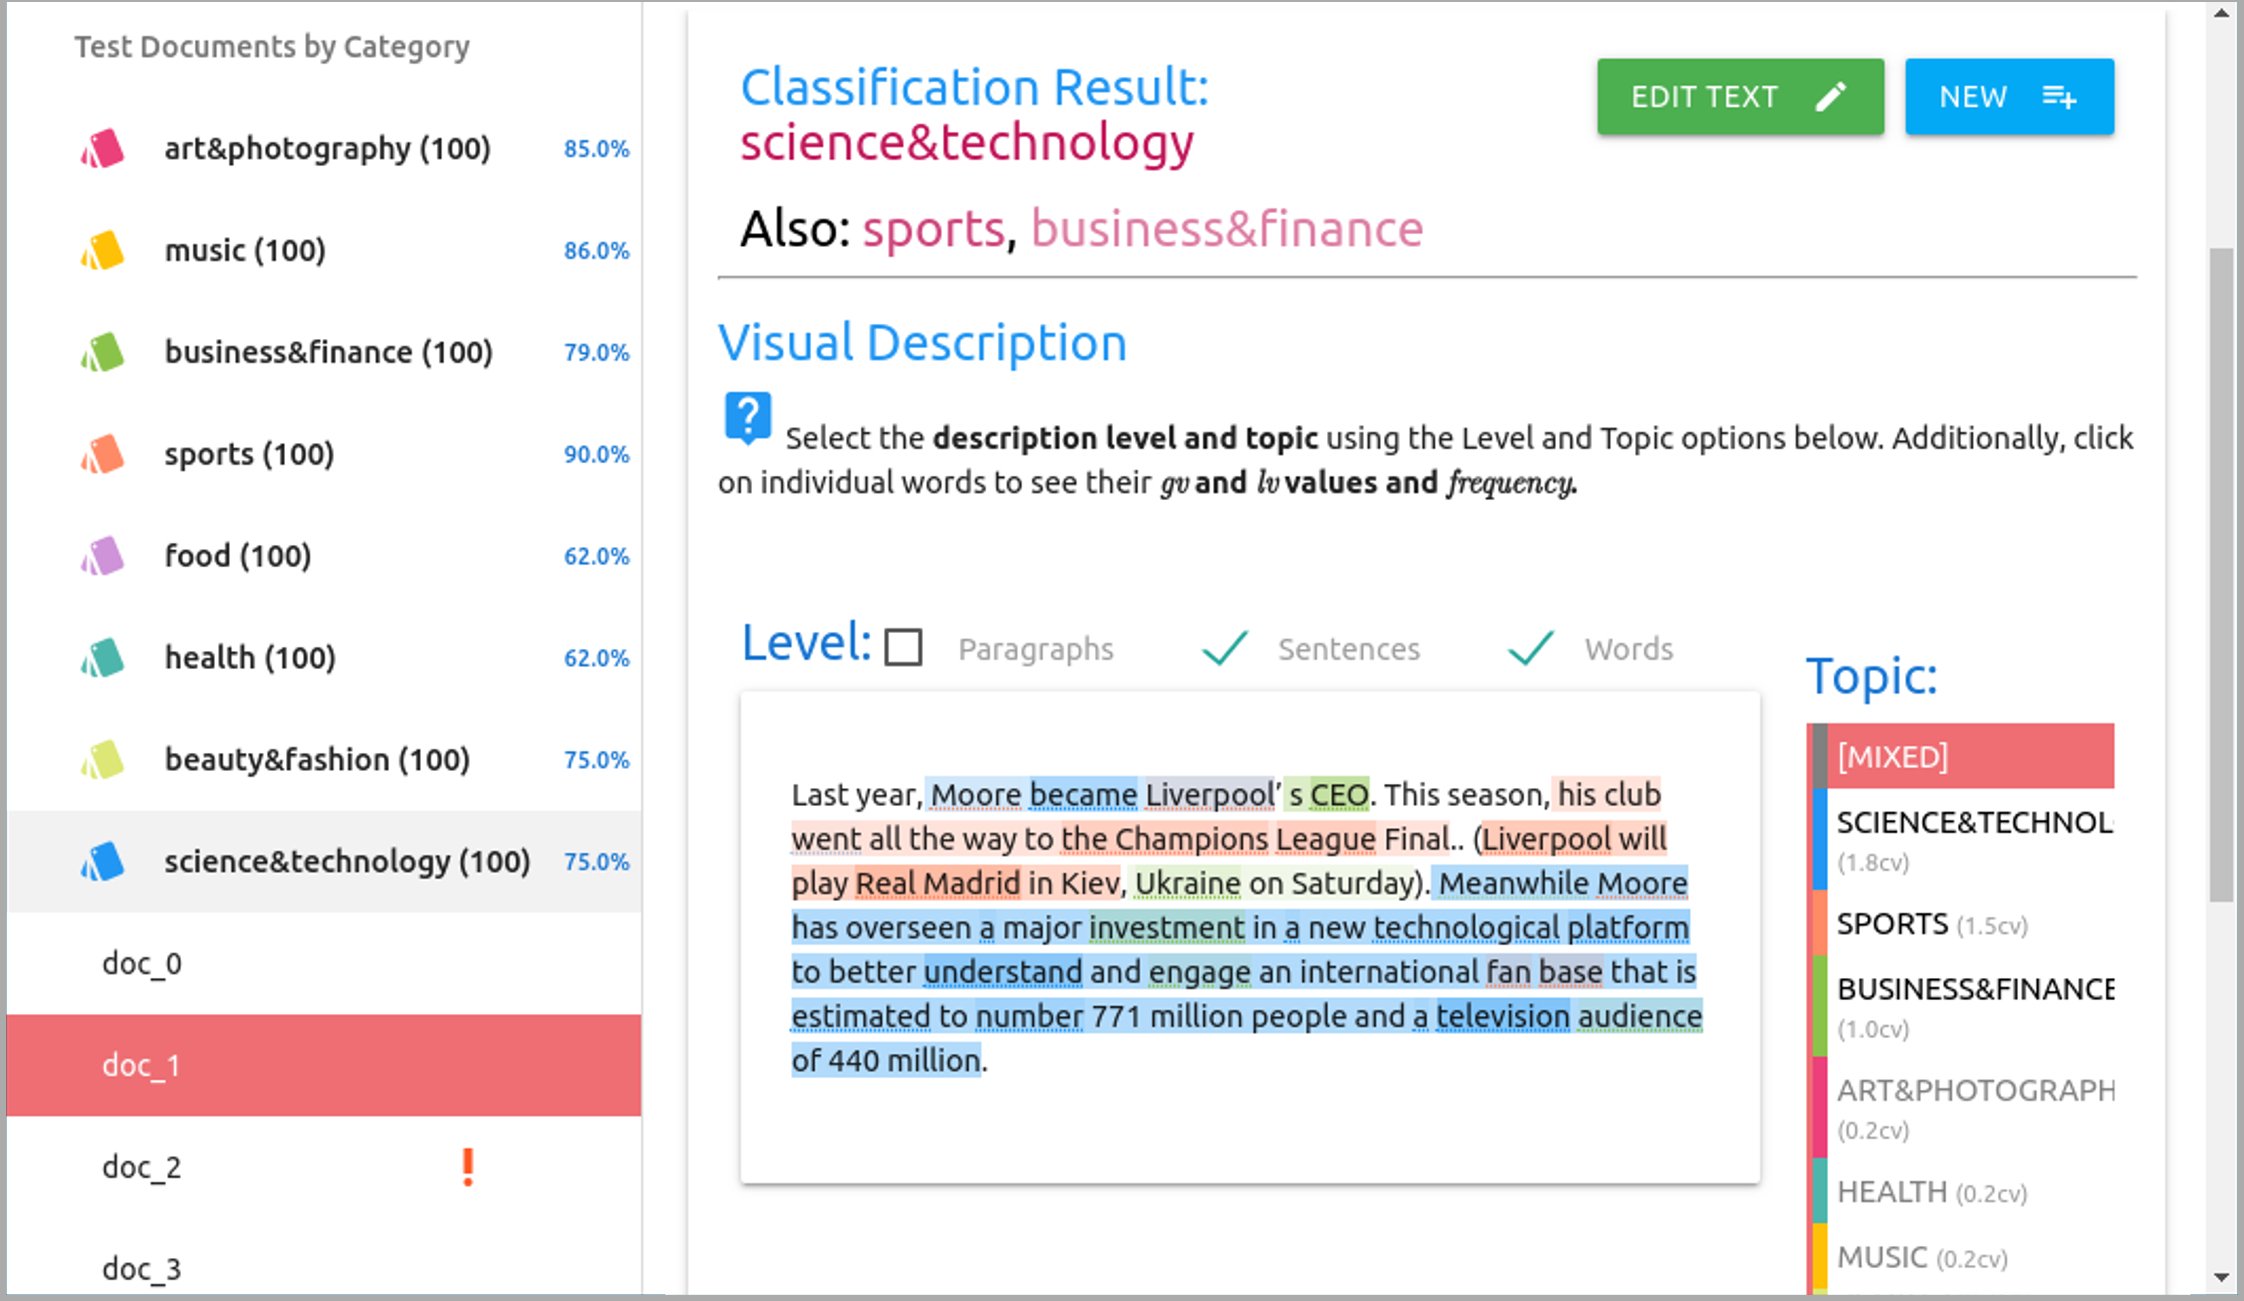
\includegraphics[width=\textwidth]{images/burdisso-fig1}
    \caption{
    Captura de pantalla de la herramienta ``Live Test''. En el panel izquierdo, se muestra la lista de documentos de prueba agrupados por clase, junto con el porcentaje de aciertos para cada una.
    Notar que el documento ``doc\_2'' está marcado con un signo de exclamación (!); esta marca indica que se lo clasificó de forma incorrecta, lo que facilita el análisis de errores.
    En este ejemplo, el usuario ha seleccionado el ``doc\_1'', el resultado de la clasificación se muestra en la parte superior.
    Además, el usuario ha seleccionado que la explicación visual sea dada a nivel de oración y de palabra en simultáneo.
    Por medio de esta explicación el usuario tal vez podría confirmar que el documento fue clasificado correctamente porque, efectivamente, el modelo ha aprendido a reconocer palabras importantes, como ser ``television'' para tecnología, ``Real Madrid'' para deportes o ``investment'' para negocios.
    Además, utilizando los distintos colores, el usuario podría notar que la primera oración pertenecía a varios temas, la segunda cambiaba el tema a deportes (naranja) y, finalmente, de ``Meanwhile'' en adelante, el tema se cambia principalmente a tecnología (azul), y un poco de negocios (verde) dado por las palabras ``investment'', ``engage'' y ``audience''.
    Finalmente, el usuario también podría editar el documento o crear uno nuevo utilizando los dos botones mostrados en la esquina superior derecha.}
    % Live Test screenshot. On the left side, the list of test documents grouped by category is shown along with the percentage of success.
    % Note the ``doc\_2'' document is marked with an exclamation mark (!); this mark indicates it was misclassified, which eases error analysis.
    % The user has selected the ``doc\_1,'' the ``classification result'' is shown above the visual description. 
    % In this figure, the user has chosen to display the visual explanation at sentence-and-word level, using mixed topics.
    % For instance, the user can confirm that, apparently, the model has learned to recognize important words and that it has correctly classified the document.
    % Also, by using the colors, the user could notice that the first sentence belonging to multiple topics, the second sentence shifted the topic to $sports$, and finally, from ``Meanwhile'' on, the topic is shifted to $technology$ (and a little bit of $business$ given by the words ``investment'' or ``engage'' colored in green).
    % Note that the user can also edit the document or even create new ones using the two buttons on the upper-right corner.}
    \label{fig:live_test}
\end{figure*}

La herramienta ``Live Test'' es una herramienta de visualización interactiva que le permite a los usuarios probar sus modelos de forma dinámica, en tiempo real.
% The ``Live Test'' tool is an interactive visualization tool that allows users to test his/her models ``on the fly.''
Esta herramienta se puede iniciar con una sola línea de código utilizando la clase ``Live\_Test'', como se mostrará con un ejemplo en la \autoref{sec:eg-2}.
Una vez iniciada, la herramienta proporciona una interfaz de usuario, como la mostrada en la \autoref{fig:live_test}, mediante la cual los usuarios pueden probar su modelo de forma activa utilizando ya sea los documentos del conjunto de prueba o simplemente escribiendo los suyos.
El objetivo principal de esta herramienta es permitirle a los usuarios analizar y comprender lo que efectivamente están aprendiendo sus modelos, por medio de explicaciones visuales similares a las mostradas al final del \autoref{cap:ss3} y \autoref{cap:tss3}, a diferentes niveles, n-gramas de palabras, oraciones y/o párrafos.
Esta herramienta es la que se utilizó para desarrollar las demos disponibles en línea mencionadas en los capítulos anteriores.\footnote{Disponibles en  \url{http://tworld.io/ss3}}
% This tool can be launched with a single line of python code using the $Server$ class (see \autoref{sec:eg-2} for an example).
% The tool provides a user interface (a screenshot is shown in \autoref{fig:live_test}) by which users can manually and actively test their model using either the documents in the test set or just typing  their own. 
% The tool also allows researchers to analyze and understand what their models are learning by providing an interactive and visual explanation of the classification process at three different levels (word n-grams, sentences, and paragraphs). 
% We recommend trying out the ``Topic Categorization'' or the ``Sentiment Analysis on Movie Reviews'' online live demo available at \href{http://tworld.io/ss3}{\url{http://tworld.io/ss3}}.

Por otro lado, la herramienta ``PySS3 Command-Line'' es una herramienta de línea de comandos interactiva, la cual se inicia desde la línea de comandos del sistema operativo utilizando el comando ``pyss3'', el cual se agrega automáticamente al sistema junto con la instalación del paquete.
Esta herramienta le permite a los usuarios implementar modelos SS3 e interactuar con ellos sin tener que programarlos utilizando Python, sino a través de la utilización de comandos especiales para cada etapa del proceso de desarrollo del modelo. Probablemente una de las características más importantes de esta herramienta es la capacidad de registrar, automática y permanentemente, el historial de cada evaluación que el usuario ha realizado sobre el modelo ---por ejemplo, utilizando validaciones cruzadas o búsquedas en grilla. Luego, los usuarios pueden utilizar este historial de evaluación para visualizar el rendimiento de sus modelos en términos de los distintos valores de los hiperparámetros, por medio del comando ``plot evaluations'' ---como se ilustrará en la \autoref{sec:eg-3}, estas mismas características también están disponibles a través de la clase $pyss3.util.Evaluation$.
% The ``PySS3 Command-Line'' is an interactive command-line tool that  can be started from the operating-system command prompt using the ``pyss3'' command (automatically added to the system when installing the package).
% This tool allows users to deploy SS3 models and interact with them through special commands for every stage of the machine learning pipeline (such as model selection, training, or testing). Probably one of its most important features is the ability to automatically (and permanently) record the history of every evaluation that the user has performed (such as tests, k-fold cross-validations, or grid searches). Users can then use this evaluation history to visualize their models' performance in terms of the hyperparameters' values though the ``plot evaluations'' command. As will be illustrated in \autoref{sec:eg-3}, the same features are also available through the $pyss3.util.Evaluation$ class.

\section{Ejemplos Ilustrativos}
\label{sec:examples}

En esta última sección, se presentan tres simples ejemplos ilustrativos que sirven para mostrar cómo se utiliza efectivamente el paquete en la práctica.
Como se menciona en la documentación del paquete, PySS3 proporciona dos tipos distintos de flujos de trabajo principales.
En el flujo de trabajo clásico, el usuario, como de costumbre, importa las clases y funciones necesarias del paquete, y luego escribe un programa Python para entrenar y probar los clasificadores. En el segundo flujo de trabajo, todo el proceso se realiza por medio de la herramienta ``PySS3 Command-Line'', sin tener que utilizar Python.
En esta sección no mostraremos ejemplos de este último, 
% In this section, we will introduce three simple illustrative examples.
% PySS3 provides two main types of workflow.
% In the classic workflow, the user, as usual, imports the needed classes and functions from the package and then writes a python script to train and test the classifiers. In the ``command-line'' workflow, the whole machine learning pipeline is done using only the ``PySS3 Command-Line'' tool, without coding in Python.
% Due to space limitations, we will not show examples for the latter here.
sin embargo, para ver ejemplos completos para ambos flujos de trabajo, se recomienda realizar alguno de los tutoriales disponibles en la documentación.\footnote{\url{https://pyss3.rtfd.io/en/latest/user_guide/getting-started.html\#tutorials}}
% However, for full working examples using both workflows, please refer to the tutorials in the documentation (\href{https://pyss3.rtfd.io/en/latest/user_guide/getting-started.html#tutorials}{\url{https://pyss3.rtfd.io/en/latest/user_guide/getting-started.html\#tutorials}})
Además, para los lectores interesados en probar el paquete en línea, sin tener que instalar nada en sus sistemas, los tutoriales también se encuentran disponibles en formato de Jupyter Notebooks, las cuales se pueden ejecutar en línea por medio del servicio \emph{MyBinder}.\footnote{Por medio del siguiente enlace: \url{https://mybinder.org/v2/gh/sergioburdisso/pyss3/master?filepath=examples}}
% Additionally, readers interested in trying PySS3 out ``right away'', we have created Jupyter Notebooks for the tutorials, which can be executed online using \emph{MyBinder} (\href{https://mybinder.org/v2/gh/sergioburdisso/pyss3/master?filepath=examples}{\url{https://mybinder.org/v2/gh/sergioburdisso/pyss3/master?filepath=examples}}).

\

Los siguientes ejemplos asumen que el usuario ya ha cargado los documentos de entrenamiento y prueba, y sus correspondientes etiquetas de clase, respectivamente, en las listas $x\_train$, $y\_train$, $x\_test$, $y\_test$, como es usual. Esto se podría llegar a hacer, por ejemplo, con $pyss3$ por medio de la clase ``Dataset'' del submódulo $pyss3.util$, de la siguiente manera:
% In the following examples, we will assume the user has already loaded the training and test documents and category labels, as usual, in the $x\_train$, $y\_train$, $x\_test$, $y\_test$ lists, respectively. For instance, this could be done using the $Dataset$ class from the $pyss3.util$ submodule, as follows:

\begin{minted}[
% frame=lines,
framesep=2mm,
baselinestretch=1.2,
bgcolor=lightgray,
fontsize=\footnotesize,
% linenos
]{python}
from pyss3.util import Dataset

x_train, y_train = Dataset.load_from_files("path/to/train")
x_test, y_test = Dataset.load_from_files("path/to/test")
\end{minted}


\subsection{Entrenamiento y Prueba}
\label{sec:eg-1}

En este pequeño ejemplo se muestra cómo, con unas pocas líneas y de forma similar a con los modelos de \emph{scikit-learn}, se puede entrenar y probar un modelo SS3 utilizando los valores predeterminados.
% This simple example shows how to train and test an SS3 model using default values.

\begin{minted}[
% frame=lines,
framesep=2mm,
baselinestretch=1.2,
bgcolor=lightgray,
fontsize=\small,
% fontsize=\footnotesize,
% linenos
]{python}
from pyss3 import SS3

clf = SS3()
clf.fit(x_train, y_train)

y_pred = clf.predict(x_test)
print("Accuracy:", accuracy(y_pred, y_test))
\end{minted}

La última línea imprime el \emph{accuracy} obtenido ---se asume aquí que la función \emph{accuracy} ya existe, por ejemplo, habiendo sido previamente importada desde \emph{sklearn.metrics}.
Notar que, dado que SS3 ignora el concepto de ``documento'' por su naturaleza, a diferencia de con los modelos de \emph{scikit-learn}, aquí no es necesario crear la matriz documento-término ---en su lugar, simplemente se utiliza directamente el texto (preprocesado) de los documentos de $x\_train$ y $x\_test$, tanto para el entrenamiento como para la prueba, respectivamente.
% The last line prints the obtained accuracy, we are assuming here that this $accuracy$ function already exists (for instance, it was previously imported from $sklearn.metrics$).
% Note that since SS3 creates a language model for each category, we do not need to create a document-term matrix, we are simply using the raw $x\_train$ and $x\_test$ documents for training and test, respectively.


\subsection{Entrenamiento y Prueba Interactiva}
\label{sec:eg-2}

En este ejemplo, al igual que en el anterior, se entrena y prueba el modelo. Sin embargo, en lugar de simplemente usar $predict$ y $accuracy$ para medir el rendimiento del modelo, aquí se utiliza la herramienta ``Live Test'', mostrada anteriormente en la \autoref{fig:live_test}, para analizar y probar nuestro modelo de una forma visual e interactiva, del siguiente modo:
% This example is similar to the previous one. However, instead of simply using $predict$ and $accuracy$ to measure our model's performance, here we are using the ``Live Test'' tool to analyze and test our model visually.

\begin{minted}[
% frame=lines,
framesep=2mm,
baselinestretch=1.2,
bgcolor=lightgray,
fontsize=\small,
% linenos
]{python}
from pyss3 import SS3
from pyss3.server import Live_Test

clf = SS3()
clf.fit(x_train, y_train)

Live_Test.run(clf, x_test, y_test)
\end{minted}

Esta última sentencia será la encargada de ejecutar la herramienta ``Live Test'' localmente en el navegador web, utilizando el clasificador, los documentos, y las etiquetas del conjunto de prueba dados en los argumentos.


Alternativamente, también se podría utilizar la función $clf.extract\_insight()$ que, cuando se aplica a un documento, devuelve la lista de fragmentos de texto involucrados en la decisión de la clasificación, ordenados por valor de confianza. Por ejemplo, supongamos que queremos obtener el fragmento de texto, con el mayor valor de confianza, que SS3 utilizó para clasificar al documento mostrado en la \autoref{fig:live_test} como ``sports'', entonces se podría simplemente utilizar $clf.extract\_insight()$ del siguiente modo:
% Alternatively, we could also use the $clf.extract\_insight()$ function. When this function is applied to a document, it returns the list of text fragments involved in the classification decision, ordered by confidence value. For instance, suppose we need to obtain the text fragment with the highest confidence value that was used to classify the document shown in \autoref{fig:live_test} as ``sports,'' we could use $extract\_insight()$ as follows:

\begin{minted}[
% frame=lines,
framesep=2mm,
baselinestretch=1.2,
bgcolor=lightgray,
fontsize=\small,
% linenos
]{python}
# doc = el mismo documento que se muestra en la Figura 7.1
doc = "Last year, Moore became Liverpool's CEO. This season, ..."

fragments = clf.extract_insight(doc, "sports")

print(fragments[0])
\end{minted}

% Which will print the following (fragment, confidence value) pair:
Lo que imprimirá el siguiente par (fragmento, valor de confianza):

\begin{minted}[
% frame=lines,
framesep=2mm,
baselinestretch=1.2,
bgcolor=lightgray,
fontsize=\small,
breaklines
% linenos
]{python}
('to the Champions League Final. (Liverpool will play Real Madrid in Kiev, Ukraine on Saturday). Meanwhile Moore has',  0.97)
\end{minted}

Este par nos indica que el documento fue clasificado como ``sports'', principalmente, debido a que nuestro modelo encontró este fragmento como perteneciente a ``sports'' con un valor de confianza de $0.97$.\footnote{Se recomienda el tutorial ``\emph{getting the text fragments involved in the classification decision}'' para los lectores interesados en conocer más sobre esta funcionalidad, disponible en  \url{https://pyss3.rtfd.io/en/latest/tutorials/extract-insight.html}} 
% This pair indicates the document was classified as ``sports,'' mainly due to our model finding this fragment as belonging to ``sports'' with a confidence value of $0.97$. Finally, interested readers may refer to the ``getting the text fragments involved in the classification decision'' tutorial available online (\href{https://pyss3.rtfd.io/en/latest/tutorials/extract-insight.html}{\url{https://pyss3.rtfd.io/en/latest/tutorials/extract-insight.html}}).

\subsection{Optimización de Hiperparámetros}
\label{sec:eg-3}

\begin{figure*}[t!]
    \centering
    % \includegraphics[width=190mm]{images/evaluation_plot}
    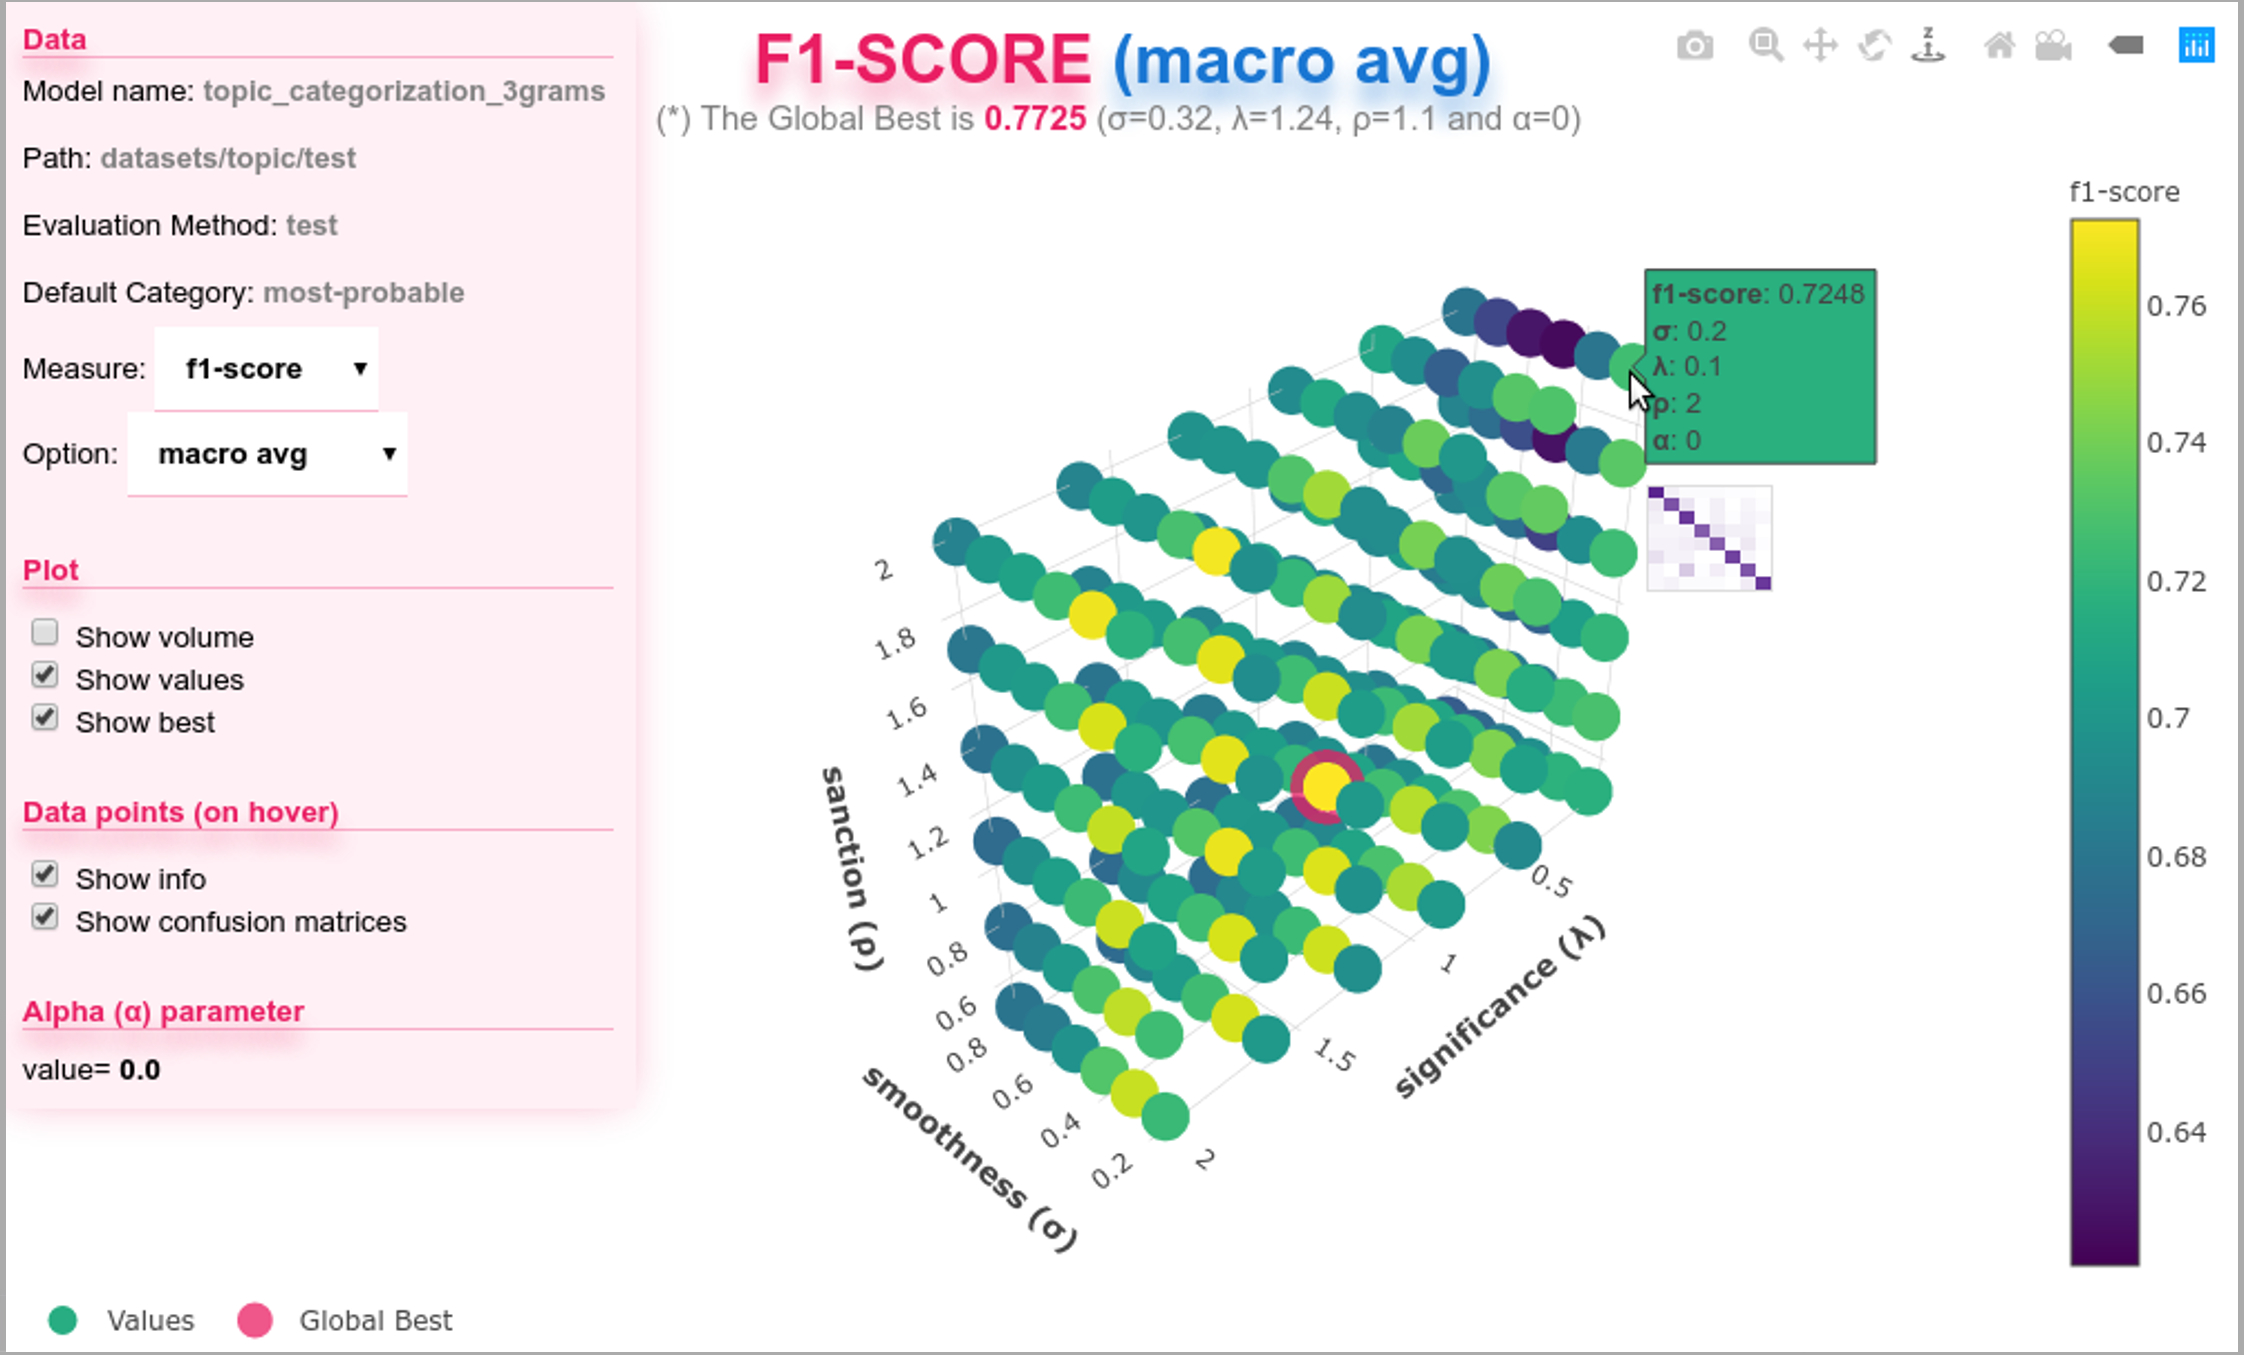
\includegraphics[width=\textwidth]{images/burdisso-fig2}
    \caption{Captura de pantalla del gráfico de evaluación 3D. Cada punto representa una evaluación o experimento realizado utilizando una combinación particular de valores de hiperparámetros. A su vez, estos puntos están coloreados proporcionalmente en relación al desempeño obtenido en esa evaluación. Además, en rosa se colorea el o los puntos que obtuvieron el mejor desempeño global. 
    El usuario puede seleccionar interactivamente la medida de evaluación que desee para medir el desempeño, cambiándola desde el panel de opciones mostrado a la izquierda.
    Además, como se muestra en esta figura, cuando el usuario mueve el cursor sobre un punto en particular, se muestra información relacionada con esa evaluación, incluida una versión simplificada de la matriz de confusión obtenida.}
    % \caption{Evaluation plot screenshot. Each data point represents an evaluation/experiment performed using a particular combination of hyperparameter values. Points are colored proportionally to the obtained performance. The performance measure can be interactively changed using the options panel in the upper-left corner. Additionally, points with the global best performance are marked in pink. As shown in this figure, when the user moves the cursor over a point, information related to that evaluation is displayed, including a small version of the obtained confusion matrix.}
    \label{fig:eval_plot}
\end{figure*}

Este último ejemplo muestra cómo, utilizando la clase ``Evaluation'', se pueden encontrar mejores valores de hiperparámetros para nuestro modelo. En particular, realizaremos la optimización de hiperparámetros por medio de una búsqueda en grilla, utilizando el método $grid\_search$ de la siguiente manera:
% This example shows how we could use the ``Evaluation'' class to find better hyperparameter values for the model trained in the previous example. Namely, we will perform hyperparameter optimization using the \emph{grid search} method, as follows:

\begin{minted}[
% frame=lines,
framesep=2mm,
baselinestretch=1.2,
bgcolor=lightgray,
fontsize=\small,
% linenos
]{python}
from pyss3.util import Evaluation

best_s, best_l, best_p, _ = Evaluation.grid_search(
    clf,
    x_test, y_test,
    s=[0.2, 0.32, 0.44, 0.56, 0.68, 0.8],
    l=[0.1, 0.48, 0.86, 1.24, 1.62, 2],
    p=[0.5, 0.8, 1.1, 1.4, 1.7, 2]
)
\end{minted}

Notar que en PySS3, los hiperparámetros $\sigma$, $\lambda$ y $\rho$  son referidos con las letras ``s'', ``l'' y ``p'', respectivamente.
% Note that in PySS3, the $\sigma$, $\lambda$, and $\rho$ hyperparameters are referenced using the ``s,'' ``l,'' and ``p'' letters, respectively.
Por lo tanto, en esta búsqueda en grilla, $\sigma$ tomará distintos valores diferentes entre $0.2$ y $0.8$, $\lambda$ entre $0.1$ y $2$, y $\rho$ entre $0.5$ y $2$.
% Thus, in this grid search, $\sigma$ will take six different values between $0.2$ and $0.8$, $\lambda$ between $0.1$ and $2$, and $\rho$ between $0.5$ and $2$.
Una vez finalizada la búsqueda, esta función devolverá los mejores valores obtenidos para los tres hiperparámetros, asignándolos respectivamente a $best\_s$, $best\_l$ y $best\_p$.
% Also note that once the grid search is over, the function will return the best hyperparameter values and store them in $b\_s$, $b\_l$, and $b\_p$, respectively.

Luego de realizar la búsqueda en grilla, para poder realizar un mejor análisis del desempeño obtenido en la búsqueda, podríamos utilizar la función $plot()$ para visualizar los resultados con un gráfico tridimensional, de la siguiente manera:
% After performing the grid search, we could also use the $plot()$ function to visualize our results, as follows:

\begin{minted}[
% frame=lines,
framesep=2mm,
baselinestretch=1.2,
bgcolor=lightgray,
fontsize=\small,
% linenos
]{python}
Evaluation.plot()
\end{minted}

Esta función creará en el directorio actual un archivo HTML portátil que contiene un gráfico 3D interactivo, y luego lo abrirá en el navegador web del usuario.
% This function will first save, in the current directory, a single and portable HTML file containing an interactive 3D plot. Then, it will open it up in the web browser.
Por ejemplo, en la \autoref{fig:eval_plot} se muestra una captura de pantalla de este gráfico 3D, en el que podemos ver que los mejores valores de hiperparámetros para esta búsqueda fueron $\sigma=0.32$, $\lambda=1.24$ y $\rho=1.1$.
Finalmente, utilizando la función $clf.set\_hyperparameters()$ podríamos actualizar los hiperparámetros de nuestro modelo con los mejores valores obtenidos, de la siguiente manera:
% For instance, a screenshot of this 3D plot is shown in \autoref{fig:eval_plot}, \footnote{More info available in the documentation (\href{https://pyss3.rtfd.io/en/latest/user_guide/visualizations.html\#evaluation-plot}{\url{https://pyss3.rtfd.io/en/latest/user_guide/visualizations.html\#evaluation-plot}}).} 
% in which we can see that the best hyperparameter values for this search were $\sigma=0.32$, $\lambda=1.24$, and $\rho=1.1$. Finally, using the obtained best values, we could update the hyperparameter values of our already trained model using the $clf.set\_hyperparameters()$ function, as follows:

\begin{minted}[
% frame=lines,
framesep=2mm,
baselinestretch=1.2,
bgcolor=lightgray,
fontsize=\small,
% linenos
]{python}
clf.set_hyperparameters(s=best_s, l=best_l, p=best_p)
\end{minted}

Alternativamente, también podríamos crear y entrenar un nuevo modelo desde cero utilizando manualmente los mejores valores obtenidos:
% Alternatively, we could also create and train a new model using the obtained best values:

\begin{minted}[
% frame=lines,
framesep=2mm,
baselinestretch=1.2,
bgcolor=lightgray,
fontsize=\small,
% linenos
]{python}
clf = SS3(s=0.32, l=1.24, p=1.1)
clf.fit(x_train, y_train)
\end{minted}

\begin{figure}[t!]
    \centering
    % 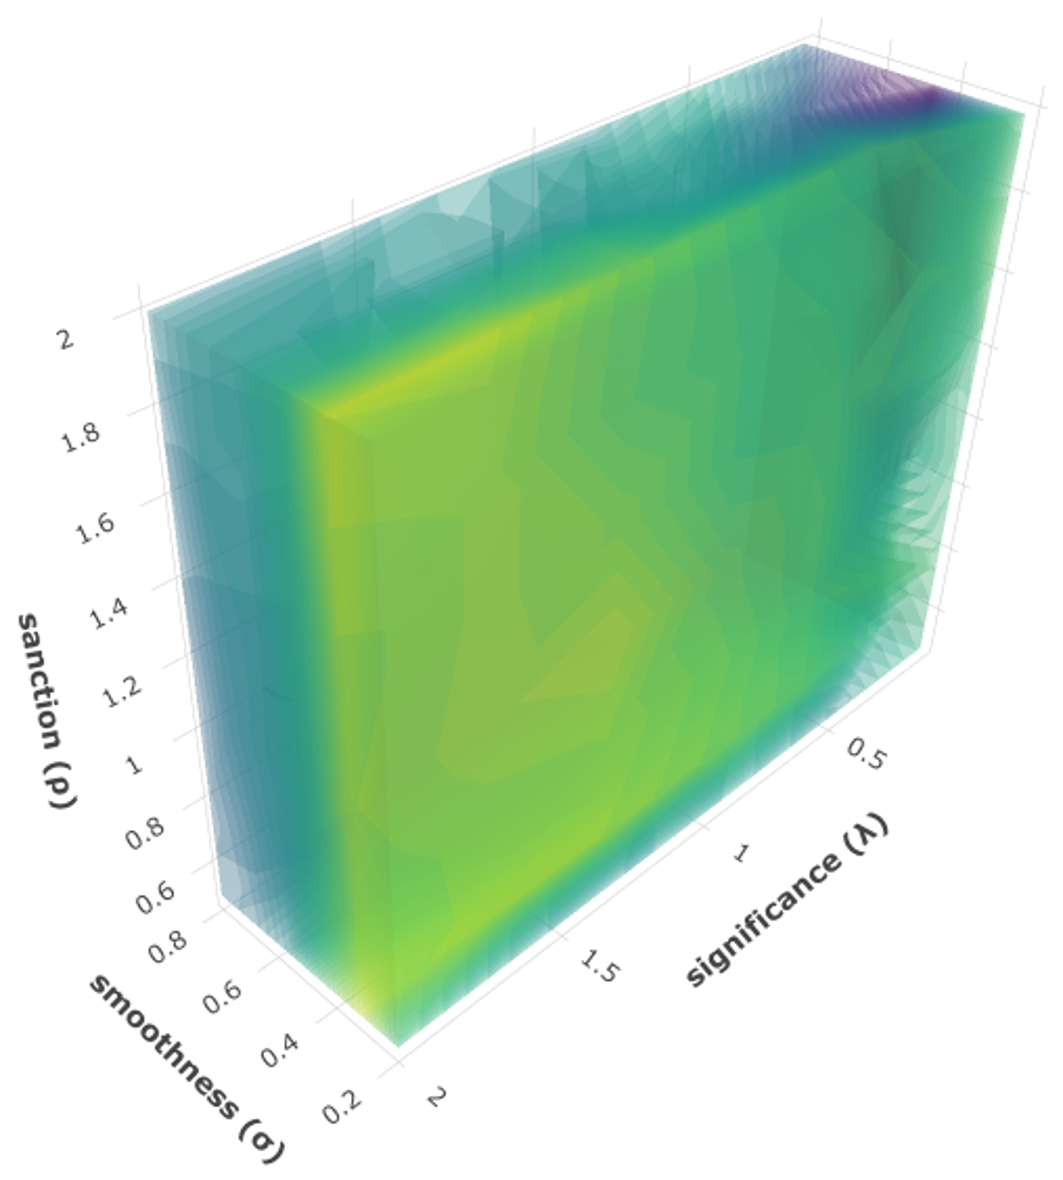
\includegraphics[width=\linewidth]{images/burdisso-fig3}
    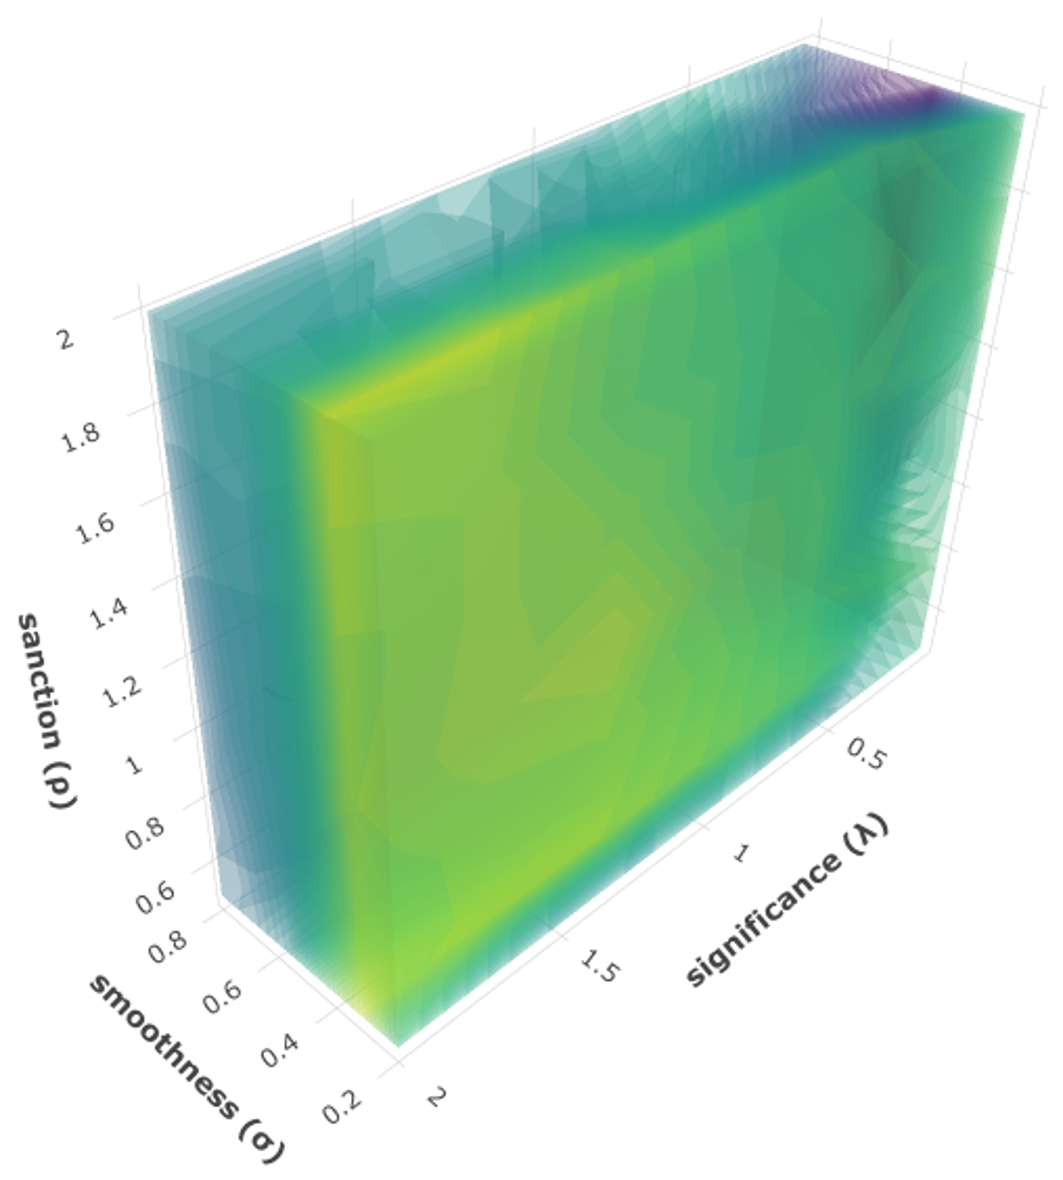
\includegraphics[width=90mm]{images/burdisso-fig3}
    \caption{Gráfico de evaluaciones con la opción ``show volume'' (mostrar volumen) habilitada. Al habilitar esta opción, ahora podemos observar más claramente que el hiperparámetro \emph{sanction} ($\rho$) no parece afectar el rendimiento. Por el contrario, el rendimiento parece aumentar a medida que aumenta el valor de \emph{significance} ($\lambda$) y parece disminuir a medida que el hiperparámetro \emph{smoothness} ($\sigma$) se aleja de $0.35$.}
    % \caption{Evaluation plot with ``show volume'' option enabled.  With this option enabled, we can now more clearly see that the \emph{sanction} ($\rho$) hyperparameter does not seem to impact performance. In contrast, the performance seems to increase as the \emph{significance} ($\lambda$) value increases and seems to drop as the \emph{smoothness} ($\sigma$) hyperparameter moves away from $0.35$.}
    \label{fig:eval_plot_volume}
\end{figure}

Notar que, además de utilizar el gráfico de evaluación 3D para obtener los mejores valores, los usuarios pueden utilizarlo para analizar, y comprender mejor, la relación entre los hiperparámetros y el rendimiento del clasificador dentro del problema particular abordado.
Por ejemplo, si el usuario habilita la opción ``show volume'' desde el panel de opciones, el gráfico se convertirá en una estructura sólida que nos facilitará  realizar este tipo de análisis, como se muestra en la \autoref{fig:eval_plot_volume}. Otra característica positiva de la función $Evaluation.plot()$ es que le permitirá a los investigadores compartir sus gráficos, por ejemplo en sus publicaciones, por medio de los archivos HTML portables generados localmente ---lo que aumentaría la transparencia de las experimentaciones.\footnote{Por ejemplo, hemos subido el archivo HTML generado para el ejemplo mostrado en la \autoref{fig:eval_plot} en línea para que los lectores interesados pueden interactuar con él: \url{https://pyss3.rtfd.io/en/latest/_static/eval_plot.html}}
% Note that, in addition to using the 3D evaluation plot to obtain the best values, users can use it to analyze (and better understand) the relationship between hyperparameters and performance in the particular problem being addressed. 
% For instance, if the ``show volume'' option is enabled from the options panel, the plot will turn into the plot shown in \autoref{fig:eval_plot_volume}. It is worth mentioning that researchers could share these portable files with the 3D plots in their papers, which would increase experimentation transparency. For instance, we have uploaded the file generated for \autoref{fig:eval_plot} online for readers to interact with it (\href{https://pyss3.rtfd.io/en/latest/_static/eval_plot.html}{\url{https://pyss3.rtfd.io/en/latest/_static/eval_plot.html}}).
%\footnote{It is worth mentioning that researchers could share these 3D model evaluation's portable files in their papers, which would increase experimentation transparency. For instance, we have uploaded the file used for the evaluation shown in \autoref{fig:eval_plot} for readers to interact with it: \href{https://pyss3.rtfd.io/en/latest/_static/eval_plot.html}{\url{https://pyss3.rtfd.io/en/latest/_static/eval_plot.html}}}

\section{Observaciones Finales}

En este capítulo hemos introducido brevemente a PySS3, un paquete de Python de código abierto que permite utilizar fácilmente el modelo de clasificación de texto desarrollado como producto de este trabajo de investigación. Además, este paquete incluye una serie de herramientas de visualización útiles que ayudan a comprender mejor lo que el modelo está realmente aprendiendo.
Este software podría ser especialmente útil para investigadores, profesionales o usuarios en general, interesados en implementar modelos más transparentes, y por lo tanto más confiables, para tareas de clasificación de texto.
Finalmente, esperamos continuar el avance y la mejora de PySS3 a través de la ayuda directa o indirecta de todos aquellos que estén interesados y quieran formar parte de este proyecto de código abierto.
% We have briefly introduced PySS3, an open-source Python package that implements a novel machine learning model for text classification that comes with useful visualization tools.
% This software could be especially useful for researchers and practitioners interested in deploying explainable and more reliable models for text classification.
% Finally, we hope to continue the advancement and improvement of PySS3 through the direct or indirect help of those in the mathematical and computer science disciplines who want to be part of this open-source project.
\hfill$\square$

%\part{CONCLUSIONES GENERALES}
%\label{part4}

%\acresetall
%\chapter{Conclusiones y Trabajo Futuro}
%\label{cap:conclusion}
%% Transtornos
    % sacar lo que pusimos en el cap 4 sobre clinica
    % modelo entrenaod con dep y ano para self-harm, se necesitarían trabajo interdicippliario o a futuro para explorar más la relación entre estas problematicas porque los resultados experimentales sugieren que es la relación es lo suficientemetne fuerte como para poder detectar selfharm.

% resumen
En este trabajo hemos introducido, desarrollado, evaluado y analizado a SS3, un clasificador de texto diseñado con el objetivo de abordar escenarios de detección anticipada de riesgos en entornos dinámicos, como el de las redes sociales, de forma eficiente y unificada.
En particular, vimos que este tipo de escenarios es especialmente desafiante para los modelos convencionales debido a que abordarlas involucra, al menos, tres aspectos clave: \emph{clasificación de secuencias}, \emph{clasificación anticipada} y \emph{transparencia/explicabilidad}.
Por consiguiente, SS3 fue diseñado para integrar, respectivamente, las siguientes tres capacidades: \emph{trabajo/funcionamiento incremental}, \emph{soporte de mecanismos de toma de decisión anticipada}, y \emph{capacidad de explicar visualmente las razones detrás de sus decisiones}.

% evaluación y resultados
La evaluación del modelo se llevó a cabo, primeramente, en la tarea de detección anticipada de depresión de la primer edición del eRisk (2017).
Luego, se lo evaluó junto a $\tau$-SS3, una extensión del modelo original, en las dos tareas del eRisk 2018, detección anticipada de anorexia y detección anticipada de depresión. Finalmente, ambos modelos fueron puestos a prueba participando en las dos tareas del eRisk 2019, detección anticipada de anorexia y detección anticipada de conductas autodestructivas.
Los resultados obtenidos fueron, en relación a los otros modelos, consistentemente buenos a lo largo de todas las tareas.
En particular, el modelo obtuvo los mejores valores $ERDE_5$ y $ERDE_{50}$ en las distintas tareas abordadas y, en relación a las nuevas medidas introducidas en el eRisk 2019, obtuvo el mejor valor para la medida $F_{latency}$ en la detección anticipada de conductas autodestructivas, y el mejor desempeño general para las medidas basadas en ranking en ambas tareas de esa edición del eRisk ---habiendo conseguido los mejores valores $P@10$ y  $NDCG@10$, consistentemente, en los cuatros rankings y en las dos tareas utilizadas para evaluarlo, junto a los mejores valores $NDCG@100$ para los rankings generados con 1 y 100 publicaciones, y los segundos mejores para los generados con 500 y 1000, en ambas tareas.
Además, como SS3 fue diseñado para poder trabajar incrementalmente, permitiéndole procesar secuencias en tiempo $O(n)$ con respecto a la longitud de las mismas, los resultados también mostraron que el modelo es computacionalmente eficiente al haber sido el más rápido en las distintas tareas.
Finalmente, los resultados sugieren que SS3 puede llegar a ser un modelo robusto, ya que, independientemente de los datos utilizados para entrenarlo, su desempeño se mantuvo consistente a lo largo de las distintas tareas y medidas de desempeño utilizadas para evaluarlo, a pesar de haber utilizado el mismo valor de hiperparámetros para todas ellas.
Además, otro aspecto interesante a destacar es su simpleza e independencia del dominio, ya que no utilizó ningún tipo de representaciones de documentos compleja, o manualmente creada, ni mecanismos complejos de clasificación anticipada específicos para cada dominio abordado ---lo que contrasta con otros modelos que requerirían de un proceso costoso para adaptarlos a nuevos problemas.

% trabajo a futuro
% Sin embargo, si bien SS3 tuvo un desempeño superior en relación a los otros modelos, su desempeño se encontró lejos de ser perfecto.
% Por ejemplo, si bien los valores $ERDE$ fueron los menores de entre los demás modelos, no fueron lo suficientemente cercanos a $0$ como para indicar un desempeño sobresaliente en términos absolutos ---valores cercanos a $0$ indicarían una clasificación rápida y precisa, con un porcentaje de error cercano a nulo.
% Lo mismo se pudo apreciar en relación a la medida $F_{latency}$, en donde el valor obtenido para la tarea de detección anticipada de anorexia del eRisk 2019 no fue el mejor, o en la tarea de detección de conductas autodestructivas, en donde si bien obtuvo el mejor valor ($0.52$), dicho valor se encontró lejos de ser sobresaliente, es decir, cercano a $1$.
% Este hecho nos señala que, si bien los resultados obtenidos fueron alentadores, aún se requiere de mucho trabajo para que, de hecho, se puedan desarrollar sistemas realmente eficientes en detectar automática y anticipadamente situaciones de riesgo, en la práctica.
Sin embargo, si bien los resultados obtenidos fueron alentadores en relación a los otros modelos, todavía se tiene mucho margen de mejora en términos absolutos como para que, de hecho, se puedan desarrollar sistemas realmente eficientes en detectar automática y anticipadamente situaciones de riesgo, en la práctica.
Por este motivo, como trabajo futuro, planeamos explorar diferentes aspectos vinculados a mejorar el desempeño de clasificación anticipada del modelo.
En este contexto, creemos que los resultados obtenidos en las medidas basadas en ranking son claves, ya que nos señalan que SS3, de hecho, aprendió a valorar correctamente el nivel de riesgo de los usuarios y que, por lo tanto, si no obtuvo un mejor desempeño en la clasificación no se debió a una mala estimación de dicho valor, sino a la política utilizada para decidir \emph{cuándo} clasificarlos anticipadamente en base al mismo.
En particular, la política utilizada mostró ser ``demasiado precoz'' al  priorizar, con diferencia, velocidad por sobre exactitud ---habiendo clasificado a los posibles usuarios en riesgo luego de procesar sólo 3 de sus publicaciones, en promedio.
En consecuencia, como trabajo futuro exploraremos mejores políticas de clasificación anticipada, por ejemplo, creemos que retrasar la clasificación hasta que el nivel de riesgo estimado del usuario sea lo suficientemente alto o utilizar una política que haga uso de información global, relacionada al nivel de riesgo de todos los usuarios, podría ayudar a mejorar significativamente el rendimiento del clasificador.
Además, buscaremos distintos valores de hiperparámetros que nos permitan mejorar el rendimiento en términos de la nueva medida $F_{latency}$, ya que los utilizados fueron seleccionados en relación a la medida $ERDE$. %---la cual prioriza, en gran medida, velocidad y \emph{recall} por sobre precisión.
Asimismo, también realizaremos pruebas utilizando diferentes \emph{operadores de resumen}, $\oplus_j$, ya que en este trabajo no se lo consideró y podría tener un impacto positivo en el desempeño del modelo. Estos \emph{operadores de resumen} podrían hasta incluso llegar a ser funciones complejas que sean capaces de realizar operaciones más avanzadas que una simple operación aritmética dada, ya que en principio se podría utilizar cualquier algoritmo que tome como entrada una lista de vectores y retorne un único vector, por ejemplo, estos \emph{operadores de resumen} se podrían hasta incluso aprender utilizando modelos de aprendizaje automático.
Finalmente, al igual que con $\tau$-SS3, también exploraremos otras maneras de extender el modelo, por ejemplo, se podrían explorar formas alternativas para calcular el \emph{valor global}, $gv(w,c)$, ya sea utilizando nuevas ecuaciones o realizando mejoras sobre las actuales.
Además, en relación a una nueva extensión, creemos que utilizar información sobre la coocurrencia de las palabras podría contribuir positivamente en el desempeño del modelo para tareas como las abordadas, ya que las palabras que coocurran con palabras tales como ``I'', ``myself'' o ``my'' podrían ser muy discriminativas, permitiéndole al modelo detectar oraciones completas en las que el autor se refiere a sí mismo ---esta extensión se podría implementar, por ejemplo, utilizando un grafo de coocurrencia por cada clase, en donde cada arista de los grafos esté ponderada por su \emph{valor global}, aprendido en base al \emph{valor local} de dicha artista a lo largo de los distintos grafos.

Por otro lado, ya que el modelo introducido es en esencia un clasificador de texto de propósito general, este trabajo doctoral habilita nuevas líneas de investigación no vinculadas específicamente a la detección anticipada de riesgos, tales como las vinculadas a examinar distintas propiedades del clasificador, su desempeño en diferentes tipos de tareas, o su integración con otros modelos.
Por ejemplo, en este trabajo pudimos observar, tanto cualitativamente por medio de las nubes de palabras como cuantitativamente en base a los resultados basados en ranking, que el \emph{valor global} puede ser un buen estimador de la importancia de las palabras en relación a cada clase, por lo que creemos que podría jugar un papel importante, por ejemplo, como método de pesado de término o como método de selección de características. Por lo tanto, como trabajo futuro utilizaremos al \emph{valor global} como método de pesado de términos y selección de características, comparándolo con otros enfoques bien conocidos, como la \emph{ganancia de información}, \emph{chi-cuadrado} ($\chi^2$), \emph{tf-idf}, entre otros.
De igual modo, examinaremos la integración de los \emph{vectores de confianza} producidos por SS3 en otros modelos, por ejemplo, al utilizarlos para construir nuevas representaciones vectoriales, densas, de los documentos de entrada, o al utilizarlos como ``embeddings supervisados'' de distintos bloques de texto\footnote{Por ejemplo, embeddings de palabras, embeddings de oraciones, embeddings de documentos, etc.} ---los cuales luego podrían ser integrados, por ejemplo, a modelos secuenciales tales como redes neuronales convolucionales o distintos tipos de redes neuronales recurrentes, como las LSTM o las GRU.
Además, sería interesante probar la robustez del modelo ante ciertos problemas bien conocidos dentro del área.
Por ejemplo, en base a que el modelo ve a cada clase como una ``gran bolsa de palabras'' en donde el número de documentos utilizados para construirlas durante el entrenamiento es irrelevante,\footnote{Siempre que la frecuencia relativa de las palabras sea la adecuada.} y en base a los resultados obtenidos, en donde los conjuntos de datos utilizados fueron altamente desbalanceados, creemos que el modelo podría tener cierta robustez ``natural'' ante el conocido \emph{problema de desbalance de clases}, por lo que realizaremos pruebas en distintas tareas para poder cuantificar dicha robustez.
Del mismo modo, al aprender a ponderar las palabras globalmente, sin vincularse directamente a cada documento, sus propiedades o su origen, el modelo tal vez podría llegar a tener cierta robustez para lidiar con el problema de la \emph{clasificación en dominios cruzados}, como podrían sugerirlo los resultados obtenidos por el modelo \emph{UNSL\#3} en la tarea de detección de conductas autodestructivas del eRisk 2019, el cual mostró un buen desempeño en relación a los otros modelos, a pesar de haber sido entrenado con datos de anorexia y depresión.
Finalmente, sería interesante medir el desempeño del clasificador en distintas tareas de clasificación de documentos tradicionales, no sólo en clasificación de etiquetado único sino también de multi-etiquetado,\footnote{En inglés, ``single-label clasification'' y ``multi-label clasification'', respectivamente.} ya que no hay ninguna restricción que le impida al modelo asignarle más de una clase al documento de entrada, por lo que también examinaremos el uso de distintas políticas para seleccionar múltiples clases a partir del \emph{vector de confianza} del documento.

\

Por último, dada la naturaleza de la problemática abordada, creemos adecuado concluir este trabajo, al igual que en el \autoref{cap:ss3}, volviendo a remarcar algunos aspectos vinculados a las implicaciones y consideraciones clínicas, y éticas, en relación a su aplicación en la vida real.
% Por último, dada la naturaleza de la problemática abordada, creemos adecuado concluir este trabajo, al igual que en el \autoref{cap:ss3}, con algunos aspectos vinculados a las implicaciones y consideraciones clínicas y éticas del trabajo realizado, en relación a su aplicación en la vida real.
% concluir con algunos aspectos vinculados a posibles aplicaciones las implicaciones y consideraciones clínicas del trabajo realizado.
% mencionar nuevamente, como en la \autoref{sec:implications_clinical}, algunos aspectos vinculados a las implicaciones y consideraciones clínicas del trabajo realizado.
% Los métodos de detección automática pueden ayudar a identificar a personas en riesgo a través del monitoreo pasivo, a gran escala, de las redes sociales, y en el futuro pueden complementar los procedimientos de detección existentes~\cite{guntuku2017detecting}.
% En este contexto, el modelo presentado en este trabajo se pensó como una herramienta que podría ser utilizada, en un futuro, para desarrollar sistemas de monitoreo pasivo a gran escala con los que ayudar a detectar usuarios en riesgo analizando sus patrones lingüísticos. Por ejemplo, dicho sistema podría filtrar usuarios presentando posibles candidatos a profesionales de la salud mental para ser analizados manualmente ---tal vez por medio de un ranking de candidatos ordenados por nivel de riesgo, junto con información visual e interactiva.
El modelo presentado en este trabajo se pensó como un marco de trabajo que podría ser utilizada, a futuro, para desarrollar sistemas de monitoreo pasivo a gran escala con los que ayudar a detectar usuarios en riesgo analizando sus patrones lingüísticos. Por ejemplo, dicho sistema podría filtrar usuarios presentando posibles candidatos a profesionales de la salud mental para ser analizados manualmente ---tal vez por medio de un ranking de candidatos ordenados por nivel de riesgo, junto con información visual e interactiva.
El aspecto de ``monitoreo pasivo a gran escala'' podría estar respaldado por la naturaleza paralelizable e incremental de SS3,\footnote{Sólo sería necesario almacenar un pequeño vector bidimensional por cada usuario, su \emph{vector de confianza}, el cual se actualizaría poco a poco a medida que se genere nuevo contenido.} mientras que la presentación de ``información visual e interactiva'' a los profesionales, por su capacidad de explicar visualmente las razones detrás de sus decisiones.
Está claro que el trabajo presentado en esta tesis doctoral \emph{no persiguió un objetivo de diagnóstico automático}, sino el desarrollo, a futuro, de herramientas de monitoreo complementarias a otros métodos bien establecidos dentro del estudio de la salud mental.
No obstante, los problemas éticos y legales sobre la privacidad y protección de datos que involucraría llevar realmente a la práctica sistemas de monitoreo de este tipo siguen siendo problemas abiertos de investigación~\cite{guntuku2017detecting}. \hfill$\square$

% Finalmente, aunque la interpretación clínica de los resultados no se abordó en nuestro trabajo, es importante resaltar algunos puntos importantes.
% En primer lugar, fue interesante observar que la mayoría de las 100 palabras identificadas por SS3, seleccionadas por mayor \emph{valor global}, se corresponden perfectamente a las categorías habitualmente identificadas en otros estudios más clínicos sobre depresión ---tales como palabras relacionadas a síntomas, tratamientos, divulgación/revelación (disclosure), relaciones/vida (relationships-life) \cite{ de2013social}.



\startbibliography
\newpage\null\thispagestyle{empty}\newpage
\begin{singlespace} % Bibliography must be single spaced
    \bibliography{references}   % Use the BibTeX file ``References.bib''.
\end{singlespace}

\end{document}